\documentclass[a4paper]{article}

%% Language and font encodings
\usepackage[spanish]{babel}
\usepackage[utf8x]{inputenc}
\usepackage[T1]{fontenc}

%% Sets page size and margins
\usepackage[a4paper,top=3cm,bottom=2cm,left=3cm,right=3cm,marginparwidth=1.75cm]{geometry}

\usepackage{xcolor}
\usepackage{listings}
\lstset{basicstyle=\ttfamily,
  frame=tb, % draw a frame at the top and bottom of the code block
  tabsize=2, % tab space width
  showstringspaces=false,
  commentstyle=\color{red},
  keywordstyle=\color{blue},
  breaklines=true
}

%% Useful packages
\usepackage{amsmath}
\usepackage{graphicx}
\usepackage[colorinlistoftodos]{todonotes}
\usepackage[colorlinks=true, allcolors=blue]{hyperref}
\usepackage{amsmath}%
\usepackage{MnSymbol}%
\usepackage{wasysym}%
\usepackage{wrapfig}
%% para los pseudocodigos:
\usepackage{algpseudocode}
\usepackage{algorithm}
\usepackage{verbatim}
%% para definir los forEach
\algnewcommand\algorithmicforeach{\textbf{for each}}
\algdef{S}[FOR]{ForEach}[1]{\algorithmicforeach\ #1\ \algorithmicdo}

\definecolor{mygray}{gray}{0.9}

%Instrucción para evitar poner todos los parrafos con sangría de 0cm

\setlength{\parindent}{0cm}

\title{Diseño de Algoritmos}
\author{Alumnos del curso de Programación 3 del segundo semestre del año 2018}

\begin{document}

\maketitle	
\newpage  
\tableofcontents
\newpage

\newpage



% prueba desde TexStudio
% prueba desde Overleaf
% pull desde Overleaf, modificado y pull desde TexStudio


\section*{Introducción}

Bajo ningún concepto estas notas pretender ser un sustituto natural del libro "Algorithm Design" de Jon Kleinberg y Éva Tardos, sino una simple adaptación y traducción al curso de Programación 3 de la Facultad de Ingeniería de la UDELAR. \\

Estimado lector, esperemos que le sea de utilidad para futuros cursos y sepa disculpar los errores de traducción y sintaxis que puedan existir. Dichos errores podrán ser corregidos por los docentes del curso de P3 o por futuras generaciones.\\

Sólo resta agradecer por el apoyo en traducción y escritura de los siguientes alumnos: \textbf{Bianca López}, \textbf{Richard Busca}, \textbf{Facundo Gutierrez},\textbf{ Mathias Battistella}, \textbf{Damián Sire}, \textbf{Camila Spinelli}, \textbf{Darwin Araujo},  \textbf{Matías Rodriguez}, \textbf{Diego Helal} y \textbf{Matías Iglesias}. \\

\begin{center}
\huge{¡Qué lo disfrute!}
\end{center}



\newpage

\section{ Algunos Problemás Representativos}
\subsection{Primer Problema: Emparejamiento Estable}
Como tema de apertura, nos centraremos en un problema algorítmico que representa muy bien muchos de los temás que van a ser tratados. Motivado por algunas preocupaciones, a partir de las cuales formulamos una clara y simple solución. El algoritmo para resolver el problema es muy claro,  y gran parte de nuestro trabajo será ocupado en probar que es correcto, y dando un límite aceptable en el tiempo que le toma llegar a una respuesta- El problema en si mismo, tiene diversos orígenes.

\subsubsection*{El problema}
El problema de Emparejamiento Estable tiene sus orígenes, en parte, en 1962, cuando David Gale y Lloyd Shapley, dos matemáticos economistas estadounidenses, se hicieron la siguiente pregunta: “¿Puede uno diseñar un proceso de admisión para un colegio, o un proceso de reclutamiento para un empleo, que fuera autoevaluable?”  ¿Qué quiere decir esto?
\\
\\
	Para establecer la pregunta, pensemos primero informalmente sobre el tipo de situación que puede surgir cuando un grupo de amigos, todos estudiantes de Ciencias de la Computación, comienzan a postularse para trabajos de verano. El quid del proceso de postulación es la interacción entre dos tipos de partes: compañías (empleadores) y estudiantes (postulados). Cada postulante tiene un orden de preferencias sobre las compañías, y cada compañía, una vez que reciben la postulación, forma una lista ordenada de los postulantes preferenciales, basada en sus intereses. Las empresas le hacen ofertas a algunos de sus postulantes, los postulantes eligen que oferta aceptar, y todos comienzan sus trabajos de verano.  
\\
\\
	Gale y Shapley consideraron la clase de cosas que pueden ir mal en este proceso, en la ausencia de algún mecanismo que haga cumplir el status quo. Supongamos que tu amigo Raj, ha aceptado un trabajo de verano en CluNet, una gran empresa de telecomunicaciones. Unos días después, la pequeña start-up WebExodus, que tuvo un retraso en las decisiones finales, decide llamar a Raj y también ofrecerle un puesto de trabajo. Ahora Raj, que prefiere Web Exodus antes que CluNet - vencido quizás por la atmósfera de tranquilidad y de “todo puede pasar” -, podría rechazar la oferta de CluNet y aceptar el puesto en WebExodus.  Rápidamente, ante la pérdida de la oferta, CluNet le hace una oferta a uno de sus postulantes en lista de espera, quien rechaza la oferta anterior de la gigante del Software Babelsoft, y la situación se transforma en un espiral fuera de control.
\\
\\
	Las cosas se ven tan mal, o peor, desde la otra perspectiva. Supongamos que una amiga de Raj, Chelsea, destinada a ir a Babelsoft, pero habiendo escuchado la historia de Raj, llama a la gente de WebExodus y les dice, “Saben, prefiero pasar el verano trabajando con ustedes que en Babelsoft”. Ellos encontraron esto fácil de creer, y, mirando la postulación de Chelsea, se dieron cuenta que era preferible contratarla a ella que a otro de los que estaban ya programados para trabajar ahí. En este caso, si WebExodus fuera una empresa con menos escrúpulos, buscarían la forma de retractar su oferta a otro estudiante, y contratar a Chelsea.
\\
\\
	Situaciones como esta pueden generar mucho caos rápidamente, y mucha gente (tanto empleadores como postulantes), pueden terminar insatisfechos con el proceso tanto como con el resultado. ¿Qué salió mal? Un problema básico es que el proceso no es autoevaluable. Si las personas pueden actuar de acuerdo a sus intereses, corren el riesgo de fracasar.
\\
\\
	Bien podríamos preferir la siguiente situación más estable, en la cual el interés personal impide que las ofertas sean rechazadas y se redirijan. Consideremos otro estudiante, quien arreglo ocupar su verano en CluNet. Sin embargo, llama a WebExodus y les revela que también preferiría trabajar para ellos.	Pero en este caso, basada en las postulaciones aceptadas, ellos son capaces de responder “No, resulta que preferimos a otro estudiante al que hemos aceptado, antes que a tí, así que lo lamentamos, pero no hay nada que podamos hacer”. O consideren un empleador, siguiendo seriamente su lista de mejores postulantes, y siendo respondido por cada uno de ellos “No, estoy feliz donde estoy”. En este caso, todos los resultados son estables, no hay más tratos que puedan realizarse.
\\
\\
	Entonces esta es la pregunta que Gale y Shapley se hicieron: Dado un conjunto de preferencias sobre empleadores y postulantes, ¿podemos asignar postulantes a empleadores de forma que cada empleador E, y cada postulante P, que no esté programado para trabajar para E, al menos de una de las siguientes formás?
    \begin{enumerate}
       \item E prefiere a uno de sus postulantes aceptados antes que a P
       \item  P prefiere su situación actual antes que trabajar para E
    \end{enumerate}
Si esto se cumple, la salida es estable: los intereses personales prevendrán cualquier trato entre empresas y postulantes, detrás de escenas.
	\\
    \\
	Gale y Shapley proceden a desarrollar un llamativo algoritmo que soluciona este problema, el cual discutiremos ahora. Antes de hacerlo, notemos que este no es el único origen del Problema del Emparejamiento Estable. Resulta que por una década antes del trabajo de Gale y Shapley, desconocido para ellos el “Programa Nacional de Concordancia de Residentes”, había estado usando a procedimiento muy similar, con la misma motivación, para emparejar residentes a hospitales. En efecto, este sistema con unos pocos cambios se usa en la actualidad.
\\
  \\
	Este es un testimonio del atractivo fundamental del problema. Y desde el punto de vista de este libro, nos provee con un buen primer dominio en el que basándonos sobre algunas definiciones básicas de combinatoria los algoritmos se construyen sobre ellas. 
\subparagraph{FORMULANDO EL PROBLEMA} Para llegar a la esencia de este concepto, ayuda a que el problema sea lo más claro posible. El mundo de las empresas y los postulantes contiene algunas asimetrías que distraen. Cada postulante busca una única compañía, pero cada compañía, está en busca de más de un postulante; además, pueden haber más (o incluso menos) postulantes que puestos. Finalmente, cada postulante no se postula para todas las compañías.\\

Es útil, al menos al principio, eliminar estás complicaciones y lograr una versión más resumida del problema: cada uno de los $n$ postulantes se postula a cada una de las $n$ compañías, y cada compañía va a aceptar a un único postulante. Veremos que haciendo esto se preservan las cuestiones fundamentales del problema; en particular, nuestra solución a esta versión simplificada se extenderá a un caso más general.\\

Siguiendo a Gale y Shapley, notamos que este caso especial puede ser visto como el problema de idear un sistema por el cual cada uno de $n$ hombres y $n$ mujeres pueden terminar contrayendo matrimonio: nuestro problema naturalmente es análogo a dos “géneros” (los postulantes y las compañías), y en el caso que estamos considerando, cada uno está buscando ser emparejado con exactamente un individuo del género opuesto.\\

Entonces, consideremos un conjunto $M =\{m_1, ...,m_n\}$ de $n$ hombres, y un conjunto  $W =\{w_1, ...,w_n\}$ de $n$ mujeres. Denotaremos $M$ x $W$ al conjunto de todos los posibles pares ordenados de la forma $(m, w)$, donde $m \in M$ y  $w \in W $. Un emparejamiento $S$ es un conjunto ordenado de pares, cada uno perteneciente a $M$ x $W$, con la propiedad que cada miembro de $M$ y cada miembro de W aparece a lo sumo en un par de $S$. Un emparejamiento perfecto $S’$ es un emparejamiento con la propiedad de que cada miembro de $M$ y $W$ aparece en exactamente en un par de $S’$.\\
 
Los emparejamientos, y los emparejamientos perfectos son objetos a los que recurrimos frecuentemente en estas notas; estos surgen naturalmente modelando una amplia gama de problemas algorítmicos. En la situación actual, un perfecto emparejamiento corresponde simplemente a una manera de emparejar los hombres y las mujeres, de modo que todos terminen casados con alguien, y que nadie este casado con dos personas.
\\
Ahora podemos agregar la noción de preferencias en este conjunto. Cada hombre $m \in M$  clasifica en orden de preferencia a todas las mujeres; diremos que $m$ prefiere a $w$ antes que $w’$, si $m$ clasificó a $w$ más alto que a $w’$. Nos referiremos a la clasificación ordenada de $m$ como su lista de preferencias. No permitiremos vínculos en la clasificación. Cada mujer, análogamente, clasifica a los hombres. \\

Si se da un emparejamiento perfecto S, ¿qué podría salir mal? Guiados por nuestra motivación inicial en termino de empleadores y postulantes, nos puede preocupar la siguiente situación:  hay dos pares $(m, w)$ y $(m’, w’)$ en $S$ con la característica de que $m$ prefiere a $w’$ y $w’$ prefiere a m antes que a $m’$. En este caso, no hay anda que impida que $m$ y $w’$ abandonen sus actuales parejas y se junten; el conjunto de matrimonios no es autoevaluable. Diremos que el par $(m,w’)$ es inestable respecto a $S$: $(m,w’)$ no pertenece a $S$, pero cada $m$ y $w’$ prefiere a el otro como su compañero en $S$. 
\\
   
Nuestra meta es un conjunto de matrimonio que no tenga inestabilidades. Diremos que un emparejamiento $S$ es estable si: es perfecto, y no hay inestabilidad con respecto a $S$. Dos preguntas surgen inmediatamente:
\\
\begin{itemize}
      \item ¿Existe algún emparejamiento estable para cada conjunto de listas de preferencia?
  \item Dado un conjunto de listas de preferencias, ¿podemos construir eficientemente un emparejamiento estable si ya hay uno? 
    \end{itemize}

\subsubsection*{Algunos Ejemplos} Para ilustrar estas definiciones, consideraremos las siguientes dos instancias de un Problema de Emparejamiento Estable.\\

	Primero, supongamos que tenemos un conjunto de dos hombres, $(m,m')$, y un conjunto de dos mujeres, $(w, w’)$.  Las listas de preferencias son las siguientes:

   \begin{itemize}
      \item $m$ prefiere a $w$ antes que a $w’$.
      \item $m’$ prefiere a $w$ antes que a $w’$.
      \item $w$ prefiere a $m$ antes que a $m’$.
      \item $w’$ prefiere a $m$ antes que a $m’$.
    \end{itemize}
	Si pensamos sobre este conjunto de listas de preferencias, intuitivamente, representa un acuerdo completo: los hombres coinciden en el orden de mujeres, y las mujeres coinciden en el orden de los hombres. Aquí hay un único emparejamiento estable, consiste en los pares $(m,w)$ y $(m’,w’)$. El otro emparejamiento perfecto, consiste en los pares $(m’,w)$ y $(m,w’)$, que no será un emparejamiento estable, porque el par $(m,w)$ forma una inestabilidad con respecto a su emparejamiento. (Ambos estarían dispuestos a dejar a sus respectivas parejas para formar una nueva.)
    \\
    \\
A continuación, hay un ejemplo donde las cosas son un poco más complejas. Supongamos que las preferencias son: 
   \begin{itemize}
      \item $m$ prefiere a $w$ antes que a $w’$.
      \item $m’$ prefiere a $w’$ antes que a $w$.
      \item $w$ prefiere a $m’$ antes que a $m$.
      \item $w’$ prefiere a $m$ antes que a $m’$.
    \end{itemize}
¿Que podría salir mal en este caso? Las preferencias de los dos hombres podrían concordar perfectamente entre sí, y las preferencias de las dos mujeres igualmente podrían concordar entre sí.  Pero las preferencias de los hombres chocan completamente con la de las mujeres. 
\\
\\
En este segundo ejemplo hay dos emparejamientos estables diferentes. El emparejamiento que consiste en los pares $(m, w)$ y $(m’,w’)$ es estable, porque los dos hombres son igual de felices, y no dejarán a su pareja. Pero el emparejamiento que consiste en el par $(m’,w)$ y $(m,w’)$ también es estable, por la misma razón, las mujeres están felices con sus parejas. Este es un punto importante para recordar a medida que avanzamos: es posible más de un emparejamiento estable.
\\
\subsubsection*{Diseñando el algoritmo} 
Ahora mostraremos que existe un emparejamiento estable para cada conjunto de listas de preferencias entre hombres y mujeres. Además, nuestro medio para mostrar esto también responderá  la pregunta formulada anteriormente: daremos un algoritmo eficiente que tome las listas de preferencias y construya un emparejamiento estable.  
\\
    \\
Consideremos algunas ideas básicas que motivan el algoritmo. 
\\
\begin{wrapfigure}{t}{0.2\textwidth}
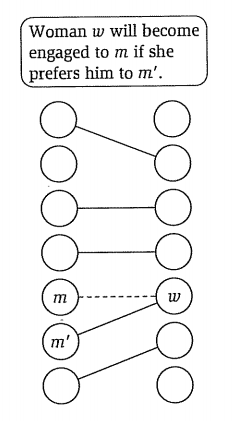
\includegraphics[width=0.25\textwidth]{Imagenes-Seccion2/figura1_2.PNG}
\caption{ Un estado intermedio  del algoritmo G-S cuando un hombre libre $m$ se está proponiendo a una mujer $w$.}
 \label{fig:Imagenes-Seccion2/figura1_2.PNG}
\end{wrapfigure}
   \begin{itemize}
      	\item Inicialmente, todos están solteros. Supongamos que un hombre soltero $m$ elige la mujer $w$ quien está en lo más alto de la lista de preferencias, y se le propone. ¿Inmediatamente podemos declarar que $(m,w)$ será uno de los pares de nuestro emparejamiento estable final? No necesariamente, puede pasar que en el futuro un hombre $m’$ al cual $w$ prefiere se le proponga. Por otro lado, puede ser peligroso para $w$ rechazar a $m$, ya que tal vez nunca reciba una propuesta de alguien que este más arriba en la lista que $m$. Entonces, una idea natural seria que el par $(m,w)$ entre en estado intermedio de compromiso.
\item Supongamos que ahora estamos en un estado en el cual un hombre y una mujer están uno soltero y uno comprometido. El siguiente paso podría verse como este. Un hombre arbitrario soltero $m$ elige la mujer $w$ con la posición más alta en su lista a quien aún no se le propusieron, y él se le propone. Si $w$ esta soltera, entonces $m$ y $w$ se comprometen. De otra manera, $w$ ya está comprometida con otro $m’$. En este caso, ella determina cual $m$ o $m’$ prefiere; el hombre elegido se compromete y el otro queda soltero. 
  \item Finalmente, el algoritmo terminará cuando nadie este soltero; en este momento, todos los compromisos son declarados definitivos, y el resultado es un emparejamiento perfecto. 
    \end{itemize}
    

	Aquí hay una descripción concreta del algoritmo de Gale-Shapley, con la figura \ref{fig:Imagenes-Seccion2/figura1_2.PNG} que representa un estado del algoritmo: $w$ permanece comprometida desde el momento que recibe su primera proposición; y la secuencia de parejas, ira mejorando (en términos de preferencia).
\begin{figure}[h] 
  \centering
    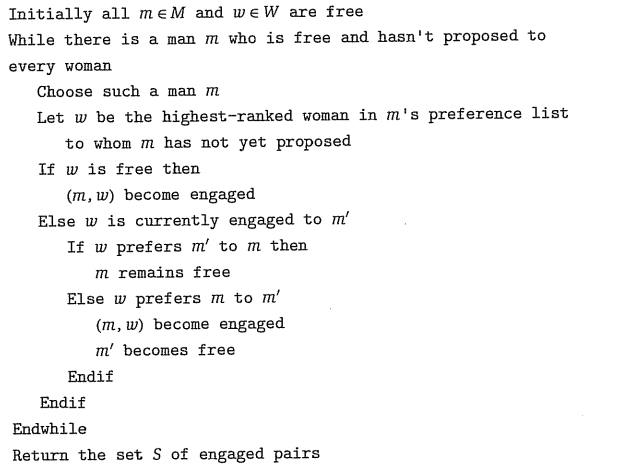
\includegraphics[width=0.7\textwidth]{Imagenes-Seccion2/Imagen1_2.PNG}
\end{figure}

	Algo intrigante es que, aunque el algoritmo G-S es bastante simple de declarar, no es inmediatamente obvio que devuelve una coincidencia estable, o incluso una pareja perfecta. Procedemos a probar esto ahora, a través de una secuencia de hechos intermedios.
\\
\subsubsection*{Analizando el algoritmo}  
Primero consideremos el punto de vista de una mujer durante la ejecución del algoritmo. Por el momento, nadie se le ha propuesto, y  está soletera. Entonces, un hombre puede proponerle matrimonio, y que ella se comprometa. A medida que pasa el tiempo, ella puede recibir propuestas adicionales, aceptando aquellas que vienen de un hombre con mayor preferencia que el actual. De donde descubrimos lo siguiente:
\\
 \\
    \textbf{(1.1) $w$ permanece comprometida desde el momento que recibe su primera proposición; y la secuencia de parejas irá mejorando (en términos de preferencia).}
    \\ 
    \\ 
    El punto de vista de un hombre durante la ejecución del algoritmo, es bastante diferente. Él está soltero hasta que se le propone a la mujer mejor clasificada en su lista; en este punto él puede o no comprometerse. A medida que pasa el tiempo, su estado se puede alterar, entre soltero y comprometido. Sin embargo, la siguiente propiedad se sostiene:
   \\ 
   \\ 
        \textbf{(1.2) La secuencia de mujeres a las que $m$ se le propone, irá empeorando (en términos de preferencia).}
  \\ 
   \\ 
  Ahora mostraremos que el algoritmo termina, y daremos el límite del máximo número de iteraciones necesarias para que finalice.
   \\ 
     \\ 
        \textbf{(1.3)  El algoritmo G-S finaliza después de un máximo de $n^ 2$ iteraciones en el ciclo del While.}
  \\
  \\ 
  \textbf{Demostración:} Una estrategia útil para el  máximo límite de tiempo de ejecución de un algoritmo, es encontrar una medida de progreso. Esto es, buscamos una forma precisa de decir que cada paso dado por el algoritmo lo lleva más cerca de la finalización.
  En el caso del algoritmo actual, cada iteración consiste en que un hombre se le propone (por una sola vez) a una mujer, a la que nunca se le ha propuesto. Entonces, si denotamos al conjunto de pares $(m, w)$ como $P(t)$, tal que $m$ se le ha propuesto a $w$ al final de la iteración $t$, vemos que para todo t el tamaño de $P(t+1)$ es estrictamente mayor que el tamaño de $P(t)$. Pero solo hay $n \times n$ posibles pares de hombres y mujeres en total; entonces, el valor de $P(.)$ puedo aumentar como mucho $n^ 2$ veces en el transcurso del algoritmo. Se deduce que puede haber como máximo $n^ 2$ iteraciones. 
  \\ 
  \\ 
  	Vale la pena destacar dos puntos sobre el hecho anterior y su prueba. Primero, hay ejecuciones del algoritmo (con ciertas listas de preferencias) que pueden implicar cerca de $n^ 2$ iteraciones, por lo que este análisis no está lejos de ser el mejor posible.
      \\
    
En segundo lugar, hay muchas cantidades que no habrían funcionado correctamente como medida de progreso Para el para el algoritmo, ya que no es necesario un incremento en cada iteración. Por ejemplo, el número de individuos solteros podría permanecer constante de una iteración a la siguiente, al igual que el número de pares comprometidos. Así, estas cantidades no pueden usarse directamente para dar un cota superior en el número máximo posible de iteraciones, con respecto al párrafo anterior.   \\

Vamos a establecer que el conjunto $S$ devuelto de la finalización del algoritmo, es de hecho, un emparejamiento perfecto. ¿Por qué esto no es inmediatamente obvio? Esencialmente, tenemos que mostrar que ningún un hombre puede “caer” al final de su lista de preferencias, la única forma de salir del ciclo while , es que no haya ningún hombre soltero. En este caso, el conjunto de parejas comprometidas seria en efecto, un emparejamiento perfecto. \\ 

Entonces, lo principal que tenemos que mostrar es lo siguiente:
  \\ 
  \\
    \textbf{(1.4) Sí $m$ esta soltero en algún punto de la ejecución del algoritmo, entonces hay una mujer a la que aún no se le ha propuesto.
 }
    \\
      \\ 
  \textbf{Demostración:} Supongamos que se llega al punto en que $m$ esta soltero, pero ya se le propuso a todas las mujeres. Luego, por (1.1), cada una de las $n$ mujeres esta comprometida en este momento. Dado que el conjunto de pares comprometidos forma un emparejamiento, también debe haber $n$ hombres comprometidos. Pero solo hay $n$ hombres en total, y $m$ no esta comprometido, con lo cual se llega a una contradicción. 
  \\ 
 \\
    \textbf{(1.5) El conjunto devuelto $S$ es un emparejamiento 		perfecto}
    \\ \\
    \textbf{Demostración:} El conjunto de pares comprometidos siempre forma un emparejamiento. Supongamos que el algoritmo termina con un hombre $m$ libre. Al finalizar, este debe ser el caso en que $m$ se propuso a todas las mujeres, ya que sino el ciclo while no hubiera terminado. Sin embargo esto contradice (1.4), que dice que no puede haber un hombre libre luego de haberse propuesto a todas las mujeres.
 \\ \\
 Finalmente probamos la propiedad principal del algoritmo, es decir, que resulta en un emparejamiento estable.\\ \\
 \colorbox{mygray}{\parbox{15cm}{
\textbf{(1.6) Consideremos una ejecución del algoritmo G-S, que devuelve un conjunto S de pares. El conjunto S es un emparejamiento estable.}}}\\
      \\ \\
   \textbf{Demostración:} Ya vimos en (1.5), que $S$ es un emparejamiento perfecto. De esta forma, para probar que S es un emparejamiento estable, asumiremos que hay una inestabilidad con respecto a $S$, y obtener una contradicción. Como definimos anteriormente, dicha inestabilidad abarca dos pares, $(m,w)$ y $(m’,w’)$, en $S$, con las propiedades que:
  \\
   \begin{itemize}
      \item $m$ prefiere a $w’$ antes que a $w$ 
      \item $w’$ prefiere a $m$ antes que a $m’$
    \end{itemize}
En la ejecución del algoritmo que genera a $S$, la ultima proposición de $m’$ fue, por definición, a $w$. Ahora nos preguntamos, ¿$m$ le propuso a $w’$ en algún punto anterior en esta ejecución? Si no lo hizo, entonces $w$ está más adelante en la lista de preferencias de $m$, contradiciendo nuestra suposición de que $m$ prefiere a $w’$ antes que a $w$. Si lo hizo, entonces $m$ fue rechazado por $w$, a favor de otro hombre $m_1$, a quien $w$ prefiere antes que a $m$; $m’$ es la pareja final de $w’$, entonces, o $m’$ = $m_1$, o por (1.1), $w’$ prefiere a $m’$ antes que a $m’$. Cualquieras de estas dos situaciones contradice nuestra suposición de que $w’$ prefiere a $m$ antes que a $m’$.Luego, S es un emparejamiento estable.    $ \blacksquare $ 
\subparagraph{EXTENSIONES} ~\\

Comenzamos definiendo la noción de emparejamiento estable; hemos probado que el algoritmo G-S  construye uno. Ahora consideramos alguna  otra cuestión sobre el comportamiento del algoritmo G-S y su relación con las propiedades de diferentes emparejamientos estables.\\

Para comenzar, recordemos que vimos un ejemplo anteriormente en el cual se podían dar múltiples emparejamientos estables. En este caso, la lista de preferencias era la siguiente:	
\begin{itemize}
  \item $m$ prefiere a $w$ antes que a $w'$
  \item $m'$ prefiere a $w'$ antes que a $w$
  \item $w$ prefiere a $m'$ antes que a $m$
  \item $w'$ prefiere $m$ antes que $m'$
\end{itemize}
Ahora en cualquier ejecución del algoritmo, $m$ estará emparejado con $w$, $m’$ estará emparejado con $w’$ (quizás en otro orden), y todo terminaría ahi. Así, el otro emparejamiento estable, que consiste en los pares $(m’,w)$ y $(m,w’)$, no es alcanzable en una ejecución del algoritmo en el que el hombre propone. Por otro lado, si sería posible lograrlo si ejecutaremos una versión modificada del algoritmo, en el cual las mujeres propusieran. Y en ejemplos más grande, con más de dos personas de cada lado, podríamos tener una gran colección posible de emparejamientos estables, muchos de ellos no pudiendo ser obtenidos por un algoritmo natural.
\\
\\
Este ejemplo muestra una cierta “injusticia” en el algoritmo G-S, favoreciendo a los hombres. Si las preferencias de ellos engranaran perfectamente (todos listan diferentes mujeres como su primera preferencia), entonces en todas las ejecuciones del algoritmo, todos los hombres terminarían emparejados con su primera elección, independientemente de las elecciones de las mujeres. Si las preferencias de las mujeres chocaran con las preferencias de los hombres (como pasó en el ejemplo), entonces el resultado sería tan malo como es posible para las mujeres. Entonces este simple conjunto de preferencias resume claramente un mundo donde alguien está destinado a terminar insatisfecho; las mujeres están insatisfechas si los hombres propone, y los hombres están insatisfechos si las mujeres proponen.
\\
\\
Analicemos más en detalle el algoritmo y veamos que tan general esta “injusticia” es.
\\
\\
Para comenzar, nuestro ejemplo refuerza el punto en que el algoritmo G-S aún no está especificado: tan pronto como haya un hombre libre, tendremos la posibilidad de elegir cualquier hombre libre para hacer la siguiente proposición. Diferentes elecciones especifican diferentes ejecuciones del algoritmo; esta es la razón, para tener cuidado, fijamos (1.6) como “Consideremos una ejecución del algoritmo G-S, que devuelve un conjunto S de pares.” en lugar de “Consideremos el conjunto S devuelto por el algoritmo G-S”.
\\
\\
Así encontramos otra pregunta muy natural: ¿Todas las ejecuciones del algoritmo resultan en el mismo emparejamiento? Esta es una pregunta genérica, que surge en muchos escenarios en Ciencias de la Computación: tenemos un algoritmo que corre asíncronamente, con distintos componentes independientes, que realizan acciones que pueden ser intercaladas en formás complejas, y queremos saber que tanta variación genera esta asincronía en el resultado final. Para considerar un ejemplo muy distinto, los componentes independientes pueden ser componentes electrónicos activando partes del ala de un avión; el efecto de asincronía en su comportamiento puede ser un gran problema.\\

En el presente contexto, veremos que la respuesta a nuestra pregunta es sorprendentemente clara: toda ejecución del algoritmo G-S rinden el mismo emparejamiento. Procedamos a probar esto ahora.\\

\textbf{Todas las ejecuciones producen el mismo ajuste.}
Hay varias maneras posibles de probar una afirmación como esta, muchas de las cuales resultarían en argumentos bastante complicados. Resulta que el enfoque más fácil y más informativo para nosotros será caracterizar de forma única la coincidencia que se obtiene y luego mostrar que todas las ejecuciones dan como resultado el emparejamiento con esta caracterización.
¿Cuál es la caracterización? Mostraremos que cada hombre termina con la "mejor pareja posible" en un sentido concreto. (Recuerde que esto es cierto si todos los hombres prefieren mujeres diferentes). Primero, diremos que una mujer $w$ es una pareja válida de un hombre $m$ si hay una pareja estable que contiene el par $(m, w)$. Diremos que $w$ es la mejor pareja válida de $m$ si $w$ es una pareja válida de $m$, y ninguna mujer con un rango $m$ superior a $w$ es una pareja válida de $m$. Utilizaremos el mejor $(m)$ para denotar la mejor pareja válida de $m$. Ahora, deje que $S*$ denote el conjunto de pares ${(m, mejor (m)): m  \in  M}$. Vamos a probar el siguiente hecho\\ \\\\
 \colorbox{mygray}{\parbox{15cm}{
\textbf{(1.7) Cada ejecución del algoritmo $G-S$ da como resultado el conjunto $S*$.}}}\\
      \\
      
Esta afirmación es sorprendente en varios niveles. En primer lugar, tal como se define, no hay ninguna razón para creer que $S*$ sea un emparejamiento en absoluto, y mucho menos un emparejamiento estable. Después de todo, ¿por qué no podría suceder que dos hombres tuvieran la misma mejor pareja válida? En segundo lugar, el resultado muestra que el algoritmo $G-S$ brinda el mejor resultado posible para cada hombre simultáneamente; no hay una coincidencia estable en la que ninguno de los hombres podría haber esperado hacerlo mejor. Y finalmente, responde a nuestra pregunta anterior mostrando que el orden de las propuestas en el algoritmo $G-S$ no tiene ningún efecto en el resultado final.\\

A pesar de todo esto, la prueba no es tan difícil.\\

\textbf{Demostración}. Supongamos, a modo de contradicción, que alguna ejecución $E$ del algoritmo $G-S$ resulta en una $S$ correspondiente en la que un hombre se empareja con una mujer que no es su mejor compañero válido. Como los hombres proponen en orden decreciente de preferencia, esto significa que un hombre es rechazado por una compañera válida durante la ejecución $E$ del algoritmo. Así que considere el primer momento durante la ejecución $E$ en el que un hombre, digamos $m$, es rechazado por una pareja válida $w$. De nuevo, dado que los hombres proponen en orden decreciente de preferencia, y dado que esta es la primera vez que se produce dicho rechazo, debe ser que $w$ sea la mejor pareja válida de $m$.\\

El rechazo de $m$ por $w$ puede haber ocurrido porque $m$ propuso y fue rechazado a favor del compromiso existente de $w$, o porque $w$ rompió su compromiso a favor de una mejor propuesta. Pero de cualquier manera, en este momento, $w$ forma o continúa un compromiso con un hombre que desea recibir $m$.\\

Como $w$ es una pareja válida de $m$, existe un $S_1$ de coincidencia estable que contiene el par $(m, w)$. Ahora preguntamos: ¿con quién estoy emparejado en este emparejamiento? Supongamos que es una mujer $w'≠ w$.\\

Dado que el rechazo de $m$ por $w$ fue el primer rechazo de un hombre por una pareja válida en la ejecución $E$, debe ser que $m'$ no haya sido enredado por ninguna pareja válida en el punto $E$ cuando se comprometió con $w$. Como propuso en orden decreciente de preferencia, y como $w'$ es claramente una pareja válida de $m'$, debe ser que $m'$ prefiera $w$ antes que a $w'$. Pero ya hemos visto que $w$ prefiere $m'$ antes que a $m$, porque en ejecución de $E$ rechazó a $m$ a favor de $m'$. ¿Desde $ (m',w) ∉ S$?, se deduce que $(m', w)$ es una inestabilidad en $S'$ .Esto contradice nuestra afirmación de que $S'$ es estable y por lo tanto contradice nuestra inicial suposición.
$ \blacksquare $\\

Supongamos que hay un par $(m, w)$ en $S*$ tal que $m$ no es la peor pareja válida de $w$. Luego hay un $S*$ que se corresponde estable en el que $w$ está emparejado\\

Entonces, para los hombres, el algoritmo $G-S$ es ideal. Desafortunadamente, no se puede decir lo mismo de las mujeres. Para una mujer $w$, decimos que $m$ es una pareja válida si hay una coincidencia estable que contiene el par $(m, w)$. Decimos que $m$ es la peor pareja válida de $w$ si $m$ es una pareja válida de $w$, y ningún hombre con rango inferior a $m$ es una pareja válida de ella.\\

$(1.8)$ En el conjunto $S*$, cada mujer está emparejada con su peor pareja válida.\\

\textbf{Demostración}. Supongamos que hay un par $(m, w)$ en $S*$ tal que $m$ no es la peor pareja válida de $w$. Luego hay una $S'$ que se corresponde estable en la que $w$ se empareja con un hombre $m'$ que le gusta menos que $m$. En $S'$ , $m$ está emparejado con una mujer $w'≠ w$; ya que $w$ es la mejor pareja válida de $m$, y $w'$ es una pareja válida de $m$, vemos que $m$ prefiere $w$ a $w'$.\\

Pero de esto se deduce que $(m, w)$ es una inestabilidad en $S'$, lo que contradice la afirmación de que $S'$ es estable y, por lo tanto, contradice nuestra suposición inicial.$ \blacksquare $\\

Por lo tanto, encontramos que nuestro simple ejemplo anterior, en el que las preferencias de los hombres chocaban con las mujeres, insinuaba un fenómeno muy general: para cualquier entrada, el lado que hace la proposición en el algoritmo $G-S$ termina con la mejor coincidencia estable posible (desde su perspectiva), mientras que el lado que no hace la proposición en consecuencia termina con el peor ajuste estable posible.\\

\subsection{Cinco Problemás Representativos}

El Problema de Emparejamiento Estable nos brinda un rico ejemplo del proceso de diseño de algoritmos. Para muchos problemás, este proceso involucra algunos pasos significantes: formular el problema con la suficiente precisión matemática con la que podemos formularnos una pregunta concreta y comenzar a pensar sobre los algoritmos para resolverla; diseñando un algoritmo para el problema; y analizando el algoritmo, probando que es correcto y dando un límite en el tiempo de ejecución, de forma que podamos establecer la eficiencia de dicho algoritmo.
\\
\\
Esta estrategia de alto nivel, es llevada a la práctica con la ayuda de unas pocas, pero fundamentales, técnicas de diseño, las cuales son muy útiles a la hora de evaluar la inherente complejidad de un problema, y de formular un algoritmo para resolverlo. Como en cualquier área, familiarizarse con estas técnicas es un proceso gradual; pero con experiencia, uno puede empezar a reconocer problemás como pertenecer a géneros identificables, y apreciando como pequeños cambios en el enunciado de un problema pueden tener un enorme efecto en la dificultad computacional de este.
\\
\\
Para comenzar esta discusión, es de ayuda elegir algunos hechos representativos que encontraremos en nuestro estudio de los algoritmos: problemás claramente formulados,  todos similares entre si a un nivel general, pero diferentes en su dificultad y en los tipos de  enfoque que cada uno le da. Los primeros tres serán resolubles eficientemente por una secuencia de crecientes y sutiles técnica de algoritmos; y el quinto aluda a una clase de problemás que se cree que es aún más difícil.
\\
\\
Los problemás son independientes y todos motivados por aplicaciones en la informática. Para hablar sobre algunos de ellos, sin embargo, será de ayuda el uso de la terminología de Grafos. Aunque los grafos son un tema común en cursos iniciales de ciencias de la computación, los estaremos introduciendo muy profundamente en el Capítulo 3, debido a su enorme poder expresivo, que lo usaremos ampliamente a lo largo de este libro. Para esta discusión, es suficiente pensar en un grafo G como una simple forma de codificar relaciones de parejas como un conjunto de objetos. De esta forma, G consiste en un par de conjuntos (V , E) -una colección V de nodos y una colección E de aristas, cada uno de los cuales une dos nodos. Así representamos un arista $e $ $ \epsilon $ E como un subconjunto de dos elementos de V: $e = \{  u,v \}$ para algún u,v $\epsilon$ V, donde llamamos a u y a v los extremos de e. Típicamente dibujamos grafos como en la Figura 2, con cada nodo como un pequeño círculo y cada arista como un segmento que une sus dos extremos.
\\
\\
Empecemos ahora la discusión sobre los cinco problemás representativos.\\

\begin{wrapfigure}{t}{0.2\textwidth}
\centering
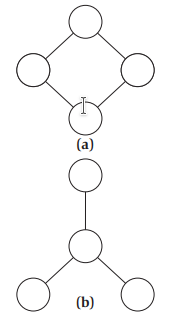
\includegraphics[width=0.19\textwidth]{Imagenes-Seccion1/fig1_3.png}
\caption{Tanto (a) como (b) representan un grafo de cuatro nodos}
\end{wrapfigure}

\subsubsection*{Planificación de tareas en intervalos}

Considere el siguiente problema de planificación muy simple. Usted tiene un recurso, puede ser una sala de conferencias, una supercomputadora o un microscopio electrónico, y muchas personas solicitan utilizar el recurso durante períodos de tiempo. Una solicitud toma la forma: ¿Puedo reservar el recurso comenzando en el tiempo $s$, hasta el momento $f$? Asumiremos que el recurso puede ser utilizado por, como máximo, una persona a la vez. Un planificador desea aceptar un subconjunto de estas solicitudes, rechazando todas las demás, de modo que las solicitudes aceptadas no se superpongan en el tiempo. El objetivo es maximizar la cantidad de solicitudes aceptadas.\\

Más formalmente, habrá $n$ solicitudes etiquetadas como $1, ..., n$, con cada solicitud que especifique una hora de inicio $s_i$ y un tiempo de finalización $f_i$. Naturalmente, tenemos $s_i<f_i$ para todo $i$. Dos solicitudes $i$ y $j$ son compatibles si los intervalos solicitados no se superponen: es decir, o la solicitud $i$ es para un intervalo de tiempo anterior a la solicitud $j$ ($f_i≤s_j$), o la solicitud $i$ es para un momento posterior a la solicitud $j$ ($f_j≤s_i$). En general, diremos que un subconjunto $A$ de solicitudes es compatible si todos los pares de solicitudes $i$, $j  \in  A$, $i≠J$ son compatibles. El objetivo es seleccionar un subconjunto compatible de solicitudes del tamaño máximo posible.\\

Ilustramos una instancia de este problema de planificación de intervalos en la figura. Tenga en cuenta que hay un único conjunto compatible de tamaño 4, y este es el conjunto compatible más grande.\\


\begin{figure}[h]
\centering
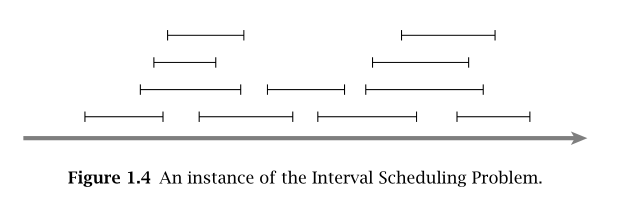
\includegraphics[scale=0.7]{Imagenes-Seccion1/fig1-4.PNG}
\end{figure}


Veremos en breve que este problema puede resolverse mediante un algoritmo muy natural que ordena el conjunto de solicitudes de acuerdo con una cierta heurística y luego las procesa con "avidez" en una pasada, seleccionando un subconjunto compatible tan grande como sea posible. Esto será típico de una clase de algoritmos ávidos que consideraremos para varios problemás: reglas de corto alcance que procesan la entrada de una pieza a la vez sin aparente anticipación. Cuando se puede mostrar un algoritmo ávido para encontrar una solución óptima para todas las instancias de un problema, a menudo es bastante sorprendente. Normalmente aprendemos algo sobre la estructura del problema subyacente por el hecho de que un enfoque tan simple puede ser óptimo.\\

\subsubsection*{Planificación de Intervalos Ponderados}

En el Problema de Planificación de Intervalos, buscamos maximizar el número de solicitudes que pueden ser acomodadas simultáneamente. Ahora supongamos de forma más general que cada intervalo de solicitud $i$ tiene un valor asociado, o $peso$, $v_i > 0$. Podemos representar esto como la cantidad de dinero que haremos por el $i-ésimo$ individuo, si prlanificamos su solicitud. Nuestra meta será encontrar un subconjunto compatible de intervalos de máximo valor total.
\\\\
El caso en el que $v_i = 1$ para cada $i$ es simplemente el Problema de Planificación de Intervalos; pero la aparición de cambios arbitrarios de valores, cambian bastante la naturaleza del problema. Consideremos por ejemplo, que si $v_1$ pasa la suma de todos los $v_i$, entonces la solución del problema puede incluir intervalos 1, independientemente de la configuración del conjunto completo de intervalos. De esta forma, cualquier algoritmo para este problema debe ser muy sensible a los valores, y todavía degenerada a la forma de resolver el problema de planificación de intervalos, cuando todos los valores son iguales a 1.
\\\\
Entonces parece ser, no simplemente reglas ávidas que caminan a través de intervalos, uno a la vez, tomando las decisiones correctas en la presencias de valores arbitrarios. En lugar de esto, empleamos una técnica $programación$ $dinámica$ que construye el valor óptimo sobre todas las posibles soluciones en un compacto, forma tabular que conduce a un algoritmo muy eficiente.\\

\subsubsection*{Emparejamiento Bipartito}

Cuando consideramos el Problema de Emparejamiento Estable, definimos emparejamiento como un conjunto de pares ordenados de hombres y mujeres, con las propiedades de que cada hombre y cada mujer pertenecen como máximo a un par.\\\\
Podemos expresar estos conceptos de forma más general, en términos de grafos, y para hacerlo, es útil definir la noción de grafo bipartito. Decimos que un grafo $G = (V,E)$ es $bipartito$ si su conjunto de nodos $V$ puede ser dividido en conjuntos $X$ e $Y$ de forma tal que cada arista tiene un final en $X$ y el otro final en $Y$. Un grafo bipartito está representado en la figura 2.5; usualmente, cuando queremos enfatizar en la "bipartidad" de un grafo, lo dibujaremos de esta forma, con los nodos en $X$ y en $Y$ en columnas paralelas. Pero hay que notar que, por ejemplo, que los dos grafos en la figura 2 también son bipartitos.\\\\

\begin{wrapfigure}{t}{0.2\textwidth}
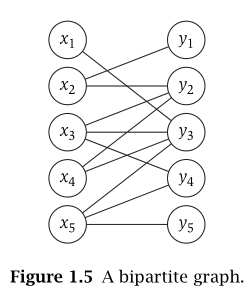
\includegraphics[width=0.25\textwidth]{Imagenes-Seccion1/fig1-5.PNG}
\caption{ Fig 1.5}
 \label{fig:Imagenes-Seccion1/fig1-5.PNG}
\end{wrapfigure}

Ahora, en el problema de encontrar un emparejamiento estable, los emparejamientos fueron construidos a partir de pares de hombres y mujeres. En el caso de los grafos bipartitos, las aristas son pares de nodos, por lo cual decimos que un emparejamiento en un grafo $G = (V,E)$ es un conjunto de aristas $M \subset E$ con la propiedad de que cada nodo aparece como máximo en un arista de $M$. $M$ es un emparejamiento estable si cada nodo aparece exactamente en un arista de M.
\\\\
Para ver que esto tiene la misma esencia que el Problema de Emparejamiento Estable, consideremos un grafo bipartito $G'$, con un conjunto $X$ de $n$ hombres, un conjunto $Y$ de $n$ mujeres, y un arista desde cada nodo en $X$ a cada nodo en $Y$. Entonces los emparejamientos, y los emparejamientos perfectos en $G'$ son precisamente los emparejamientos y emparejamientos perfectos sobre el conjunto de hombres y mujeres.
\\\\
En el Problema de Emparejamiento Estable añadimos preferencias a esta representación. Acá no consideramos preferencias; pero la naturaleza del problema en grafos bipartitos arbitrarios agrega una fuente distinta de complejidad: no hay necesariamente un arista desde cada $x \in X$ a cada $y \in Y$ , entonces el conjunto de posibles emparejamientos tiene una estructura un poco más complicada. En otras palabras es que solamente algunos pares de hombres y mujeres están dispuestos a ser emparejados, y queremos darnos cuenta como emparejar muchas personas de forma que sea consistente con esto. Consideremos por ejemplo, el grafo bipartito $G$ de la figura 2.5: hay muchos emparejamientos en $G$, pero solamente un emparejamiento perfecto (¿Puedes verlo?).
\\\\
Emparejamiento en grafos bipartitos pueden modelar situaciones en las que objetos son asignados a otros objetos. Así, los nodos en $X$ pueden representar trabajos, los nodos en $Y$ pueden representar máquinas, y un arista $(x_i,y_i)$ puede indicar que la máquina $y_i$ puede hacer el trabajo $x_i$. Un emparejamiento perfecto es entonces una forma de asignar cada trabajo a una máquina que pueda realizarlo, con la propiedad de que cada máquina está asignada exactamente a un trabajo. También, los departamentos de ciencias de la computación, pueden ser representados como grafos bipartitos, con $X$ el conjunto de profesores en el departamento, $Y$ el conjunto de cursos ofrecidos, y cada arista $(x_i, y_i)$ indica que el profesor $x_i$ es capaz de enseñar el curso $y_i$. Un emparejamiento perfecto consiste en asignar cada profesor a un curso que puede enseñar, de forma que cada curso sea cubierto.
\\\\
Así el Emparejamiento Bipartito es el siguiente: Dado un grafo bipartito y arbitrario $G$, encontrar un emparejamiento de tamaño máximo. Si $|X| = |Y| = n$ entonces hay un emparejamiento perfecto si y solamente si el máximo emparejamiento tiene tamaño $n$. Encontraremos que las técnicas algorítmicas discutidas anteriormente no se ven adecuadas parar proveer un algoritmo eficiente para este problema. Sin embargo, existe un muy elegante y eficiente algoritmo para encontrar el máximo emparejamiento: se construye inductivamente sobre cada vez más grandes emparejamientos, retrocediendo selectivamente sobre el camino. Este proceso es llamado $"aumento"$ y conforma el elemento central en una gran clase de problemás resolubles eficientemente llamados "network flow problems" (problemás de flujo de red).\\

\subsubsection*{Conjunto independiente}

Ahora hablemos de un problema extremadamente general, que incluye la mayoría de estos problemás anteriores como casos especiales. Dado un grafo $G=(V,E)$, diga que un conjunto de odas $S⊆V$ es independiente si no hay dos nodos en $S$ unidos por un arista. El problema del conjunto independiente es, entonces, el siguiente: dada $G$, encuentre un conjunto independiente que sea lo más grande posible. Por ejemplo, el tamaño máximo de un conjunto independiente en el grafo de la Figura 1.6 es cuatro, logrado por el conjunto independiente de cuatro nodos ${1,4,5,6}$.\\

\begin{wrapfigure}{t}{0.2\textwidth}
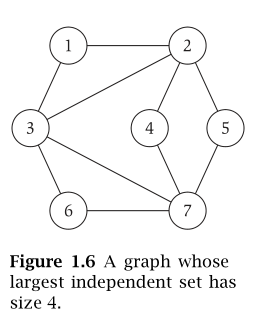
\includegraphics[width=0.25\textwidth]{Imagenes-Seccion1/fig1-6.PNG}
\caption{ Fig 1.6}
 \label{fig:Imagenes-Seccion1/fig1-6.PNG}
\end{wrapfigure}

El problema del conjunto independiente codifica cualquier situación en la que intente elegir entre una colección de objetos y existen conflictos por pares entre algunos de los objetos. Digamos que tiene $n$ amigos, y algunos pares de ellos no se llevan bien. ¿Qué tan grande puede invitar a cenar a un grupo de amigos si no quieres tensiones interpersonales? Este es simplemente el conjunto independiente más grande en el grafo cuyos nodos son tus amigos, con una ventaja entre cada par en conflicto.\\

La Planificación por intervalos y la Igualación bipartita pueden codificarse como casos especiales del Problema del conjunto independiente. Para la planificación por intervalos, defina un grafo $G=(V,E)$ en el cual los nodos son los intervalos y hay un arista entre cada par de ellos que se superponen; los conjuntos independientes en $G$ son entonces solo los subconjuntos de intervalos compatibles. Codificando el emparejamiento bipartito como un caso especial de Independent Set es un poco más complicado de ver. Dado un grafo bipartito $G'=(V',E')$, los objetos que se eligen son aristas, y los conflictos surgen entre dos aristas que comparten un extremo. (Estos, de hecho, son los pares de aristas que no pueden pertenecer a una coincidencia común). Por lo tanto, definimos un grafo $G=(V,E)$ en el que el conjunto de nodos V es igual al conjunto de aristas $E'$ de $G'$. Definimos un aristas entre cada par de elementos en V que corresponden a las aristas de $G'$ con un extremo común. Ahora podemos verificar que los conjuntos independientes de $G$ son precisamente los emparejamientos de $G'$. Si bien no es complicado verificar esto, se necesita un poco de concentración para manejar este tipo de transformación de "aristas a nodos, nodos a aristas".\\

Dada la generalidad del problema del conjunto independiente, un algoritmo eficiente para resolverlo sería bastante impresionante. Tendría que contener implícitamente algoritmos para planificación por intervalos, emparejamiento bipartito y una serie de otros problemás naturales de optimización.\\

El estado actual del conjunto independiente es este: no se conoce ningún algoritmo eficiente para el problema, y se conjetura que no existe dicho algoritmo. El obvio algoritmo de fuerza bruta probaría todos los subconjuntos de los nodos, verificando cada uno para ver si es independiente y luego registrando el más grande encontrado. Es posible que esto esté cerca de lo mejor que podemos hacer con este problema. Veremos más adelante en el libro que el Conjunto independiente es uno de una gran clase de problemás que se denominan NP completos. No se conoce ningún algoritmo eficiente para ninguno de ellos; pero todos son equivalentes en el sentido de que una solución a cualquiera de ellos implicaría, en un sentido preciso, una solución para todos ellos.\\

Aquí hay una pregunta natural: ¿hay algo bueno que podamos decir sobre la complejidad del problema del conjunto independiente? Una cosa positiva es la siguiente: si tenemos un grafo $G$ en 1,000 nodos, y queremos convencerlo de que contiene un conjunto independiente $S$ del tamaño 100, entonces es bastante fácil. Simplemente le mostramos el grafo $G$, rodeamos los nodos de $S$ en rojo y le permitimos comprobar que no hay dos de ellos unidos por un arista. Entonces, realmente parece haber una gran diferencia en la dificultad entre verificar que algo es un gran conjunto independiente y, en realidad, encontrar un gran conjunto independiente. Esto puede parecer una observación muy básica, y lo es, pero resulta crucial para comprender esta clase de problemás. Además, como veremos a continuación, es posible que un problema sea tan difícil que ni siquiera haya una manera fácil de "verificar" las soluciones en este sentido.\\

\subsubsection*{Ubicación de instalaciones competitivas}

Finalmente, llegamos a nuestro quinto problema, que se basa en el siguiente juego de dos jugadores. Considere dos grandes compañías que operan franquicias de cafés en todo el país, llamémoslas JavaPlanet y Queequeg's Coffee, y actualmente compiten por una participación de mercado en un área geográfica. Primero JavaPlanet abre una franquicia; luego Queequeg's Coffee abre una franquicia; luego JavaPlanet; luego el de Queequeg; y así. Supongamos que deben lidiar con las reglamentaciones de zonificación que requieren que no haya dos franquicias ubicadas muy juntas, y cada una intenta hacer que su ubicación sea lo más conveniente posible. ¿Quién ganará?\\

\begin{figure}[h]
\centering
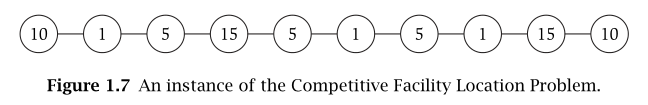
\includegraphics[scale=0.83]{Imagenes-Seccion1/fig1-7.PNG}
\end{figure}

Hagamos las reglas de este "juego" más concretas. La región geográfica en cuestión se divide en $n$ zonas, etiquetadas $1, 2,. . . ,n$. Cada zona $i$ tiene un valor $bi$, que es el ingreso obtenido por cualquiera de las compañías si abre una franquicia allí. Finalmente, ciertos pares de zonas $(i,j)$ son adyacentes, y las leyes de zonificación locales previenen que dos zonas adyacentes de cada una contengan una franquicia, independientemente de la compañía que las posea. (También evitan que se abran dos franquicias en la misma zona.) Modelamos estos conflictos mediante un grafo $G=(V,E)$, donde $V$ es el conjunto de zonas, y $(i,j)$ es un arista en $E$ si las zonas $i$ y $j$ son adyacentes. El requisito de zonificación dice que el conjunto completo de franquicias abiertas debe formar un conjunto independiente en $G$.\\

Por lo tanto, nuestro juego consiste en dos jugadores, $P1$ y $P2$, que seleccionan nodos alternativamente en $G$, y $P1$ se mueve primero. En todo momento, el conjunto de todos los nodos seleccionados debe formar un conjunto independiente en $G$. Supongamos que el jugador $P2$ tiene un objetivo enlazado $B$, y queremos saber: ¿existe una estrategia para $P2$ de modo que no importa cómo se reproduzca $P1$, $P2$ ser capaz de seleccionar un conjunto de nodos con un valor total de al menos $B$? Llamaremos a esto una instancia del problema de ubicación de instalaciones competitivas.\\

Considere, por ejemplo, la instancia representada en la Figura 1.7, y suponga que el objetivo de $P2$ es $B=20$. Entonces $P2$ tiene una estrategia ganadora. Por otro lado, si $B=25$, entonces $P2$ no lo hace.\\

Uno puede resolver esto mirando la figura por un tiempo; pero requiere cierta cantidad de verificación de casos del formulario, "Si $P1$ va aquí, entonces $P2$ irá allí; pero si $P1$ va allí, entonces $P2$ irá aquí ... "Y esto parece ser intrínseco al problema: no solo es computacionalmente difícil determinar si $P2$ tiene una estrategia ganadora; en un grafo de un tamaño razonable, incluso sería difícil para nosotros convencerlo de que $P2$ tiene una estrategia ganadora. No parece haber una pequeña prueba que podamos presentar; más bien, tendríamos que guiarlo en un largo análisis caso por caso del conjunto de posibles movimientos.\\

Esto está en contraste con el problema del conjunto independiente, donde creemos que encontrar una solución grande es difícil, pero es fácil verificar una gran solución propuesta. Este contraste se puede formalizar en la clase de problemás PSPACE-completo, de los cuales la Ubicación de instalaciones competitivas es un ejemplo. Se cree que los problemás PSPACE-completo son estrictamente más difíciles que los problemás NP-completo, y esta conjeturada falta de "pruebas" breves para sus soluciones es una indicación de esta mayor dureza. La noción de PSPACE-completeness resulta para capturar una gran colección de problemás que involucran juegos y planificación; muchos de estos son problemás fundamentales en el área de la inteligencia artificial.\\

\subsection{Ejercicios Resueltos}

\subsubsection*{Ejercicio 1}

Considera un pueblo con $n$ hombres y mujeres que buscan casarse el uno con el otro. Cada hombre tiene una lista de preferencias que clasifica a todas las mujeres, y cada mujer tiene una lista de preferencias que clasifica a todos los hombres.\\

El conjunto de todas las personas $2n$ se divide en dos categorías: buenas personas y malas personas. Supongamos que para algún número $k$, $1≤k≤n-1$, hay $k$ hombres buenos y $k$ mujeres buenas; por lo tanto, hay $n-k$ malos hombres y $n-k$ malas mujeres.\\

Todos preferirían casarse con cualquier persona buena que cualquier mala persona. Formalmente, cada lista de preferencias tiene la propiedad de que clasifica a cada persona buena del género opuesto más alta que cada persona mala del género opuesto: sus primeras $k$ entradas son las buenas personas (del género opuesto) en algún orden, y su siguiente $n-k$ son las personas malas (del sexo opuesto) en algún orden.\\

Demuestre que en cada emparejamiento estable, todo buen hombre está casado con una buena mujer.\\

\textbf{Solución} Una forma natural de empezar a pensar sobre este problema es suponer que el reclamo es falso y tratar de trabajar para obtener una contradicción. ¿Qué significaría que el reclamo sea falso? Existiría un apareamiento estable $M$ en el que un buen hombre estaba casado con una mala mujer $w$.\\

Ahora, consideremos qué aspecto tienen los otros pares en $M$. Hay $k$ buenos hombres y $k$ buenas mujeres. ¿Podría ser el caso que cada buena mujer está casada con un buen hombre en este $M$? No: uno de los hombres buenos (es decir, $m$) ya está casado con una mujer mala, y eso deja solo a otros $k-1$ hombres buenos. Entonces, aunque todos ellos estuvieran casados con mujeres buenas, eso dejaría a una mujer buena que está casada con un hombre malo.\\

Vamos a ser una mujer tan buena, que está casada con un hombre malo. Ahora es fácil identificar una inestabilidad en $M$: considere el par $(m,w')$. Cada uno es bueno, pero está casado con un mal compañero. Por lo tanto, cada uno de $m$ y $w'$ prefiere el otro a su compañero actual, y por lo tanto $(m,w')$ es una inestabilidad. Esto contradice nuestra suposición de que $M$ es estable y, por lo tanto, concluye la prueba.\\

\subsubsection*{Ejercicio 2}

Podemos pensar en una generalización del problema de apareamiento estable en el que ciertos pares hombre-mujer están explícitamente prohibidos. En el caso de los empleadores y solicitantes, podríamos imaginar que ciertos solicitantes simplemente carecen de las calificaciones o certificaciones necesarias, por lo que no pueden ser empleados en ciertas empresas, por más deseables que parezcan. Utilizando la analogía para el matrimonio entre hombres y mujeres, tenemos un conjunto $M$ de $n$ hombres, un conjunto $W$ de $n$ mujeres, y un conjunto $F⊆M×W$ de parejas que simplemente no pueden casarse. Cada hombre $m$ clasifica todas las mujeres $w$ para las cuales $(m,w)∉F$, y cada mujer $w'$ clasifica a todos los hombres $m'$ para los cuales $(m',w')∉F$. En este contexto más general, decimos que un $S$ correspondiente es estable si no presenta ninguno de los siguientes tipos de inestabilidad.\\

\begin{enumerate}
    \item  Hay dos pares $(m,w)$ y $(m',w')$ en $S$ con la propiedad de que $(m,w')∉F$, $m$ prefiere $w'$ a $w$, y $w'$ prefiere $m$ a $m'$. (El tipo usual de inestabilidad).
    \item Hay un par $(m,w) \in S$, y un hombre $m'$, de modo que $m'$ no es parte de ningún par en el emparejamiento, $(m',w)∉F$, y $w$ prefiere $m'$ a $m$. (Un hombre soltero es más deseable y no está prohibido).
    \item  Hay un par $(m,w) \in S$, y una mujer $w'$, de modo que $w'$ no es parte de ningún par en el emparejamiento, $(m,w')∉F$, y $m$ prefiere $w'$ a $w$. (Una mujer soltera es más deseable y no está prohibida).
    \item Hay un hombre m y una mujer $w$, ninguno de los cuales es parte de ningún par en el emparejamiento, por lo que $(m,w)∉F$. (Hay dos personas solteras sin nada que les impide casarse entre sí).
   \end{enumerate}

Tenga en cuenta que bajo estas definiciones más generales, una coincidencia estable no necesita ser una combinación perfecta.\\

Ahora podemos preguntar: para cada conjunto de listas de preferencias y cada conjunto de pares prohibidos, ¿siempre hay una correspondencia estable? Resuelva esta pregunta haciendo una de las siguientes dos cosas: $(a)$ proporcione un algoritmo que, para cualquier conjunto de listas de preferencias y pares prohibidos, produzca una coincidencia estable; o $(b)$ brinde un ejemplo de un conjunto de listas de preferencias y pares prohibidos para los que no existe una correspondencia estable.\\

\textbf{Solución}. El algoritmo de $Gale-Shapley$ es notablemente robusto a las variaciones en el problema de apareamiento estable. Entonces, si se enfrenta a una nueva variación del problema y no puede encontrar un contraejemplo para la estabilidad, a menudo es una buena idea verificar si una adaptación directa del algoritmo G-S de hecho producirá coincidencias estables.\\

Ese es el caso aquí. Mostraremos que siempre hay un emparejamiento estable, incluso en este modelo más general con pares prohibidos, y haremos esto adaptando el algoritmo $G-S$. Para hacer esto, consideremos por qué el algoritmo G-S original no se puede usar directamente. La dificultad, por supuesto, es que el algoritmo G-S no sabe nada sobre pares prohibidos, y por lo tanto la condición en el ciclo $While$,\\

"Si bien hay un hombre m que es libre y no ha propuesto a todas las mujeres"\\

no funcionará: no queremos que m proponga a una mujer w para la cual la pareja $(m,w)$ está prohibida. Por lo tanto, consideremos una variación del algoritmo G-S en el que hacemos un solo cambio: modificamos el ciclo $While$ para decir,\\

"Si bien hay un hombre m que es libre y no ha propuesto a todas las mujeres w por lo que $(m, w)∉F$".\\

Aquí está el algoritmo completo\\

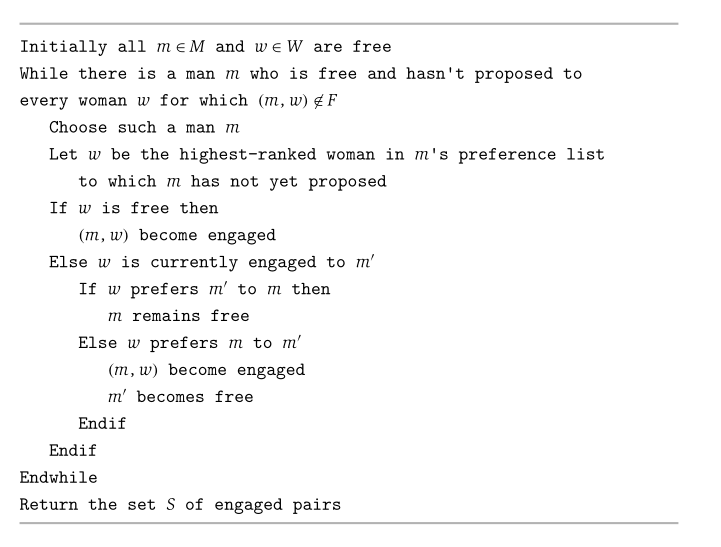
\includegraphics[scale=0.7]{Imagenes-Seccion1/cod1-1.PNG}

Ahora demostramos que esto produce un emparejamiento estable, bajo nuestra nueva definición de estabilidad.
Para empezar, los hechos $(1.1)$, $(1.2)$ y $(1.3)$ del texto permanecen verdaderos (en particular, el algoritmo terminará en un máximo de $n^{2}$ iteraciones). Además, no tenemos que preocuparnos por establecer que la coincidencia resultante $S$ es perfecta (de hecho, puede no serlo). También notamos un par de hechos adicionales. Si $m$ es un hombre que no es parte de un par en $S$, entonces $m$ debe haberle propuesto a cada mujer no prohibida; y si $w$ es una mujer que no es parte de un par en $S$, entonces debe ser que ningún hombre haya propuesto nunca $w$. Finalmente, solo necesitamos mostrar\\

(1.9) No hay inestabilidad con respecto a la $S$ igualada devuelta\\

Prueba. Nuestra definición general de inestabilidad tiene cuatro partes: Esto significa que debemos asegurarnos de que ninguna de las cuatro cosas malas ocurra.\\

Primero, supongamos que hay una inestabilidad de tipo (i), que consiste en pares $(m,w)$ y $(m',w')$ en S con la propiedad de que $(m,w')∉F$, m prefiere $w'$ a $w$, y $w'$ prefiere $m$ a $m'$. Se sigue que m debe haber propuesto a $w'$; así que rechacé a $m$, y por lo tanto ella prefiere que su compañero final sea una contradicción.\\

Luego, supongamos que hay una inestabilidad de tipo (ii), que consiste en un par $(m,w) \in S$, y un hombre $m'$, de modo que $m'$ no es parte de ningún par en el emparejamiento, $(m',w)∉F$, y $w$ prefiere $m'$ a $m$. Entonces $m'$ debe haber propuesto $w$ y haber sido rechazado; De nuevo, se sigue que $w$ prefiere a su compañero final como $m'$ -una contradicción.\\

En tercer lugar, supongamos que hay una inestabilidad de tipo (iii), que consiste en un par $(m,w) \in S$, y una mujer $w'$, por lo que $w'$ no es parte de ningún par en el emparejamiento, $(m,w')∉F$, y $m$ prefiere $w'$ a $w$. Entonces, ningún hombre se propuso a nada; en particular, $m$ nunca propuso $w'$, por lo que debe preferir $w$ a $w'$, una contradicción.\\

Finalmente, supongamos que hay una inestabilidad de tipo (iv), que consiste en un hombre $m$ y una mujer $w$, ninguno de los cuales es parte de ningún par en el emparejamiento, de modo que $(m,w)∉F$. Pero para que yo sea soltero, él debe haber propuesto a cada mujer no prohibida; en particular, debe haberlo propuesto, lo que significa que ya no estaría soltera, una contradicción. $ \blacksquare $\\


\newpage

\section{Análisis de algoritmos básicos}

\subsection{Trazabilidad computacional}

Un enfoque principal de este libro es encontrar algoritmos eficientes para problemás computacionales. En este nivel de generalidad, nuestro tema parece abarcar todo acerca de la ciencia de la computación; entonces, ¿cuál es nuestro enfoque específico aquí?. \\

Primero, trataremos de identificar los temás generales y los principios de diseño en el desarrollo de algoritmos. Buscaremos problemás paradigmáticos y enfoques que ilustran, con un mínimo de detalles irrelevantes, la aplicación básica de enfoques para diseñar algoritmos eficientes. Al mismo tiempo, sería inútil seguir estos principios de diseño en el vacío, entonces los problemás y enfoques que consideramos se derivan de cuestiones fundamentales que surgen fuera de la informática, y un estudio general de algoritmos resulta servir como una buena encuesta de ideas computacionales que surgen en muchas áreas. \\

Otra propiedad compartida por muchos de los problemás que estudiamos es su naturaleza fundamentalmente discreta. Es decir, al igual que el problema de apareamiento estable, implicará una búsqueda implícita sobre un gran conjunto de posibilidades combinatorias; y el objetivo será encontrar de manera eficiente una solución que satisfaga ciertas condiciones. \\

A medida que buscamos entender la noción general de eficiencia computacional, nos enfocaremos principalmente en la eficiencia en el tiempo de ejecución: queremos algoritmos que corran rápidamente. Pero es importante que los algoritmos sean eficientes en el uso de otros recursos también. En particular, la cantidad de espacio (o memoria) utilizada por un algoritmo es un problema que también surgirá en una serie de puntos en el libro, y veremos técnicas para reducir la cantidad de espacio necesario para realizar un cálculo.\\

\subsubsection*{Algunos intentos iniciales para definir la eficiencia}

La primera pregunta importante que debemos responder es la siguiente: ¿cómo deberíamos convertir la noción borrosa de un algoritmo "eficiente" en algo más concreto? 
Un primer intento de una definición de eficiencia es la siguiente. \\

\begin{center}\textit{Definición de eficiencia propuesta (1): un algoritmo es eficiente si, cuando es implementado, se ejecuta rápidamente en instancias de entrada reales.}\end{center}


 Dediquemos un poco de tiempo teniendo en cuenta esta definición. En cierto nivel, es difícil discutir: uno de los objetivos en la base de nuestro estudio de algoritmos es resolver problemás reales rápidamente. Y de hecho, hay un área importante de investigación dedicado a la implementación cuidadosa y el perfil de diferentes algoritmos para problemás discretos de computación.\\

 Pero hay algunas cosas cruciales que faltan en esta definición, incluso si nuestro objetivo principal es resolver instancias de problemás reales rápidamente en computadoras reales. Lo primero está la omisión de dónde, y qué tan bien implementamos un algoritmo.  Incluso los algoritmos malos pueden ejecutarse rápidamente cuando se aplican a pequeños casos de prueba en procesadores extremadamente  rápidos; incluso los buenos algoritmos pueden ejecutarse lentamente cuando están descuidadamente codificados. Además, ¿qué es una instancia de entrada "real"? No conocemos la gama completa de instancias de entrada que se encontrarán en la práctica, y algunas instancias de entradas pueden ser mucho más difíciles que otras. Finalmente, esta definición propuesta arriba no considera qué tan bien o mal puede ser un algoritmo a medida que crecen los tamaños de los problemás a niveles inesperados.\\
 
Una situación común es que dos algoritmos muy diferentes funcionen de manera comparable en las entradas de tamaño 100; multiplicamos el tamaño de la entrada por diez, y uno seguirá funcionando rápidamente mientras que el otro consume una gran cantidad de tiempo.  Entonces, lo que podríamos pedir es una definición concreta de eficiencia que sea independiente de la plataforma, independiente de la instancia y de valor predictivo con respecto al aumento de los tamaños de entrada. 
Antes de enfocarnos en cualquier consecuencia específica de esta afirmación, al menos podemos explorar su sugerencia implícita de alto nivel: necesitamos tomar una visión más matemática de la situación.\\

 Podemos usar el problema de emparejamiento estable como un ejemplo para guiarnos. La entrada tiene un parámetro de "tamaño" natural $N$; podríamos tomar esto como el tamaño total de la representación de todas las listas de preferencias, ya que esto es lo que cualquier algoritmo recibirá para el problema como entrada. $N$ está estrechamente relacionado con el otro parámetro natural en este problema: $n$, el número de hombres y el número de mujeres. Ya que son $2n$ listas de preferencia, cada una de longitud $n$, podemos ver $N = 2n^2$, suprimiendo detalles de cómo se representan los datos. 
Al considerar el problema, buscaremos describir un algoritmo en un nivel alto, y luego analizar su tiempo de ejecución matemáticamente como una función de este tamaño de entrada $N$. \\

\subsubsection*{Tiempos de ejecución de peores casos y búsqueda por fuerza bruta} 

Para empezar, nos enfocaremos en analizar el peor tiempo de ejecución: lo haremos buscando un límite en el mayor tiempo de ejecución posible que el algoritmo podría tener sobre todas las entradas de un tamaño dado $N$, y ver cómo esto crece con $N$. \\

El enfoque en el peor de los casos parece inicialmente bastante draconiano: ¿y si un algoritmo funciona bien en la mayoría de los casos y solo tiene algunas entradas patológicas en que es muy lento? Esto ciertamente es un problema en algunos casos, pero en general se ha encontrado que el peor análisis de un algoritmo hace un trabajo razonable de capturar su eficiencia en la práctica. \\

Por otra parte, una vez que hemos decidido ir la ruta del análisis matemático, es difícil encontrar una alternativa efectiva a peor caso de análisis. 
Análisis de casos promedio: la alternativa más atractiva, en el que se estudia el rendimiento de un algoritmo promediado sobre instancias "aleatorias", a veces puede proporcionar información considerable, pero muy a menudo puede también convertirse en un atolladero. \\

Como hemos observado anteriormente, es muy difícil expresar la gama completa de instancias de entrada que surgen en la práctica, y así intentar estudiar el rendimiento del algoritmo en instancias de entrada "aleatorias" puede convertirse rápidamente en debates sobre cómo se debe generar una entrada aleatoria: el mismo algoritmo puede funcionar muy bien en una clase de entradas aleatorias y muy mal en otra. Después de todo, las entradas reales a un algoritmo generalmente no se están produciendo de una distribución aleatoria, por lo que el análisis de caso promedio nos arriesga a decirnos más sobre los medios por los cuales se generaron las entradas aleatorias que sobre el algoritmo en sí. \\

Entonces, en general, pensaremos sobre el peor caso de tiempo de ejecución en el análisis de un algoritmo. Pero, ¿cual es el punto de referencia analítico razonable que nos puede decir si un límite de tiempo de ejecución es impresionante o débil? Una primera guía simple es en comparación con la búsqueda de fuerza bruta en el espacio de búsqueda de posibles soluciones. \\

Volvamos al ejemplo del problema de emparejamiento estable. Incluso cuando el tamaño de una instancia de entrada de emparejamiento estable es relativamente pequeño, la búsqueda el espacio que define es enorme (hay $n!$ posibles combinaciones perfectas entre $n$ hombres y $n$ mujeres), y necesitamos encontrar una pareja que sea estable. el algoritmo natural de "fuerza bruta" para este problema atravesaría todo perfecto emparejamientos por enumeración, comprobando cada uno para ver si es estable. Lo sorprendente, en cierto sentido, para nuestra solución del problema de apareamiento estable es que es necesario pasar tiempo proporcional solo a $N$ para encontrar una coincidencia estable de entre este espacio de posibilidades estupendamente grande. Esta fue una conclusión que alcanzamos en un nivel analítico. No implementamos el algoritmo y lo intentamos en listas de preferencia de muestra; razonamos al respecto matemáticamente. Sin embargo, al mismo tiempo, nuestro análisis indicó cómo el algoritmo podría implementarse en práctica y dio evidencia bastante concluyente de que sería una gran mejora sobre una enumeración exhaustiva. \\

Este será un tema común en la mayoría de los problemás que estudiamos: una representación compacta, especificando implícitamente un espacio de búsqueda gigante. Para la mayoría de estos problemás, habrá una solución obvia de fuerza bruta: probar todas las posibilidades y ver si alguna de ellas funciona. No solo este enfoque casi siempre es demásiado lento para ser útil, sino también es un colapso intelectual; no proporciona absolutamente ninguna idea de la estructura del problema que estamos estudiando. Y entonces si hay un hilo común en los algoritmos que enfatizamos en este libro, sería la siguiente definición alternativa de eficiencia. \\

\begin{center}\textit{Definición de eficiencia propuesta (2): un algoritmo es eficiente si se logra cualitativamente mejor rendimiento del peor caso, en un nivel analítico, que la búsqueda por fuerza bruta.}\end{center}

Esta será una definición de trabajo muy útil para nosotros. Algoritmos que mejoran sustancialmente la búsqueda de fuerza bruta casi siempre contienen una valiosa idea heurística que los hace funcionar; y ellos nos dicen algo acerca de la estructura intrínseca y la capacidad de procesamiento computacional del problema subyacente  en si mismo.\\

 Pero si hay un problema con nuestra segunda definición de trabajo, es algo vaga. ¿Qué queremos decir con "rendimiento cualitativamente mejor"? Esto sugiere que consideramos el tiempo de ejecución real de los algoritmos con más cuidado, y probemos para cuantificar lo que sería un tiempo de ejecución razonable. \\

\subsubsection*{Tiempo polinomial como definición de eficiencia} 

Cuando las personas comenzaron a analizar algoritmos matemáticamente discretos, un hilo de investigación que comenzó a cobrar impulso durante la década de 1960, fue cómo cuantificar la noción de un "razonable" tiempo de ejecución. Los espacios de búsqueda de problemás combinatorios naturales tienden a crecer exponencialmente en el tamaño $N$ de la entrada; si el tamaño de entrada aumenta en uno, el número de posibilidades aumenta multiplicativamente. Queremos un buen algoritmo para que ese problema tenga una mejor propiedad de escala: cuando el tamaño de entrada aumenta en un factor constante, es decir, un factor de 2, el algoritmo debería reducir la velocidad por un factor constante $C$. \\

Aritméticamente, podemos formular este comportamiento de escala de la siguiente manera. Supongamos que un algoritmo tiene la siguiente propiedad: hay constantes absolutas $c>0$ y $d>0$ tales que en cada instancia de entrada de tamaño $N$, su tiempo de ejecución está limitado por $cN^d$ pasos computacionales primitivos. (En otras palabras,  el tiempo de ejecución es como máximo proporcional a $N^d$.) Por ahora, nos mantendremos deliberadamente vagos en lo que queremos decir con la noción de un "paso computacional primitivo" - pero se puede formalizar fácilmente en un modelo donde cada paso corresponde a una sola instrucción en lenguaje ensamblador en un procesador estándar, o una línea de un lenguaje de programación estándar como C o Java-. En cualquier caso, si el tiempo de ejecución es limitado, por algunos $c$ y $d$, entonces decimos que el algoritmo tiene un tiempo de ejecución polinomial, o que es un algoritmo de tiempo polinomial. Notemos que cualquier límite de tiempo polinomial tiene la propiedad de escala que estamos buscando. Si el tamaño de entrada aumenta de $N$ a $2N$, aumenta el límite en el tiempo de ejecución de $cN^d$ a $c(2N)^d = c2^dN^d$, que es una disminución en un factor de $2^d$. Como $d$ es una constante, entonces lo es $2^d$; por supuesto, como uno podría esperar, polinomios de menor grado exhiben un mejor comportamiento de escalamiento que los polinomios de alto grado. A partir de esta noción, y la intuición expresada anteriormente, emerge nuestro tercer intento de una definición de eficiencia. \\

\begin{center}\textit{Definición de eficiencia propuesta (3): un algoritmo es eficiente si tiene un tiempo de ejecución polinómica.}\end{center}    
    
Nuestra segunda definición parecía demásiado vaga pero esta parece mucho más descriptiva. ¿Existirá un algoritmo con tiempo de ejecución proporcional a $n^{100}$ - y, por lo tanto, polinómico - irremediablemente ineficiente? ¿Estaríamos relativamente satisfechos con un tiempo de ejecución no polinomial de $n^{1+.02(log n)}$ ? Las respuestas son, por supuesto, "sí" y "sí". Y, de hecho, por mucho que uno pueda tratar de motivar de manera abstracta la definición de eficiencia en términos de tiempo polinomial, una justificación primaria para esto es: realmente funciona. Problemás para los cuales existen algoritmos de tiempo polinomial casi invariablemente resultan tener algoritmos con tiempos de funcionamiento proporcionales a polinomios de crecimiento muy moderados como $n$, $nlog n$, $n^2$ o $n^3$. Por el contrario, en problemás para los cuales no hay tiempo polinomial se sabe que el algoritmo es muy difícil en la práctica. Ciertamente hay excepciones a este principio en ambas direcciones: hay casos, por ejemplo, en que un algoritmo con el peor comportamiento exponencial generalmente funciona bien sobre los tipos de instancias que surgen en la práctica; y también hay casos donde el mejor algoritmo de tiempo polinomial para un problema es completamente impracticable debido a grandes constantes o un alto exponente en el polinomio. Todo esto sirve para reforzar el punto de que nuestro énfasis, en el peor de los casos, acerca del tiempo polinomial límite es solo una abstracción de situaciones prácticas. Pero abrumadoramente, la definición matemática concreta de tiempo polinomial ha resultado correlativamente sorprendentemente en la práctica a lo que observamos sobre la eficiencia de algoritmos y la capacidad de tratar problemás en la vida real.\\

Una razón más por la cual el formalismo matemático y la evidencia empírica parecen alinearse bien en el caso de la solvencia de tiempo polinomial es que la diferencia  entre las tasas de crecimiento de funciones polinomiales y exponenciales son enorme.
Supongamos, por ejemplo, que tenemos un procesador que ejecuta un millón de instrucciones de alto nivel por segundo, y tenemos algoritmos con límites de tiempo de ejecución de $n$, $nlog(2n)$, $n^2$, $n^3$, $1.5^n$, $2^n$, y $n!$. En la figura \ref{Tabla 2.1}, mostramos los tiempos de ejecución de estos algoritmos (en segundos, minutos, días, o años) para entradas de tamaño n = 10, 30, 50, 100, 1,000, 10,000, 100,000 y 1,000,000. Hay un beneficio final fundamental para hacer nuestra definición de eficiencia tan específico: se vuelve negable. Se hace posible expresar la noción que no existe un algoritmo eficiente para un problema en particular. En cierto sentido, ser capaz de hacer esto es un requisito previo para convertir nuestro estudio de algoritmos en una buena ciencia, porque nos permite preguntar sobre la existencia o inexistencia de algoritmos eficientes como una pregunta bien definida. Por el contrario, las definiciones anteriores eran completamente subjetivas y, por lo tanto, limitaban la medida en que podíamos discutir ciertos asuntos en términos concretos. \\

\begin{figure}[h] 
  \centering
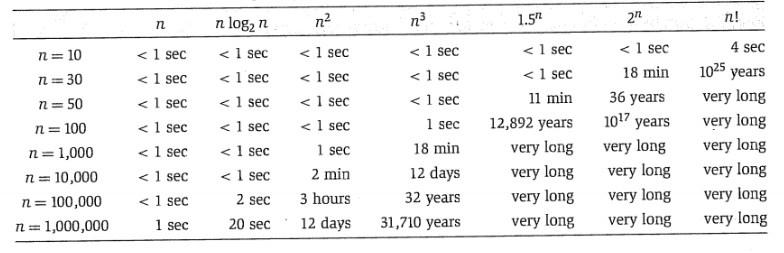
\includegraphics[width=1\textwidth]{Imagenes-Seccion1/Figura1.PNG}
  \caption{Tabla 2.1}
  \label{Tabla 2.1}
\end{figure}

En particular, la primera de nuestras definiciones, que estaba ligada a la implementación específica de un algoritmo, convirtió la eficiencia en un objetivo en movimiento: a medida que las velocidades del procesador aumentan, cada vez más algoritmos entran dentro de esta noción de eficiencia. Nuestra definición en términos de tiempo polinomial es mucho más una noción absoluta; está estrechamente relacionado con la idea de que cada problema tiene un nivel intrínseco de capacidad de procesamiento computacional: algunos admiten soluciones eficientes y otros no.\\

 \subsection{Orden de crecimiento asintótico}

Nuestra discusión sobre la capacidad de computación, ha resultado  estar basado en nuestra capacidad de expresar la noción de que el tiempo de ejecución, en el peor caso, de un algoritmo con $n$ entradas de datos crece a un ritmo que es proporcional a alguna función $f(n)$. La función $f(n)$ se convierte en un límite en el tiempo de ejecución del algoritmo. Ahora discutimos un marco para hablar sobre este concepto. \\

Expresaremos principalmente algoritmos en el estilo de pseudo-código que utilizamos para el algoritmo de Gale-Shapley. A veces necesitaremos ser más formales, pero este estilo de algoritmos específicos será completamente adecuado para la mayoría de los propósitos. Cuando proporcionamos un límite en el tiempo de ejecución de un algoritmo, generalmente contaremos el número de pasos de pseudo-código que son ejecutados; en este contexto, un paso consistirá en asignar un valor a un variable, buscar una entrada en una matriz, seguir un puntero o realizar una operación aritmética en un entero de tamaño fijo.\\

Cuando buscamos decir algo sobre el tiempo de ejecución de un algoritmo en entradas de tamaño $n$, una cosa a la que podríamos apuntar sería a una declaración muy concreta como: "En cualquier entrada de tamaño $n$, el algoritmo se ejecuta a lo sumo a $1.62n^2 + 3.5n + 8$ pasos." Esta puede ser una declaración interesante en algunos contextos, pero como un objetivo general, hay varias cosas mal con eso. Primero, obtener una precisión puede ser una actividad agotadora, y más detallada de lo que queríamos de todos modos. Segundo, como nuestro objetivo final es identificar amplias clases de algoritmos que tengan un comportamiento similar, en realidad nos gustaría clasificar los tiempos de ejecución en una versión más general para que las similitudes entre los diferentes algoritmos, y diferentes problemás, aparezcan con mayor claridad. Y finalmente, detallar extremadamente las declaraciones sobre el número de pasos que ejecuta un algoritmo son a menudo -en un sentido fuerte- sin sentido. Como acabamos de comentar, generalmente contaremos pasos en una especificación de pseudo-código de un algoritmo que se asemeja a un lenguaje de alto nivel de programación. Cada uno de estos pasos generalmente se desarrollará en un número fijo de pasos primitivos cuando el programa se compila en una representación intermedia, y luego en algunos otros pasos dependiendo de la arquitectura particular que se use para hacer la computación. Así que lo máximo que podemos decir con seguridad es que, a medida que observamos los diferentes niveles de abstracción computacional, la noción de un "paso" puede crecer o reducirse por un factor constante. Por ejemplo, si se necesitan 25 instrucciones de máquina de bajo nivel para realizar una operación en nuestro lenguaje de alto nivel, luego nuestro algoritmo que tomó como máximo $1.62n^2 + 3.5n + 8$ pasos, también se puede ejecutar tomando $40.5n^2 + 87.5n + 200$ pasos cuando lo analizamos a un nivel más cercano al hardware real.\\

\subsubsection*{$O$ $\Omega $ y $\Theta$}

Por todas estas razones, queremos expresar la tasa de crecimiento de los tiempos de ejecución y otras funciones de una manera que es insensible a factores constantes y de bajo orden de términos. En otras palabras, nos gustaría poder tomar un tiempo de ejecución como el que discutimos anteriormente, $1.62n^2 + 3.5n + 8$, y decir que crece como $n^2$, hasta factores constantes. Ahora discutimos una forma precisa de hacer esto.\\


\subsubsection*{Límites superiores asintóticos.}

Sea $T(n)$ sea una función, digamos, el peor de los casos de tiempo de un determinado algoritmo en una entrada de tamaño $n$. (Asumiremos que todas las funciones de las que hablamos aquí toman valores no negativos.) Dada otra función $f(n)$, decimos que $T(n)$ es $O(f(n))$ (leída como $"T (n)$ es orden $f(n)"$) si, para $n$ suficientemente grande, la función $T(n)$ está acotada superiormente por un múltiplo constante de $f(n)$. También a veces escribiremos esto como $T (n) = O(f(n))$. Más precisamente, $T(n)$ es $O(f(n))$ si existen constantes $c > 0$ y $n_0 ≥ 0$, de modo que para todo $n ≥ n_0$, tenemos $T(n) ≤ c f (n)$. En este caso, diremos que $T$ es  acotada superiormente por $f$. Es importante tener en cuenta que esta definición requiere que exista una $c$ constante que funcione para todos n; en particular, $c$ no puede depender de $n$. \\

Veamos un ejemplo de cómo esta definición nos permite expresar límites superiores en tiempos de ejecución. Consideremos un algoritmo cuyo tiempo de ejecución (como en la anterior discusión) tiene la forma $T (n) = pn^2 + qn + r$ para las constantes positivas $p$, $q$, y $r$. Nos gustaría afirmar que cualquier función de este tipo es $O(n^2)$. Para ver por qué, notamos que para todo $n ≥ 1$, tenemos $qn ≤ qn^2$ y $r ≤ rn^2$. Entonces podemos escribir: 

\begin{center}$T (n) = pn^2 + qn + r  ≤ pn^2+ qn^2 + rn^2 = (p + q + r)n^2$ para todo $n ≥ 1$\end{center}

Esta desigualdad es exactamente lo que la definición de orden $O(.)$ requiere: $T(n) ≤ cn^2$, donde $c = p + q + r$. \\

Tengamos en cuenta que $O(.)$ expresa solo un límite superior, no la tasa de crecimiento exacta de la función. Por ejemplo, al igual que afirmamos que la función $T (n) = pn^2 + qn + r$ es $O(n^2)$, también es correcto decir que es $O(n^3)$. De hecho, solo argumentamos que $T (n) ≤ (p + q + r) n^2$, y dado que también tenemos $n^2 ≤ n^3$, podemos concluir que $T (n) ≤ (p + q + r) n^3$ como la definición de $O(n^3)$ requiere. El hecho de que una función puede tener muchos límites superiores no es solo un truco del notación; aparece en el análisis de los tiempos de ejecución también. Hay casos donde se ha demostrado que un algoritmo tiene tiempo de ejecución $O(n^3)$; algunos años pasan, las personas analizan el mismo algoritmo con más cuidado, y muestran que de hecho, su tiempo de ejecución es $O (n^2)$. No hubo nada malo con el primer resultado; era un límite superior correcto. Simplemente que no era el "más estricto" posible tiempo de ejecución. \\



\subsubsection*{Límites inferiores asintóticos}

Hay una notación complementaria para el nivel inferior de límites. A menudo, cuando analizamos un algoritmo, digamos que hemos demostrado que su peor tiempo de ejecución $T (n)$ es $O (n^2) $ entonces queremos mostrar que esta acotación superior es la mejor posible. Para hacer esto, queremos expresar la noción de que para  $n$ arbitrariamente grandes, la función $T(n)$ es al menos un múltiplo constante de alguna función específica $f(n)$. (En este ejemplo, $f(n)$ pasa a ser $n^2$). Por lo tanto, decir que $T(n)$ es $\Omega(f (n))$ (también escrito $ T (n) = (f (n)))$ equivale a decir que existen constantes $e > 0$ y $n_0 ≥ 0$, de modo que para todo $n ≥ n_0$, tenemos $T (n) ≥ eF(n)$. Por analogía con la notación  $O(.)$, nos referiremos a $T$ en este caso como acotada anteriormente por $f$. De nuevo, tengamos en cuenta que la constante $e$ debe ser fija, independiente de $n$. \\

Esta definición funciona igual que $O(.)$, excepto que estamos limitando la función $T(n)$ desde abajo, en lugar que desde arriba. Por ejemplo, regresemos a la función $T (n) = pn^2+ qn + r$,  donde $p$, $q$, y $r$ son constantes positivas, supongamos que $T (n)= \Omega(n^2)$. Considerando que establecimos la cota superior "inflando" los términos en $ T(n)$ hasta que aparezca una constante de $n^2$, ahora necesitamos hacer lo contrario: necesitamos reducir el tamaño de $T(n)$ hasta que se vea como un tiempo constante $n^2$. No es difícil hacer esto; para todos $n ≥ 0$, tenemos $T (n) = pn^2 + qn + r ≥ pn^2$, que cumple con lo requerido por la definición de $\Omega(.)$ con $e = p> 0$. Así como discutimos la noción de límites superiores "más estrictos" y "más débiles", el mismo problema surge para los límites inferiores. Por ejemplo, es correcto decir que nuestra función $T (n) = pn^2 + qn + r$ es $\Omega(n)$, ya que $T (n) ≥ pn^2 ≥ pn$.\\

\subsubsection*{Límites asintóticamente estrechos}

Si podemos demostrar que un tiempo de ejecución $T(n)$ es $O(f(n))$ y también $\Omega(f(n))$, entonces, en un sentido natural, hemos encontrado la acotación "correcta": $T(n)$ crece exactamente como $f(n)$ dentro de un factor constante. Esto por ejemplo, es la conclusión que podemos extraer del hecho de que $T(n) = pn^2 + q^n + r$ es tanto $O(n^2)$ como $\Omega(n^2)$. \\

Hay una notación para expresar esto: si una función $T(n)$ es tanto $O(f(n))$ como $\Omega(f (n))$, decimos que $T(n)$ es $\Theta (f (n))$. En este caso, decimos que $f(n)$ es un asintóticamente ajustado por $T(n)$. Entonces, por ejemplo, nuestro análisis anterior muestra que $T (n) = pn^2 + q^n + r$ es $\Theta(n^2)$.\\

Los límites asintóticamente estrechos en los peores casos de tiempos de ejecución son buenos para encontrar, ya que caracterizan el peor de los casos de un algoritmo hasta factores constantes. Y como muestra la definición de $\Theta(.)$ podemos obtener dichos límites al cerrar la brecha entre un límite superior y un límite inferior ligado. Por ejemplo, a veces leeremos una oración (redactada de manera ligeramente informal) como "Se ha mostrado una cota superior de $O(n^3)$ en el peor de los casos de tiempo de ejecución del algoritmo, pero no se conoce ningún ejemplo en el que algoritmo se ejecuta para más de $\Omega(n^2)$ pasos."  A veces, también se puede obtener un límite asintóticamente estrecho directamente hallando un límite cuando $n$ va al infinito. Esencialmente, si el cociente de las funciones $f(n)$ y $g(n)$ convergen a una constante positiva cuando $n$ va al infinito, entonces $f(n) = \Theta(g(n))$.  \\
\\
(2.1) Sean f y g 2 funciones tales que
\begin{equation}
\displaystyle\lim_{n \to \infty} \frac{f(n)}{g(n)}
\end{equation}
existe y es igual a algún numero $c > 0$. Entonces $f(n) =  \Theta(g(n))$\\

\textbf{Demostración}. Usamos el hecho de que el limite existe y es positivo para mostrar que $f(n) = O(g(n))$ y $f(n) = \Omega(g(n))$, como lo requiere la definicion de $\Theta(.)$\\

Del hecho de que
\begin{equation}
\displaystyle\lim_{n \to \infty} \frac{f(n)}{g(n)} = c > 0
\end{equation}
Se sigue de la definición de limite que existe algun $n_0$ a partir del cual la relación esta entre $\frac{1}{2}c$ y $2c$ $.:.$ $f(n) \leq 2c g(n)$ para todo $n \geq n_0$, lo que implica que $f(n) = O(g(n))$; y $f(n) \geq \frac{1}{2}c g(n)$ para todo $n \geq n_0$, lo que implica que $f(n) = \Omega(g(n))$. $\blacksquare$.\\

\subsubsection*{Propiedades de las tasas de crecimiento asintótico (revisar)}

Habiendo visto las definiciones de O,, y, es útil explorar algunas de sus propiedades básicas.

\textbf{Transitividad}. Una primera propiedad es la transitividad: si una función f es superior de manera asintótica por una función g, y si g, a su vez, es asintóticamente superior por una función h, entonces f es asintóticamente límite superior por h. Una propiedad similar se mantiene para los límites inferiores. Escribimos esto de manera más precisa de la siguiente manera.\\

(a) If \(f=O(g)\) and \(g=O(h)\), then \(f=O(h)\).\\

(b) If \(f=\Omega(g)\) and \(g=\Omega(h)\), then \(f=\Omega(h)\).\\
 
\textbf{Demostración}.  Vamos a probar la parte (a) de este reclamo; la prueba de la parte (b) es muy similar. Para (a), se nos da que para algunas constantes $c'$ y $n_0'$, tenemos $f(n)≤cg(n)$ para todo $n≥n_0$. Además, para algunas constantes (potencialmente diferentes) $c'$ y $n_0'$, tenemos $g(n)≤c'h(n)$ para todo $n ≥ n_0'$. Por lo tanto, considere cualquier número n que sea al menos tan grande como $n_0$ y $n_0'$. Tenemos $f(n)≤cg(n) ≤ cc'h(n)$, y así $f(n)≤cc'h(n)$ para todo $n≥max(n0, n_0')$. Esta última desigualdad es exactamente lo que se requiere para mostrar que $f=O(h)$. $\blacksquare$ \\

Combinando las partes (a) y (b) de (2.2), podemos obtener un resultado similar para los límites estrechos asintóticamente. Supongamos que sabemos que $f=\Theta(g)$ y que $g=\Theta(h)$. Entonces, dado que $f=O(g)$ y $g=O(h)$, sabemos por la parte (a) que $f=O(h)$; dado que $f=\Omega(g)$ y $g=\Omega(h)$, sabemos por la parte (b) que $f=\Omega(h)$. Se deduce que $f=\Theta(h)$. Por lo tanto, hemos demostrado.\\

(2.3) Si $f=\Theta(g)$ y $g=\Theta(h)$, entonces $f=\Theta(h)$\\

\textbf{Sumás de funciones}. También es útil tener resultados que cuantifiquen el efecto de agregar dos funciones. Primero, si tenemos un límite superior asintótico que se aplica a cada una de las dos funciones $f$ y $g$, entonces se aplica a su suma.\\

(2.4) Supongamos que $f$ y $g$ son dos funciones tales que para alguna otra función $h$, tenemos $f = O (h)$ y $g = O (h)$. Entonces $f + g = O (h)$.\\

\textbf{Demostración}. Se nos da que para algunas constantes $c$ y $n_0$, tenemos $f(n)≤ch(n)$ para todo $n≥n_0$. Además, para algunas constantes (potencialmente diferentes) $c'$ y $n_0'$, tenemos $g(n)≤c'h(n)$ para todo $n≥n_0'$. Por lo tanto, considere cualquier número $n$ que sea al menos tan grande como $n_0$ y $n_0'$. Tenemos $f(n) + g (n) ≤ ch (n) + c'h (n)$. Así $f (n) + g (n) ≤ (c' + c) h (n)$ para todo $n≥max(n0, n_0')$, que es exactamente lo que se requiere para mostrar que $f + g = O (h)$.$\blacksquare$ \\

Hay una generalización de esto en sumás de un número constante fijo de funciones $k$, donde $k$ puede ser mayor que dos. El resultado se puede expresar de la siguiente manera; omitimos la prueba, ya que es esencialmente la misma que la prueba de (2.4), adaptada a sumás consistentes en $k$ términos en lugar de solo dos.\\

(2.5) Sea $k$ una constante fija, y que $f_1, f_2, ..., f_k$ y $h$ sean funciones tales que $f_i = O(h)$ para todo $i$. Luego $f_1 + f_2 + ... + f_k = O (h)$\\

También hay una consecuencia de (2.4) que cubre el siguiente tipo de situación. Con frecuencia sucede que estamos analizando un algoritmo con dos partes de alto nivel, y es fácil mostrar que una de las dos partes es más lenta que la otra. Nos gustaría poder decir que el tiempo de ejecución de todo el algoritmo es asintóticamente comparable con el tiempo de ejecución de la parte lenta. Dado que el tiempo total de ejecución es una suma de dos funciones (los tiempos de ejecución de las dos partes), los resultados en límites asintóticos para sumás de funciones son directamente relevantes.\\


(2.6) Supongamos que $f$ y $g$ son dos funciones (toman valores no negativos) tales que $g = O (f)$. Entonces $f + g = \Theta(f)$. En otras palabras, $f$ es un límite asintóticamente ajustado para la función combinada $f + g$.\\

\textbf{Demostración}. Claramente, $f + g = \Theta (f)$, ya que para todo $n ≥ 0$, tenemos $f (n) + g (n) ≥ f (n)$. Entonces, para completar la prueba, necesitamos mostrar que $f + g = O (f)$. \\

Pero esta es una consecuencia directa de (2.4): se nos da el hecho de que $g = O (f)$, y también $f = O (f)$ se cumple para cualquier función, entonces por (2.4) tenemos $f + g = O (f)$. $\blacksquare$ \\

Este resultado también se extiende a la suma de cualquier cantidad fija y constante de funciones: la más rápida de todas las funciones es un límite asintóticamente estrecho para la suma\\

\subsubsection*{Límites asintóticos para algunas funciones comunes (revisar)}

Hay una serie de funciones que surgen repetidamente en el análisis de algoritmos, y es útil considerar las propiedades asintóticas de algunos de los más básicos: polinomios, logaritmos y exponenciales.\\

\textbf{Polinomial}. Recuerde que un polinomio es una función que puede escribirse con la forma $f(n) = a_0 + a_1n + a_2n^2 + ... + a_dn^d$ para una constante entera $d> 0$, donde el coeficiente final $a_d$ es no cero. Este valor $d$ se llama el grado del polinomio. Por ejemplo, las funciones de la forma $pn^2 + qn + r$ (con $p \neq 0$) que consideramos anteriormente son polinomios de grado $2$.\\

Un hecho básico sobre los polinomios es que su tasa de crecimiento asintótico está determinada por su "término de orden alto", el que determina el grado. Declaramos esto más formalmente en el siguiente reclamo. Como aquí nos ocupamos únicamente de las funciones que toman valores no negativos, restringiremos nuestra atención a los polinomios para los cuales el término de orden superior tiene un coeficiente positivo a $d>0$.\\

(2.7) Sea $f$ un polinomio de grado $d$, en el cual el coeficiente $a_d$ es positivo. Entonces $f = O (n^d)$.\\

\textbf{Demostración}. Escribimos $f = a_0 + a_1^n + a_2n^2 + ... + a_dn^d$, donde a $d>0$. El límite superior es una aplicación directa de (2.5). Primero, observe que los coeficientes a $j$ para $j<d$ pueden ser negativos, pero en cualquier caso tenemos $a_jn^j ≤ |a_j|n^d$ para todo $n≥1$. Por lo tanto, cada término en el polinomio es $O(n^d)$. Como $f$ es la suma de un número constante de funciones, cada una de las cuales es $O(n^d)$, se sigue de (2.5) que $f$ es $O(n^d)$. $\blacksquare$\\

También se puede demostrar que bajo las condiciones de (2.7), tenemos $f = \Omega(n ^ d)$, y por lo tanto se sigue que de hecho $f = \Theta(n^d)$.

Este es un buen punto para discutir la relación entre estos tipos de límites asintóticos y la noción de tiempo polinomial, al cual llegamos en la sección anterior como una manera de formalizar el concepto de eficiencia más elusivo. Usando la notación $O(·)$, es fácil definir formalmente el tiempo polinomial: un algoritmo de tiempo polinomial es aquel cuyo tiempo de ejecución $T(n)$ es $O(n^d)$ para alguna constante $d$, donde $d$ es independiente del tamaño de entrada.\\

Por lo tanto, los algoritmos con límites de tiempo de ejecución como $O(n^2)$ y $O(n^3)$ son algoritmos de tiempo polinomial. Pero es importante darse cuenta de que un algoritmo puede ser un tiempo polinomial, incluso si su tiempo de ejecución no se escribe como $n$ elevado a una potencia entera. Para empezar, varios algoritmos tienen tiempos de ejecución de la forma $O(n^x)$ para un número $x$ que no es un número entero. Por ejemplo, en el Capítulo 5 veremos un algoritmo cuyo tiempo de ejecución es $O(n^{1.59})$; también veremos exponentes menos de 1, como en límites como $O(√n) = O (n^{1/2})$\\

Para tomar otro tipo de ejemplo común, veremos muchos algoritmos cuyos tiempos de ejecución tienen la forma $O(nlogn)$. Tales algoritmos también son tiempo polinomial: como veremos a continuación, $log n ≤ n$ para todo $n ≥ 1$, y por lo tanto $n log n ≤ n^2$ para todo $n ≥ 1$. En otras palabras, si un algoritmo tiene tiempo de ejecución $O (n log n)$, entonces también tiene tiempo de ejecución $O (n^2)$, por lo que es un algoritmo de tiempo polinomial.\\

\textbf{Logarítmico}. Recuerde que $log_bn$ es el número $x$ tal que $b^x = n$. Una manera de tener una idea aproximada de cuán rápido crece $log_bn$ es observar que, si lo redondeamos al entero más cercano, es uno menos que el número de dígitos en la representación base-$b$ del número $n$. (Por lo tanto, por ejemplo, $1+ log_2 n$, redondeado hacia abajo, es el número de bits necesarios para representar $n$.).\\

Entonces, los logaritmos son funciones que crecen muy lentamente. En particular, para cada base $b$, la función $log_b n$ está limitada asintóticamente por cada función de la forma $n^x$, incluso para valores (no enteros) de $x$ arbitrario próximo a $0$.\\

(2.8) Por cada $b>1$ y cada $x>0$, tenemos $log_bn = O(n^x)$\\

Uno puede traducir directamente entre logaritmos de diferentes bases usando la siguiente identidad fundamental:\\

\begin{equation}
log_an = \frac{log_bn}{log_ba}
\end{equation}
Se sigue de la definición de limite que existe algun $n_0$ a partir del cual la relación esta entre $\frac{1}{2}c$ y $2c$.

Esta ecuación explica por qué a menudo notarás personas escribiendo límites como $O(log(n))$ sin indicar la base del logaritmo. Este no es un uso descuidado: la identidad anterior dice que $log_an = \frac{1}{log_ba}.log_bn$ entonces el punto es que $log_an = (log_bn)$, y la base del logaritmo no es importante cuando se escriben límites usando notación asintótica.\\

\textbf{Exponenciales} Las funciones exponenciales son funciones de la forma $f(n) = r^n$ para alguna base constante $r$. Aquí nos ocuparemos del caso en el que $r>1$, que da como resultado una función de crecimiento muy rápido.\\

En particular, cuando los polinomios se elevan a un exponente fijo, los exponenciales elevan un número fijo a $n$ como potencia; esto conduce a tasas de crecimiento mucho más rápidas. Una forma de resumir la relación entre polinomios y exponenciales es la siguiente.\\

(2.9) Por cada $r>1$ y cada $d>0$, tenemos $n^d=O(r^n)$.\\

En particular, cada exponencial crece más rápido que cualquier polinomio. Y como vimos en la Tabla 2.1, cuando se ingresan los valores reales de $n$, las diferencias en las tasas de crecimiento son realmente bastante impresionantes\\

Del mismo modo que las personas escriben $O(log n)$ sin especificar la base, también verán que las personas escriben "El tiempo de ejecución de este algoritmo es exponencial", sin especificar qué función exponencial tienen en mente. A diferencia del uso liberal de $log n$, que se justifica ignorando factores constantes, este uso genérico del término "exponencial" es algo descuidado. En particular, para diferentes bases $r>s>1$, nunca es el caso que $r^n = \Theta(s^n)$. De hecho, esto requeriría que para alguna constante $c>0$, tendríamos $r^n ≤ cs^n$ para todos los $n$ suficientemente grandes. Pero reorganizar esta desigualdad daría $(r/s)^n ≤ c$ para todos los $n$ suficientemente grandes $n$. Como $r>s$, la expresión $(r/s)^n$ tiende a infinito con $n$, y por lo tanto no puede permanecer limitada por una constante fija $c$.\\

Así que hablando de manera asintótica, las funciones exponenciales son todas diferentes. Aún así, generalmente está claro lo que las personas quieren decir cuando escriben inexactamente: "El tiempo de ejecución de este algoritmo es exponencial": típicamente significan que el tiempo de ejecución crece al menos tan rápido como una función exponencial, y todas las exponenciales crecen tan rápido que podemos descarte este algoritmo sin resolver más detalles del tiempo exacto de ejecución. Esto no es del todo justo. Ocasionalmente, hay más en juego con un algoritmo exponencial que el primero que aparece, como veremos, por ejemplo, en el Capítulo 10; pero como argumentamos en la primera sección de este capítulo, es una regla general razonable.\\

Tomados en conjunto, entonces, los logaritmos, polinomios y exponenciales sirven como puntos de referencia útiles en el rango de posibles funciones que se encuentran al analizar los tiempos de ejecución. Los logaritmos crecen más lentamente que los polinomios, y los polinomios crecen más lentamente que los exponenciales.\\

\subsection{Implementando el algoritmo de emparejamiento estable usando listas y arreglos}

Hemos visto un enfoque general para expresar límites en el tiempo de ejecución de un algoritmo. Para analizar de forma asintótica el tiempo de ejecución de un algoritmo expresado en una manera de alto nivel, como expresamos el algoritmo de emparejamiento estable de Gale Shapley en el Capítulo 1, por ejemplo, no es necesario programar, compilar y ejecutar, pero hay que pensar en cómo se representarán y manipularán los datos en una implementación del algoritmo, de modo que se vincule el número de pasos computacionales necesarios..\\

La implementación de algoritmos básicos que usan estructuras de datos es algo con lo que probablemente haya tenido alguna experiencia. En este libro, las estructuras de datos se tratarán en el contexto de la implementación de algoritmos específicos, por lo que encontraremos diferentes estructuras de datos basadas en las necesidades de los algoritmos que estamos desarrollando. Para comenzar este proceso,
consideramos una implementación del algoritmo de emparejamiento estable Gale-Shapley;
mostramos anteriormente que el algoritmo termina en, como máximo, $n^2$ iteraciones, y nuestra
implementación aquí proporciona el correspondiente peor tiempo de ejecución de $O (n^2)$, contando los pasos de cálculo reales en lugar de simplemente el número total de iteraciones. Para obtener dicho límite para el algoritmo de emparejamiento estable, solo necesitaremos usar dos de las estructuras de datos más simples: listas y arreglos. Por lo tanto, nuestra implementación también brinda una buena oportunidad para revisar el uso de estas estructuras de datos básicas también. .\\

En el problema de emparejamiento estable, cada hombre y cada mujer tienen un ranking de todos los miembros del sexo opuesto. La primer pregunta que necesitamos discutir es cómo se representará dicha clasificación. Además, el algoritmo mantiene un emparejamiento y se tendrá que saber en cada paso qué hombres y que mujeres están libres, y quién se empareja con quién. Para implementar el algoritmo, tenemos que decidir qué estructuras de datos utilizaremos para todas estas cosas..\\

\subsubsection*{Listas y arreglos}


Para comenzar nuestra discusión, nos enfocaremos en una sola lista, como la lista de mujeres en orden de preferencia por un solo hombre. Quizás la forma más sencilla de mantener una lista de $n$ elementos es utilizar un arreglo A de longitud $n$, y tener $A[i]$ como el i-ésimo elemento de la lista. \\ 

Tal arreglo es simple de implementar en esencialmente todos los lenguajes de programación estándar, y tiene las siguientes propiedades:\\

\begin{enumerate}
    \item  Podemos responder una consulta de la forma "¿Cuál es el elemento i-ésimo en la lista?" en $O(1)$.
    \item Si queremos determinar si un elemento e pertenece a la lista (es decir, si es igual a $A[i]$ para algún
i), necesitamos verificar los elementos uno por uno en O(n), asumiendo que no sabemos nada sobre
el orden en que los elementos aparecen en A.
    \item  Si los elementos del arreglo se ordenan de forma clara (numérica o alfabéticamente), podemos
determinar si un elemento e pertenece a la lista en el tiempo O (log n) utilizando la búsqueda
binaria.
   \end{enumerate}

Un arreglo no es tan bueno para mantener dinámicamente una lista de elementos que cambia con el tiempo, como el conjunto de hombres libres en el algoritmo de emparejamiento estable; dado que los hombres pasan de estar libres a comprometerse, y potencialmente regresar, una lista de hombres libres necesita crecer y reducirse durante la ejecución del algoritmo. En general, es engorroso agregar o eliminar elementos con frecuencia a una lista que se mantiene como un arreglo. \\

Una manera alternativa y, a menudo preferible, de mantener un conjunto de elementos tan dinámico es a través de una lista enlazada. En una lista enlazada, los elementos se ordenan juntos haciendo que cada elemento apunte al siguiente en la lista. Por lo tanto, para cada elemento $v$ en la lista, necesitamos mantener un puntero al siguiente elemento; establecemos este puntero a nulo si yo soy el último elemento. También tenemos un puntero Primero que apunta al primer elemento. Comenzando en Primero y siguiendo repetidamente los punteros al siguiente elemento hasta que lleguemos a nulo, podemos recorrer todo el contenido de la lista en un tiempo proporcional a su longitud. \\

Una forma genérica de implementar dicha lista enlazada, es asignar un registro e para cada elemento que queremos incluir en la lista. Tal registro contendría un campo e.val que contiene el valor del elemento, y un campo e.Next que contiene un puntero al siguiente elemento en la lista. Podemos crear una lista doblemente enlazada, que es transitable en ambas direcciones, al tener también un campo e.Prev que contiene un puntero al elemento anterior en la lista. (e.Prev = null si e es el primer elemento.) También incluimos un puntero Last, que apunta al último elemento de la lista.\\ 

Una forma genérica de implementar dicha lista enlazada, cuando el conjunto de elementos posibles no se puede arreglar de antemano, es asignar un registro e para cada elemento que queremos incluir en la lista. Tal registro contendría un campo e.val que contiene el valor del elemento y un campo e.Next que contiene un puntero al siguiente elemento en la lista. Podemos crear una lista doblemente enlazada, que es transitable en ambas direcciones, al tener también un campo e. Anterior que contiene un puntero al elemento anterior en la lista. (e.Prev = null si e es el primer elemento.) También incluimos un puntero Last, análogo a First, que apunta al último elemento de la lista. Una ilustración esquemática de parte de tal lista se muestra en la primera línea de la Figura 2.1.\\

Una lista doblemente enlazada se puede modificar de la siguiente manera.

\begin{itemize}
 \item Eliminar. Para eliminar el elemento e de una lista doblemente enlazada, podemos simplemente "empalmarla" teniendo el elemento anterior al que hace referencia el e. Anterior, y el siguiente elemento, referenciado por e. Luego, apunta directamente el uno al otro. La operación de eliminación se ilustra en la Figura 2.1.
  \item Inserción. Para insertar el elemento e entre los elementos d y f en una lista, lo "empalmamos" al actualizar d. Siguiente y f. Anterior a apuntar a e, y los punteros Siguiente y Anterior de e para apuntar a d y f, respectivamente. Esta operación es esencialmente al revés de la eliminación, y de hecho uno puede ver esta operación en funcionamiento leyendo la Figura 2.1 de abajo hacia arriba. 
\end{itemize}


\begin{figure}[h] 
  \centering
    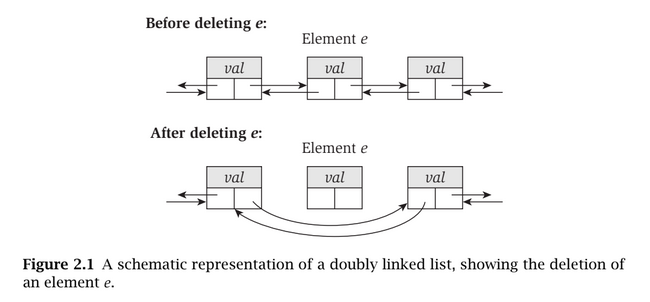
\includegraphics[width=0.8\textwidth]{Imagenes-Seccion2/fig2_1.PNG}
\end{figure}


Insertar o eliminar e al principio de la lista implica actualizar la Primera
puntero, en lugar de actualizar el registro del elemento antes e.
Si bien las listas son buenas para mantener un conjunto dinámicamente cambiante, también tienen desventajas. A diferencia de las matrices, no podemos encontrar el $i$-ésimo elemento de la lista en $O(1)$ hora: para encontrar el $i$-ésimo elemento, tenemos que seguir los siguientes punteros comenzando
desde el comienzo de la lista, que toma un tiempo total de $O(i)$.
Dadas las ventajas y desventajas relativas de las matrices y listas, puede
sucede que recibimos la entrada a un problema en uno de los dos formatos y
quiero convertirlo en el otro. Como se discutió anteriormente, tal preprocesamiento es
a menudo útil; y en este caso, es fácil convertir entre la matriz y
enumerar representaciones en $O(n)$ tiempo. Esto nos permite elegir libremente los datos
estructura que se adapte mejor al algoritmo y no se vea limitado por el camino
la información se da como entrada.\\


\subsubsection*{Implementando el algoritmo de emparejamiento estable}

A continuación, utilizaremos arreglos y listas enlazadas para implementar el algoritmo de emparejamiento estable del Capítulo 1. Ya hemos demostrado que el algoritmo termina en a lo sumo $n^2$ iteraciones, y esto proporciona un tipo de límite superior en el tiempo de ejecución. Sin embargo, si realmente queremos implementar el algoritmo G-S para que se ejecute en tiempo proporcional a $n^2$, debemos ser capaces de implementar cada iteración en tiempo constante. Discutimos cómo hacer esto ahora.\\

Para simplificar, suponga que el conjunto de hombres y mujeres son ambos $(1 ..... n)$. Para garantizar esto, podemos ordenar a los hombres y a las mujeres (por ejemplo, alfabéticamente) y asociar el número i con el i-ésimo hombre o mujer en este orden. Esta suposición (o notación) nos permite definir un arreglo indexado para todos los hombres o todas las mujeres. Necesitamos tener una lista de preferencias para cada hombre y para cada mujer. Para hacer esto tendremos dos arreglos, uno para las listas de preferencia de las mujeres y otro para las listas de preferencias de los hombres; usaremos ManPref [m, i] para denotar la i-ésima mujer en la preferencia del hombre m, y de manera similar, WomanPref [w, i] para denotar el i-ésimo hombre en la lista de preferencias de la mujer w. Tenga en cuenta que la cantidad de espacio necesaria para guardar las preferencias de todos los $2n$
individuos es $O(n^2)$, ya que cada persona tiene una lista de longitud n.\\

Necesitamos considerar cada paso del algoritmo y entender qué estructura de datos nos permite implementarlo de manera eficiente. Esencialmente, debemos ser capaces de hacer cada una de las siguientes cuatro cosas en tiempo constante (en O(1)):


\begin{itemize}
 \item Necesitamos poder identificar a un hombre libre. 
 
 \item Necesitamos, para un hombre $m$, poder identificar a la mujer mejor clasificada a quien aún no ha propuesto.
 
 \item Para una mujer $w$, debemos saber si $w$ está comprometida actualmente, y si lo está, necesitamos identificar a su pareja actual.
 
 \item Para una mujer $w$ y dos hombres $m$ y $m'$, necesitamos saber, nuevamente en tiempo constante, a cuál de los hombres prefiere $w$. \ldots 
\end{itemize}

 

Primero, seleccionamos un hombre libre. Haremos esto manteniendo el conjunto de hombres libres como una lista enlazada. Cuando necesitamos seleccionar un hombre libre, tomamos el primer hombre m en esta lista. Suprimimos a m de la lista si se compromete, y posiblemente insertamos un hombre $m’$ diferente, si algún otro hombre $m’$ queda libre. En este caso, $m'$ se puede insertar al principio de la lista, nuevamente en tiempo constante.\\

A continuación, consideramos un hombre $m$. Necesitamos identificar a la mujer mejor calificada a la que aún no ha propuesto. Para hacer esto, necesitaremos mantener un arreglo adicional, Next, que indique para cada hombre la posición de la próxima mujer a la que propondrá en su lista. Inicializamos Next[m] = 1 para todos los hombres m. Si un hombre m necesita proponerle matrimonio a una mujer, le propondrá a $w$ = ManPref $[m, Next [m]]$, y una vez que él le proponga a w, incrementaremos el valor de $Next[m]$ en uno, independientemente de si $w$ acepta o no la propuesta.\\

Ahora supongamos que el hombre m propone a la mujer w; necesitamos poder identificar al hombre m’ con quien w está comprometida (si existe tal hombre). Podemos hacer esto manteniendo un arreglo llamado actual de longitud n, donde actual [w] es el compañero actual de la mujer $w$, $m'$. Indicamos $actual[w]$ con un símbolo nulo especial cuando necesitamos indicar que la mujer w no está actualmente comprometida; al comienzo del algoritmo, $Actual[w]$ se inicializa con este símbolo nulo para todas las mujeres $w$.\\

Quizás la pregunta más difícil es cómo mantener las preferencias de las mujeres para mantener el paso (4) eficiente. Consideremos un paso del algoritmo, cuando el hombre m le propone a una mujer w. Supongamos que w ya está comprometida, y su compañero actual es $m'$ = Actual $[w]$. Nos gustaría saber en $O(1)$ si la mujer $w$ prefiere $m$ o $m'$. Mantener las preferencias de las mujeres en un arreglo WomanPref, análoga a la que usamos para los hombres, no funciona, ya que tendríamos que recorrer la lista de w uno por uno, siendo $O(n)$ el tiempo para encontrar a $m$ y $m'$ en la lista. Podemos hacerlo mucho mejor si construimos una estructura de datos auxiliar al principio.\\


Al comienzo del algoritmo, creamos una matriz $n x n$ Ranking, donde Ranking$[w, m]$ contiene el rango del hombre m en el orden de las preferencias de$w$. Mediante una única pasada a través de la lista de preferencias de $w$, podemos crear esta matriz en tiempo lineal para cada mujer, para una inversión de tiempo inicial total proporcional a $n^2$. Entonces, para decidir cuál de los hombres m o m' es preferido por w, simplemente comparamos los valores Ranking $[w, m]$ y Ranking $[w, m']$. Esto nos permite ejecutar el paso (4) en tiempo constante y, por lo tanto, tenemos todo lo que necesitamos para obtener el tiempo de ejecución deseado.\\

Las estructuras de datos descritas anteriormente nos permiten implementar el algoritmo G-S en tiempo $O(n^2)$.\\

\subsection{Una encuesta de tiempos corrientes comunes.}

Al tratar de analizar un nuevo algoritmo, ayuda a tener un sentido aproximado del "paisaje" de diferentes tiempos de ejecución. De hecho, hay estilos de análisis que se repiten con frecuencia, por lo que cuando uno ve límites de tiempo de ejecución como $O(n)$, $O(n*log n)$, y $O(n^2)$ que aparecen una y otra vez, a menudo es por un pequeño número de razones distintas. Aprender a reconocer estos estilos comunes de análisis es un objetivo a largo plazo. Para poner las cosas en marcha, ofrecemos la siguiente encuesta de los límites comunes de tiempo de ejecución y algunos de los enfoques típicos que conducen a ellos.\\

Anteriormente discutimos la noción de que la mayoría de los problemás tienen un "espacio de búsqueda": el conjunto de todas las soluciones posibles, y notamos que un tema común en el diseño de algoritmos es la búsqueda de algoritmos cuyo rendimiento sea más eficiente que una búsqueda por fuerza bruta en el espacio de búsqueda. Al acercarse a un nuevo problema, entonces, a menudo ayuda pensar en dos tipos de límites: uno en el tiempo de ejecución que se espera alcanzar, y el otro sobre el tamaño del espacio de búsqueda del problema (y por lo tanto en el tiempo de ejecución de un algoritmo por fuerza bruta para el problema). La discusión de los tiempos de ejecución en esta sección comenzará en muchos casos con un análisis del algoritmo de fuerza bruta, ya que es útil como forma de orientarse con respecto a un problema; la tarea de mejorar tales algoritmos será nuestro objetivo en la mayor parte del libro.\\

\subsubsection*{Tiempo lineal} 

Un algoritmo que se ejecuta en $O(n)$, o tiempo lineal, tiene una propiedad muy natural: su tiempo de ejecución es a lo sumo un factor constante multiplicado por el tamaño de la entrada.La forma básica de obtener un algoritmo con este tiempo de ejecución es procesar la entrada en una sola pasada, gastando una cantidad constante de tiempo en cada elemento de entrada encontrado. Otros algoritmos logran un límite de tiempo lineal por razones más sutiles. Para ilustrar algunas de las ideas aquí, consideramos dos algoritmos simples como ejemplo.\\

\subsubsection*{Calculando el máximo}

Calculando el máximo de $n$ números, por ejemplo, se puede realizar en el estilo básico "one-pass". Supongamos que los números se proporcionan como entrada en una lista o en una matriz. Procesamos los números $a_1, a_2,. . ., a_n$ en orden, manteniendo un estimado del máximo a medida que avanzamos. Cada vez que encontramos un número $a_i$, comprobamos si $a_i$ es más grande que nuestra estimación actual, y si es así, actualizamos la estimación del máximo.\\


\begin{lstlisting}
	max = a[1];
	For i = 2 to n
	If a[i] > max then
	   set max = a[i];
	   Endif
	Endfor
\end{lstlisting}

De esta forma, hacemos un trabajo constante por elemento, para un tiempo de ejecución total de $O(n)$. A veces, las restricciones de una aplicación obligan a este tipo de algoritmo, por ejemplo, un algoritmo que se ejecuta en un interruptor de alta velocidad en Internet puede ver una secuencia de paquetes que pasan volando, y puede intentarlo calculando todo lo que quiera a medida que esta corriente pasa, pero solo puede funcionar una cantidad constante de trabajo computacional en cada paquete, y no puede guardar la corriente para hacer exploraciones posteriores a través de ella.Dos subáreas diferentes de algoritmos, algoritmos en línea y algoritmos de flujo de datos, se han desarrollado para estudiar este modelo de computación.\\

\subsubsection*{Fusionando dos listas ordenadas}

A menudo, un algoritmo tiene un tiempo de ejecución de $O(n)$, pero la razón es más compleja. Ahora describimos un algoritmo para fusionar dos listas ordenadas que extiende un poco el estilo de diseño de un solo paso, pero aún así tiene un tiempo de ejecución lineal. Supongamos que nos dan dos listas de n números cada una, $ \{a_1, a_2,. . . , a_n\}$ y $\{b_1, b_2,. . . , b_n\}$, y cada uno ya está organizado en orden ascendente. A nosotros nos gustaría fusionar estos en una sola lista $\{c_1, c_2,. . . , c_{2n}\}$ que también está dispuesto en orden ascendente. Por ejemplo, combinar las listas $\{2, 3, 11, 19\}$ y $\{4, 9, 16, 25\}$ resulta en el salida $\{2, 3, 4, 9, 11, 16, 19, 25\}$. Para hacer esto, podríamos simplemente juntar las dos listas, ignorar el hecho de que se organizan por separado en orden ascendente y ejecutar un algoritmo de ordenación. Pero esto claramente parece un desperdicio; nos gustaría hacer uso del orden existente en la entrada. Una manera de pensar en diseñar un mejor algoritmo es imaginar realizar la fusión de las dos listas a mano: supongamos que te dan dos montones de tarjetas numeradas, cada una ordenada en orden ascendente, y le gustaría producir una sola pila ordenada que contenga todas las cartas. Si miramos la tarjeta superior en cada pila, sabemos que el más pequeño de estos dos debería ir primero en la pila de salida; quitamos esta tarjeta, la colocamos en la salida y ahora iteramos en lo que queda. En otras palabras, tenemos el siguiente algoritmo.\\

\begin{lstlisting}
	Para combinar listas ordenadas A = a[1],. . . , a[n] y B = b[1],. . . , b[n]:
      Mantenga un puntero actual en cada lista, inicializado en los elementos frontales;
      While Si ambas listas no son vacias:
         Deje que a[i] y b[j] sean los elementos senalados por el puntero actual;
         Adjunte el mas pequeno de estos dos a la lista de salida;
         Avance el punterio actual de la lista de donde fue seleccionado el elemento;
      EndWhile
      Cuando una lista quede vacia, se agrega el resto de la otra a la salida;
\end{lstlisting}



\begin{figure}[h] 
  \centering
    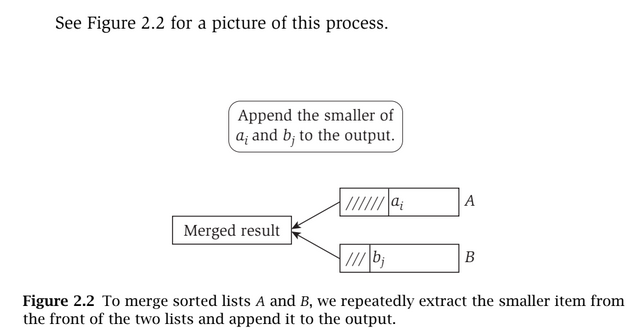
\includegraphics[width=0.8\textwidth]{Imagenes-Seccion2/fig2_2_real.PNG}
\end{figure}


Ahora, para mostrar un límite de tiempo lineal, uno tiene la tentación de describir un argumento como lo que funcionó para el algoritmo de búsqueda del máximo: "Hacemos un trabajo constante por elemento, para un tiempo de ejecución total de $O(n)$." Pero en realidad no es cierto que hacemos solo un trabajo constante por elemento. Supongamos que $n$ es un número par, y considere las listas $A =\{ 1, 3, 5,. . . , 2n-1\}$ y $B =\{ n, n + 2, n + 4,. . . , 3n-2 \}$. El número $b_1$ en el frente de la lista B se ubicará al principio de la lista durante $n / 2$ iteraciones mientras que los elementos de A se seleccionan repetidamente, y por lo tanto estará involucrado en $\Omega(n)$ comparaciones. Ahora bien, es cierto que cada elemento puede participar en la mayoría de las comparaciones de $O(n)$ (en el peor de los casos, se compara con cada elemento en la otra lista), y si sumamos esto sobre todos los elementos obtenemos un límite de $O(n^2)$ en tiempo de ejecución. Este es un límite correcto, pero podemos mostrar algo mucho más fuerte.\\

La mejor manera de argumentar es limitar el número de iteraciones del While por un esquema de "contabilidad". Supongamos que cobramos el costo de cada iteración al elemento que se selecciona y agrega a la lista de salida. A cada elemento se le cobrará solo una vez, ya que en el momento en que se carga por primera vez, se agrega a la salida y no se vuelve a visitar por el algoritmo. Pero solo hay $2n$ total de elementos, y el costo de cada iteración se explica por un cargo a algún elemento, por lo que puede haber como máximo $2*n$ iteraciones. Cada iteración implica una cantidad constante de trabajo, por lo que el tiempo total de ejecución es $O(n)$, según lo deseado.\\

 Mientras este algoritmo de fusión iteraba a través de sus listas de entrada en orden,La forma "intercalada" en la que procesaba las listas requería un análisis  sutil del tiempo de ejecución. En el Capítulo 3 veremos algoritmos de tiempo lineal para grafos que tienen un flujo de control aún más complejo: gastan una cantidad constante de tiempo en cada nodo y arista subyacente en el grafo, pero el orden en el que procesan los nodos y las aristas depende de la estructura del grafo.\\

\subsubsection*{Tiempo $O(nlogn)$} 

$O(nlog n)$ también es un tiempo de ejecución común, y en el Capítulo 5 veremos uno de los principales motivos de su prevalencia: es el tiempo de ejecución de cualquier algoritmo que divide su entrada en dos piezas de igual tamaño, resuelve cada pieza recursivamente, y luego combina las dos soluciones en tiempo lineal.\\

La clasificación es quizás el ejemplo más conocido de un problema que puede ser resuelto de esta manera. Específicamente, el algoritmo Mergesort divide el conjunto de números de entrada en dos pedazos de igual tamaño, ordena cada mitad recursivamente, y luego fusiona las dos mitades ordenadas en una sola lista de salida ordenada. Acabamos de ver que la fusión se puede hacer en tiempo lineal; y en el Capítulo 5 discutiremos cómo analizar la recursión para obtener un límite de $O(n*log n)$ en el tiempo de ejecución.\\

Uno también encuentra con frecuencia $O(n*log n)$ como un tiempo de ejecución simplemente, porque hay muchos algoritmos cuyo paso más caro es ordenar la entrada. Por ejemplo, supongamos que se nos da un conjunto de $n$ marcas de tiempo $x_1, x_2,. . . , x_n$ en que copias de un archivo llegaron a un servidor, y nos gustaría encontrar el más grande intervalo de tiempo entre la primera y la última de estas marcas de tiempo durante las cuales no llego ninguna copia del archivo. Una solución simple a este problema es primero ordenar el sellos de tiempo $x_1, x_2,. . . , x_n$ y luego procesarlos en orden, determinando los tamaños de las brechas entre cada número y su sucesor en orden ascendente. La mayor de estas brechas es el subintervalo deseado. Tenga en cuenta que este algoritmo requiere $O(n*log n)$ tiempo para ordenar los números, y luego gasta tiempo constante en trabajar en cada número en orden ascendente. En otras palabras, el resto de la algoritmo después de la clasificación sigue la receta básica para el tiempo lineal que discutimos más temprano.\\

\subsubsection*{Tiempo cuadrático} 
Aquí hay un problema básico: supongamos que le dan $n$ puntos en el plano, cada uno especificado por coordenadas $(x,y)$, y le gustaría encontrar el par de puntos que están más cerca entre sí. El algoritmo de fuerza bruta natural para este problema enumeraría todos los pares de puntos, calcularía la distancia entre cada par, y luego elegiría el par para el que esta distancia es más pequeña.\\

¿Cuál es el tiempo de ejecución de este algoritmo? El número de pares de puntos es $C(n,2)=n(n-1)/2$, y dado que esta cantidad está limitada por $(1/2)(n^2)$, es $O(n^2)$. Más crudamente, el número de pares es $O(n^2)$ porque multiplicamos el número de formás de elegir el primer miembro del par (a lo sumo $n$) por el número de formás de elegir el segundo miembro del par (también en la mayoría $n$). La distancia entre los puntos \((x_{i},y_{i})\) y \((x_{j},y_{j})\) Se puede calcular mediante la fórmula
\(\sqrt{(x_{i}-x_{j})^2+(y_{i}-y_{j})^2}\) en tiempo constante, por lo que el tiempo total de ejecución es $O(n^2)$. Este ejemplo ilustra una forma muy común en la que surge un tiempo de ejecución de $O(n^2)$: realizar una búsqueda sobre todos los pares de elementos de entrada y gastar un tiempo constante por par.\\

El tiempo cuadrático también surge naturalmente de un par de bucles anidados: un algoritmo consiste en un bucle con iteraciones $O(n)$, y cada iteración del bucle inicia un bucle interno que toma $O(n)$ el tiempo. Al multiplicar estos dos factores de n, se obtiene el tiempo de ejecución. 
El algoritmo de fuerza bruta para encontrar el par de puntos más cercano se puede escribir de manera equivalente con dos bucles anidados:\\


\begin{lstlisting}
   For cada punto de entrada (xi, yi)
     For cada otro punto de entrada (xj, yj)
       Computar distancia d=sqrt((xi-xj)^2+(yi-yj)^2)
           Si d es menor que el minimo actual, actualice el minimo a d
     Endfor
   Endfor
\end{lstlisting}

Observe cómo el bucle "interno", sobre $(xj,yj)$, tiene iteraciones $O(n)$, cada una de las cuales toma un tiempo constante; y el bucle "externo", sobre $(xi,yi)$, tiene $O(n)$ iteraciones, cada una invocando el bucle interno una vez.\\

Es importante notar que el algoritmo que hemos estado discutiendo para el problema del par más cercano realmente es solo el enfoque de fuerza bruta: el espacio de búsqueda natural para este problema tiene el tamaño $O(n^2)$, y simplemente lo estamos enumerando. Al principio, uno siente que hay una cierta inevitabilidad sobre este algoritmo cuadrático, tenemos que medir todas las distancias, ¿no? Pero de hecho esto es una ilusión. En el Capítulo 5 describimos un algoritmo muy inteligente que encuentra el par de puntos más cercano en el plano en solo $O(nlogn)$ tiempo, y en el Capítulo 13 mostramos cómo se puede usar la aleatorización para reducir el tiempo de ejecución a $O(n)$.\\

\subsubsection*{Tiempo cúbico} 

Conjuntos más elaborados de bucles anidados a menudo conducen a algoritmos que se ejecutan en tiempo $O(n3)$. Considere, por ejemplo, el siguiente problema. Nos dan conjuntos $S1, S2, ..., Sn$, cada uno de los cuales es un subconjunto de ${1, 2,. . . , n}$, y nos gustaría saber si algún par de estos conjuntos es disjunto; en otras palabras, no tiene elementos en común.\\

¿Cuál es el tiempo de ejecución necesario para resolver este problema? Supongamos que cada conjunto $Si$ está representado de tal manera que los elementos de $Si$ se pueden enumerar en tiempo constante por elemento, y también podemos verificar en tiempo constante $si$ un número dado p pertenece a $Si$. La siguiente es una forma directa de abordar el problema.\\


\begin{lstlisting}
For par de conjuntos S[i] y S[j]
    Determine si S[i] y S[j] tienen un elemento en comun
Endfor
\end{lstlisting}
\paragraph{}
Este es un algoritmo concreto, pero razonar sobre su tiempo de ejecución ayuda a
abrirlo (al menos conceptualmente) en tres bucles anidados.\\

\begin{lstlisting}
For each set S[i]
  For each other set S[j]
    For each element p of S[i]
      Determine whether p also belongs to S[j]
    Endfor
    If no element of Si belongs to S[j] then
      Report that S[i] and S[j] are disjoint
    Endif
  Endfor
Endfor
\end{lstlisting}
\paragraph{}
Cada uno de los conjuntos tiene un tamaño máximo $O(n)$, por lo que el ciclo más interno toma tiempo $O(n)$. Looping sobre los conjuntos Sj implica $O(n)$ iteraciones alrededor de este ciclo más interno; y haciendo un bucle sobre los conjuntos Si implica $O(n)$ iteraciones alrededor de esto. Al multiplicar estos tres factores de $n$ juntos, obtenemos el tiempo de ejecución de $O(n3)$. Para este problema, existen algoritmos que mejoran el tiempo de ejecución $O(n3)$, pero son bastante complicados. Además, no está claro si los algoritmos mejorados para este problema son prácticos en entradas de tamaño razonable.\\

\subsubsection*{Tiempo $O(n^k)$} 

Del mismo modo que obtuvimos un tiempo de ejecución de $O(n^2)$ realizando una búsqueda de fuerza bruta sobre todos los pares formados a partir de un conjunto de $n$ elementos, obtenemos un tiempo de ejecución de $O(n^k)$ para cualquier constante $k$ cuando buscamos todos los subconjuntos de tamaño k.\\

Considere, por ejemplo, el problema de encontrar conjuntos independientes en un grafo, que discutimos en el Capítulo 1. Recuerde que un conjunto de nodos es independiente si no hay dos unidos por una arista. Supongamos, en particular, que para una constante fija $k$, nos gustaría saber si un grafo de entrada $n$ dado nodo $G$ tiene un conjunto independiente de tamaño $k$. El algoritmo natural de fuerza bruta para este problema enumeraría todos los subconjuntos de $k$ nodos, y para cada subconjunto $S$ verificaría si hay una arista que une a dos miembros de $S$. Es decir, \\
\paragraph{}
\begin{lstlisting}
For each subset S of k nodes
	Check whether S constitutes an independent set
      If S is an independent set 
          then Stop and declare success
      Endif
Endfor
If no k-node independent set was found 
	then Declare failure
Endif
\end{lstlisting}
\paragraph{}

Para comprender el tiempo de ejecución de este algoritmo, debemos considerar dos cantidades. Primero, el número total de subconjuntos de elementos $k$ en un conjunto de $n$ elementos es\\



\begin{figure}[h] 
  \centering
    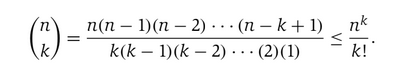
\includegraphics[width=0.5\textwidth]{Imagenes-Seccion2/form_2_3.PNG}
\end{figure}


Como estamos tratando k como una constante, esta cantidad es $O(n^k)$. Por lo tanto, el bucle externo en el algoritmo anterior se ejecutará para iteraciones $O(n^k)$ ya que prueba todos los subconjuntos k-nodos de los n nodos del grafo.\\

Dentro de este ciclo, necesitamos probar si un conjunto dado $S$ de $k$ nodos constituye un conjunto independiente. La definición de un conjunto independiente nos dice que debemos verificar, para cada par de nodos, si hay una arista que los une. Por lo tanto, esta es una búsqueda sobre pares, como vimos anteriormente en la discusión del tiempo cuadrático; requiere mirar $C(k,2)$, es decir, $O(k^2)$, pares y pasar tiempo constante en cada uno.\\

Por lo tanto, el tiempo total de ejecución es $O(k^2.n^k)$. Dado que estamos tratando $k$ como una constante aquí, y dado que las constantes se pueden eliminar en notación $O(·)$, podemos escribir este tiempo de ejecución como $O(n^k)$.\\

El conjunto independiente es un ejemplo principal de un problema que se cree que es
computacionalmente difícil, y en particular se cree que ningún algoritmo para encontrar conjuntos independientes de $k$-nodos en grafos arbitrarios puede evitar tener cierta dependencia de $k$ en el exponente. Sin embargo, como discutiremos en el Capítulo 10 en el contexto de un problema relacionado, incluso una vez que hayamos admitido que la búsqueda de fuerza bruta sobre los subconjuntos de $k$-elementos es necesaria, puede haber diferentes formás de resolver esto que conducen a diferencias significativas en la eficiencia del cálculo.\\


\subsubsection*{Más allá del tiempo polinómico} 

El ejemplo anterior del problema del conjunto independiente nos inicia rápidamente en el camino hacia tiempos de ejecución que crecen más rápido que cualquier polinomio. En particular, dos tipos de límites que surgen con mucha frecuencia son 2n y n!, y ahora discutimos por qué esto es así.\\

Supongamos, por ejemplo, que se nos da un grafo y queremos encontrar un conjunto independiente de tamaño máximo (en lugar de probar la existencia de uno con un número dado de nodos). Nuevamente, las personas no conocen los algoritmos que mejoran significativamente en la búsqueda de fuerza bruta, que en este caso se vería de la siguiente manera.
 
\begin{lstlisting}
For each subset S of nodes
	Check whether S constitutes an independent set
	If S is a larger independent set than the largest seen so far then
		Record the size of S as the current maximum
	Endif
Endfor
\end{lstlisting}

Esto es muy parecido al algoritmo de fuerza bruta para conjuntos independientes de k-nodos, excepto que ahora estamos iterando sobre todos los subconjuntos del grafo. El número total de subconjuntos de un conjunto de n elementos es $2^n$, y por lo tanto, el bucle externo en este algoritmo se ejecutará durante 2n iteraciones mientras intenta todos estos subconjuntos. Dentro del ciclo, estamos comprobar todos los pares de un conjunto S que puede ser tan grande como n nodos, por lo que cada iteración del
ciclo toma como máximo $O(n^2)$ tiempo. Al multiplicar estos dos, obtenemos un tiempo de ejecución de $O(n^2.2^n)$.\\

Por lo tanto, vea que $2^n$ surge naturalmente como un tiempo de ejecución para un algoritmo de búsqueda que debe considerar todos los subconjuntos. En el caso de Independent Set, algo al menos casi este ineficiente parece ser necesario; pero es importante tener en cuenta que $2^n$ es el tamaño del espacio de búsqueda para muchos problemás, y para muchos de ellos podremos encontrar polinomios tiempo altamente eficiente algoritmos. Por ejemplo, un algoritmo de búsqueda de fuerza bruta para el
Intervalo Problema de programación que vimos en el Capítulo 1 sería muy similar al Algoritmo anterior: pruebe todos los subconjuntos de intervalos, y encuentre el subconjunto más grande que tiene no se superpone. Pero en el caso del problema de programación de intervalos, en contraposición al problema del conjunto independiente, veremos (en el Capítulo 4) cómo encontrar una solución óptima en el tiempo $O(n log n)$. Este es un tipo recurrente de dicotomía en el estudio de algoritmos: dos algoritmos pueden tener una búsqueda muy similar espacios, pero en un caso puede eludir el algoritmo de búsqueda de fuerza bruta, y en el otro no lo es.\\

La función $n!$ crece incluso más rápido que $2^n$, por lo que es aún más amenazante como un límite en el rendimiento de un algoritmo. Buscar espacios de tamaño $n!$ tienden a surgir por una de dos razones. ¡Primero $N$! es la cantidad de formás de unir $n$ elementos con $n$ otros elementos; por ejemplo, es el número de posibles emparejamientos perfectos de $n$ hombres con n mujeres en un ejemplo del apareamiento estable Problema. Para ver esto, tenga en cuenta que hay $n$ opciones de cómo podemos hacer coincidir El primer hombre; habiendo eliminado esta opción, hay $n-1$ opciones de cómo puede coincidir con el segundo hombre; habiendo eliminado estas dos opciones, hay $n-2$ elecciones de cómo podemos emparejar al tercer hombre; Etcétera. Multiplicando todas estas opciones, obtenemos $n(n-1)(n-2)...(2)(1)=n!$\\

A pesar de este enorme conjunto de posibles soluciones, pudimos resolver el problema de apareamiento estable en $O(n^2)$ iteraciones del algoritmo de propuesta.
En el Capítulo 7, veremos un fenómeno similar para la adaptación bipartita Problema que discutimos anteriormente; si hay n nodos en cada lado del dado grafo bipartito, puede haber hasta n! formás de emparejarlos. Sin embargo, por un algoritmo de búsqueda bastante sutil, podremos encontrar el bipartito más grande coincidencia en el tiempo $O(n^3)$.\\

La función $n!$ también surge en problemás donde el espacio de búsqueda consiste
de todas las maneras de organizar $n$ elementos en orden. Un problema básico en este género es el Problema del vendedor ambulante: dado un conjunto de $n$ ciudades, con distancias entre todas las parejas, ¿cuál es el recorrido más corto que visita todas las ciudades? Suponemos que el el vendedor comienza y termina en la primera ciudad, entonces el quid del problema es la búsqueda implícita sobre todos los pedidos de las restantes $n-1$ ciudades, lo que lleva a un espacio de búsqueda de tamaño $(n-1)!$. En el Capítulo 8, veremos que Traveling Salesman es otro problema que, como Independent Set, pertenece a la clase de problemás NP-complete y se cree que no tiene una solución
eficiente.\\

\subsubsection*{Tiempo sublineal}

Finalmente, hay casos en los que uno encuentra tiempos de ejecución que son asintóticamente más
pequeños que lineales. Dado que toma tiempo lineal solo leer la entrada, estas situaciones tienden a
surgir en un modelo de computación donde la entrada se puede "consultar" indirectamente en lugar de
leer por completo, y el objetivo es minimizar la cantidad de consultas que se deben hacer.\\

Quizás el ejemplo más conocido de esto es el algoritmo de búsqueda binaria. Dada una matriz
ordenada A de n números, nos gustaría determinar si un número dado p pertenece a la matriz.
Podríamos hacer esto leyendo toda la matriz, pero nos gustaría hacerlo de manera mucho más
eficiente, aprovechando el hecho de que la matriz está ordenada, probando cuidadosamente las
entradas particulares. En particular, sondeamos la entrada del medio de A y obtenemos su valor,
digamos que es q, y comparamos q con p. Si q = p, hemos terminado. Si $q>p$, entonces para que p
pertenezca a la matriz A, debe estar en la mitad inferior de A; entonces ignoramos la mitad superior de
A
ahora y aplicar recursivamente esta búsqueda en la mitad inferior. Finalmente, si $q<p$, entonces
aplicamos el razonamiento análogo y la búsqueda recursiva en la mitad superior de A.\\

El punto es que, en cada paso, hay una región de A donde posiblemente podría estar p; y
estamos reduciendo el tamaño de esta región en un factor de dos con cada sonda. Entonces, ¿cuán grande es la región "activa" de las sondas A después de k? Comienza en tamaño n, por lo que después de k sondas tiene un tamaño máximo de $n(1/2)^k$.\\

Dado esto, ¿cuánto tiempo tomará para que el tamaño de la región activa se reduzca a una
constante? Necesitamos que k sea lo suficientemente grande para que $(1/2)^k=O(1/n)$, y para hacer
esto podemos elegir $k=log n$. Por lo tanto, cuando $k=log n$, el tamaño de la región activa se ha
reducido a una constante, en cuyo punto la recursión toca fondo y podemos buscar el resto de la matriz
directamente en tiempo constante.\\

Por lo tanto, el tiempo de ejecución de la búsqueda binaria es $O(log n)$, debido a esta
contracción sucesiva de la región de búsqueda. En general, $O(log n)$ surge como un límite de tiempo
siempre que se trata de un algoritmo que realiza una cantidad constante de trabajo para descartar una
fracción constante de la entrada. El hecho crucial es que $O(log n)$ tales iteraciones son suficientes para
reducir la entrada a un tamaño constante, en cuyo punto el problema generalmente se puede resolver
directamente\\


\subsection{Ejercicios resueltos}

\subsubsection*{Ejercicio 1} 

Tome la siguiente lista de funciones y organícelas en orden ascendente según la tasa de crecimiento. Es decir, si la función $g(n)$ sigue inmediatamente a la función $f(n)$ en su lista, entonces debería ser el caso de que $f(n)$ sea $O(g(n))$.\\

\begin{figure}[h] 
  \centering
    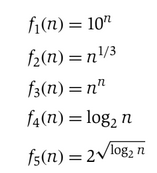
\includegraphics[width=0.2\textwidth]{Imagenes-Seccion2/form2_1.PNG}
\end{figure}

\textbf{Solución} Podemos tratar las funciones $f_1$,$ f_2$ y $f_4$ muy fácilmente, ya que pertenecen a las familias básicas de exponenciales, polinomios y logaritmos. En particular, por (2.8), tenemos $f_4 (n) = O (f_2 (n))$; y por (2.9), tenemos $f_2 (n) = O (f_1 (n))$.\\

Ahora, la función $f_3$ no es tan difícil de tratar. Comienza a partir de $10 ^ n$, pero una vez $n ≥ 10$, entonces claramente $10 ^ n ≤ n ^ n$. Esto es exactamente lo que necesitamos para la definición de la notación $O (·)$: para todo $n ≥ 10$, tenemos $10 ^ n ≤ cn ^ n$, donde en este caso $c = 1$, y entonces $10 ^ n = O (n ^ n)$.\\

Finalmente, llegamos a la función $f_5$, que es ciertamente algo extraño. Una regla práctica útil en tales situaciones es tratar de tomar logaritmos para ver si esto aclara las cosas. En este caso, $log_2 f_5 (n) = sqrt (log_2 n) = (log_2 n) ^ (1/2)$. ¿A qué se parecen los logaritmos de las otras funciones? $log f_4 (n) = log_2 log_2 n$, mientras que $log f_2 (n) = (1/3) log_2 n$. Todos estos pueden ser vistos como funciones de $log_2 n$, y entonces usando la notación $z = log2_n$, podemos escribir .

\begin{figure}[h] 
  \centering
    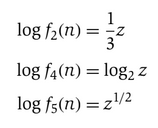
\includegraphics[width=0.2\textwidth]{Imagenes-Seccion2/form2_2.PNG}
\end{figure}

Ahora es más fácil ver qué está pasando. Primero, para $z ≥ 16$, tenemos $log_2 z ≤  z$  $^1$ $^/$ $^2$. Pero la condición $z ≥ 16$ es igual que $n ≥ 216 = 65, 536$; por lo tanto, una vez $n ≥ 2 ^1$ $^6$ tenemos $log f_4 (n) ≤ log f_5 (n)$, y así $f_4 (n) ≤ f_5 (n)$. Por lo tanto, podemos escribir $f_4 (n) = O (f_5 (n))$. Similarmente, tenemos $z^1$ $^/$ $^ 2$ $≤ (1/3)z$ una vez $z ≥ 9$ -en otras palabras, una vez $n ≥ 29 = 512$. Para n arriba de este límite tenemos $log f_5 (n) ≤ log f_2 (n)$ y por lo tanto $f_5 (n) ≤ f_2 (n)$, y entonces podemos escribir $f_5 (n) = O (f_2 (n))$. Esencialmente, hemos descubierto que $2$ $\sqrt log_2 (n))$ es una función cuya tasa de crecimiento se encuentra en algún lugar entre la de los logaritmos y polinomios.\\

\subsubsection*{Ejercicio 2} 

Sean $f$ y $g$ dos funciones que toman valores no negativos, y supongamos que $f=O(g)$. Muestre que $g=\Omega(f)$.\\\\
\textbf{Solución} Este ejercicio es una manera de formalizar la intuición de que $O(.)$ y $\Omega(·)$ son en cierto sentido opuestos. De hecho, no es difícil de probar; es solo cuestión de deshacer las definiciones.\\
Se nos da que, para algunas constantes $c$ y $n0$, tenemos $f(n)≤cg(n)$ para todo $n≥n0$. Dividiendo ambos lados por $c$, podemos concluir que $g(n)≥(1/c).f(n)$ para todo $n≥n0$. Pero esto es exactamente lo que se requiere para demostrar que $g=\Omega(f)$: hemos establecido que $g(n)$ es al menos un múltiplo constante de $f(n)$ (donde la constante es $1/c$), para todos los suficientemente grandes $n$ (al menos $n0$).\\


\newpage
\section{Grafos}

Nuestro enfoque en este libro sera sobre problemás en los cuales se puedan utilizar herramientas de matemática discreta. Las matemáticas en espacios continuas han desarrollado ciertas estructuras básicas como números reales, vectores y matrices, sin embargo las matemáticas discretas han desarrollado la combinatoria, las cuales son unas estructuras que se encuentran en el corazón del tema. Uno de las estructuras más fundamentales y visuales de esta son los grafos. \\

Mientras más se trabaja con grafos, más se tiende a verlos en todas partes.
Por lo tanto, comenzamos por introducir las definiciones básicas sobre los grafos, también enumeraremos diferentes configuraciones algorítmicas donde intuitivamente pueden interpretarse como grafos. Luego discutiremos algunos algoritmos básicos para grafos, comenzando
con el problema de la conexión y el desarrollo de algunas técnicas fundamentales de búsqueda en grafos.\\

\subsection{Definiciones básicas y aplicaciones}

Recuerde del Capítulo 1 que un grafo $G$ es simplemente una forma de codificar por pares las
relaciones entre un conjunto de objetos: La misma consiste en un conjunto $V$ de nodos
y un conjunto $E$ de aristas, las cuales "unen" dos nodos. Por lo tanto
representaremos una arista $e \in E$ como un subconjunto de dos elementos de $V$: $e = \{u, v\}$ para algún $u, v \in V$.  Entonces dada una arista  $e = \{u, v\}$ a los nodos $u$ y $v$ los llamaremos vértices de $e$.\\

Las aristas de un grafo indican una relación simétrica entre sus extremos.
A menudo queremos codificar relaciones asimétricas, y para esto usamos la
noción de grafo dirigido. Un grafo dirigido $G^{'}$ consiste en un conjunto
de nodos $V$ y un conjunto de aristas dirigidas $E^{'}$.  Cada $e^{'} \in E^{'}$ es un par ordenado $(u, v)$; en otras palabras, los roles de $u$ y $v$ no son intercambiables,   denominaremos cola de la arista al vértice $u$ y a $v$ le llamaremos la cabeza de $e$. Aveces, también diremos que la arista $e^{'}$ sale del nodo $u$ y entra en el nodo $v$. \\

Por defecto, en este libro cuando hagamos referencia a un grafo, estaremos haciendo referencia a un grafo no dirigido. También vale la pena mencionar dos advertencia sobre nuestro uso en la terminología de grafos. Primero, aunque una arista $e$ en un grafo no dirigido debe escribirse correctamente como un conjunto de nodos $\{u, v\}$,  a menudo uno lo verá escrito (incluso en este libro) con la notación utilizada para pares ordenados: $e = (u,v)$. En segundo lugar, a los nodos de un grafo se les denomina frecuentemente como vértices; en este contexto, las dos palabras tienen exactamente el mismo significado.  \\

\textbf{Ejemplos de grafo:} Los grafos son muy simples de definir: simplemente tomamos una colección
de vértices y unimos a algunos de ellos mediante líneas. Pero en este nivel de abstracción,
es difícil apreciar las típicas situaciones que pueden modelarse mediante ellos. Por lo cual, a continuación daremos una lista de situaciones donde los grafos juegan un papel fundamental en su modelado. La lista es muy amplia, y no es importante recordarla toda; más bien, nos proporcionará muchos ejemplos útiles con los cuales podremos verificar las definiciones básicas y problemás algorítmicos que encontraremos más adelante en el capítulo. Además, al dar esta lista, se podrá entender mejor el significado de los nodos y el significado de las aristas en
el contexto del modelado y aplicación de los grafos. En algunos casos, los nodos y aristas se corresponden a objetos físicos del mundo real, en otros los nodos son objetos reales
mientras que las aristas son virtuales, y en otros, tanto los nodos como las aristas son puros
abstracciones. \\

\begin{enumerate}
\item \textbf{Redes de transporte:} El mapa de las rutas realizadas por aviones de una aerolínea forma naturalmente un grafo: los nodos son aeropuertos y la arista $(u,v)$ pertenece al grafo si hay un vuelo sin escalas que parte de $u$ y arriba a $v$. Descrita de esta manera, el grafo está dirigido; pero en la realidad cuando hay una arista $(u,v)$ casi siempre también hay una $(v,u)$, así que lo supondremos, ya que no perdemos demásiado si tratamos el mapa de rutas de la aerolínea como un grafo no dirigido con aristas que unen pares de aeropuertos que tienen vuelos sin escalas en cada sentido. Mirando el grafo (por lo general, se pueden encontrar grafos de este tipo en revistas de aeronáutica), notamos rápidamente algunas cosas: a menudo se pueden observar que existen vértices con una cantidad de aristas incidentes mayor al promedio; y además, dados dos nodos del grafo, es posible llegar de uno al otro, pasando por pocos vértices intermedios. \\

Otras redes de transporte se pueden modelar de manera similar. Por
ejemplo, podríamos tomar una red ferroviaria y tener un nodo para cada terminal,
y una arista que une $(u,v)$ si hay una vía férrea que va entre ellos sin detenerse en ninguna terminal intermedia. La representación estándar del mapa del metro en una ciudad importante es un dibujo de un grafo. \\

\item \textbf{Redes de comunicación:} Un grupo de computadoras conectadas a través de
una red de comunicación se puede modelar de forma natural con un grafo, existen diferentes formás de hacerlo. Primero, podríamos tener un nodo para cada computadora y
una arista que une $u$ y $v$ si hay un enlace físico directo que las conecta. Alternativamente, para estudiar estructuras a gran escala como Internet,
las personas a menudo definen un nodo como el conjunto de todas las máquinas controladas por un solo proveedor de servicios de Internet, y una arista que une $u$ y $v$ si hay una relación directa de conexión entre ellas, en otras palabras si existe un acuerdo para intercambiar datos bajo el protocolo estándar BGP que gobierna de forma global el Enrutamiento de Internet. Tenga en cuenta que esta última red es más "virtual" que la primera, ya que los enlaces indican un acuerdo formal además de
una conexión física.\\

Al estudiar las redes inalámbricas, uno típicamente define un grafo donde
los nodos son dispositivos de computación situados en ubicaciones en el espacio físico,
y hay una arista de $u$ a $v$ si $v$ está lo suficientemente cerca como para recibir una señal del dispositivo de red inalámbrica. Tenga en cuenta que a menudo es útil ver esta situacion de esta forma (como un grafo dirigido), ya que puede darse el caso de que $v$ pueda recibir tu señal pero no puedas recibir la señal de $v$
(si, por ejemplo, $u$ tiene un transmisor más fuerte). Estos grafo también son
interesante desde una perspectiva geométrica, ya que corresponden aproximadamente
a poner puntos en el plano y luego unir los pares de vértices que están cerca. \\

\item \textbf{Redes de información:}
La World Wide Web (red informática mundial) se puede ver naturalmente como un grafo dirigido, en el que los nodos corresponden a páginas web y hay una
arista de $u$ a $v$ si $u$ tiene un hipervínculo (enlace) a $v$. La dirección del grafo es crucial aquí; muchas páginas, por ejemplo, enlazan a sitios de noticias populares,
pero estos sitios claramente no corresponden a todos estos enlaces. La estructura de
todos estos hipervínculos pueden ser utilizados por algoritmos (como el de google) para tratar de inferir cuales son las páginas más importantes en la web, esta es una técnica empleada por la mayoría de los motores de búsqueda actuales.\\

La estructura de hipervínculos de la web es precedida por redes de información que surgieron muchas décadas antes. Entre las redes que la preceden se encuentran las redes de citación biográfica de informes científicos.
\item \textbf{Redes de sociales:}
Dada un conjunto de personas que interactúan entre si (los empleados
de una compañía, los estudiantes en una escuela secundaria o los habitantes de
un pueblo pequeño), podemos definir una red cuyos nodos son personas, con
una arista que une $u$ y $v$ si son amigos entre sí. Podríamos
definir las aristas con otros significados en lugar de amistad:
por ejemplo la arista no dirigida $(u, v)$ podría significar que $u$ y $v$ han tenido una relación romántica o una relación financiera; la arista dirigida $(u, v)$ podría
 decir que $u$ busca consejo de $v$, o que $u$ tiene a $v$ en su lista de correo electrónico. También se pueden imaginar redes sociales bipartitas basadas en una noción de afiliación: dado un conjunto $X$ de personas y un conjunto $Y$ de organizaciones,
podríamos definir una entre $u \in X$ y $v \in Y$ si la persona $u$ pertenece
a la organización $v$.
Redes como esta son usadas ampliamente por los sociólogos para estudiar
la dinámica de la interacción entre las personas. Se pueden usar para identificar
las personas más "influyentes" en una empresa u organización, para modelar
la confianza en las relaciones en un contexto financiero o político, y seguir la propagación de modas, rumores, bromás, enfermedades y virus de correo electrónico.
\item \textbf{Redes de dependencia:} 
Es natural definir grafo dirigidos que capturen
las dependencias entre un conjunto de objetos. Por ejemplo, dada la lista de cursos ofrecidos por un colegio o universidad, podríamos tener un nodo para cada curso y una arista de $u$ a $v$ si $u$ es previa de $v$. (Véase grafo de previas de ingeniería en computación - Udelar) Dada una lista de funciones o módulos en un gran sistema de software, podríamos tener un nodo para cada función y una arista de $u$ a $v$ si $u$ invoca a $v$ por una llamada a la función. O dado un conjunto de especies en un ecosistema, podríamos definir un grafo de una red alimentaria en el que los nodos son las diferentes especies y hay una arista de $u$ a $v$ si $u$ consume $v$.
\end{enumerate}
Esto está lejos de ser una lista completa, demásiado lejos para siquiera comenzar a escribir. Simplemente se trata de sugerir algunos ejemplos que son útiles para tener en cuenta cuando comencemos a pensar en grafos en un contexto algorítmico.\\

\textbf{Caminos y conectividad:} Una de las operaciones fundamentales en un grafo es
el de recorrer una secuencia de nodos conectados por las aristas. En los ejemplos
que acabamos de enumerar, un cruce de este tipo podría corresponder a un usuario que navega por páginas web siguiendo hipervínculos; un rumor que pasa de boca en boca de usted a alguien a través de todo el mundo; o un pasajero de una aerolínea que viaja desde San Francisco a Roma en una secuencia de vuelos.

Con esta idea en mente, definimos un camino en un grafo no dirigido
$G = (V, E)$ como una secuencia $P$ de nodos $v_1, v_2, ..., v_{k-1},v_k$ con la propiedad de que cada par consecutivo $v_i, v_{i+1}$ está unido por una arista en $G$. A menudo se dice que $P$ es un camino de $v_1$ a $v_k$, o un camino $v_1-v_k$. Por ejemplo, los nodos 4, 2, 1, 7, 8 forman un camino en la Figura 3.1. Se dice que un camino es un camino simple si todos sus vértices son distintos. Un ciclo es un camino $v_1, v_2, ..., v_{k-1}, v_k$ en el cual $k> 2$, y los primero $k-1$
 nodos son todos distintos, y $v_1 = v_k$; en otras palabras, la secuencia de nodos
"regresa" al punto de partida. Todas estas definiciones se heredan naturalmente
a los grafos dirigidos, con el siguiente cambio: en un camino o ciclo dirigido,
cada par de nodos consecutivos tiene la propiedad de que $(v_i, v_{i+1})$ es una arista. En otras palabras, la secuencia de nodos en el camino o ciclo debe respetar el direccionalidad de las aristas.\\

\begin{figure}[h]
\centering
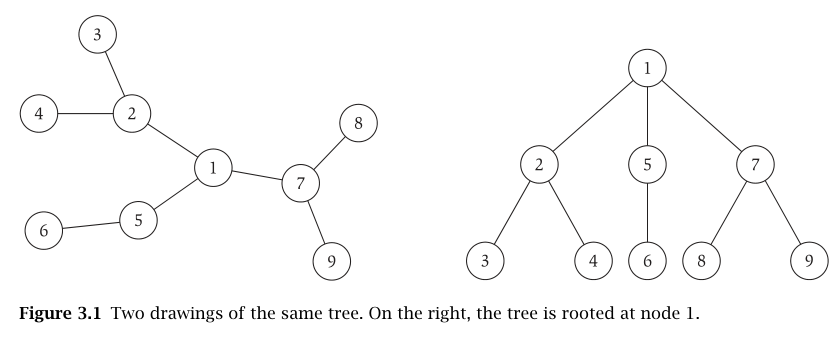
\includegraphics[width=1\textwidth]{Imagenes-Seccion3/fig3_1.PNG}
\caption{ }
 \label{fig:Imagenes-Seccion3/fig3_1.PNG}
\end{figure}

Decimos que un grafo no dirigido es conexo si, por cada par de nodos $u,v$, existe un camino desde $u$ hasta $v$. Elegir cómo definir la conectividad de un  grafo dirigido es un poco más sutil, ya que es posible que tengas un camino desde $u$ hacia $v$ mientras que $v$ puede no tener un camino hacia $u$. Decimos que un grafo dirigido es fuertemente conexo si, por cada dos nodos $u$ y $v$, hay una ruta de $u$ a $v$ y una ruta de $v$ a $u$.\\

Además de simplemente saber sobre la existencia de un camino entre algún
par de nodos $u$ y $v$, también podemos querer saber si hay un camino corto.
Por lo tanto, definimos la distancia entre dos nodos $u$ y $v$ como el mínimo
número de aristas con las cuales se pueda lograr un camino $u-v$. (Podemos designar algún símbolo como $\infty$ para denotar la distancia entre dos nodos que no están conectados).  El termino "distancia" proviene de imaginar que $G$ representa una comunicación o red de transporte; si queremos pasar de $u$ a $v$, es posible que deseemos una ruta con tan pocos "desvíos" como sea posible.\\

\textbf{Árboles:} Decimos que un grafo no dirigido es un árbol si es conexo y no contiene un ciclo. Por ejemplo, los dos grafos representados en la Figura 3.1 son árboles. En un sentido fuerte, los árboles son el tipo más simple de grafo conexo: eliminar cualquier arista de un árbol lo desconectará. \\

Para pensar en la estructura de un árbol $T$, es útil enraizarlo (usar como raíz un nodo particular $r$). Físicamente, esta operación es agarrar el árbol $T$ en el nodo $r$ como raíz y dejar que el resto cuelgue hacia abajo bajo la fuerza de la gravedad. Más precisamente, "orientamos" cada arista de $T$ lejos de $r$;  dado un nodo $v$, definimos el padre de $v$ como el nodo $u$ que precede directamente a $v$ en su camino desde $r$; definimos que $w$ es un hijo de $v$ si $v$ es el padre de $w$. Más
en general, decimos que $w$ es un descendiente de $v$ (o $v$ es un antepasado de $w$) si $v$ esta más abajo de $w$; y decimos que un nodo $x$ es una hoja si no tiene
descendientes. Por lo tanto, por ejemplo, las dos imágenes en la Figura 3.1 corresponden a el mismo árbol $T$: los mismos pares de nodos se unen por aristas, pero el dibujo a la derecha representa el resultado de enraizar $T$ en el nodo 1.\\

Los árboles enraizados son objetos fundamentales en la informática, porque
permiten codificar la noción de jerarquía. Por ejemplo, podemos imaginar que el árbol enraizado de la Figura 3.1 corresponde a la estructura organizativa de una compañía formada por 9 personas; los empleados 3 y 4 informan al empleado 2; empleados 2, 5 y 7 informan al empleado 1; y así.  Muchas paginas web utilizan estructuras de árboles, por ejemplo la pagina web de un instituto de ciencias de la computación tendrá forma de árbol, tendrá una página de inicio como raíz; la página Cursos es un hijo de la pagina de inicio; también la pagina "Personas" será hijo de inicio, y  las paginas estudiantes y profesores son hijos de la página Personas y así sucesivamente. \\

Para nuestros propósitos aquí, enraizar un árbol $T$  hace surgir ciertas preguntas sobre $T$ conceptualmente fácil de responder. Por ejemplo, dado un árbol $T$ con $n$ nodos , ¿cuántas aristas tiene? Cada nodo que no sea la raíz tiene una sola arista que conduce "hacia arriba" a su padre; y por el contrario, cada aristas conduce hacia arriba desde precisamente un nodo no raíz. Por lo tanto, hemos demostrado muy fácilmente el siguiente hecho. \\

\textbf{(3.1):} Cada árbol de $n$ nodos tiene exactamente $n- 1$ aristas. \\

De este hecho, se sigue una conjetura que aún no probaremos:\\
\\
 \colorbox{mygray}{\parbox{15cm}{
	\textbf{(3.2):} Sea $G$ grafo no dirigido con $n$ nodos, entonces dos de estas afirmaciones implican la restante:
    \begin{enumerate}
    \item $G$ es conexo
    \item $G$ no contiene un ciclo 
    \item $G$ tiene $n-1$ aristas
    \end{enumerate}

  }}\\

	\subsection{Conexión de grafos y recorrido de grafos}
    Teniendo ahora algunas nociones fundamentales sobre grafos, nos centramos en una pregunta algorítmica muy importante: la conexión nodo a nodo. Supongamos que se nos da un grafo $G = (V,E)$ y dos nodos particulares $s$ y $t$. Queremos encontrar un algoritmo eficiente que responda la pregunta: ¿Existe un camino desde $s$ hasta $t$ en $G$? Llamaremos a este problema el "Problema de determinar la conexión $s-t$".\\

\begin{figure}[h]
\centering
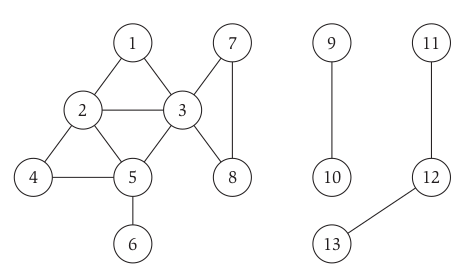
\includegraphics[width=0.5\textwidth]{Imagenes-Seccion3/fig32.png}
\caption{En este grafo, el nodo 1 tiene caminos a los nodos 2 a 8, pero no a los nodos 9 a 13}
\label{fig32}
\end{figure}

    Para grafos muy pequeños, esta pregunta puede ser respondida fácilmente, a partir de una inspección visual. Sin embargo, para grafos de mayores dimensiones, puede dar un poco de trabajo encontrar ese camino. En efecto el problema de la "conexión $s-t$" puede también ser llamado el "Problema de Resolución del Laberinto". Si imaginamos $G$ como un laberinto, con una habitación correspondiente a cada nodo, y un pasillo correspondiente a cada arista que une cada nodo (habitación), entonces el problema es empezar en una habitación $s$ y encontrar el camino para llegar a otra habitación $t$. ¿Qué tan eficiente puede ser un algoritmo diseñado para esta tarea? \\

    En esta sección describimos dos algoritmos naturales para este problema en un alto nivel: búsqueda de primer nivel (BFS por sus siglas en ingles "Breadth-First Search") y búsqueda en profundidad (DFS por sus siglas en ingles "Depth-First Search). En la siguiente sección discutiremos como implementar cada uno de estos eficientemente, construyendo una estructura de datos para representar grafos como la entrada a un algoritmo.
    
\subsubsection*{Búsqueda de primer nivel}  
Quizás el algoritmo más simple para determinar la conexión $s-t$ es BFS, en el cual exploramos hacia afuera partiendo desde $s$ en todas las direcciones posibles, añadiendo nodos a una "capa" a la vez. De esta forma empezamos con $s$ e incluimos todos los nodos que son alcanzados por una arista a $s$ (esta es la primera capa de búsqueda). Entonces incluimos todos los nodos adicionales que son alcanzados por una arista a cualquier nodo de la primera capa (esta es la segunda capa). Continuamos de esta forma hasta no encontrar más nodos nuevos. \\\\
En el ejemplo de la figura 7, empezando con el nodo 1 como $s$, la primera capa de búsqueda consiste en los nodos 2 y 3, la segunda capa consiste en los nodos 4, 5, 7 y 8, y la tercera capa consiste únicamente del nodo 6. En este punto la búsqueda termina, puesto que no hay más nodos que puedan ser agregados (en particular notar que los nodos 9 a 13 nunca son alcanzados por la búsqueda).
\\

Como este ejemplo refuerza, hay una interpretación física natural para este algoritmo. Esencialmente, comenzamos en $s$ e "inundamos" el grafo con una ola que crece para visitar todos los nodos que puede alcanzar. La capa que contiene un nodo representa el punto en el tiempo en el cual dicho nodo es alcanzado.
\\\\
Podemos definir las capas $L_1,L_2,L_3...$ construidas por el algoritmo BFS más precisamente como sigue:
	\begin{enumerate}
      \item La capa $L_1$ consiste de todos los nodos que son vecinos de $s$ (por razones de notación, en ocasiones usaremos la capa $L_0$ para denotar el conjunto formado únicamente por $s$).
      \item Asumiendo que hemos definido las capas $L_1,...L_j$, entonces la capa $L_{j+1}$ consiste de todos los nodos que no pertenecen a una capa anterior y que tienen una arista a un nodo en la capa $L_j$.
    \end{enumerate}
Volviendo a llamar a nuestra definición de distancia entre dos vértices como el mínimo número de aristas en un camino que lo une, vemos que la capa $L_1$ es el conjunto de todos los nodos a distancia 1 de $s$, y más genérico, la capa $L_j$ es el conjunto de todos los nodos a distancia exactamente $j$ desde s. Un nodo falta en aparecer en cualquiera de las capas si y solo si no hay un camino hacia el. Así, BFS no está solamente determinando los nodos a los que $s$ puede llegar, sino que también está computando los caminos más cortos a él. Resumimos esto en la siguiente proposición.
\\ \\
 \colorbox{mygray}{\parbox{15cm}{
	\textbf{(3.3):} Para cada $j \geq 1$ , la capa $L_j$, producida por BFS consiste de todos los nodos a una distancia exactamente $j$ desde $s$. Hay un camino desde $s$ hasta $t$ si y solo si $t$ aparece en alguna capa.

  }}\\
  \\
  Otra propiedad de BFS es que produce, de forma muy natural, un árbol T con raíz $s$ en el conjunto de nodos alcanzables desde $s$. Específicamente, para cada nodo $v$ (distinto de $s$), consideremos el momento cuando $v$ es descubierto por primera vez por el algoritmo BFS; esto ocurre cuando algún nodo $u$ en la capa $L_j$ está siendo examinado, y encontramos que tiene una arista a un vértice anteriormente no visto  $v$. En este momento, agregamos la arista $(u,v)$ al árbol $T$ $u$ se hace padre de $v$, representando el caso de que $u$ es responsable de completar el camino a $v$. Llamamos a ese árbol $T$ como $breadth-first search tree$.\\
  
La figura  \ref{fig33} representa la construcción del árbol con raíz en el nodo 1 para el grafo de la figura  \ref{fig32}. Las aristas continuas son las aristas de $T$; las aristas discontinuas son las aristas de $G$ que no pertenecen a $T$. La ejecución de BFS que produce este árbol puede ser descrito de la siguiente forma:

   \begin{enumerate}
   		\item Empezando desde el nodo 1, la capa $L_1$ consiste de los nodos (2,3).
        \item La capa $L_2$, crece considerando los nodos de la capa $L_1$ en orden (es decir, primero 2, luego 3). Así descubrimos los nodos 4 y 5 tan pronto como miramos al 2, así que 2 se convierte en su padre. Cuando consideramos el nodo 2, también descubrimos una arista a 3, pero no es agregado al árbol BFS, ya que ya sabemos sobre este nodo.\\
        
	Primero descubrimos los nodos 7 y 8, cuando miramos al nodo 3. Por otro lado, la arista desde 3 a 5 es otra arista de $G$ que no termina en el árbol BFS, porque al mismo tiempo que miramos esta arista desde el nodo 3, sabemos sobre el nodo 5.
    \item Ahora consideramos los nodos de la capa $L_2$, en orden, pero el único nuevo nodo descubierto cuando miramos a través de $L_2$ es el nodo 6, el cual es agregado a la capa $L_3$. Notar que las aristas (4,5) y (7,8) no son agregados al árbol BFS, ya que no resultan en el descubrimiento de nuevos nodos.
    \item Ningún nuevo nodo es descubierto cuando el nodo 6 es examinado, así que ninguno es puesto en la capa $L_4$, y el algoritmo termina. El árbol completo está representado en la figura 7(c).
   \end{enumerate}
   
\begin{figure}[h]
\centering
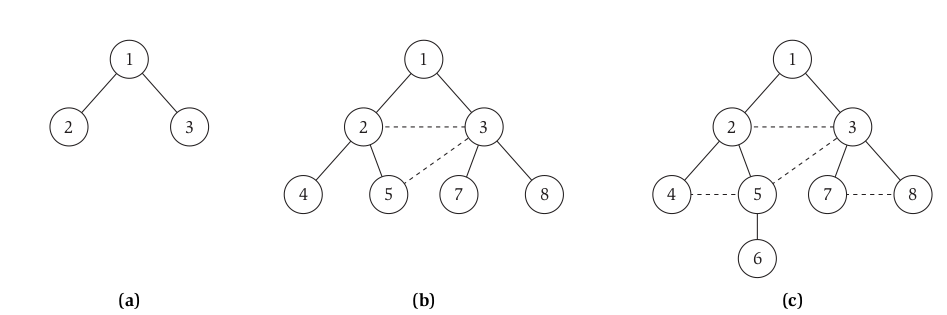
\includegraphics[width=0.7\textwidth]{Imagenes-Seccion3/fig7.png}
\caption{La construcción del árbol BFS para el grafo de la figura 6. Con (a), (b) y (c) representando la sucesión de capas que son agregadas. Las aristas continuas son aristas de $T$; las aristas discontinuas esta en la componente conectada de $G$ conteniendo al nodo 1, pero no perteneciendo a $T$}
 \label{fig33}
\end{figure}

Nos damos cuenta que a medida que corremos BFS en este grafo, las aristas del árbol que se obtiene no conectan nodos en la misma capa pero sí en capas adyacentes. \\

 \colorbox{mygray}{\parbox{15cm}{
	\textbf{(3.4):} Tomemos $T$ un árbol BFS, tomemos $x$ e  $y$ nodos en $T$, perteneciendo a las capas $L_i$ y $L_j$ respectivamente, y tomemos $(x,y)$ una arista de $G$. Entonces $i$ y $j$ difieren a lo sumo 1.}}\\\\
  
\textbf{Demostración:} Supongamos por absurdo que $i$ y $j$ difieren por más de 1; en particular supongamos que $i < j - 1$. Ahora consideremos el punto en el algoritmo BFS cuando las aristas incidentes a $x$ son examinadas. Sabiendo que $x$ pertenece a la capa $L_i$, los únicos nodos descubiertos desde $x$ pertenecen a la capa $L_{i+1}$ o anteriores. $ \blacksquare $ 

\begin{figure}[h]
\centering
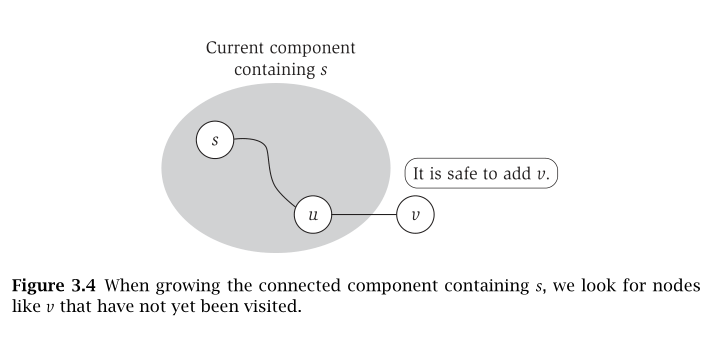
\includegraphics[scale=1]{Imagenes-Seccion3/fig3_3.PNG}
\caption{}
\end{figure}

\subsubsection*{Explorando una componente conexa}  

El conjunto de nodos descubiertos por el algoritmo BFS es precisamente los alcanzables desde el nodo de inicio $s$. Nos referiremos a este conjunto $R$ como la componente conexa de $G$ que contiene a $s$; y una vez que sabemos que dicha componente lo contiene, simplemente podemos verificar si $t$ pertenece a él para responder la pregunta de conexión $s-t$. \\

Ahora, si uno lo piensa, está claro que BFS es solo una manera posible de
producir esta componente. En un nivel más general, podemos construir la componente
$R$ "explorando" $G$ en cualquier orden, comenzando desde $s$. Para comenzar, definimos $R = {s}$. Entonces, en cualquier punto en el tiempo, si encontramos una arista $(u, v)$ donde $u  \in  R$ y \(v \notin  R\), puede agregar $v$ a $R$. De hecho, si hay un camino $P$ de $s$ a $u$, entonces hay un camino de $s$ a $v$ obtenido al seguir primero a $P$ y luego seguir la arista $(u, v)$. \\

La Figura 3.4 ilustra este paso básico en el crecimiento de la componente $R$.
Supongamos que seguimos creciendo el conjunto $R$ hasta que no hayan más aristas
que salen de $R$; en otras palabras, ejecutamos el siguiente algoritmo:

\begin{lstlisting}
R consistira en los nodos de s que tiene un camino 
Inicialmente R = {s}
Mientras hay una arista (u, v) donde u en R y v no esta en R
   agregar v a R
Fin del Mientras
\end{lstlisting}

Aquí está la propiedad clave de este algoritmo:\\


 \colorbox{mygray}{\parbox{15cm}{
	\textbf{(3.5):} El conjunto $R$ producido al final del algoritmo es precisamente la componente conexa de $G$ que contiene a $s$.}}\\\\

\textbf{Demostración:} ya hemos argumentado que para cualquier nodo $v  \in  R$, hay una ruta desde $s$ a $v$.\\

Ahora, considere un nodo $w \not{\epsilon} R$, y suponga a modo de contradicción, que
hay un camino $s-w$ $P$ en $G$. Dado que $s  \in  R$ pero $w \not{\epsilon} R$, debe haber un primer nodo $v$ en $P$ que no pertenece a $R$; y este nodo $v$ no es igual a $s$. Por lo tanto, hay un nodo $u$ inmediatamente anterior $v$ en $P$, entonces $(u, v)$ es una arista. Por otra parte, desde $v$ es el primer nodo en $P$ que no pertenece a $R$, debemos tener $u  \in  R$. Sigue que $(u, v)$ es una arista donde $u  \in  R$ y $v \not{\epsilon} R$; esto contradice la regla de parar el algoritmo. $ \blacksquare $ \\

Para cualquier nodo $t$ en la componente $R$, observe que es fácil recuperar el
camino real de $s$ a $t$ a lo largo de las líneas del argumento anterior: simplemente registramos, para cada nodo $v$, la arista $(u, v)$ que se consideró en la iteración en la que $v$ se agregó a $R$. Luego, al trazar estas aristas hacia atrás desde $t$, procedemos a través de una secuencia de nodos que se agregaron en iteraciones anteriores, eventualmente alcanzando $s$; esto define un camino $s-t$. \\

Para concluir, notamos que el algoritmo general que hemos definido para
crecer $R$ no está especificado, entonces, ¿cómo decidimos qué arista considerar a continuación? El algoritmo BFS surge, en particular, como una forma particular de ordenar los nodos que visitamos, en capas sucesivas, en función de su distancia desde $s$. Pero hay otras formás naturales de hacer crecer la componente, varias de las cuales conducen a algoritmos eficientes para el problema de conexión mientras se produce la búsqueda de patrones con diferentes estructuras. Ahora vamos a discutir una diferencia de estos algoritmos, búsqueda en profundidad, y desarrollar algunas de sus propiedades básicas.

\subsubsection*{Búsqueda de primera profundidad (DFS Depth-First Search) }  

Otro método natural para encontrar los nodos accesibles desde $s$ es el enfoque que
podría tomar si el grafo $G$ fuera realmente un laberinto de habitaciones interconectadas y usted estaba caminando en eso. Empezaría desde $s$ y probaría la primera ventaja de ello, a un nodo $v$. Luego seguiría la primera arista que sale de $v$, y continuará de esta manera hasta llegar a un "callejón sin salida", un nodo para el que ya exploró a todos sus vecinos. Luego retrocederías hasta llegar a un nodo con un vecino inexplorado, y reanudar desde allí. Llamamos a este algoritmo depth-first search (DFS), ya que explora $G$ yendo tan profundamente como sea posible y solo retirarse cuando sea necesario. \\

DFS es una implementación particular de BFS que ya fue descrito anteriormente. Se describe más fácilmente recursivamente: podemos invocar DFS desde cualquier punto de partida, pero mantener el conocimiento global de los nodos que ya han sido explorados. \\


\begin{lstlisting}
DFS(u):
  Marcar u como "Explorado" y agregar u a R
  Para cada arista  (u, v) incidente a u
     SI v  no ha sido marcado como "Explorado" entonces
        Invocamos recursivamente DFS(v)
     Fin del SI
Fin de para cada
\end{lstlisting}

Para aplicar esto a la conexión $s-t$, simplemente declaramos que todos los nodos inicialmente no son explorados, e invocamos DFS (s).\\

Hay algunas similitudes fundamentales y algunas diferencias fundamentales entre DFS y BFS. Las similitudes se basan en el hecho de que ambos construyen la componente conexa que contiene $s$, y veremos en la siguiente sección que alcanzan niveles de eficiencia cualitativamente similares.\\

Mientras que DFS finalmente visita exactamente el mismo conjunto de nodos que BFS, típicamente lo hace en un orden muy diferente; explora su camino por largos caminos, potencialmente muy alejados de $s$, en vez de retroceder para probar nodos inexplorados más cercanos. Nosotros podemos ver un reflejo de esta diferencia en el hecho de que, al igual que BFS, el algoritmo DFS produce un árbol $T$ con raíz natural $s$, pero el árbol generalmente tienen una estructura muy diferente. El algoritmo se decodifica así: hacemos a $s$ la raíz del árbol $T$, y luego hacemos el padre de $v$ cuando es responsable del descubrimiento de $v$. Es decir, cada vez que se invoca DFS ($v$) directamente durante la llamada a DFS ($u$), agregamos la arista $(u, v)$ a $T$. El árbol resultante se denomina árbol de búsqueda en profundidad de la componente $R$.\\

La figura \ref{Fig35} muestra la construcción de un árbol DFS con raíz en el nodo 1 para el grafo de la Figura \ref{fig32}. Las aristas no punteadas son las aristas de $T$  que están en $G$ y las punteadas son las aristas de $G$ que no están en $T$. La ejecución de DFS comienza mediante la construcción de un camino en los nodos 1, 2, 3, 5, 4. La ejecución llega a un callejón sin salida en 4, ya que no hay nuevos nodos que encontrar, por lo que "retrocede" a 5, encuentra el nodo 6, realiza una copia de seguridad de nuevo a 3, y encuentra los nodos 7 y 8. En este punto no hay nuevos nodos para encontrar en la componente conexa, por lo que todas las llamadas DFS recursivas pendientes terminan, una por una, y la ejecución llega a su fin. Se representa el árbol DFS completo en la figura \ref{Fig35}(g).\\

Este ejemplo sugiere la forma característica en que los árboles DFS se ven
diferente de los árboles BFS. En lugar de tener caminos de raíz a hoja que son tan cortos como sea posible, tienden a ser bastante estrechos y profundos. Sin embargo, como en el caso de BFS, podemos decir algo bastante fuerte sobre la forma en la que
las aristas de $G$ deben estar dispuestas en relación con las aristas de un árbol DFS $T$: como en el de la figura, las aristas que no están en el árbol solo pueden conectar antepasados de $T$ con descendientes.

\begin{figure}[h]
\centering
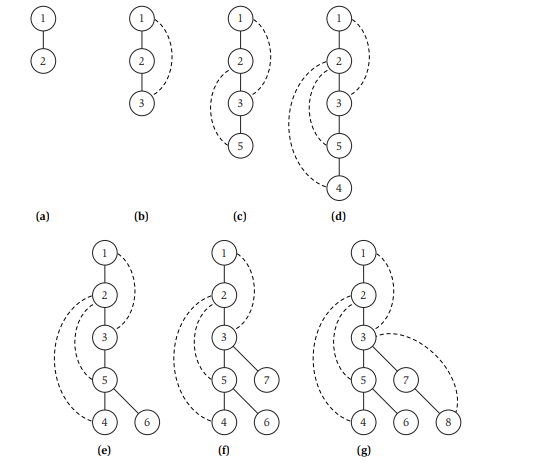
\includegraphics[scale=1]{Imagenes-Seccion3/fig3_5.PNG}
\caption{La construcción de un árbol T de búsqueda de primera profundidad para el grafo de la figura 6 con los pasos de (a) hasta (g), que representan los nodos a medida que se van descubriendo. Las aristas no punteadas son las aristas de T mientras que las punteadas son aristas de G que no pertenecen a T.}
\label{Fig35}
\end{figure}


Para establecer esto, primero observamos la siguiente propiedad del árbol generado por el algoritmo DFS:\\

 \textbf{(3.6)} Para una llamada recursiva dada DFS ($u$), todos los nodos que están marcados como "Explorado" entre la invocación y el final de esta llamada recursiva son descendientes de $u$ en $T$.\\

Usando (3.6) probemos:\\

 \colorbox{mygray}{\parbox{15cm}{
	\textbf{(3.7):} Si $T$ es un árbol de búsqueda en profundidad en el que $x$ e $y$ sean nodos en $T$ y si $(x, y)$ es una arista de $G$ que no es una arista de $T$. Entonces $x$ o $y$ es un antepasado del otro.}}\\\\
    
\textbf{Demostración:} Supongamos que $(x, y)$ es una arista de $G$ que no es una arista de $T$, y supongamos sin pérdida de generalidad que $x$ es alcanzado primero por el algoritmo DFS. Cuando la arista $(x, y)$ se examina durante la ejecución de DFS ($x$), no se agrega a $T$ porque $y$ está marcado como "Explorado". Como $y$ no estaba marcado como "Explorado" cuando DFS ($x$) se invocó por primera vez, resulta que $y$ es un nodo que se descubrió entre invocación y finalización de la llamada recursiva DFS ($x$). De (3.6) se desprende que $y$ es un descendiente de $x$. $ \blacksquare $

\subsubsection*{El conjunto de todas las componentes conexas} 

Hasta ahora hemos estado hablando sobre la componente conexa que contiene a un
nodo particular $s$. Pero hay una componente conexa asociado con cada
nodo en el grafo. ¿Cuál es la relación entre estas componentes?\\

De hecho, esta relación está muy estructurada y se expresa en la siguiente proposición.\\

 \colorbox{mygray}{\parbox{15cm}{
	\textbf{(3.8):} Para dos nodos $s$ y $t$ en un grafo, sus componentes conexas son
idénticas o disjuntas.}}\\\\

Esta es una afirmación que es muy clara intuitivamente, si uno mira un grafo como
el ejemplo en la figura \ref{fig32}. El grafo está dividido en varias piezas sin
aristas entre ellas; la pieza más grande es la componente conexa de los nodos
1 a 8, la pieza mediana es la componente conexa de los nodos 11, 12 y 13, y la pieza más pequeña es la componente conexa de los nodos 9 y 10. Para demostrar la afirmación en general, solo tenemos que mostrar cómo definir estas "piezas" precisamente para un grafo arbitrario.\\

\textbf{Demostración:} considere dos nodos $s$ y $t$ en un grafo $G$ con la propiedad que hay un camino entre $s$ y $t$. Afirmamos que las componentes conexas que contienen a $s$ y a $t$ son el mismo conjunto. De hecho, para cualquier nodo $v$ que esté en la componente de $s$ también debe ser accesible desde $t$ por un camino: podemos simplemente caminar de $t$ a $s$, y luego de $s$ a $v$. El mismo razonamiento funciona con los roles de $s$ y $t$ invertidos, por lo que un nodo está en la componente de uno si y solo si está en la componente del otro. Por otro lado, si no hay un camino entre $s$ y $t$, entonces no puede haber un nodo $v$ que está en la componente conexa de cada uno. Pues, si hubiera tal nodo $v$, entonces podríamos caminar de $s$ a $v$ y luego a $t$, construyendo un camino entre $s$ y $t$. Por lo tanto, si no hay un camino entre $s$ y $t$, entonces las componentes conexas son disjuntas. $ \blacksquare $ \\

Esta prueba sugiere un algoritmo natural para producir todas las componentes
conexas de un grafo, haciéndolos crecer de a una componente a la vez. Empezamos
con un nodo arbitrario $s$ y usamos BFS (o DFS) para generar su componente conexa. Luego encontramos un nodo $v$ (si hay alguno) que no fue visitado por la búsqueda
desde $s$ e iteramos usando BFS comenzando desde $v$, para generar su componente la que por (3.8) será disjunta de la componente de $s$. Continuamos de esta manera hasta que se hayan visitado todos los nodos.

\subsection{Implementación del recorrido de un grafo usando colas y pilas}

Hasta aquí hemos estado discutiendo primitivas básicas de algoritmos para trabajar con
grafos sin mencionar ningún detalle de implementación. Aquí discutiremos cómo
usar listas y arrays para representar grafos, y discutiremos las concesiones
entre las diferentes representaciones. Luego usaremos estas estructuras de datos para
implementar los algoritmos de recorrido de grafos \textit{breadth-first search} (BFS) y \textit{depth-first search} (DFS) de manera eficiente. Veremos que BFS y DFS difieren esencialmente solo en eso: uno usa una \textit{cola} y el otro usa una \textit{pila}. Dos estructuras de datos que describiremos más adelante en esta sección.

\subsubsection*{Representando Grafos} 
\paragraph{}
Hay dos formás básicas de representar grafos: mediante una matriz de adyacencia y por una representación de lista de adyacencia. A lo largo del libro usaremos el representación de la lista de adyacencia. Comenzaremos, sin embargo, revisando estas dos representaciones y discutiendo las concesiones entre ellas.

Un grafo \(G = (V, E)\) tiene dos parámetros de entrada naturales, el número de nodos \(|V|\), y el número de aristas \(|E|\). Utilizaremos \( n = |V|\) y \(m = |E|\) para denotar estos, respectivamente. Los tiempos de ejecución se darán en términos de estos dos parámetros. Como de costumbre, buscaremos tiempos de ejecución polinomiales, y los polinomios de menor grado son mejores. Sin embargo, con dos parámetros en el tiempo de ejecución, la comparación no siempre es tan clara. ¿Es \(O(m^{2})\) u \(O(n^{3})\) un mejor tiempo de ejecución? Esto depende de la relación entre $n$ y $m$. Con a lo sumo una arista entre cualquier par de nodos, el número de aristas $m$ puede ser como máximo \(\binom{n}{2} ≤ n^{2}\). Por otro lado, en muchas aplicaciones los grafos de interés son conexos, y según \textit{(3.1)}, los grafos conexos deben tener al menos \(\textit{m ≥ n }- 1\) aristas. Pero estas comparaciones no siempre nos dicen cuál de los dos tiempos de ejecución (como \(m^{2}\) y \(n^{3}\)) es mejor, por lo que tenderemos a mantener los tiempos de ejecución en términos de estos dos parámetros. En esta sección pretendemos implementar los algoritmos básicos de búsqueda de grafos en el tiempo \(O(m+n)\). Nos referiremos a esto como \textit{tiempo lineal}, ya que toma \(O(m+n)\) tiempo simplemente para leer la entrada. Tenga en cuenta que cuando trabajamos con grafos conexos, un tiempo de ejecución de \(O(m+n)\) es el mismo que \(O(m)\), ya que \( m ≥ n - 1.\)\\ 

Considere un grafo $G = (V, E)$ con \textit{n} nodos, y suponga que el conjunto de nodos es $V = \{1,. . . , n\}$. La forma más sencilla de representar un grafo es mediante una matriz A de adyacencia, que es una matriz \(n × n\) donde A[$u,v$] es igual a 1 si el grafo contiene la arista \textit{($u$,$v$)} y 0 en caso contrario. Si el grafo no está dirigido, la matriz A es simétrica, con A[$u,v$] = A[$v,u$] para todos los nodos $u$, $v  \in  V$. La representación de la matriz de adyacencia nos permite verificar en \(O(1)\) si una arista dada ($u$, $v$) está presente en el grafo. Sin embargo, la representación tiene dos desventajas básicas.

\begin{itemize}
\item La representación toma \(\Theta (n^{2})\) espacio. Cuando el grafo tiene muchos menos aristas que \(n^{2}\), se pueden encontrar representaciones más compactas.
\item Muchos algoritmos de grafos necesitan examinar todas las aristas incidentes en un nodo dado $v$. En la representación de la matriz de adyacencia, hacer esto implica considerar todos los otros nodos $w$, y verificar la entrada de matriz A [$v$, $w$] para ver si la arista ($v, w$) está presente, y esto lleva \(\Theta (n)\) tiempo. En el peor de los casos, $v$ puede tener \(\Theta (n)\) aristas incidentes, en cuyo caso el control de todas estas aristas tomará tiempo \(\Theta (n)\) independientemente de la representación. Pero muchos grafos en la práctica tiene significativamente menos aristas incidentes en la mayoría de los nodos, por lo que sería bueno poder encontrar todas estas aristas de incidente de manera más eficiente.
\end{itemize}
\paragraph{}
La representación de los grafos utilizados en todo el libro es la lista de adyacencia, que funciona mejor para grafos dispersos-es decir, aquellos con muchos menos que \(n^{2}\) aristas. En la representación de la \textit{lista de adyacencia} hay un registro para cada nodo $v$, que contiene una lista de los nodos a los que $v$ tiene aristas. Para ser precisos, tenemos un array Adj, donde Adj[$v$] es un registro que contiene una lista de todos los nodos adyacentes al nodo v. Para un grafo no dirigido $G = (V, E)$, cada arista $e =(v, w)   \in  E$ ocurre en dos listas de adyacencia: el nodo $w$ aparece en la lista para el nodo $v$, y el nodo $v$ aparece en la lista para el nodo $w$.\\

Comparemos la matriz de adyacencia y las representaciones de la lista de adyacencia. Primero considere el espacio requerido por la representación. Una matriz de adyacencia requiere \(O(n^{2})\) espacio, ya que utiliza una matriz $n × n$. Por el contrario, afirmamos que la representación de la lista de adyacencia requiere solo \(O(m + n)\) espacio. Aquí está el por qué. Primero, necesitamos una serie de punteros de longitud $n$ para configurar las listas en Adj, y luego necesitamos espacio para todas las listas. Ahora, las longitudes de estas listas pueden diferir de nodo a nodo, pero argumentamos en el párrafo anterior que en general, cada arista \(e = (v, w)\) aparece en exactamente dos de las listas: la de $v$ y la de $w$ . Por lo tanto, la longitud total de todas las listas es \(2m = O(m)\).
\\Otra forma (esencialmente equivalente) de justificar este límite es la siguiente. Definimos el \textit{grado} \(n_{v}\) de un nodo $v$ como el número de aristas de incidente que tiene. La longitud de la lista en Adj[$v$] es \(n_{v}\), por lo que la longitud total de todos los nodos es \(O( \sum_{v\epsilon V} {n_{v}})\) . Ahora, la suma de los grados en un grafo es una cantidad que a menudo aparece en el análisis de los algoritmos de grafos, por lo que es útil determinar cuál es esta suma.
\paragraph{}
\textbf{(3.9)} \(\sum_{v\epsilon V} {n_{v}} = 2m\)\\

\textbf{Demostración:} Cada arista \(e = (v, w)\) contribuye exactamente dos veces a esta suma: una vez en la cantidad \(n_{v}\) y una vez en la cantidad \(n_{w}\). Dado que la suma es el total de las contribuciones de cada arista, es \textit{2m}. $ \blacksquare $ \\

Resumimos la comparación entre matrices de adyacencia y listas de adyacencia de la siguiente manera.
\paragraph{}
\colorbox{mygray}{\parbox{15cm}{
	\textbf{(3.10):} La representación de la matriz de adyacencia de un grafo requiere \(O(n^{2})\) espacio, mientras que la representación de la lista de adyacencia requiere solo \(O(m+n)\) espacio}}\\\\
    
    Como ya hemos discutido que \(m ≤ n^{2}\), el limite \(O(m+n)\)  nunca es peor que \(O(n^{2})\); y es mucho mejor cuando el grafo subyacente es \textit{disperso}, con m mucho más pequeño que \(n^{2}\).
    
    Ahora consideramos la facilidad de acceso a la información almacenada en estas dos representaciones diferentes. Recuerde que en una matriz de adyacencia podemos verificar en tiempo \(O(1)\) si una arista particular ($u, v$) está presente en el grafo. En la representación de la lista de adyacencia, esto puede llevar un tiempo proporcional al grado \(O(n_{v})\): tenemos que seguir los punteros en la lista de adyacencia para ver si el nodo $v$ aparece en la lista. Por otro lado, si el algoritmo está actualmente mirando un nodo u, puede leer la lista de vecinos en tiempo constante por vecino.
   
   En vista de esto, la lista de adyacencia es una representación natural para explorar grafos. Si el algoritmo está actualmente mirando un nodo $u$, puede leer esta lista de vecinos en tiempo constante por vecino; pasar a un vecino $v$ una vez que lo encuentra en esta lista en tiempo constante; y luego estar listo para leer la lista asociada con el nodo $v$. La representación de la lista corresponde a una noción física de "explorar" el grafo, en la que aprende los vecinos de un nodo $u$ una vez que llega a $u$, y puede leerlos en tiempo constante por vecino

\subsubsection*{Colas y Pilas} 
\paragraph{}
Muchos algoritmos tienen un paso interno en el que necesitan procesar un conjunto de elementos, como el conjunto de todas las aristas adyacentes a un nodo en un grafo, el conjunto de nodos visitados en BFS y DFS, o el conjunto de todos los hombres libres en el Algoritmo de Emparejamiento Estable (Stable Matching Algorithm). Para este propósito, es natural mantener el conjunto de elementos a ser considerado en una lista vinculada, como lo hemos hecho para mantener el conjunto de hombres libres en el Algoritmo de Emparejamiento Estable.\\

Una cuestión importante que surge es el orden en el que se deben considerar los elementos en dicha lista. En el Algoritmo de Emparejamiento Estable, el orden en el que consideramos los hombres libres no afectó el resultado, aunque esto requirió una prueba bastante sutil para verificar. En muchos otros algoritmos, como DFS y BFS, el orden en que se consideran los elementos es crucial.\\

Dos de las opciones más simples y naturales son mantener un conjunto de elementos como una cola o una pila. Una cola es un conjunto del que extraemos elementos en orden tal que el primero en entrar es el primero en salir (FIFO, \textit{first-in, first-out}): seleccionamos elementos en el mismo orden en que fueron agregados. Una pila es un conjunto del cual extraemos elementos en orden tal que el último en entrar es el primero en salir (LIFO,\textit{last-in, first-out}): cada vez que seleccionamos un elemento, elegimos
el que se agregó más recientemente. Tanto las colas como las pilas se pueden implementar fácilmente a través de una lista doblemente encadenada. En ambos casos, siempre seleccionamos el primer elemento en nuestra lista; la diferencia está en donde insertamos un nuevo elemento. En una cola se agrega un nuevo elemento al final de la lista como último elemento, mientras que en una pila se coloca un nuevo elemento en la primera posición de la lista. Recuerde que una lista doblemente encadenada tiene punteros \textit{Primero} y \textit{Último} explícitos al principio y al final, respectivamente, de modo que cada una de estas inserciones se puede hacer en tiempo constante.\\\

A continuación discutiremos cómo implementar los algoritmos de búsqueda de la sección anterior en tiempo lineal. Veremos que se puede pensar que BFS utiliza una cola para seleccionar qué nodo considerar a continuación, mientras que DFS está utilizando efectivamente una pila.\\
    
\subsubsection*{Implementar BFS} 
\paragraph{} 
La estructura de datos de la lista de adyacencia es ideal para implementar BFS. El algoritmo examina las aristas dejando un nodo dado uno por uno. Cuando estamos escaneando las aristas dejadas y llegando a una arista ($u, v$), necesitamos saber si el nodo $v$ ha sido descubierto previamente por la búsqueda. Para simplificar esto, mantenemos una matriz \textit{Discovered} de longitud $n$ y establecemos  \textit{Discovered}[$v$] = \textit{true} tan pronto como nuestra búsqueda ve primero $v$. El algoritmo, como se describe en la sección anterior, construye capas de nodos \(L_{1}, L_{2},. . . \), donde \(L_{i}\) es el conjunto de nodos a la distancia $i$ de la fuente $s$. Para mantener los nodos en una capa \(L_{i}\), tenemos una lista L[$i$] para cada $i = 0, 1, 2,. . . .$

\begin{lstlisting}
BFS(s):
Establecer Descubierto[s] = verdadero y Descubierto[v] = falso para todos los demas v
Inicializar L[0] para que este formado unicamente por el elemento s
Establecer el contador de capas i = 0
Establecer el arbol BFS actual T = null
MIENTRAS  L[i] no esta vacio
	Inicializar una lista vacia L[i + 1]
	PARA cada cada nodo u en L[i]
		Considere cada arista (u, v) que le inside a u
		SI Descubierto[v] = falso entonces
			Establecer Descubierto[v] = verdadero
			Agregar la arista (u, v) al arbol T
            Agregar v a la lista L[i + 1]
		fin del SI
	fin del PARA
Contador de capas +1
Fin del MIENTRAS
\end{lstlisting}

En esta implementación, no importa si manejamos cada lista L[$i$] como una cola o una pila, ya que el algoritmo puede considerar los nodos en una capa \(L_{i}\) en cualquier orden.
\paragraph{}

\colorbox{mygray}{\parbox{15cm}{
	\textbf{(3.11):} La implementación anterior del algoritmo BFS se ejecuta en el tiempo \(O(m+n)\) (es decir, lineal en el tamaño de entrada), si el grafo está dado por la representación de la lista de adyacencia.}}\\
    
\textbf{Demostración:} Como primer paso, es fácil acotar el tiempo de ejecución del algoritmo con \(O(n^{2})\) (un límite más débil que nuestro \(O(m+n)\)). Para ver esto, tenga en cuenta que hay como mucho $n$ listas L[$i$] que necesitamos establecer, por lo que esto toma \(O(n)\) tiempo. Ahora tenemos que considerar los nodos $u$ en estas listas. Cada nodo ocurre en a lo sumo una lista, por lo que el bucle For se ejecuta como máximo $n$ veces sobre todas las iteraciones del bucle While. Cuando consideramos un nodo u, necesitamos mirar todas las aristas ($u, v$) incidentes para $u$. Puede haber como máximo n tales aristas, y pasamos \(O(1)\) tiempo considerando cada arista. Por lo tanto, el tiempo total empleado en una iteración del ciclo For es como máximo \(O(n)\). Por lo tanto, hemos llegado a la conclusión de que hay como mucho $n$ iteraciones del bucle For, y que cada iteración tarda como máximo \(O(n)\) tiempo, por lo que el tiempo total es como máximo \(O(n^{2})\).
\paragraph{}
Para obtener la cota \(O(m + n)\), debemos observar que el ciclo For para procesar un nodo u puede tomar menos que \(O(n)\) tiempo si u tiene solo unos pocos vecinos. Como anteriormente, sea \(n_{u}\)  el grado de nodo u, el número de aristas incidentes a $u$. Ahora, el tiempo pasado en el bucle For considerando las aristas incidentes al nodo $u$ es \(O(n_{u})\), por lo que el total sobre todos los nodos es \(O(\sum_{u\epsilon V} {n_{u}})\). Recuerde \textit{(3.9)} que \(\sum_{u\epsilon V} {n_{u}} = 2m\) y por lo tanto el tiempo total dedicado considerando las aristas sobre el algoritmo completo es \(O(m)\). Necesitamos \(O(n)\) tiempo adicional para configurar listas y administrar la matriz\textit{ Discovered}. Entonces, el tiempo total es \(O(m+n)\) como se afirmó. $ \blacksquare $ \\

Describimos el algoritmo usando hasta $n$ listas separadas L[$i$] para cada capa \(L_{i}\). En lugar de todas estas listas distintas, podemos implementar el algoritmo usando una sola lista L que mantenemos como una cola. De esta forma, el algoritmo procesa los nodos en el orden en que se "descubren" por primera vez: cada vez que se "descubre" un nodo,
se agrega al final de la cola y el algoritmo siempre procesa las aristas del nodo que actualmente está primero en la cola.
Si mantenemos los nodos "descubiertos" en este orden, todos los nodos en la capa \(L_{i}\) aparecerán en la cola delante de todos los nodos en la capa \(L_{i+1}\), for \(i = 0, 1, 2. . .\). Por lo tanto, todos los nodos en la capa \(L_{i}\) se considerarán en una secuencia contigua, seguidos por todos los nodos en la capa \(L_{i+1}\), y así sucesivamente. Por lo tanto, esta implementación en términos de una cola única producirá el mismo resultado que la implementación de BFS anterior.

\subsubsection*{Implementar DFS} 
\paragraph{}
Ahora consideramos el algoritmo de DFS. En la sección anterior
presentamos DFS como un procedimiento recursivo, que es una forma natural de especificarlo. Sin embargo, también se puede ver como casi idéntico a BFS, con la diferencia que mantiene los nodos procesados en una pila, en lugar de en una cola. Esencialmente, la estructura recursiva de DFS se puede ver como nodos de empuje en una pila para su posterior procesamiento, mientras avanza a nodos más recientemente "descubiertos". Ahora mostraremos cómo implementar DFS al mantener esta pila de nodos para ser procesados explícitamente.\\

Tanto en BFS como en DFS, hay una distinción entre el acto de "descubrir"
un nodo $v$ (la primera vez que se ve, cuando el algoritmo encuentra una arista a $v$) y al acto de explorar un nodo $v$, cuando todos las aristas incidentes a $v$ son escaneadas, lo que resulta en el descubrimiento potencial de otros nodos. La diferencia entre BFS y DFS radica en la forma en que el descubrimiento y la exploración son intercalados.\\

En BFS, una vez que comenzamos a explorar un nodo $u$ en la capa \(L_{i}\), agregamos todos sus vecinos recién descubiertos a la siguiente capa \(L_{i+1}\), y diferimos en realidad explorando estos vecinos hasta que llegamos al procesamiento de la capa \(L_{i+1}\). Por el contrario, DFS es más impulsivo: cuando explora un nodo $u$, escanea el vecinos de $u$ hasta que encuentre el primer nodo $v$ aún no explorado (si hay alguno), y luego inmediatamente cambia la atención a explorar $v$.\\

Para implementar la estrategia de exploración de DFS, primero agregamos todos los nodos adyacente a $u$ a nuestra lista de nodos a considerar, pero después de hacer esto, procede a explorar un nuevo vecino $v$ de $u$. A medida que exploramos $v$, a su vez, agregamos los vecinos de $v$ a la lista que estamos manteniendo, pero lo hacemos en orden de pila, para que estos vecinos sean explorados antes de que regresemos a explorar el otro vecinos de $u$. Solo volvemos a otros nodos adyacentes a $u$ cuando no quedan otros nodos.\\

Además, usamos una matriz \textit{Explored} análoga a la matriz \textit{Discovered} que utilizamos para BFS. La diferencia es que solo establecemos que \(Explored[v]= true\) cuando escaneamos las aristas incidentes de $v$ (cuando la búsqueda DFS está en $v$), mientras BFS establece \(Discovered[v]=true\) tan pronto como se descubre por primera vez $v$. La implementación es de la siguiente manera:
\paragraph{}
\begin{lstlisting}
DFS(s):
Inicializa S para que sea una pila con un elemento s
While que S no este vacio
	Toma un nodo u de S
	If Explored[u] = false then
		Establecer Explored[u] = true
		For cada arista (u, v) incidente para u
			Agregue v a la pila S
		Endfor
	Endif
Endwhile
\end{lstlisting}
\paragraph{}
Aun queda un ultimo detalle para mencionar. DFS no está especificado, ya que la lista de adyacencia de un nodo explorado se puede procesar en cualquier orden. Tenga en cuenta que el algoritmo anterior, porque empuja todos los nodos adyacentes a la pila antes de considerar cualquiera de ellos, de hecho procesa cada lista de adyacencia en el orden inverso en relación con la versión recursiva de DFS en la sección anterior.\\
\paragraph{}
\colorbox{mygray}{\parbox{15cm}{
	\textbf{(3.12):} El algoritmo anterior implementa DFS, en el sentido de que visita los nodos exactamente en el mismo orden que el procedimiento DFS recursivo en la sección anterior (excepto que cada lista de adyacencia se procesa en orden inverso).}}\\   
Si queremos que el algoritmo también encuentre el árbol DFS, necesitamos que cada nodo $u$ de la pila $S$ mantenga el nodo que "hizo" que $u$ se agregue a la pila. Esto se puede hacer fácilmente mediante el uso de un arrays \textit{parent} y la configuración \(parent[v] = u\) cuando agregamos el nodo $v$ a la pila debido a la arista ($u, v$). Cuando marcamos un nodo \(u \neq s\) como "Explorado", también podemos agregar la arista \((u, parent[u])\) al árbol $T$. Tenga en cuenta que un nodo $v$ puede estar en la pila $S$ varias veces, ya que puede ser adyacente a múltiples nodos $u$ que exploramos, y cada nodo agrega una copia de $v$ para la pila $S$. Sin embargo, solo usaremos una de estas copias para explorar el nodo $v$, la última copia que añadimos. Como resultado, basta con mantener un valor \(parent[v]\) para cada nodo $v$ simplemente sobrescribiendo el valor \(parent[v]\) cada vez que agregamos una nueva copia de $v$ a la pila $S$.\\
 
El paso principal en el algoritmo es agregar y eliminar nodos hacia y desde la pila $S$, que toma \(O(1)\) cada vez. Por lo tanto, para acotar el tiempo de ejecución, debemos acotar el número de estas operaciones. Para contar la cantidad de operaciones de la pila, es suficiente contar la cantidad de nodos añadidos a $S$, ya que cada nodo debe agregarse una vez por cada vez que se puede eliminar desde $S$.\\

¿ Cuántos elementos se agregan a $S$? Como antes, permitamos \(n_{v}\) denotar el grado de nodo $v$. El nodo $v$ se agregará a la pila $S$ cada vez que se explore uno de sus nodos adyacentes, por lo que el número total de nodos añadidos a $S$ es como máximo \(\sum_{u}n_{v} = 2m\). Esto demuestra la deseada cota de \(O(m+n)\) para el tiempo de ejecución de DFS.\\

\paragraph{}
\colorbox{mygray}{\parbox{15cm}{
	\textbf{(3.13):} La implementación anterior del algoritmo DFS se ejecuta en el tiempo \(O(m+n) \) (es decir, lineal en el tamaño de entrada), si el grafo está dado por una representación de lista de adyacencia.}}\\\\
    
\subsubsection*{Encontrando el Conjunto de Todas las Componentes Conexas} 
\paragraph{}    
En la sección anterior hablamos sobre cómo se puede usar BFS (o DFS) para encontrar todas las componentes conexas de un grafo. Comenzamos con un nodo arbitrario $s$, y usamos BFS (o DFS) para generar su componente conexa. A continuación, encontramos un nodo $v$ (si lo hay) que no fue visitado por la búsqueda de $s$ e iterar, utilizando BFS (o DFS) comenzando desde $v$ para generar su componente conexa, que, por \textit{(3.8)}, será disjunta de la componente de $s$. Continuamos de esta manera hasta que todos los nodos hayan sido visitados.

Aunque anteriormente expresamos el tiempo de ejecución de BFS y DFS como \(O(m+n)\), donde \(m\) y \(n\) son el número total de aristas y nodos en el grafo, tanto BFS como DFS solo funcionan en las aristas y nodos de la componente conexa que contiene el nodo inicial. (Nunca ven ninguno de los otros nodos o aristas.) Por lo tanto, el algoritmo anterior, aunque puede ejecutar BFS o DFS varias veces, solo gasta una cantidad constante de trabajo en una arista o nodo dado en la iteración cuando la componente conexa a la que pertenece está bajo consideración. Por lo tanto, el tiempo de ejecución general de este algoritmo sigue siendo \(O(m+n)\).


\subsection{Probando bipartidad: una aplicación de BFS}
\paragraph{}
Recuerde la definición de un grafo bipartito: es uno en el que el conjunto de nodos $V$ puede dividirse en conjuntos $X$ e $Y$ de tal manera que cada arista tiene un extremo en $X$ y el otro extremo en $Y$. Para que la discusión sea un poco más fluida , podemos imaginar que los nodos en el conjunto $X$ son de color rojo, y los nodos en el conjunto $Y$ son de color azul. Con esta imagen, podemos decir que un grafo es bipartito si es posible colorear sus nodos en rojo y azul para que cada arista tenga un extremo rojo y un extremo azul.

\subparagraph{El Problema}
\paragraph{}
En los capítulos anteriores, vimos ejemplos de grafos bipartitos. Aquí comenzamos preguntando: ¿Cuáles son algunos ejemplos naturales de un grafo no bipartito, en el que no es posible tal partición de $V$?
Claramente, un triángulo no es bipartito, ya que podemos colorear un nodo rojo, otro azul, y luego no podemos hacer nada con el tercer nodo. En general, considere un ciclo $C$ de longitud impar, con nodos numerados \(1, 2, 3,. . . , 2k, 2k + 1\). Si coloreamos el nodo 1 rojo, debemos colorear el nodo 2 en azul, y luego debemos colorear el nodo 3 en rojo, y así sucesivamente- coloreando los nodos impares en rojo y los nodos pares en azul. Pero luego debemos colorear el nodo 2k + 1 rojos, y tiene una arista al nodo 1, que también es rojo. Esto demuestra que no hay forma de dividir $C$ en nodos rojos y azules según sea necesario. De manera más general, si un grafo $G$ simple $contiene$ un ciclo impar, entonces podemos aplicar el mismo argumento; así establecemos:


\paragraph{}
\colorbox{mygray}{\parbox{15cm}{
	\textbf{(3.14):} Si un grafo G es bipartito, entonces no puede contener un ciclo impar.}}\\\\
\paragraph{}
Es fácil reconocer que un grafo es bipartito cuando los conjuntos $X$ e $Y$ (es decir, nodos rojos y azules) se han identificado realmente para nosotros; y en muchos entornos donde surgen grafos bipartitos, esto es natural. Pero supongamos que nos encontramos con un grafo $G$ sin ninguna anotación, y nos gustaría determinar si es bipartito- es decir, si existe una partición de nodos rojos y azules. ¿Qué tan difícil es esto? Vemos en \textit{(3.14)} que un ciclo impar es un simple "obstáculo" para que un grafo sea bipartito. ¿Hay otros obstáculos más complejos para la bipartidad?

\subparagraph*{Diseñando el Algoritmo}
\paragraph{}
De hecho, hay un procedimiento muy simple para probar la bipartidad, y este análisis puede usarse para mostrar que los ciclos impares son el \textit{único} obstáculo. En primer lugar, suponemos que el grafo $G$ es conexo, ya que, de lo contrario, primero podemos calcular sus componentes conexas y analizarlas por separado. A continuación, seleccionamos cualquier nodo \(s  \in  V\) y lo coloreamos en rojo; no hay pérdida al hacer esto, ya que $s$ debe recibir algún color. Se deduce que todos los vecinos de $s$ deben ser de color azul, así que hacemos esto. Luego se deduce que todos los vecinos de $estos$ nodos deben ser de color rojo, sus vecinos deben ser de color azul, y así sucesivamente, hasta que todo el grafo esté coloreado. En este punto, o bien tenemos una coloración válida de rojo/azul de $G$, en la que cada arista tiene extremos de colores opuestos, o hay alguna arista con extremos del mismo color. En este último caso, parece claro que no hay nada que pudiéramos haber hecho: $G$ simplemente no es bipartito. Ahora queremos discutir este punto con precisión y también encontrar una manera eficiente de realizar el coloreado.
\paragraph{}
Lo primero que hay que notar es que el procedimiento de coloreado que acabamos de describir es esencialmente idéntico a la descripción de BFS: nos movemos hacia afuera desde $s$, coloreando los nodos apenas los encontramos por primera vez. De hecho, otra forma de describir el algoritmo de coloración es la siguiente: realizamos BFS, coloreando $s$ rojo, toda la capa \(L_{1}\) azul, toda la capa \(L_{2}\) roja, y así sucesivamente, coloreando las capas impares con las capas azul y las capas pares de rojo.
	Podemos implementar esto sobre BFS, simplemente tomando la implementación de BFS y agregando un array adicional \textit{Color} sobre los nodos. Cada vez que llegamos a un paso en BFS donde estamos agregando un nodo $v$ a una lista L[$i+1$], asignamos \(Color[v] = rojo\) si \(i+1\) es un número par, y \(Color[v] = azul\) si \(i + 1\) es un número impar. Al final de este procedimiento, simplemente escaneamos todos las aristas y determinamos si hay alguna arista en el que ambos extremos recibieron el mismo color. Por lo tanto, el tiempo total de ejecución para el algoritmo de coloreado es \(O(m+n)\), igual que BFS.
\paragraph{}
\subparagraph{Analizando el Algoritmo}    
Ahora demostraremos un lema que muestra que este algoritmo determina correctamente si $G$ es bipartito, y también muestra que podemos encontrar un ciclo impar en $G$ siempre que no sea bipartito.
\paragraph{}
\colorbox{mygray}{\parbox{15cm}{
	\textbf{(3.15):} Sea $G$ un grafo conexo, y sean \(L_{1}, L_{2},...\) las capas producidas por BFS comenzando en el nodo $s$. Entonces exactamente una de las siguientes dos cosas debe mantenerse:
    
\begin{enumerate}
\item No hay arista de $G$ uniendo a dos nodos de la misma capa. En este caso, $G$ es un grafo bipartito en el que los nodos de las capas pares pueden ser de color rojo, y los nodos en las capas impares pueden ser de color azul.
\item Hay una arista de $G$ que une dos nodos de la misma capa. En este caso, $G$ contiene un ciclo de longitud impar, por lo que no puede ser bipartito.
\end{enumerate}
}}\\\\
\paragraph{}
\textbf{Demostración:} Consideremos primero el caso $(1)$, donde suponemos que no hay arista que une dos nodos de la misma capa. Por $(3.4)$, sabemos que cada arista de $G$ une nodos en la misma capa o en capas adyacentes. Nuestra suposición para el caso $(1)$ es precisamente que la primera de estas dos alternativas nunca ocurre, por lo que esto significa que cada arista se une a dos nodos en capas adyacentes. Pero nuestro procedimiento de coloreado da nodos en las capas adyacentes a los colores opuestos, por lo que cada arista tiene extremos con colores opuestos. Por lo tanto, esta coloración establece que $G$ es bipartito.
Ahora supongamos que estamos en caso (2); ¿por qué $G$ debe contener un ciclo impar? Se nos dice que $G$ contiene una arista que une dos nodos de la misma capa. Supongamos que esta es la arista \(e = (x, y)\), con \(x, y  \in  L_{j}\). Además, por razones de notoriedad, recuerde que \(L_{0}\) ("capa 0") es el conjunto que consiste en solo $s$. Ahora considere el árbol BFS $T$ producido por nuestro algoritmo, y sea $z$ el nodo cuyo número de capa sea lo más grande posible, sujeto a la condición de que $z$ sea un antecesor de $x$ e $y$ en $T$; por razones obvias, podemos llamar $z$ el \textit{ancestro común más bajo} de $x$ e $y$. Supongamos que \(z  \in  L_{i}\), donde \(i <j\). Ahora tenemos la situación ilustrada en la Figura 10. Consideramos que el ciclo $C$ se define siguiendo el camino $z-x$ en $T$, luego la arista $e$, y luego el camino $y-z$ en $T$. El largo de este ciclo es \((j - i) + 1+ (j - i)\), agregando la longitud de sus tres partes por separado; esto es igual a \(2(j - i) + 1\), que es un número impar. $ \blacksquare $ 


\begin{figure}[h]
\centering
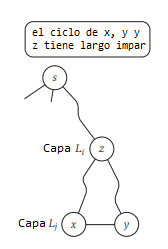
\includegraphics[scale=1]{Imagenes-Seccion3/3dot6.png}
\caption{Si dos nodos x e y en la misma capa están unidos por una arista, entonces el ciclo a través de x, y, y su ancestro común más bajo z tiene una longitud impar, lo que demuestra que el grafo no puede ser bipartito.}
\label{Fig36}
\end{figure}




\subsection{Conexión en grafos dirigidos}

Hasta ahora, hemos estado viendo problemás en grafos no dirigidos; ahora consideramos hasta qué punto estas ideas se trasladan al caso de los grafos dirigidos.\\

Recuerde que en un grafo dirigido, la arista $(u, v)$ tiene una dirección: va de $u$ a $v$. De esta manera, la relación entre $u$ y $v$ es asimétrica, y esto tiene efectos cualitativos sobre la estructura del grafo resultante . En la Sección 3.1, por ejemplo, hablamos de la World Wide Web como una instancia de un grafo dirigido grande y complejo cuyos nodos son páginas y cuyos aristas son hipervínculos. El acto de explorar la Web se basa en seguir una secuencia de aristas en este grafo dirigido; y la direccionalidad es crucial, ya que generalmente no es posible navegar "hacia atrás" siguiendo los hipervínculos en la dirección inversa.\\

Al mismo tiempo, una serie de definiciones y algoritmos básicos tienen análogos naturales en el caso dirigido. Esto incluye la presentación de la lista de adyacencia y algoritmos de búsqueda de grafos como BFS y DFS. Ahora discutimos estos a su vez.\\

\subsubsection*{Representando Grafos Dirigidos}

Para representar un grafo dirigido a los fines del diseño de algoritmos, utilizamos una versión de la representación de la lista de adyacencia que empleamos para los grafos no dirigidos. Ahora, en lugar de que cada nodo tenga una sola lista de vecinos, cada nodo tiene dos listas asociadas: una lista consta de nodos a los que tiene aristas, y una segunda lista consta de nodos desde los que tiene aristas. Por lo tanto, un algoritmo que actualmente está mirando un nodo puede leer los nodos accesibles yendo un paso adelante en una arista dirigido, así como también los nodos a los que se puede acceder si uno da un paso en la dirección contraria en una arista desde usted.\\

\subsubsection*{Algoritmos de búsqueda de grafos}

BFS y DFS son casi los mismos algoritmos en los grafos dirigidos que en los grafos no dirigidos. Nos enfocaremos aquí en BFS. Comenzamos en un nodo s, definimos una primera capa de nodos que consiste en todos aquellos a los que s tiene una arista, definimos una segunda capa que consta de todos los nodos adicionales a los que estos nodos de la primera capa tienen una arista, y así sucesivamente. De esta forma, descubrimos los nodos capa por capa tal como se alcanzan en esta búsqueda hacia afuera desde s, y los nodos en la capa j son precisamente aquellos para los cuales la ruta más corta desde s tiene exactamente j aristas. Como en el caso no dirigido, este algoritmo realiza a lo sumo un trabajo constante para cada nodo y arista, lo que da como resultado un tiempo de ejecución de O (m + n).\\

Es importante entender qué está procesando esta versión dirigida de BFS. En los grafos dirigidos, es posible que un nodo tenga una ruta a un nodo t aunque t no tenga una ruta hacia s; y lo que hace BFS en los grafos dirigidos es calcular es el conjunto de todos los nodos t con la propiedad s que tiene una ruta hacia t. Dichos nodos pueden tener o no caminos hacia s.\\

También existe un análogo a DFS, que también se ejecuta en tiempo lineal y calcula el mismo conjunto de nodos. Es de nuevo un procedimiento recursivo que trata de explorar lo más profundo ("deep") 
posible, en este caso solo siguiendo las aristas de acuerdo con su dirección inherente. Por lo tanto, cuando DFS se encuentra en un nodo $u$, inicia de forma recursiva una búsqueda en profundidad, en orden, para cada nodo al que $u$ tiene una arista.\\

Supongamos que, para un nodo dado s, queríamos el conjunto de nodos que tienen un camino a s, en lugar del conjunto de nodos a los que s tiene un camino a ellos. Una manera fácil de hacerlo sería definir un nuevo grafo dirigido, $G^{rev}$, que obtenemos de G simplemente invirtiendo la dirección de cada arista. Entonces podríamos ejecutar BFS o DFS en $G^{rev}$; un nodo tiene un camino desde s en $G^{rev}$ si y solo si tiene un camino a s en G.\\

\subsubsection*{Fuertemente conexo}


Recuerde que un grafo dirigido es fuertemente conexo si, por cada dos nodos $u$ y $v$, hay un camino de $u$ a $v$ y un camino de $v$ a $u$. También vale la pena formular una terminología para la propiedad en el corazón de esta definición; digamos que dos nodos $u$ y $v$ en un grafo dirigido son mutuamente alcanzables si hay un camino de $u$ a $v$ y también un camino de $v$ a $u$. (Entonces, un grafo es fuertemente conexo si cada par de nodos es mutuamente alcanzable).\\

 El alcance mutuo tiene una serie de buenas propiedades, muchas de ellas derivadas del siguiente enunciado.\\

\textbf{(3.16)} Si $u$ y $v$ son mutuamente alcanzables, y $v$ y $w$ son mutuamente alcanzables, entonces $u$ y $w$ son mutuamente alcanzables.\\

\textbf{Demostración}. Para construir un camino desde $u$ hasta $w$, primero pasamos de $u$ a $v$ (a lo largo del camino garantizado por el alcance mutuo de $u$ y $v$), y luego de $v$ a $w$ (a lo largo del camino garantizado por el alcance mutuo de $v$ y $w$). Para construir un camino de $w$ a $u$, simplemente invertimos este razonamiento: primero vamos de $w$ a $v$ (a lo largo del camino garantizado por el alcance mutuo de $v$ y $w$), y luego de $v$ a $u$ (a lo largo del camino garantizado por el alcance mutuo de $u$ y $v$). $\blacksquare$ \\

Hay un algoritmo simple de tiempo lineal para probar si un grafo dirigido es fuertemente conexo, implícitamente basado en $(3.16)$. Seleccionamos cualquier nodo y ejecutamos BFS en $G$ comenzando desde $s$. Luego también ejecutamos BFS comenzando desde $s$ en $G^{rev}$. Ahora, si una de estas dos búsquedas no llega a cada nodo, entonces claramente $G$ no es fuertemente conexo. Pero supongamos que encontramos que $s$ tiene un camino a cada nodo, y que cada nodo tiene un camino a $s$. Entonces $s$ y $v$ son mutuamente alcanzables para cada $v$, y por lo tanto se deduce que cada dos nodos $u$ y $v$ son mutuamente alcanzables: $s$ y $u$ son mutuamente alcanzables, y $s$ y $v$ son mutuamente alcanzables, entonces por (3.16) también tenemos eso $u$ y $v$ son mutuamente alcanzables.\\

Por analogía con las componentes conexas en un grafo no dirigido, podemos definir la componente fuertemente conexa que contiene un nodo $s$ en un grafo dirigido para que sea el conjunto de todos los $v$, de modo que $s$ y $v$ sean mutuamente alcanzables. Si uno lo piensa, el algoritmo en el párrafo anterior realmente está computando la componente fuertemente conexa que contiene $s$: ejecutamos BFS empezando por $s$ en $G$ y en $G^{rev}$; el conjunto de nodos al que alcanzan ambas búsquedas es el conjunto de nodos con caminos hacia y desde $s$, y por lo tanto este conjunto es la componente fuertemente conexa que contiene $s$.\\

Existen otras similitudes entre la noción de componentes conexas en grafos no dirigidos y componentes fuertemente conexas en grafos dirigidos. Recuerde que las componentes conexas dividen naturalmente el grafo, ya que dos componentes conexas eran idénticas o disjuntas. Las componentes fuertemente conexas también tienen esta propiedad, y por esencialmente la misma razón, basados en $(3.16)$.\\


 \colorbox{mygray}{\parbox{15cm}{
	\textbf{(3.17):}  Para dos nodos $s$ y $t$ en un grafo dirigido, sus componentes fuertemente conexas son idénticas o disjuntas.}}\\\\
    
\textbf{Prueba}. Considere dos nodos $s$ y $t$ que sean mutuamente alcanzables; afirmamos que las componentes fuertemete conexas que contienen $s$ y $t$ son idénticas. De hecho, para cualquier nodo $v$, si $s$ y $v$ son mutuamente alcanzables, entonces por $(3.16)$, $t$ y $v$ son mutuamente alcanzables también. De manera similar, si $t$ y $v$ son mutuamente alcanzables, entonces nuevamente por $(3.16)$, $s$ y $v$ son mutuamente alcanzables.\\

Por otro lado, si $s$ y $t$ no son mutuamente alcanzables, entonces no puede haber un nodo $v$ que esté en la componente fuertemente conexa de cada uno. Porque si hubiera tal nodo $v$, entonces $s$ y $v$ serían mutuamente alcanzables, y $v$ y $t$ serían mutuamente alcanzables, entonces desde $(3.16)$ se seguiría que $s$ y $t$ eran mutuamente alcanzables. $\blacksquare$\\

De hecho, aunque no vamos a discutir los detalles de esto aquí, con más trabajo es posible calcular las componentes fuertemente conexas para todos los nodos en un tiempo total de $O(m+n)$.\\


\subsection{Grafos acíclicos dirigidos y orden topológico}

Si un grafo no dirigido no tiene ciclos, entonces tiene una estructura extremadamente simple: cada uno de sus componentes conexas es un árbol. Pero es posible que un grafo dirigido no tenga ciclos (dirigidos) y aún tenga una estructura muy rica. Por ejemplo, tales grafos pueden tener una gran cantidad de aristas:\\

\begin{figure}[h]
\centering
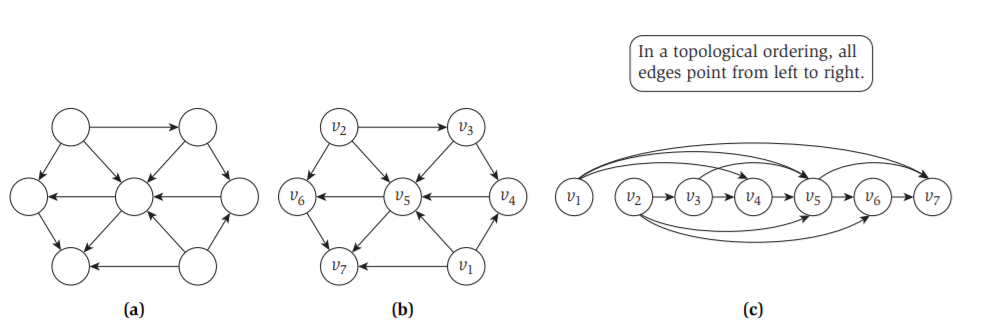
\includegraphics[scale=0.7]{Imagenes-Seccion3/fig3_4.PNG}
\caption{Figura 3.7 $(a)$ Un grafo acíclico dirigido. $(b)$ El mismo DAG con un orden topológico, especificado por las etiquetas en cada nodo. $(c)$ Un dibujo diferente del mismo DAG, dispuesto para enfatizar el orden topológico}
\end{figure}


Si establecemos el conjunto de nodos $\{1, 2,. . . , n\}$ e incluimos una arista $(i, j)$ siempre que $i <j$, entonces el grafo dirigido resultante tiene  \(\binom{n}{2}\) aristas pero no ciclos.\\

Si un grafo dirigido no tiene ciclos, lo llamamos, naturalmente, un grafo acíclico dirigido, o un DAG para abreviar. (El término DAG se pronuncia típicamente como una palabra, no se explica como un acrónimo.) En la figura 3.7 (a) vemos un ejemplo de un DAG, aunque puede requerir cierta comprobación para convencerse de que realmente no tiene ciclos dirigidos.\\


\subsubsection*{El Problema}

Los DAG son una estructura muy común en informática, porque muchos tipos de redes de dependencia del tipo que discutimos en la Sección 3.1 son acíclicos. Por lo tanto, los DAG se pueden usar para codificar relaciones o dependencias de precedencia de forma natural. Supongamos que tenemos un conjunto de tareas etiquetadas $\{1, 2,. . . , n\}$ que deben realizarse, y existen dependencias entre ellos que estipulan, para ciertos pares $i$ y $j$, que debo realizarme antes de $j$. Por ejemplo, las tareas pueden ser cursos, con requisitos previos que establecen que ciertos cursos deben tomarse antes que otros. O las tareas pueden corresponder a una cartera de trabajos informáticos, con afirmaciones de que la salida del trabajo $i$ se usa para determinar la entrada al trabajo $j$, y por lo tanto el trabajo debe realizarse antes del trabajo $j$.\\

Podemos representar un conjunto de tareas interdependientes introduciendo un nodo para cada tarea, y una arista dirigida $(i, j)$ siempre que deba hacerse antes de $j$. Si la relación de precedencia tiene que ser significativa, el grafo resultante $G$ debe ser un DAG. De hecho, si contuviera un ciclo $C$, no habría forma de realizar ninguna de las tareas en $C$: dado que cada tarea en $C$ no puede comenzar hasta que otra complete, ninguna tarea en $C$ podría realizarse, ya que no se podría hacer ninguna primero.\\

Continuemos un poco más con esta imagen de DAG como relaciones de precedencia. Dado un conjunto de tareas con dependencias, sería natural buscar un orden válido en el que se puedan realizar las tareas, para que se respeten todas las dependencias. Específicamente, para un grafo dirigido $G$, decimos que un ordenamiento topológico de G es un ordenamiento de sus nodos como $v_1, v_2, ..., v_n$ de modo que para cada arista $(v_i, v_j)$, tenemos $i <j$. En otras palabras, todas las aristas apuntan hacia adelante en el orden. Un orden topológico en las tareas proporciona un orden en el que se pueden realizar de forma segura; cuando llegamos a la tarea $v_j$, ya se han hecho todas las tareas que se requieren para precederla. En la figura 3.7 (b) hemos etiquetado los nodos del DAG de la parte (a) con un orden topológico; tenga en cuenta que cada arista realmente pasa de un nodo indexado más bajo a un nodo indexado más alto.\\

De hecho, podemos ver un ordenamiento topológico de $G$ como una "prueba" inmediata de que $G$ no tiene ciclos, a través de lo siguiente.\\

 \colorbox{mygray}{\parbox{15cm}{
	\textbf{(3.18):} Si $G$ tiene un orden topológico, entonces $G$ es un DAG}}\\\\

\textbf{Demostración:} Supongamos, por absurdo, que $G$ tiene un ordenamiento topológico $v_1, v_2, ..., v_n$, y también tiene un ciclo $C$. Sea$v_i$ el nodo indexado más bajo en $C$ y $v_j$ el nodo en $C$ justo antes de $v_i$ -así $(v_j, v_i)$ es una arista. Pero por nuestra elección de $i$, tenemos $j> i$, lo que contradice la suposición de que $v_1, v_2, ..., v_n$ era un ordenamiento topológico. $\blacksquare$\\

La prueba de aciclicidad que proporciona un ordenamiento topológico puede ser muy útil, incluso visualmente. En la Figura 3.7 (c), hemos dibujado el mismo grafo que en (a) y (b), pero con los nodos establecidos en el orden topológico. Está inmediatamente claro que el grafo en (c) es un DAG ya que cada arista va de izquierda a derecha\\

\textbf{Calcular un orden topológico} La pregunta principal que consideramos aquí es la inversa de $(3.18)$: ¿Todos los DAG tienen un orden topológico y, de ser así, cómo lo encontramos de manera eficiente? Un método para hacer esto para cada DAG sería muy útil: mostraría que para cualquier relación de precedencia en un conjunto de tareas sin ciclos, hay un orden eficientemente computable para realizar las tareas.\\

\subsubsection*{Diseñando y Analizando el Algoritmo}

De hecho, el inverso de (3.18) se mantiene, y lo establecemos a través de un algoritmo eficiente para calcular un ordenamiento topológico. La clave de esto radica en encontrar una manera de comenzar: ¿qué nodo ponemos al comienzo del ordenamiento topológico? Tal nodo $v_1$ no necesitaría aristas entrantes, ya que cualquier arista entrante violaría la propiedad de definición del ordenamiento topológico, que todas las aristas apuntan hacia adelante. Por lo tanto, tenemos que probar el siguiente hecho:\\

\paragraph{}
\colorbox{mygray}{\parbox{15cm}{
	\textbf{(3.19):} En cada DAG $G$, hay un nodo $v$ sin aristas entrantes.}}\\\\

  \textbf{Demostración:}. Sea $G$ un grafo dirigido en el que cada nodo tiene al menos una arista entrante. Mostraremos cómo encontrar un ciclo en $G$; esto probará lo que se quiere. Seleccionamos cualquier nodo $v$, y comenzamos a seguir las aristas hacia atrás desde $v$: ya que $v$ tiene al menos un arista entrante $(u, v)$, podemos caminar hacia atrás hasta $u$; entonces, dado que $u$ tiene al menos una arista entrante $(x, u)$, podemos retroceder hacia $x$; y así. Podemos continuar este proceso indefinidamente, ya que cada nodo que encontramos tiene una arista entrante. Pero después de $n+1$ pasos, habremos visitado algún nodo $w$ dos veces. Sea $C$ la secuencia de nodos encontrados entre las visitas sucesivas a $w$, entonces claramente $C$ forma un ciclo. $\blacksquare$\\

De hecho, la existencia de tal nodo $v$ es todo lo que necesitamos para producir un ordenamiento topológico de $G$ por inducción. Específicamente, aleguemos por inducción que cada DAG tiene un orden topológico. Esto es claramente cierto para los DAG en uno o dos nodos. Ahora supongamos que es cierto para DAG con hasta cierto número de nodos $n$. Luego, dado un DAG $G$ con $n + 1$ nodos, encontramos un nodo $v$ sin aristas entrantes, como lo garantiza $(3.19)$. Colocamos $v$ primero en el orden topológico; esto es seguro, ya que todos las aristas fuera de $v$ apuntarán hacia adelante. Ahora $G- \{v\}$ es un DAG, ya que al eliminar $v$ no se pueden crear ciclos que no estaban allí previamente. Además, $G- \{v\}$ tiene $n$ nodos, por lo que podemos aplicar la hipótesis de inducción para obtener un ordenamiento topológico de $G- \{v\}$ . Agregamos los nodos de $G- \{v\}$  en este orden después de $v$; este es un ordenamiento de $G$ en el que todos las aristas apuntan hacia adelante, y por lo tanto es un ordenamiento topológico.\\

Por lo tanto, hemos demostrado la afirmación deseada de $(3.18)$.\\


 \colorbox{mygray}{\parbox{15cm}{
	\textbf{(3.20):}  Si $G$ es un DAG, entonces $G$ tiene un orden topológico.}}\\\\

La prueba inductiva contiene el siguiente algoritmo para calcular un orden topológico de $G$.\\



\begin{lstlisting}
Para calcular un orden topologico de G:
Encuentre un nodo v sin aristas entrantes y ponga a v en el primer lugar
Eliminar v de G
Calcular recursivamente un ordenamiento topologico de G- {v} y agregue este orden despues de v
\end{lstlisting}

\begin{figure}[h]
\centering
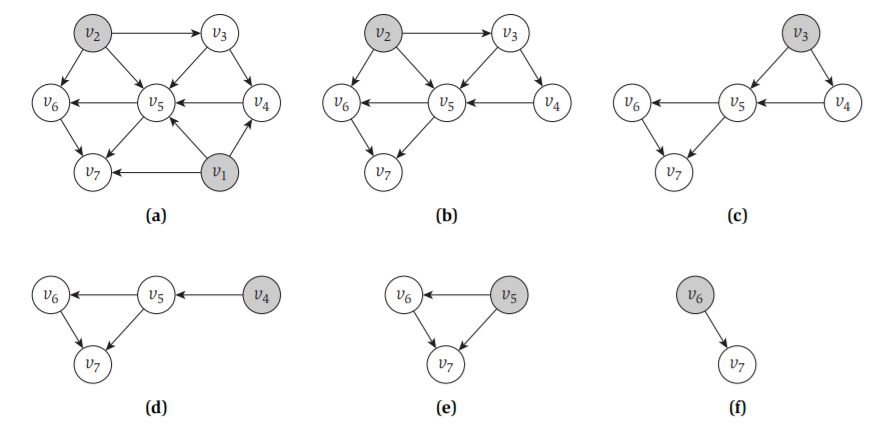
\includegraphics[scale=0.7]{Imagenes-Seccion3/fig3_8.PNG}
\caption{Figura 3.8: A partir del grafo de la Figura 3.7, los nodos se eliminan uno por uno para agregarse a un orden topológico. Los nodos sombreados son aquellos sin aristas entrantes; tenga en cuenta que siempre hay al menos uno de esos aristas en cada etapa de la ejecución del algoritmo}
\end{figure}


En la Figura 3.8 mostramos la secuencia de eliminaciones de nodo que ocurre cuando este algoritmo se aplica al grafo en la Figura 3.7. Los nodos sombreados en cada iteración son aquellos sin aristas entrantes; el punto crucial, que es lo que (3.19) garantiza, es que cuando aplicamos este algoritmo a un DAG, siempre habrá al menos un nodo disponible para eliminar.\\

Para vincular el tiempo de ejecución de este algoritmo, observamos que la identificación de un nodo $v$ sin aristas entrantes, y eliminarlo de $G$, se puede hacer en el tiempo $O(n)$. Como el algoritmo se ejecuta para $n$ iteraciones, el tiempo total de ejecución es $O(n^2)$.\\

Este no es un mal tiempo de ejecución; y si $G$ es muy denso, contiene $n^2$ aristas, entonces es lineal en el tamaño de la entrada. Pero es posible que deseemos algo mejor cuando la cantidad de aristas $m$ es mucho menor que $n^2$. En tal caso, un tiempo de ejecución de $O(m + n)$ podría ser una mejora significativa sobre $n^2$.\\

De hecho, podemos lograr un tiempo de ejecución de $O(m+n)$ usando el mismo algoritmo de alto nivel eliminando iterativamente nodos sin aristas entrantes. Simplemente tenemos que ser más eficientes para encontrar estos nodos, y lo hacemos de la siguiente manera\\

Declaramos que un nodo está "activo" si el algoritmo aún no lo ha eliminado, y explícitamente mantenemos dos cosas:\\

   \begin{enumerate}
   		\item para cada nodo $w$, la cantidad de aristas entrantes que $w$ tiene de los nodos activos; 
        \item y el conjunto $S$ de todos los nodos activos en $G$ que no tienen aristas entrantes de otros nodos activos.
   \end{enumerate}
    
Al principio, todos los nodos están activos, por lo que podemos inicializar (a) y (b) con una sola pasada a través de los nodos y las aristas. Luego, cada iteración consiste en seleccionar un nodo $v$ del conjunto $S$ y eliminarlo. Después de eliminar $v$, pasamos por todos los nodos $w$ a los que $v$ tiene una ventaja, y restamos uno del número de aristas entrantes activos que estamos manteniendo para $w$. Si esto hace que el número de aristas entrantes activos baje a cero, entonces agregamos $w$ al conjunto $S$. Procediendo de esta manera, hacemos un seguimiento de los nodos que son elegibles para borrado en todo momento, mientras gastamos trabajo constante por arista en el transcurso de todo el algoritmo.\\

\subsection{Ejercicios Resueltos}

\subsubsection*{Ejercicio 1}

Considere el grafo acíclico dirigido $G$ en la Figura 3.9. ¿Cuántas ordenaciones topológicas tiene?\\

\begin{figure}[h]
\centering
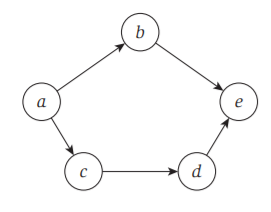
\includegraphics[scale=1.1]{Imagenes-Seccion3/fig3_9.PNG}
\caption{Figura 3.9 ¿Cuántas ordenaciones topológicas tiene este grafo?}
\end{figure}

\textbf{Solución:} Recuerde que un ordenamiento topológico de $G$ es un ordenamiento de los nodos como $v_1, v_2, ..., v_n$ de modo que todas las aristas apuntan hacia adelante: para cada arista $(v_i, v_j)$, tenemos $i <j$\\

Entonces, una forma de responder esta pregunta sería anotar todos los $5$x$4$x$3$x$2$x$1=120$ posibles ordenes y verificar si cada uno es un orden topológico. Pero esto tomaría un tiempo.\\

En cambio, pensamos en esto de la siguiente manera. Como vimos en el texto (o razonando directamente a partir de la definición), el primer nodo en un ordenamiento topológico debe ser uno que no tenga arista hacia él. Análogamente, el último nodo debe ser uno que no tenga arista que lo abandone. Por lo tanto, en cada orden topológico de $G$, el nodo $a$ debe ser el primero y el nodo $e$ debe ser el último.\\

Ahora tenemos que calcular cómo se pueden organizar los nodos $b$, $c$ y $d$ en el medio del pedido. La arista $(c, d)$ impone el requisito de que $c$ debe venir antes de $d$; pero $b$ puede colocarse en cualquier lugar en relación con estos dos: antes de ambos, entre $c$ y $d$, o después de ambos. Esto agota todas las posibilidades, por lo que concluimos que hay tres posibles ordenamientos topológicos: $\{a,b,c,d,e\}$, $\{a, c, b, d, e\}$ $\{a, c, d, b, e\}$\\

\subsubsection*{Ejercicio 2}

Algunos amigos tuyos están trabajando en técnicas para coordinar grupos de robots móviles. Cada robot tiene un transmisor de radio que utiliza para comunicarse con una estación base, y tus amigos encuentran que si los robots se acercan demásiado el uno al otro, entonces hay problemás con la interferencia entre los transmisores. De modo que surge un problema natural: cómo planificar el movimiento de los robots de modo que cada robot llegue a su destino previsto, pero en el proceso los robots no se acercan lo suficiente como para causar problemás de interferencia.\\

Podemos modelar este problema de forma abstracta de la siguiente manera. Supongamos que tenemos un grafo no dirigido $G =(V, E)$, que representa el plano de un edificio, y hay dos robots ubicados inicialmente en los nodos $a$ y $b$ en el grafo. El robot en el nodo $a$ quiere viajar al nodo $c$ a lo largo de un camino en $G$, y el robot en el nodo $b$ quiere viajar al nodo $d$. Esto se logra por medio de un cronograma: en cada paso de tiempo, el cronograma especifica que uno de los robots se mueve a través de una única arista, de un nodo $a$ un nodo vecino; al final del programa, el robot del nodo $a$ debe estar sentado en $c$, y el robot de $b$ debe estar sentado en $d$.\\

Un programa es libre de interferencias si no hay ningún punto en el que los dos robots ocupen nodos que están a una distancia $≤ r$ uno del otro en el grafo, para un parámetro dado $r$. Supondremos que los dos nodos iniciales $a$ y $b$ están a una distancia mayor que $r$, y también lo son los dos nodos finales $c$ y $d$.\\

Proporcione un algoritmo de tiempo polinomial que decida si existe un cronograma sin interferencias mediante el cual cada robot pueda llegar a su destino\\

\textbf{Solución:} Este es un problema del siguiente sabor general. Tenemos un conjunto de configuraciones posibles para los robots, donde definimos una configuración para que sea una elección de ubicación para cada uno. Estamos tratando de llegar desde una configuración inicial dada $(a,b)$ a una configuración final dada $(c,d)$, sujeta a restricciones sobre cómo podemos movernos entre configuraciones (solo podemos cambiar la ubicación de un robot a un nodo vecino), y también sujeto a restricciones sobre qué configuraciones son "legales".\\

Este problema puede ser difícil de considerar si vemos las cosas en el nivel del grafo subyacente $G$: para una configuración dada de los robots, es decir, la ubicación actual de cada uno, no está claro qué regla deberíamos usar para decidir cómo mover uno de los robots a continuación. Entonces, en su lugar, aplicamos una idea que puede ser muy útil para las situaciones en las que intentamos realizar este tipo de búsqueda. Observamos que nuestro problema se parece mucho a un problema de búsqueda de camino, no en el grafo original $G$ sino en el espacio de todas las configuraciones posibles.\\

Definamos el siguiente grafo (más grande) $H$. El conjunto de nodos de $H$ es el conjunto de todas las configuraciones posibles de los robots; es decir, $H$ consta de todos los pares posibles de nodos en $G$. Unimos dos nodos de $H$ por una arista si representan configuraciones que podrían ser consecutivas en un cronograma; es decir, $(u,v)$ y $(u',v')$ se unirán por una arista en $H$ si uno de los pares $u$, $u'$ o $v$, $v'$ son iguales, y el otro par corresponde a una arista en $G$.\\

Ya podemos observar que las trayectorias en $H$ de $(a,b)$ a $(c,d)$ corresponden a las programaciones de los robots: un camino así consiste precisamente en una secuencia de configuraciones en la que, en cada paso, un robot cruza una sola arista en $G$. Sin embargo, todavía no hemos codificado la noción de que el cronograma debe estar libre de interferencias.\\

Para hacer esto, simplemente eliminamos de $H$ todos los nodos que corresponden a las configuraciones en las que habría interferencia. Por lo tanto, definimos $H'$ como el grafo obtenido de $H$ al eliminar todos los nodos $(u,v)$ para los cuales la distancia entre $u$ y $v$ en $G$ es como máximo $r$\\

El algoritmo completo es el siguiente. Construimos el grafo $H'$, y luego ejecutamos el algoritmo de conexidad que vimos antes para determinar si hay un camino desde $(a,b)$ a $(c,d)$. La corrección del algoritmo se deriva del hecho de que las trayectorias en $H'$ corresponden a las programaciones, y los nodos en $H'$ corresponden precisamente a las configuraciones en las que no hay interferencia.\\

Finalmente, debemos considerar el tiempo de ejecución. Denotemos a $n$ como el número de nodos en $G$, y $m$ el número de aristas en $G$. Analizaremos el tiempo de ejecución haciendo tres cosas: (1) acotando el tamaño de $H'$ (que en general será mayor que $G$), (2) acotando el tiempo que lleva construir $H'$, y (3) acotando el tiempo que lleva buscar un camino de $(a,b)$ a $(c,d)$ en $H$.\\

   \begin{enumerate}
   		\item Primero, entonces, consideremos el tamaño de $H'$. $H'$ tiene como máximo $n^2$ nodos, ya que sus nodos corresponden a pares de nodos en $G$. Ahora, ¿cuántas aristas tiene $H'$? Un nodo $(u,v)$ tendrá aristas a $(u',v)$ para cada vecino $u'$ de $u$ en $G$, y a $(u, v')$ para cada vecino $v'$ de $v$ en $G$. Una cota superior simple dice que puede haber a lo sumo $n$ opciones para $(u',v)$, y como mucho $n$ opciones para $(u,v')$, por lo que hay como máximo $2n$ aristas incidentes para cada nodo de $H'$. Sumando sobre los (como máximo) $n^2$ nodos de $H'$, tiene $O(n^3)$ aristas.\\
        
(En realidad podemos dar un mejor límite de $O(mn)$ en el número de aristas en $H'$, usando el límite (3.9) que probamos en la Sección 3.3 sobre la suma de los grados en un grafo. Lo dejaremos como un ejercicio adicional.)\\        
        
        
        \item Ahora limitamos el tiempo necesario para construir $H'$. Primero construimos $H$ enumerando todos los pares de nodos en $G$ en el tiempo $O(n^2)$ y construyendo aristas usando la definición anterior en el tiempo $O(n)$ por nodo, para un total de $O(n^3)$. Ahora necesitamos averiguar qué nodos eliminar de $H$ para producir $H'$. Podemos hacer esto de la siguiente manera. Para cada nodo $u$ en $G$, ejecutamos BFS($u$) e identificamos todos los nodos $v$ dentro de la distancia $r$ de $u$. Enumeramos todos estos pares $(u,v)$ y los eliminamos de $H$. Cada BFS en $G$ toma tiempo $O(m+n)$, y estamos haciendo uno desde cada nodo, por lo que el tiempo total para esta parte es $O(mn+n^2)$.
        \item Ahora tenemos $H'$, por lo que solo tenemos que decidir si hay un camino desde $(a,b)$ hasta $(c,d)$. Esto se puede hacer utilizando el algoritmo de conexidad del texto en el tiempo que es lineal en el número de nodos y aristas de $H'$. Como $H'$ tiene $O(n^2)$ nodos y $O(n^3)$ aristas, este paso final también toma tiempo polinómico.
\end{enumerate}


\begin{figure}[h]
\centering
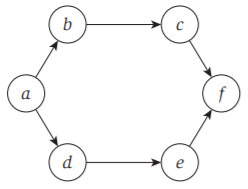
\includegraphics[scale=1.1]{Imagenes-Seccion3/fig3_10.PNG}
\caption{Figura 3.10 ¿Cuántas ordenaciones topológicas tiene este grafo?}
\end{figure}

\newpage

\section{Algoritmo voraz}


En Wall Street, esa icónica película de la década de 1980, Michael Douglas se incorpora
frente a una habitación llena de accionistas y proclama: " Codicia. . . es buena. La codicia
está bien. La codicia funciona". En este capítulo, tomaremos un enfoque mucho más discreto y perspectiva a medida que investigamos los pros y los contras de la codicia a corta alcance en el diseño de algoritmos. De hecho, nuestro objetivo es acercarnos a una serie de diferentes problemás computacionales con un conjunto de preguntas recurrentes: ¿es buena la codicia? ¿funciona?\\

Es difícil, si no imposible, definir con precisión lo que significa un algoritmo ávido. Un algoritmo es ávido si construye una solución en pequeños pasos, eligiendo una decisión en cada paso de corto alcance para optimizar algunos criterios subyacentes . A menudo se pueden diseñar muchos algoritmos ávidos diferentes para el mismo problema, cada uno localmente, optimizando incrementalmente en alguna medida diferente, mientras se llega a una solución.\\

Cuando un algoritmo ávido logra resolver un problema no trivial de manera óptima, típicamente implica algo interesante y útil sobre la estructura del problema en sí mismo; hay una regla de decisión local que uno puede usar para construir soluciones óptimás. Y como veremos más adelante, en el Capítulo 11, en ciertos problemás en los que un algoritmo ávido puede producir una solución que está garantizada que va a estar cerca de lo óptimo, incluso si no alcanza el óptimo preciso. Estos son los tipos de problemás que trataremos en este capítulo. Es fácil de inventar algoritmos ávido para casi cualquier problema y encontrar casos en los que funcionan bien, probar que funcionan bien, es el desafío interesante.\\

Las dos primeras secciones de este capítulo desarrollarán dos métodos básicos para demostrar que un algoritmo ávido produce una solución óptima a un problema. Uno puede ver el primer enfoque como establecer que el algoritmo ávido se mantiene adelante. Con esto queremos decir que si uno mide el progreso del algoritmo ávido paso a paso, uno ve que lo hace mejor que cualquier otro algoritmo en cada paso; luego se deduce que produce una solución óptima. El segundo enfoque se conoce como un argumento de intercambio, y es más general: uno considera cualquier posible solución al problema y lo transforma gradualmente en la solución encontrada por el algoritmo ávido sin dañar su calidad. De nuevo, se deduce que el algoritmo ávido debe haber encontrado una solución que es al menos tan bueno como cualquier otra solución.\\

Luego de nuestra introducción de estos dos estilos de análisis, nos enfocaremos en varias de las aplicaciones más conocidas de algoritmos ávidos: $shortest$ $paths$ $in$ $a$ $graph$ (el camino más corto en grafos), $the$ $Minimum$ $Spanning$ $Tree$ $Problem$ (el problema del árbol recubridor mínimo), y la construccion de $Huffman$ $codes$ para realizar la compresión de datos. Cada uno proporciona buenos ejemplos de nuestras técnicas de análisis. También exploraremos una relación interesante entre los árboles de recubrimiento mínimo y el muy estudiado problema de agrupamiento. Finalmente, consideraremos una aplicación más compleja, $Minimum-$ $Cost$ $Arborescence$ $Problem$ (problema de arborescencia de costo mínimo), que amplía aún más nuestra noción de lo ávido que el algoritmo es.\\


\subsection{Planificacion de intervalos: el algoritmo ávido se mantiene adelante} Recordemos el problema de planificacion de intervalos, que fue el primero de los cinco problemás representativos que consideramos en el Capítulo 1. Tenemos un conjunto de solicitudes ${1, 2,. . . , n}$; la $i- esima$ solicitud corresponde a un intervalo de tiempo que comienza en $s(i)$ y terminando en $f (i)$. (Tenga en cuenta que estamos cambiando ligeramente la notación de Sección 1.2, donde usamos $s_i$ en lugar de $s(i)$ y $f_i$ en lugar de $f(i)$. Este cambio de notación hará que las cosas sean más fáciles de hablar en las pruebas). Diremos que un subconjunto de las solicitudes es $compatible$ si no se superponen dos de ellas en un mismo tiempo, y nuestro objetivo es aceptar un subconjunto compatible tan grande como sea posible. Los conjuntos compatibles de tamaño máximo se denominarán \textit{óptimos}.\\

\subsubsection*{Diseñando un Algoritmo Ávido}

Usando el problema de planificacion de intervalos, podemos hacer nuestra discusión sobre algoritmos ávidos mucho más concreta. La idea básica en un algoritmo ávido para la planificación por intervalos es usar una regla simple para seleccionar una primera solicitud $i_1$. Una vez se acepta una solicitud $i_1$, rechazamos todas las solicitudes que no son compatibles con $i_1$. Luego seleccionamos la siguiente solicitud $i_2$ para ser aceptada, y rechazamos nuevamente todas las solicitudes que no son compatibles con $i_2$. Continuamos de esta manera hasta que acabemos con las solicitudes. El desafío al diseñar un buen algoritmo ávido es decidir qué regla simple usar para la selección, y hay muchas reglas naturales para este problema que no dan buenas soluciones.\\

Tratemos de pensar en algunas de las reglas más naturales y ver cómo funcionan.\\

\begin{itemize}
\item 	La regla más obvia puede ser seleccionar siempre la primer solicitud disponible, es decir el que tiene un tiempo mínimo de inicio $s(i)$. De esta forma nuestro recurso comienza a ser utilizado lo más rápido posible.\\
\end{itemize}

Este método no produce una solución óptima. Si la primera solicitud $i$ es por un intervalo muy largo, luego al aceptar la solicitud, podemos tener que rechazar una gran cantidad de solicitudes de intervalos de tiempo más cortos. Dado que nuestro objetivo es satisfacer tantas solicitudes como sea posible, terminaremos con una solución subóptima.\\

En un caso realmente malo, por ejemplo, cuando el tiempo de finalización $f(i)$ es el máximo entre todas las solicitudes: la solicitud aceptada mantendrá nuestro recurso ocupado por todo el tiempo En este caso, nuestro método ávido aceptaría solo una solicitud, mientras que la solución óptima podría aceptar muchas solicitudes. Tal situación está representado en la Figura 4.1 (a).
\begin{itemize}
\item	Esto podría sugerir que deberíamos comenzar aceptando la solicitud que requiere el menor intervalo de tiempo, es decir, la solicitud para la cual $f(i) - s(i)$ es lo más pequeña posible. Como resultado, esto es una regla mejor que la anterior, pero aún puede producir un horario subóptimo. Por ejemplo, en la Figura 4.1 (b), aceptando el intervalo corto en el medio nos impediría aceptar los otros dos, que forman una solución óptima.\\
\end{itemize}

\begin{figure}[h]
\centering
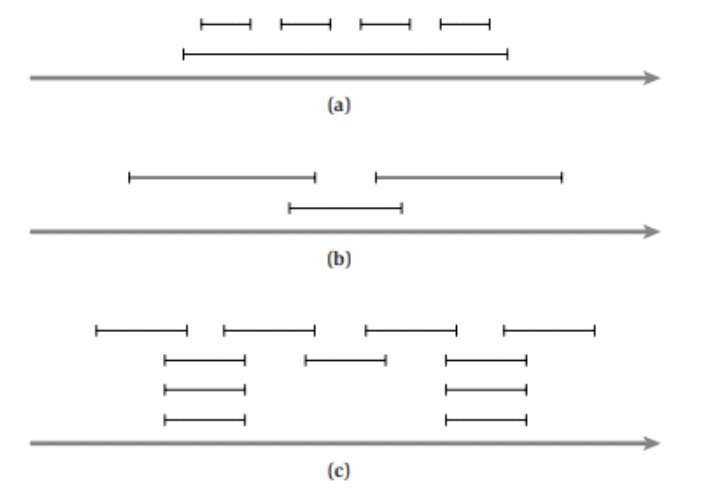
\includegraphics[scale=0.7]{Imagenes-Seccion4/fig4_1.PNG}
\caption{Figura 4.1 Algunas instancias del problema de planificación de intervalos en el que los algoritmos ávidos naturales no logran encontrar la solución óptima. En (a), no funciona seleccionar el intervalo que comienza más temprano; en (b), no funciona seleccionar el intervalo más corto; y en (c), no funciona seleccionar el intervalo con el menor número de conflictos.}
\end{figure}

\begin{itemize}
\item	 En la regla ávida anterior, nuestro problema era que la segunda solicitud compite con la primera y la tercera solicitud, es decir, aceptar esta solicitud nos hizo rechazar otras dos solicitudes. Podríamos diseñar un algoritmo ávido que se basa en esta idea: para cada solicitud, contamos el número de otras solicitudes que no son compatibles, y acepta la solicitud que tiene el menor número de solicitudes no compatibles. (En otras palabras, seleccionamos el intervalo con el menor número de " conflictos"). Esta regla ávida de elección conduciría a la solución óptima en el ejemplo anterior. De hecho, es un poco más difícil diseñar un mal ejemplo para esta regla; pero se puede hacer, y hemos dibujado un ejemplo en la Figura 4.1 (c). La solución óptima única en este ejemplo es aceptar las cuatro solicitudes en la fila superior. Los métodos ávidos sugeridos aquí aceptan la solicitud del medio en la segunda fila y por lo tanto, garantizan una solución de tamaño no superior a tres.\\

Una regla ávida que conduce a la solución óptima se basa en una cuarta idea: primero debemos aceptar la solicitud que termina primero, es decir, la solicitud $i$ para lo cual $f (i)$ es lo más pequeño posible. Esta es también una idea bastante natural: nos aseguramos que nuestro recurso se libera lo antes posible sin dejar de satisfacer una solicitud. De esta forma, podemos maximizar el tiempo restante para satisfacer otras solicitudes.\\

Vamos a establecer un algoritmo un poco más formal. Usaremos $R$ para denotar el conjunto de solicitudes que aún no hemos aceptado ni rechazado, y usamos $A$ para denotar el conjunto de solicitudes aceptadas. Para ver un ejemplo de cómo el algoritmo funciona, ver Figura 4.2.\\

\begin{lstlisting}
Sea R el conjunto de solicitudes y A un conjunto vacio
While R distinto de vacio
 Sea i en R / i tiene el tiempo de terminacion mas chico
 Agregar i a A
 Eliminamos de R las solicitudes incompatibles con i
EndWhile
return A como el conjunto de solicitudes aceptadas
\end{lstlisting}

\end{itemize}




\subsubsection*{Analizando el algoritmo}

Si bien este método ávido es bastante natural, ciertamente no es obvio que devuelve un conjunto óptimo de intervalos. De hecho, sería sensato reservar juicio sobre su optimalidad: las ideas que llevaron a la anterior versión no óptima del método ávido también parecían prometedoras al principio.\\

Para empezar, podemos declarar inmediatamente que los intervalos en el conjunto $A$ devueltos por el algoritmo son todos compatibles.\\

\textbf{(4.1)} A es un conjunto de solicitudes compatibles.\\


\begin{figure}[h]
\centering
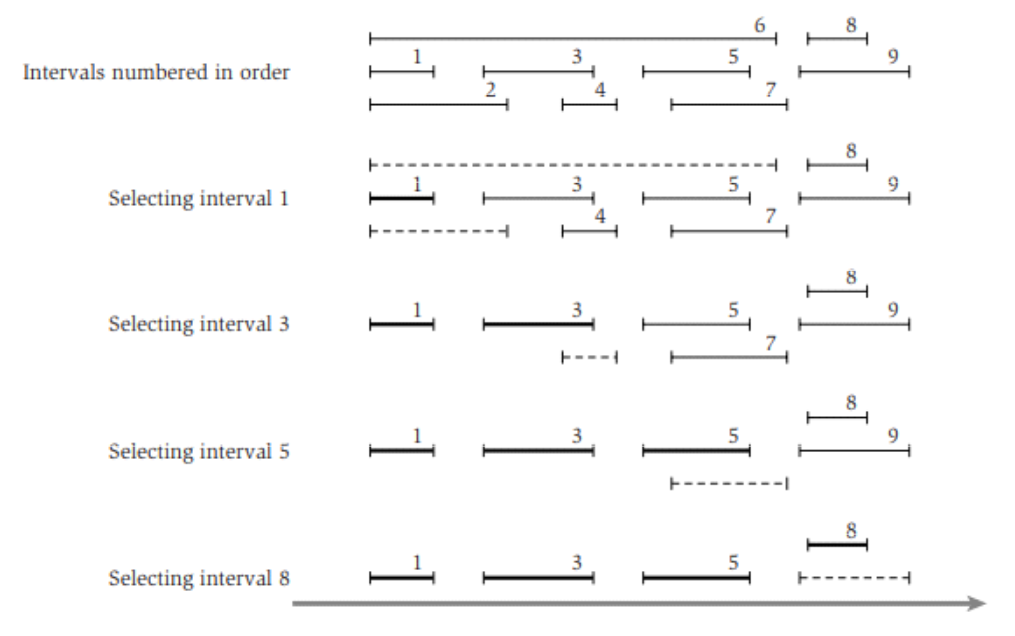
\includegraphics[scale=0.7]{Imagenes-Seccion4/fig4_2.PNG}
\caption{Figura 4.2 Ejecución de muestra del algoritmo de planificación de intervalos. En cada paso, el seleccionado de los intervalos son líneas más oscuras, y los intervalos eliminados en el paso correspondiente son indicado con líneas discontinuas.}
\end{figure}

Lo que necesitamos mostrar es que esta solución es óptima. Entonces, para propósitos de comparación, sea $O$ un conjunto óptimo de intervalos. Lo ideal es que uno quiera mostrar que $A = O$, pero esto es demásiado pedir: puede haber muchas soluciones óptimás, y en el mejor de los casos $A$ es igual a solo una de las soluciones. Entonces, en su lugar, implemente mostraremos que $|A| = |O|$, es decir, que $A$ contiene el mismo número de intervalos que $O$ y por lo tanto, también es una solución óptima.\\

La idea que subyace a la prueba, como sugerimos inicialmente, será encontrar un sentido en el que nuestro algoritmo ávido "se mantenga" por delante de esta solución $O$. Compararemos las soluciones parciales que el algoritmo ávido construye con los segmentos iniciales de la solución $O$, y demostrar que el algoritmo ávido está mejorando paso a paso.\\

Introducimos algunas notaciones para ayudar con esta prueba. Sea  $i_1, ...,i_k$ el conjunto de solicitudes en $A$ en el orden en que se agregaron a $A$. Tenga en cuenta que $|A| = k$. De manera similar, el conjunto de solicitudes en $O$ es denotado por $j_1, ...,j_m$. Nuestro objetivo es demostrar que $k = m$. Supongamos que las solicitudes de los intervalos correspondientes en $O$ también se ordenan en el orden natural de izquierda a derecha , es decir, en el orden de los puntos de inicio y fin. Tenga en cuenta que las solicitudes en $O$ son compatibles, lo que implica que los puntos de inicio tienen el mismo orden que los puntos finales.\\

\begin{figure}[h]
\centering
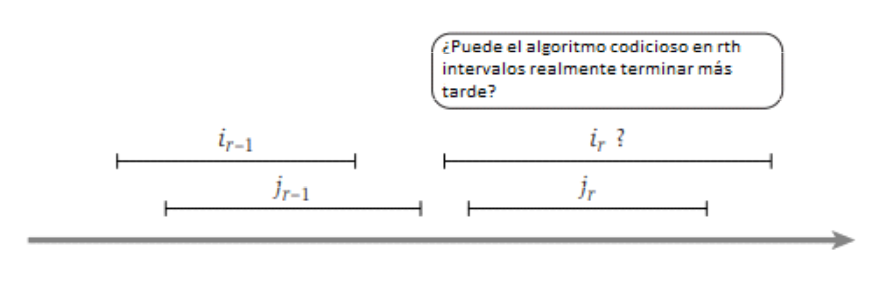
\includegraphics[scale=0.7]{Imagenes-Seccion4/fig4_3.PNG}
\caption{Figura 4.3 El paso inductivo en la prueba de que el algoritmo ávido se mantiene por delante.}
\end{figure}



Nuestra intuición para el método ávido vino de desear que nuestro recurso volviera a ser libre tan pronto como fuera posible después de satisfacer la primera solicitud. Y, de hecho, nuestra regla ávida garantiza que $f(i_1)≤ f(j_1)$. Este es el sentido en el cual queremos mostrar que nuestra regla ávida "se mantiene por delante", que cada uno de sus intervalos finaliza al menos tan pronto como el intervalo correspondiente en el conjunto $O$. Por lo tanto, ahora demostramos que para cada $r≥1$, la $r-esima$ solicitud aceptada en la planificación del algoritmo finaliza a más tardar igual tiempo que la solicitud $r-esima$ de la planificación óptima.\\

\textbf{(4.2)} Para todos los índices $r ≤ k$ tenemos que $f (i_r) ≤ f (j_r)$.\\


\textbf{Demostración}. Vamos a probar esta afirmación por inducción. Para $r=1$, la afirmación es claramente cierta: el algoritmo comienza seleccionando la solicitud $i_1$ con un tiempo mínimo de finalización.\\

Ahora, $r>1$. Asumiremos como nuestra hipótesis de inducción que la afirmación es verdadera para $r-1$, y trataremos de probarlo para $r$. Como se muestra en la Figura 4.3, la hipótesis de inducción nos permite suponer que $f(i_{r-1}) ≤ f(j_{r-1})$. Para que el intervalo $r-esimo$ del algoritmo no termine antes también, tendría que "quedarse atrás " como se muestra. Pero hay una razón simple por la que esto no podría suceder: en lugar de elegir un intervalo de finalización posterior, el algoritmo ávido siempre tiene la opción (en el peor caso) de elegir $j_r$ y así cumplir el paso de inducción.\\

Podemos hacer preciso este argumento de la siguiente manera. Sabemos (dado que $O$ consiste en intervalos compatibles) que $f(j_{r-1}) ≤ s(j_r)$. Combinando esto con la hipótesis de inducción $f(i_{r-1}) ≤ f(j_{r-1})$, obtenemos $f(i_{r-1}) ≤ s(j_r)$. Por lo tanto, el intervalo $j_r$ está en el conjunto $R$ de los intervalos disponibles en el momento en que el algoritmo ávido selecciona $i_r$. El algoritmo ávido selecciona el intervalo disponible con el menor tiempo de finalización; dado que el intervalo $j_r$ es uno de estos intervalos disponibles, tenemos $f(i_r) ≤ f(j_r)$. Con esto se completa el paso inductivo.  $\blacksquare$\\

Así, hemos formalizado el sentido en el que el algoritmo ávido permanece por delante de $O$: por cada $r$, el último intervalo que selecciona finaliza al menos tan pronto como el último intervalo en O. Ahora vemos por qué esto implica la optimalidad del algoritmo ávido que establece a $A$.\\

\colorbox{mygray}{\parbox{15cm}{
	\textbf{(4.3)}  El algoritmo ávido devuelve un conjunto óptimo $A$.}}\\\\


\textbf{Demostración}. Vamos a probar el enunciado por contradicción. Si $A$ no es óptimo, entonces un conjunto óptimo $O$ debe tener más solicitudes, es decir, debemos tener $m>k$. Aplicando (4.2) con $r = k$, obtenemos que $f(i_k) ≤ f(j_k)$. Como $m>k$, hay una solicitud $j_{k + 1}$ en $O$. Esta solicitud se inicia después de que la solicitud $j_k$ finaliza, y por lo tanto, después de que $i_k$ finaliza. Entonces, después de eliminar todas las solicitudes que no son compatibles con las solicitudes $i_1, ..., i_k$, el conjunto de posibles solicitudes $R$ todavía contiene $j_{k + 1}$. Pero el algoritmo ávido se detiene con la solicitud $i_k$, y solo se detiene cuando $R$ está vacío, una contradicción.  $\blacksquare$\\

\textbf{Implementación y tiempo de ejecución.} Podemos hacer que nuestro algoritmo se ejecute en el tiempo $O(nlogn)$ de la siguiente manera. Comenzamos ordenando las $n$ solicitudes en orden de tiempo de finalización y etiquetándolas en este orden; es decir, asumiremos que $f(i) ≤ f(j)$ cuando $i<j$. Esto lleva tiempo $O(nlogn)$. En un tiempo $O(n)$ adicional, construimos el array $S[1...n]$ con la propiedad de que $S[i]$ contiene el valor $s(i)$.\\

Ahora seleccionamos las solicitudes procesando los intervalos en orden de $f(i)$ creciente. Siempre seleccionamos el primer intervalo; luego iteramos a través de los intervalos en orden hasta alcanzar el primer intervalo $j$ para el cual $s(j) ≥ f(1)$; luego seleccionamos este también. De manera más general, si el intervalo más reciente que hemos seleccionado finaliza en el tiempo $f$, continuaremos iterando a través de intervalos posteriores hasta llegar a la primera $j$ para la cual $s(j) ≥ f$. De esta forma, implementamos el algoritmo ávido analizado anteriormente en una pasada a través de los intervalos, pasando un tiempo constante por intervalo. Por lo tanto, esta parte del algoritmo toma tiempo $O(n)$.\\

\subsubsection*{Extensiones}

El problema de planificación de intervalos que consideramos aquí es un problema de planificación bastante simple. Hay muchas otras complicaciones que podrían surgir en entornos prácticos. Los siguientes puntos señalan los problemás que veremos más adelante en el libro en varias formás.\\

    • Al definir el problema, supusimos que todas las solicitudes eran conocidas por el algoritmo de planificación cuando estaba eligiendo el subconjunto compatible. También sería natural, por supuesto, pensar en la versión del problema en la que el planificador necesita tomar decisiones sobre la aceptación o el rechazo de ciertas solicitudes antes de conocer el conjunto completo de solicitudes. Los clientes (solicitantes) pueden ser impacientes y pueden darse por vencidos y marcharse si el planificador espera demásiado tiempo para reunir información sobre todas las demás solicitadas. Un área activa de investigación se refiere a tales algoritmos en línea, que deben tomar decisiones a medida que transcurre el tiempo, sin conocimiento de la entrada futura.\\

    • Nuestro objetivo era maximizar el número de solicitudes satisfechas. Pero podríamos imaginar una situación en la que cada solicitud tiene un valor diferente para nosotros. Por ejemplo, cada solicitud también podría tener un valor $v_i$ (la cantidad obtenida al satisfacer la solicitud $i$), y el objetivo sería maximizar nuestros ingresos: la suma de los valores de todas las solicitudes satisfechas. Esto lleva al problema de planificación de intervalos ponderados, el segundo de los problemás representativos que describimos en el Capítulo 1.\\

Hay muchas otras variantes y combinaciones que pueden surgir. Ahora discutimos una de estas variantes adicionales con más detalle, ya que forma otro caso en el que un algoritmo ávido se puede utilizar para producir una solución óptima.\\

\subsection{Problema relacionado: planificar todos los intervalos}

\textbf{El problema} En el problema de planificación de intervalos, hay un único recurso y muchas solicitudes en forma de intervalos de tiempo, por lo que debemos elegir qué solicitudes aceptar y cuáles rechazar. Surge un problema relacionado si tenemos muchos recursos idénticos disponibles y deseamos planificar todas las solicitudes usando la menor cantidad de recursos posible. Debido a que el objetivo aquí es dividir todos los intervalos en múltiples recursos, nos referiremos a esto como el Problema de Partición de Intervalos.\\

El problema también se conoce como el problema de coloración por intervalos; la terminología surge de pensar que los diferentes recursos tienen distintos colores: a todos los intervalos asignados a un recurso particular se les da el color correspondiente.\\

Por ejemplo, suponga que cada solicitud corresponde a una conferencia que debe programarse en un aula durante un intervalo de tiempo determinado. Deseamos satisfacer todas estas solicitudes, utilizando el menor número de aulas posible. Las aulas a nuestra disposición son, por lo tanto, los recursos múltiples, y la restricción básica es que dos conferencias que se superponen en el tiempo deben programarse en diferentes aulas. De forma equivalente, las solicitudes de intervalo podrían ser trabajos que deben procesarse durante un período de tiempo específico, y los recursos son máquinas capaces de manejar estos trabajos. Mucho más adelante en el libro, en el Capítulo 10, veremos una aplicación diferente de este problema en la que los intervalos son solicitudes de enrutamiento a las que se debe asignar ancho de banda en un cable de fibra óptica. \\

Como ilustración del problema, considere la instancia de muestra en la Figura 4.4 (a). Las solicitudes en este ejemplo se pueden planificar utilizando tres recursos; esto se indica en la Figura 4.4 (b), donde las solicitudes se reorganizan en tres filas, cada una con un conjunto de intervalos no superpuestos. En general, se puede imaginar una solución que utiliza recursos $k$ como una reorganización de las solicitudes en $k$ filas de intervalos no superpuestos: la primera fila contiene todos los intervalos asignados al primer recurso, la segunda fila contiene todos los asignados al segundo recurso, y así sucesivamente.\\


\begin{figure}[h]
\centering
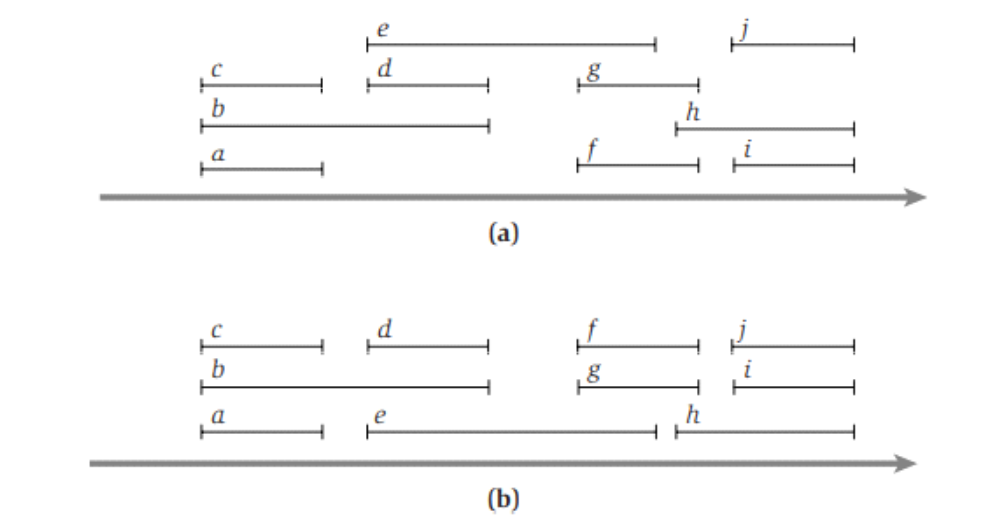
\includegraphics[scale=0.7]{Imagenes-Seccion4/fig4_4.PNG}
\caption{Figura 4.4 (a) Una instancia del problema de particiones por intervalos con diez intervalos (de la $a$ a la $j$). (b) Una solución en la que todos los intervalos se planifican utilizando tres recursos: cada fila representa un conjunto de intervalos que se pueden planificar en un solo recurso.}
\end{figure}

Ahora, ¿ hay alguna esperanza de usar solo dos recursos en esta instancia de muestra? Claramente la respuesta es no. Necesitamos al menos tres recursos, ya que, por ejemplo, los intervalos $a$, $b$ y $c$ pasan todos sobre un punto común en la línea de tiempo, y por lo tanto, todos deben programarse en recursos diferentes. De hecho, uno puede hacer este último argumento en general para cualquier instancia de Intervalo de Partición. Supongamos que definimos la profundidad de un conjunto de intervalos como el número máximo que pasa sobre un único punto en la línea de tiempo. Entonces decimos:\\

(4.4) En cualquier instancia de Intervalo de Partición, la cantidad de recursos necesarios es al menos la profundidad del conjunto de intervalos.\\

\textbf{Demostración}. Supongamos que un conjunto de intervalos tiene profundidad $d$, y que $I_1, ..., I_d$ pasan todos sobre un punto común en la línea de tiempo. Entonces cada uno de estos intervalos debe planificarse en un recurso diferente, por lo que toda la instancia juntas necesitan al menos $d$ recursos simultáneamente.  $\blacksquare$\\

Ahora consideramos dos preguntas, que están estrechamente relacionadas. En primer lugar, ¿ podemos diseñar un algoritmo eficiente que planifique todos los intervalos utilizando la mínima cantidad posible de recursos? En segundo lugar, ¿siempre hay un horario que utiliza una cantidad de recursos igual a la profundidad? En efecto, una respuesta positiva a esta segunda pregunta diría que los únicos obstáculos para los intervalos de partición son puramente locales: un conjunto de intervalos todos apilados sobre el mismo punto. No está claro de inmediato que no podrían existir otros obstáculos de "largo alcance" que eleven aún más la cantidad de recursos requeridos.\\

Ahora diseñaremos un algoritmo ávido simple que planifica todos los intervalos usando una cantidad de recursos igual a la profundidad. Esto implica inmediatamente la optimalidad del algoritmo: a la vista de (4.4), ninguna solución podría usar una cantidad de recursos menor que la profundidad. El análisis de nuestro algoritmo por lo tanto ilustrará otro enfoque general para probar la optimalidad: uno encuentra un límite " estructural" simple afirmando que cada solución posible debe tener al menos un cierto valor, y luego muestra que el algoritmo bajo consideración siempre logra este límite .\\

\subsubsection*{Diseñando el Algoritmo} Sea $d$ la profundidad del conjunto de intervalos; mostramos cómo asignar una etiqueta a cada intervalo, donde las etiquetas provienen del conjunto de números ${1,2,...,d}$, y la asignación tiene la propiedad de que los intervalos superpuestos están etiquetados con números diferentes. Esto proporciona la solución deseada, ya que podemos interpretar cada número como el nombre de un recurso, y la etiqueta de cada intervalo como el nombre del recurso al que está asignado.\\

El algoritmo que utilizamos para esto es una estrategia ávida simple de un solo paso que ordena intervalos por sus tiempos de inicio. Pasamos por los intervalos en orden $e$ intentamos asignar a cada intervalo que encontremos una etiqueta que no haya sido asignada previamente a ningún intervalo previo que se superponga. Específicamente, tenemos la siguiente descripción.\\

\begin{lstlisting}
Ordenar intervalos segun sus horarios de inicio, rompiendo vinculos arbitrarios
Sean l1,...,ln los intervalos en este orden
For j=1 to n do
  For para cada intervalo Ii que precede a Ij en orden y se superpone
   Excluir la etiqueta de Ii de la consideracion de Ij
   Endfor
  If hay alguna etiqueta de {1, 2,. . . , d} que no ha sido excluida
   Asignar una etiqueta no excluida a Ij
  Else
   Deja Ij sin etiqueta
  EndIf
EndFor
\end{lstlisting}

\textbf{Analizando el algoritmo}\\ 


Tenemos el siguiente enunciado:\\

\textbf{(4.5)} Si usamos el algoritmo ávido anterior, a cada intervalo se le asignará una etiqueta, y no habrá dos intervalos superpuestos que reciban la misma etiqueta.\\

\textbf{Demostración}. Primero argumentaremos que ningún intervalo termina sin etiquetar. Considere uno de los intervalos $I_j$, y suponga que hay $t$ intervalos antes en el orden que se superponen. Estos $t$ intervalos, junto con $I_j$, forman un conjunto de $t+1$ intervalos que pasan por un punto común en la línea de tiempo (es decir, el tiempo de inicio de $I_j$), y así $t+1≤d$. Entonces $t≤d-1$. Se deduce que al menos una de las etiquetas $d$ no está excluida por este conjunto de $t$ intervalos, por lo que hay una etiqueta que se puede asignar a $I_j$.\\

Ahora, probaremos que no hay dos intervalos superpuestos con la misma etiqueta. De hecho, considere dos intervalos $I$ e $I'$ que se superponen, y supongamos que $I$ precede a $I'$ en el orden. Entonces, cuando $I'$ es considerado por el algoritmo, $I$ está en el conjunto de intervalos cuyas etiquetas están excluidas de la consideración; en consecuencia, el algoritmo no asignará a $I'$ la etiqueta que utilizó para $I$. $\blacksquare$\\

El algoritmo y su análisis son muy simples. Básicamente, si tiene $d$ etiquetas a su disposición, a medida que barre los intervalos de izquierda a derecha, asignando una etiqueta disponible para cada intervalo que encuentre, nunca podrá alcanzar un punto donde todas las etiquetas estén actualmente en uso.\\

Dado que nuestro algoritmo utiliza $d$ etiquetas, podemos usar (4.4) para concluir que, de hecho, siempre está utilizando la menor cantidad posible de etiquetas. Lo resumimos de la siguiente manera.\\

\textbf{(4.6)} El algoritmo ávido anterior planifica cada intervalo en un recurso, usando una cantidad de recursos igual a la profundidad del conjunto de intervalos. Y esta es la cantidad óptima de recursos necesarios.\\

\subsection{Planificacion para minimizar la tardanza: Un argumento de intercambio}

Ahora hablaremos de un problema de planificación relacionado con aquel con el que comenzamos el capítulo. A pesar de las similitudes en la formulación del problema y en el algoritmo ávido para resolverlo, la prueba de que este algoritmo es óptimo requerirá un tipo de análisis más sofisticado.\\

\subsection*{El problema}
Considere de nuevo una situación en la que tenemos un único recurso y un conjunto de $n$ solicitudes para usar el recurso durante un intervalo de tiempo. Supongamos que el recurso está disponible comenzando en el tiempo $s$. Sin embargo, a diferencia del problema anterior, cada solicitud ahora es más flexible. En lugar de una hora de inicio y una hora de finalización, la solicitud $i$ tiene una fecha límite, y requiere un intervalo de tiempo contiguo de duración $t_i$, pero está dispuesto a planificarse en cualquier momento antes de la fecha límite. A cada solicitud aceptada se le debe asignar un intervalo de tiempo de duración $t_i$, y se deben asignar diferentes intervalos a las diferentes solicitudes.\\

Hay muchas funciones objetivas que podríamos tratar de optimizar al enfrentar esta situación, y algunas son computacionalmente mucho más difíciles que otras. Aquí consideramos un objetivo muy natural que puede ser optimizado por un algoritmo ávido. Supongamos que planeamos satisfacer cada solicitud, pero podemos permitir que ciertas solicitudes se retrasen. Por lo tanto, comenzando en nuestros horarios de inicio generales, asignaremos cada solicitud en un intervalo de tiempo de longitud $t_i$; denotemos este intervalo por $[s(i), f (i)]$, con $f(i)=s(i)+t_i$. A diferencia del problema anterior, entonces, el algoritmo en realidad debe determinar un tiempo de inicio (y por lo tanto un tiempo de finalización) para cada intervalo.\\

\begin{figure}[h]
\centering
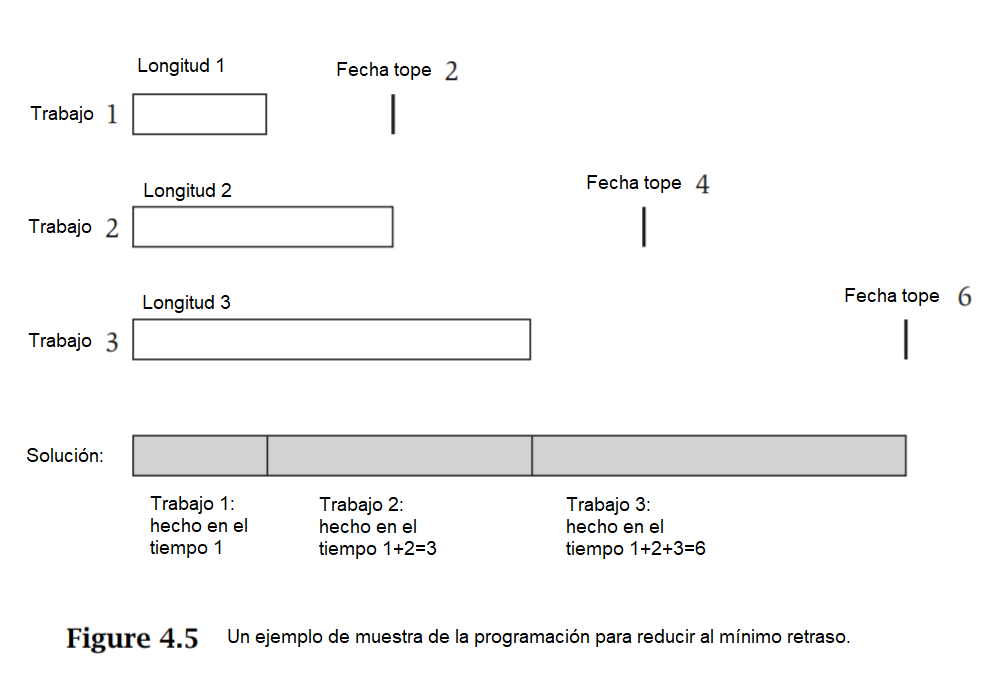
\includegraphics[scale=0.5]{Imagenes-Seccion4/Fig_4_5.PNG}
\end{figure}


Decimos que una solicitud $i$ llega tarde si falta a la fecha límite, es decir, si $f(i)>d_i$. La tardanza de tal solicitud $i$ se define como $l_i = f (i) - d_i$. Diremos que $l_i = 0$ si la solicitud no es tardía. El objetivo en nuestro nuevo problema de optimización será planificar todas las solicitudes, utilizando intervalos no superpuestos, a fin de minimizar la tardanza máxima, $L = max_i$ $l_i$. Este problema surge naturalmente al planificar trabajos que necesitan usar una sola máquina, por lo que nos referiremos a nuestras solicitudes como trabajos.\\

La Figura 4.5 muestra una instancia de este problema, que consta de tres trabajos: el primero tiene una longitud $t_1 = 1$ y una fecha límite $d_1 = 2$; el segundo tiene $t_2 = 2$ y $d_2 = 4$; y el tercero tiene $t_3 = 3$ y $d_3 = 6$. No es difícil comprobar que la planificación de los trabajos en el orden $1$, $2$, $3$ conlleva una tardanza máxima de $0$.\\

\subsubsection*{Diseñando el Algoritmo}
¿Cómo se vería un algoritmo ávido para este problema? Hay varios enfoques ávidos naturales en los que observamos los datos $(t_i, d_i)$ sobre los trabajos y usamos esto para ordenarlos de acuerdo a una regla simple.\\

\begin{itemize}
\item Un enfoque sería planificar los trabajos en orden de aumentar la duración $t_i$, a fin de apartar rápidamente los trabajos cortos. Esto se ve inmediatamente muy simplista, ya que ignora por completo los plazos de los trabajos. Y, de hecho, considere una instancia de dos trabajos donde el primer trabajo tiene $t_1 = 1$ y $d_1 = 100$, mientras que el segundo trabajo tiene $t_2 = 10$ y $d_2 = 10$. Entonces, el segundo trabajo debe comenzarse de inmediato si queremos alcanzar la tardanza $L=0$, y planificar primero el segundo trabajo es la solución óptima.\\
\end{itemize}

\begin{itemize}
\item El ejemplo anterior sugiere que deberíamos preocuparnos por los trabajos cuyo tiempo de holgura $d_i-t_i$ disponible es muy pequeño; son los que deben iniciarse con la mínima demora. Por lo tanto, un algoritmo ávido más natural sería ordenar los trabajos para aumentar el margen de holgura  $d_i-t_i$. Desafortunadamente, esta regla ávida también falla. Considere una instancia de dos trabajos donde el primer trabajo tiene $t_1 = 1$ y $d_1 = 2$, mientras que el segundo trabajo tiene $t_2 = 10$ y $d_2 = 10$. Ordenar por aumentar la holgura colocaría el segundo trabajo primero en el cronograma, y el primer trabajo lo incurrirá en un retraso de $9$. (Termina en el momento 11, nueve unidades más allá de su fecha límite). Por otro lado, si planificamos primero el primer trabajo, entonces termina a tiempo y el segundo trabajo incurre en un retraso de solo $1$.\\
\end{itemize}


Sin embargo, existe un algoritmo ávido igualmente básico que siempre produce una solución óptima. Simplemente ordenamos los trabajos en orden creciente de sus plazos $d_i$, y los planificamos en este orden. (Esta regla a menudo se denomina Primero plazo más temprano). Hay una base intuitiva para esta regla: debemos asegurarnos de que los trabajos con plazos más tempranos se completen antes. Al mismo tiempo, es un poco difícil de creer que este algoritmo siempre produzca soluciones óptimás, específicamente porque nunca mira la longitud de los trabajos. Antes éramos escépticos del enfoque que ordenaba por longitud con el argumento de que arrojó la mitad de los datos de entrada (es decir, los plazos); pero ahora estamos considerando una solución que descarta la otra mitad de los datos. Sin embargo, Earliest Deadline First produce soluciones óptimás, y ahora demostraremos esto.\\

Primero especificamos alguna notación que será útil para hablar sobre el algoritmo. Al cambiar el nombre de los trabajos si es necesario, podemos asumir que los trabajos están etiquetados en el orden de sus fechas límite, es decir, tenemos: $d_1 ≤ ... ≤ d_n$. Simplemente planificaremos todos los trabajos en este orden. Nuevamente, sea $s$ la hora de inicio de todos los trabajos. La tarea 1 comenzará en el momento $s = s (1)$ y finalizará en el tiempo $f (1) = s (1) + t_1$; El trabajo 2 comenzará en el tiempo $s (2) = f (1)$ y finalizará en el tiempo $f (2) = s (2) + t_2$; Etcétera. Utilizaremos $f$ para indicar el tiempo de finalización del último trabajo programado. Escribimos este algoritmo aquí.\\

\begin{lstlisting}
 Ordene los trabajos en orden de sus fechas limite
 Supongamos por simplicidad de notacion que d1 <= ... <= dn
 Inicialmente, f = s
 Considere los trabajos i = 1,. . . , n en este orden
    Asignar trabajo i al intervalo de tiempo de s (i) = f a f (i) = f + ti
    Sea f = f + ti
 Fin
 Devuelve el conjunto de intervalos programados [s (i), f (i)] para i = 1,. . . , n
\end{lstlisting}

\subsubsection*{Analizando el algoritmo}
Para razonar acerca de la optimalidad del algoritmo, primero observamos que el cronograma que produce no tiene " espacios vacíos " -tiempos cuando la máquina no está funcionando pero todavía hay trabajos pendientes. El tiempo que transcurre durante un intervalo se denomina tiempo de inactividad: hay trabajo por hacer, pero por alguna razón la máquina está inactiva. La planificación producida por nuestro algoritmo no solo no tiene tiempo de inactividad; también es muy fácil ver que hay un horario óptimo con esta propiedad. No escribiremos una prueba para esto.\\

\textbf{(4.7)} Existe un horario óptimo sin tiempo de inactividad.\\

Ahora, ¿cómo podemos demostrar que nuestro horario $A$ es óptimo, es decir, su retraso máximo $L$ es lo más pequeño posible? Como en análisis previos, comenzaremos considerando un horario $O$ óptimo. Nuestro plan aquí es modificar gradualmente $O$, preservando su optimalidad en cada paso, pero eventualmente transformándolo en un horario que es idéntico al programa $A$ encontrado por el algoritmo ávido. Nos referimos a este tipo de análisis como un argumento de intercambio, y veremos que es una forma poderosa de pensar algoritmos ávidos en general.\\

Primero tratamos de caracterizar los horarios de la siguiente manera. Decimos que un cronograma $A$ tiene una inversión si un trabajo $i$ con fecha límite $d_i$ está planificado antes de otro trabajo $j$ con fecha límite anterior $d_j<d_i$. Tenga en cuenta que, por definición, la planificación $A$ producida por nuestro algoritmo no tiene inversiones. Si hay trabajos con plazos idénticos, puede haber muchos horarios diferentes sin inversiones. Sin embargo, podemos demostrar que todas estas planificaciones tienen el mismo retraso máximo $L$.\\

\textbf{(4.8) }Todas las planificaciones sin inversiones y sin tiempo de inactividad tienen la misma demora máxima.\\

\textbf{Demostración}. Si dos planificaciones diferentes no tienen inversiones ni tiempo de inactividad, es posible que no produzcan exactamente el mismo orden de trabajos, pero solo pueden diferir en el orden en que se planifican los trabajos con plazos idénticos. Considere tal plazo $d$. En ambos horarios, los trabajos con fecha límite $d$ se planifican consecutivamente (después de todos los trabajos con fechas límite más tempranas y antes de todos los trabajos con fechas límite posteriores). Entre los trabajos con fecha límite $d$, el último tiene la mayor tardanza, y esta tardanza no depende del orden de los trabajos.  $\blacksquare$\\

El principal paso para mostrar la optimalidad de nuestro algoritmo es establecer que existe un cronograma óptimo que no tiene inversiones ni tiempo de inactividad. Para hacer esto, comenzaremos con cualquier horario óptimo que no tenga tiempo de inactividad; luego lo convertiremos en un cronograma sin inversiones sin aumentar su retraso máximo. Por lo tanto, la planificación resultante después de esta conversión también será óptima.\\

\colorbox{mygray}{\parbox{15cm}{
	\textbf{(4.9)}  Existe un horario óptimo que no tiene inversiones ni tiempo de inactividad.}}\\\\


\textbf{Demostración}. Por (4.7), hay un horario óptimo $O$ sin tiempo de inactividad. La prueba consistirá en una secuencia de enunciados. El primero de estos es simple de establecer.\\

\begin{enumerate}
\item  \textit{Si $O$ tiene una inversión, entonces hay un par de trabajos $i$ y $j$ tales que $j$ está planificado inmediatamente después de $i$ y tiene $d_j$ <$d_i$.\\}

De hecho, considere una inversión en la que un trabajo a está planificado en algún momento antes del trabajo $b$, y $d_a$> $d_b$. Si avanzamos en el orden planificado de trabajos de $a$ a $b$ uno por vez, tiene que llegar un punto en el que la fecha límite que vemos disminuya por primera vez. Esto corresponde a un par de trabajos consecutivos que forman una inversión.\\

Ahora supongamos que $O$ tiene al menos una inversión, y por (1), supongamos que $i$ y $j$ son un par de solicitudes invertidas que son consecutivas en el orden planificado. Disminuiremos el número de inversiones en $O$ al intercambiar las solicitudes $i$ y $j$ en la planificación $O$. El par $(i,j)$ formó una inversión en $O$, esta inversión es eliminada por el intercambio y no se crean nuevas inversiones. Así tenemos:
\item  \textit{Después de intercambiar $i$ y $j$ obtenemos un cronograma con una inversión menos.}\\

La parte más difícil de esta prueba es argumentar que el horario invertido también es óptimo.

\item  \textit{El nuevo horario intercambiado tiene un retraso máximo no mayor que el de $O$.}\\

Está claro que si podemos probar (3), entonces hemos terminado. La planificación inicial $O$ puede tener como máximo $\binom{n}{2}$ inversiones (si todos los pares están invertidos) y, por lo tanto, después de un máximo de $\binom{n}{2}$ intercambios obtenemos un cronograma óptimo sin inversiones.\\Así que ahora concluimos demostrando (3), mostrando que al intercambiar un par de trabajos invertidos consecutivos, no aumentamos el retraso máximo $L$ de la planificación.  $\blacksquare$\\
\end{enumerate}

\textbf{Prueba de (3)}. Inventamos alguna notación para describir el programa $O$: supongamos que cada solicitud $r$ está programada para el intervalo de tiempo $[s(r), f(r)]$ y tiene retraso $l'_r$. Sea $L' = max_r$ $l'_r $ denote la máxima latencia de este cronograma. Sea $\overline{O}$ el horario intercambiado; utilizaremos $\overline{s} (r)$, $\overline{f} (r)$,$\overline{f}_r$ y$\overline{L}$ para indicar las cantidades correspondientes en el programa intercambiado.\\

\begin{figure}[h]
\centering
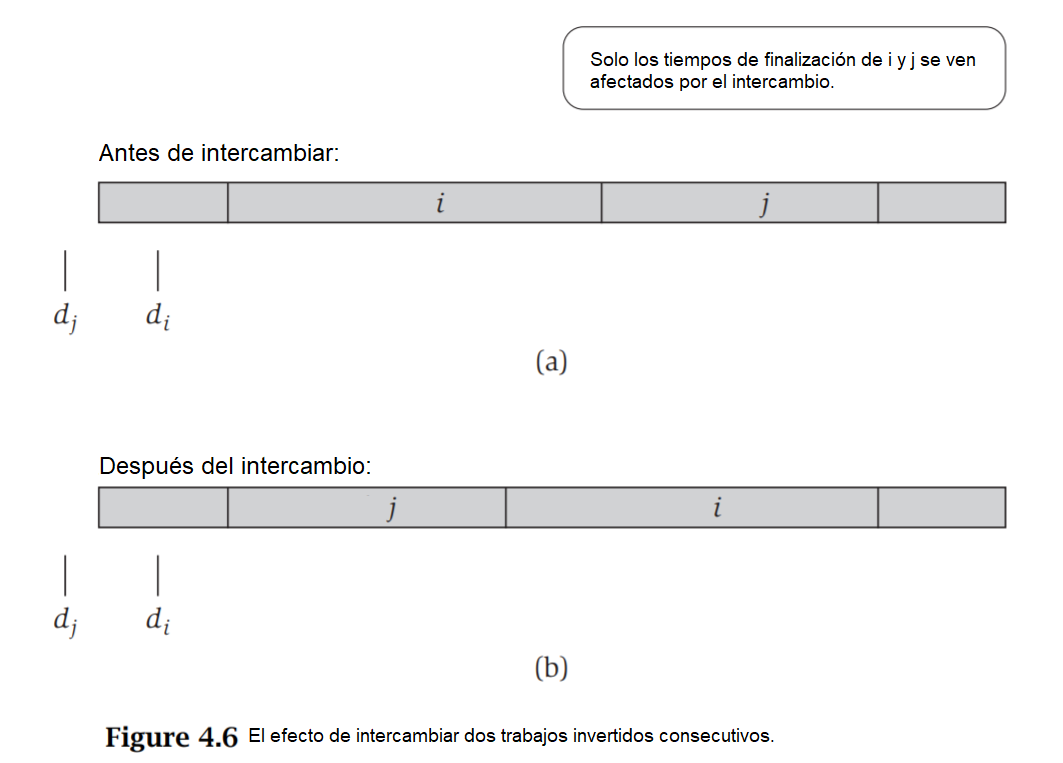
\includegraphics[scale=0.5]{Imagenes-Seccion4/Fig_4_6.PNG}
\end{figure}
Ahora recuerda nuestros dos trabajos invertidos adyacentes $i$ y $j$. La situación es más o menos como se muestra en la Figura 4.6. El tiempo de finalización de $j$ antes del intercambio es exactamente igual al tiempo de finalización de $i$ después del intercambio. Por lo tanto, todos los trabajos distintos $i$ y $j$ terminan al mismo tiempo en los dos programás. Además, el trabajo $j$ se terminará más temprano en el nuevo cronograma y, por lo tanto, el intercambio no aumentará la latencia del trabajo $j$.\\

Por lo tanto, lo único de lo que debemos preocuparnos es el trabajo $i$: su latencia puede haberse incrementado, y ¿qué pasa si esto realmente aumenta la latencia máxima de todo el cronograma? Después del intercambio, el trabajo termina en el momento $f(j)$, cuando el trabajo $j$ finalizó en el programa $O$. Si el trabajo $i$ se retrasa en este nuevo cronograma, su retraso es $\overline{l}_i = \overline{f}(i) - d_i = f (j) - d_i$. Pero el punto crucial es que $i$ no puede estar más tarde en el horario $\overline{O}$ que $j$ estaba en el horario $O$. Específicamente, nuestra suposición $d_i > d_j$ implica que:\\$\overline{l}_i =f(j)- d_i <f(j)-d_j= l'_j$.\\
Como la latencia del programa $O$ era $L' ≥ l'_j> \overline{l}_i$, esto muestra que el intercambio no aumenta la latencia máxima del programa.  $\blacksquare$\\

La optimalidad de nuestro algoritmo ávido ahora sigue inmediatamente.\\

\textbf{(4.10)} El programa $A$ producido por el algoritmo ávido tiene un retraso máximo óptimo $L$.\\

\textbf{Demostración}. El enunciado (4.9) demuestra que existe un cronograma óptimo sin inversiones. Ahora, por (4.8) todos los programás sin inversiones tienen la misma latencia máxima, por lo que el cronograma obtenido por el algoritmo ávido es óptimo.\\

\subsubsection*{Extensiones:}
Hay muchas generalizaciones posibles de este problema de programación. Por ejemplo, asumimos que todos los trabajos estaban disponibles para comenzar en la hora de inicio común $s$. Una versión natural, pero más dura, de este problema contendría solicitudes que, además de la fecha límite $d_i$ y la hora solicitada $t_i$, también tendrían un tiempo de inicio $r_i$ más temprano posible. Este tiempo de inicio posible más temprano se conoce generalmente como el tiempo de liberación. Los problemás con los tiempos de liberación surgen naturalmente en los problemás de programación donde las solicitudes pueden tomar la forma: ¿ Puedo reservar la sala para una conferencia de dos horas, en algún momento entre la 1 P.M. y 5 P.M.? Nuestra prueba de que el algoritmo ávido encuentra una solución óptima se basó fundamentalmente en el hecho de que todos los trabajos estaban disponibles en la hora de inicio común. (¿ Ves dónde ?) Desafortunadamente, como veremos más adelante en el libro, en el Capítulo 8, esta versión más general del problema es mucho más difícil de resolver de manera óptima.\\




\subsection{Caminos más cortos en un grafo}
Algunos de los algoritmos básicos para grafos están basados en principios del diseño de algoritmos ávidos. Aquí aplicamos un algoritmo ávido en el problema de encontrar los caminos más cortos, y en la siguiente sección veremos la construcción de árboles recubridores de mínimo costo.\\\\

\textbf{El problema}
Como hemos visto, los grafos son típicamente usados para modelar redes en las cuales uno va de un punto al otro -  atravesando una secuencia de caminos, o atravesando una secuencia de nodos de comunicación por rutas intermedias. Como resultado, un básico problema algorítmico consiste en determinar el menor camino entre nodos en un grafo. Podríamos plantear esto como una pregunta “punto a punto” : Dados los nodos $u$ y $v$, ¿Cuál es el mínimo camino entre $u$ y $v$? O podríamos pedir más información: Dado un nodo inicial $s$, ¿ Cuál es el camino más corto de $s$ a cada otro nodo?\\

En concreto el problema de los caminos más cortos es el siguiente. Tenemos un grafo dirigido $G=(V,E)$, con un determinado nodo de inicio $s$. Asumimos que s tiene un camino a cada otro nodo en $G$. Cada arista $e$ tiene longitud $l_e$ >=  0 indicando el tiempo (o distancia, costo, etc.) que toma atravesar $e$. Para un camino $P$, la longitud de $P$ – denotada $l(P)$ – es la suma de las longitudes de todas las aristas de $P$. Nuestro objetivo es determinar el camino más corto de $s$ a cualquier otro nodo en el grafo. Nótese que aunque el problema fue especificado para un grafo dirigido, podemos manejar el caso de un grafo no dirigido simplemente reemplazando cada arista no dirigida $e=(u,v)$ de longitud $l_e$ por dos aristas dirigidas $(u,v)$ y $(v,u)$, cada una de largo $l_e$.\\\\

\subsubsection*{Diseñando el algoritmo}
En 1959, Edsger Dijkstra propuso un simple algoritmo ávido para resolver el problema de los caminos más cortos. Comenzamos describiendo un algoritmo que solo determina el largo del camino más corto de $s$ a cualquier otro nodo en el grafo; es entonces fácil obtener los caminos también. El algoritmo mantiene un conjunto $S$ de vértices $u$ para los cuales hemos determinado una distancia, $d(u)$, del camino más corto desde $s$; esta es la parte “explorada” del grafo. Inicialmente $S={s}$, y $d(s)=0$. Ahora, para cada nodo $v$ \(\in\) $V-S$, determinamos el camino más corto que puede ser construido pasando a través de un camino de la parte explorada $S$ hasta $u$ \(\in\) $S$, seguido por una única arista $(u,v)$. Esto es, consideramos la cantidad $d’(v)$ = min\{$d (u)$ + $l_e$ : $e=(u,w)$, $u$ \(\in\) $S$ \} . Elegimos el nodo $v$ \(\in\) $V-S$ para el cual esta distancia es la mínima, añadimos $v$ a $S$, y definimos $d(v)$ como el valor de $d’(v)$.\\

\begin{lstlisting}
 Algoritmo Dijkstra (G,l)
Sea S el conjunto de nodos explorados
	Para cada u perteneciente a S, guardo la distancia d(u)
Inicialmente, S = {s} y d(s) = 0
While S != V
	Seleccionar un v no perteneciente a S con al menos un nodo de S
	para el cual d'(v) = min(d(u)+le ) es lo mas chico posible
	Agregar v a S y definir d(v)=d'(v)
EndWhile
\end{lstlisting}


Es simple producir los caminos $s-u$ correspondientes a las distancias encontradas
por el algoritmo de Dijkstra. Como cada nodo $v$ se agrega al conjunto $S$, simplemente registramos
la arista $(u, v)$ en la que se obtuvo el valor min\{$d (u)$ + $l_e$ : $e = (u, w)$, $u$ \(\in\) $S$ \} . El camino $P_v$ es implícitamente representado por estas aristas: si $(u,v)$ es la arista que guardamos para $v$, entonces $P_v$ es (recursivamente) el camino $P_u$ seguido por una sola arista $(u,v)$. En otras palabras, para construir $P_v$, simplemente empezamos en $v$, seguimos las aristas que guardamos en $u$ en orden inverso a su predecesor, y seguimos de esta forma hasta que alcanzamos $s$. Note que $s$ debe ser alcanzado, ya que nuestro camino hacia atrás desde $v$ visita nodos que fueron agregados a $S$ más y más temprano.\\

Para entender mejor lo que el algoritmo está haciendo, considere la representación de su ejecución en 4.7. En el instante que representa la imagen, se han realizado 2 iteraciones: La primera agrego el nodo $u$, y la segunda el nodo $v$. En la iteración que le sigue, el nodo $x$ será añadido porque logra el menor valor de $d'(x)$; Gracias a la arista $(u,x)$, tenemos $d'(x)= d(u)$ + $l_{ux}$ = 2. Note que intentar añadir el nodo y o $z$ al conjunto $S$ en este punto causaría un valor incorrecto para las distancias de los caminos más cortos; eventualmente, estos nodos serán añadidos desde las aristas de $x$.\\

\begin{figure}[h]
\centering
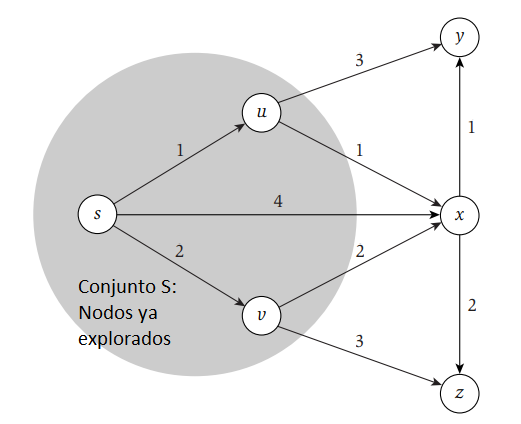
\includegraphics[scale=0.5]{Imagenes-Seccion4/fig_4_7.PNG}
\end{figure}
\textbf{Figura 4.7} Una muestra de la ejecución del algoritmo de Dijkstra. El siguiente nodo en ser añadido al conjunto $S$ será $x$, dado el camino por $u$.\\

\subsubsection*{Analizando el algoritmo}

Vemos en este ejemplo que el Algoritmo de Dijkstra está haciendo lo correcto y
evitando trampas recurrentes: hacer crecer el conjunto $S$ por el nodo incorrecto puede conducir a una
sobreestimacion de la distancia del camino más corto a ese nodo. La pregunta es:
¿Es siempre cierto que cuando el algoritmo de Dijkstra agrega un nodo $v$, obtenemos la verdadera
distancia más corta a $v$?\\
	Ahora respondemos esto probando la corrección del algoritmo, mostrando que los caminos $P_u$ realmente son los caminos más cortos. El algoritmo de Dijkstra es ávido en el sentido de que siempre forma el nuevo camino más corto $s-v$ que podemos formar de un camino en $S$ seguido de otra arista más. Probamos su corrección usando una variante de
nuestro primer estilo de análisis: mostramos que "se mantiene por delante" de todas las demás soluciones
estableciendo, inductivamente, que cada vez que selecciona un camino a un nodo $v$, ese
camino es más corto que cualquier otra ruta posible a $v$.\\\\

 \colorbox{mygray}{\parbox{15cm}{
	\textbf{(4.14)}  Considere el conjunto $S$ en un punto cualquiera durante la ejecución del algoritmo. Para cada $u$ \(\in\) $S$, el camino $P_u$ es el más corto de $s$ a $u$.}}\\\\

Tenga en cuenta que este hecho establece inmediatamente la corrección del Algoritmo, ya que podemos aplicarlo cuando el algoritmo finaliza, en el cual el punto $S$ incluye todos los nodos.\\

\textbf{Demostración}. Probamos esto por inducción en el tamaño de $S$. El caso $|S|=1$ es fácil, ya que tenemos $S$=\{s\} y $d(s)=0$. Supongamos que esto se mantiene cuando $|S|=k$ para algún valor de $k > 1$; Ahora aumentamos $S$ a $k+1$ añadiendo el nodo $v$.
Sea $(u,v)$ la ultima arista el el camino $s-v$, $P_v$.\\
Por hipótesis de inducción, $P_u$ es el camino más corto $s-u$ para cada $u$ \(\in\) S. Ahora considere cualquier otro camino $s-v$, denominado $P$; queremos mostrar que es al menos tan largo como $P_v$. Para alcanzar $v$, este camino debe salir de $S$ en alguna parte; sea y el primer nodo en $P$ que no está en $S$, y sea x \(\in\) $S$ el nodo justo antes de $y$.\\
	La situación es ahora como la descrita en la figura 4.8, y la clave de la prueba es simple: $P$ no puede ser más corto que $P_v$ porque ya es al menos tan largo como $P_v$ para cuando salió de $S$. 
De hecho, en la iteración $k + 1$, del
Algoritmo debe haber considerado agregar el nodo y al conjunto $S$ a través de la arista $(x, y)$
y rechazó esta opción a favor de agregar v. Esto significa que no hay camino
de $s$ a $y$ a través de $x$ que es más corto que $P_v$. Pero el subtrayecto de $P$ hasta y es
tal camino, y entonces este subtrayecto es al menos tan largo como $P_v$. Como las longitudes de arista
son no negativas, el camino completo $P$ es al menos tan largo como $P_v$ también.\\
Esta es una prueba completa; uno también puede expresar el argumento del párrafo anterior utilizando las siguientes desigualdades. Sea $P'$ el subcamino de $P$ desde $s$ hasta $x$. Ya que $x$ \(\in\) $S$, sabemos por hipótesis de inducción que $P_x$ es un camino más corto de $s-x$ (de largo $d(x)$), y entonces $l(P')$ \(\geq\) $l(P_x)=d(x)$. Entonces el subcamino de $P$ hasta el nodo $y$ tiene longitud $l(P')+l(x,y)$ \(\geq\) $d(x)+l(x,y)$ \(\geq\) $d'(y)$, y el camino completo $P$ es al menos tan largo como este subcamino. Finalmente, ya que el algoritmo selecciono $v$ en esta iteración, sabemos que $d'(y)$ \(\geq\) $d'(v)=l(P_v)$. Combinando estas desigualdades tenemos que $l(P)$ \(\geq\) $l(P') + l(x,y)$ \(\geq\) $l(P_v)$. \(\blacksquare\)\\

\begin{figure}[h]
\centering
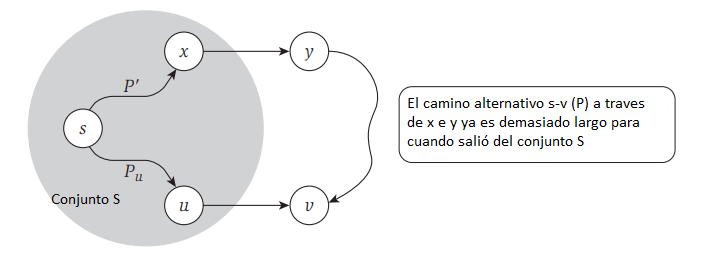
\includegraphics[scale=0.5]{Imagenes-Seccion4/fig_4_8.PNG}
\end{figure}
\textbf{Figura 4.8} El camino más corto $P_v$ y un camino alternativo $P$ de $s$ a $v$ a través del nodo $y$.\\


Aquí hay dos observaciones sobre el algoritmo de Dijkstra y su análisis. Primero, el algoritmo no siempre encuentra las rutas más cortas si alguna de las aristas puede tener longitudes negativas ( ¿ Ves dónde se rompe la prueba?) Muchas de las aplicaciones de camino más corto implican longitudes de arista negativas, y un algoritmo más complejo, de Bellman y Ford, se requiere para este caso. Veremos este algoritmo cuando consideremos el tema de la programación dinámica.\\


La segunda observación es que el algoritmo de Dijkstra es, en cierto sentido, incluso
más simple de lo que hemos descrito aquí. El algoritmo de Dijkstra es realmente una
versión "continua" del algoritmo BFS para atravesar un
grafo, y puede estar motivado por la siguiente intuición física. Suponga que
las aristas de $G$ forman un sistema de tuberías llenas de agua, unidas en
los nodos; cada arista $e$ tiene una longitud $l_e$ y un ancho fijo. Ahora
supongamos que una gota extra de agua cae en el nodo $s$ y comienza una onda desde $s$. Como
la ola se expande fuera de los nodos a una velocidad constante, la esfera en expansión
del frente de onda alcanza nodos en orden creciente de su distancia desde $s$. Es
fácil de creer (y también cierto) que el camino tomado por el frente de onda para llegar a
cualquier nodo v es la ruta más corta. De hecho, es fácil ver que esto es exactamente el
camino a v encontrado por el algoritmo de Dijkstra, y que los nodos son descubiertos por
la expansión del agua en el mismo orden en que fueron descubiertas por el algoritmo de Dijkstra.\\

\subsubsection*{Implementación y tiempo de ejecución} Para concluir nuestra discusión sobre
el algoritmo de Dijkstra, consideramos su tiempo de ejecución. Hay $n$ - 1 iteraciones del ciclo
While para un grafo con n nodos, ya que cada iteración agrega un nuevo nodo $v$
a $S$. Seleccionar el nodo correcto v de manera eficiente es un problema más sutil. Una primera impresión es que cada iteración debería considerar cada nodo $v  \in  S$,
y recorrer todas las aristas entre S y v para determinar el mínimo
$\min{d (u) + l_e : e = (u, w), u \in S }$, para poder seleccionar el nodo $v$ para el cual este mínimo es el más pequeño. Para un grafo con $m$ aristas, calcular todos estos mínimos
puede tomar tiempo $O(m)$, por lo que esto llevaría a una implementación que se ejecuta en tiempo
$O(mn)$.\\

Podemos mejorar considerablemente si utilizamos las estructuras de datos correctas. Primero nosotros
mantendremos explícitamente los valores de los mínimos $d(v) = \min{d (u) + l_e : e =(u,w), u \in  S }$  para cada nodo $v  \in  V - S$, en lugar de volver a calcularlos en cada iteración.
Podemos mejorar aún más la eficiencia al mantener los nodos $V - S$ en una cola de prioridad con 
$d'(v)$ como sus claves(prioridades). Las colas de prioridad se discutieron en el Capítulo 2;
son estructuras de datos diseñadas para mantener un conjunto de $n$ elementos, cada uno con una
prioridad asociada. Una cola de prioridad puede insertar y eliminar elementos, cambiar
la clave de un elemento, y extraer el elemento con la clave mínima en forma eficiente. Necesitaremos
la tercera y cuarta de las operaciones anteriores: \textit{ChangeKey} y \textit{ExtractMin}.


¿ Cómo implementamos el algoritmo de Dijkstra usando una cola de prioridad? Nosotros ponemos
los nodos $V$ en una cola de prioridad con $d'(v)$ como la clave para $v \in V$. Para seleccionar el nodo
$v$ que se debe agregar al conjunto $S$, necesitamos la operación \textit{ExtractMin}. Para ver
cómo actualizar las claves, considere una iteración en la cual el nodo $v$ se agrega a $S$, y
sea $w$ \(\notin\) $S$ un nodo que permanezca en la cola de prioridad.
¿Qué tenemos que hacer para actualizar el valor de $d'(w)$? Si $(v, w)$ no es una arista, entonces no tenemos que hacer
nada: el conjunto de aristas considerado en el mínimo min\{$d (u)$ + $l_e$ : $e=(u,w)$, $u$ \(\in\) $S$ \} 
es exactamente lo mismo antes y después de agregar $v$ a $S$. Si por otro lado, $e' = (v, w)  \in  E$, el nuevo valor para la clave es $min (d'(w), d (v) + l_{e'})$. Si $d'(w)> d (v) + l_{e'}$ entonces tenemos que usar la operación \textit{ChangeKey} para disminuir
la clave del nodo w apropiadamente. Esta operación \textit{ChangeKey} puede ocurrir como máximo
una vez por arista, cuando la cola de la arista $e'$ se agrega a $S$. En resumen, tenemos
el siguiente resultado.\\

 \colorbox{mygray}{\parbox{15cm}{
	\textbf{(4.14)}  Usando una cola de prioridad, el algoritmo de Dijkstra puede ser implementado en un grafo con $n$ nodos y $m$ aristas de forma tal que corra en tiempo $O(m)$, más el tiempo de n operaciones \textit{ExtractMin} y m operaciones \textit{ChangeKey}.}}\\
    
	Usando la implementación de la cola de prioridad basada en montículos que fue discutida en el capitulo 2, cada operación de la cola de prioridad puede correr en tiempo $O(logn)$. Entonces el tiempo total de la implementación es $O(m.logn)$.\\
    

\subsection{El problema del árbol de cubrimiento mínimo}

Ahora aplicamos un argumento de intercambio en el contexto de un segundo problema en los grafos: el problema del mínimo árbol de cubrimiento.\\

\textbf{El problema}\\

Supongamos que tenemos un conjunto de ubicaciones V = \{$v_1$, $v_2$, ..., $v_n$\}, y queremos construir una red de comunicación sobre ellas. Si la red fuese conexa debería haber un camino entre cada par de nodos. En caso de no serla, deseamos construirla de la forma más barata posible.\\
	Para ciertos pares ($v_i$, $v_j$), podemos construir un enlace directo entre $v_i$ y $v_j$ para
un cierto costo c($v_i$, $v_j$)> 0. Por lo tanto, podemos representar el conjunto de posibles enlaces que se puede construir usando un grafo G = $(V, E)$, con un costo positivo $C_e$ asociado con
cada arista $e$ = ($v_i$, $v_j$). El problema es encontrar un subconjunto de las aristas $T$ ⊆ $E$ para
que el grafo $(V,T)$ sea conexo, y el costo total \(\sum\) $c_e$ sea lo más pequeño posible. (Asumiremos que el grafo completo $G$ es conexo; de lo contrario, no hay solución posible).\\

Haremos la siguiente observación:\\
    
\textbf{(4.16)} Sea $T$ una solucion de mínimo costo al problema de diseño de conexión definido arriba. Entonces $(V,T)$ es un árbol.\\

\textbf{Demostración} Por definición, $(V,T)$ debe ser conexo; demostraremos que tampoco contendrá ciclos. Entonces, supongamos que contiene un ciclo $C$, y sea $e$ cualquier
arista en $C$. Afirmamos que ($V$, $T$ - \{$e$\}) todavía es conexo, ya que cualquier camino que haya pasado anteriormente por la arista $e$ ahora puede ir "para el otro lado" alrededor del resto
del ciclo $C$ en su lugar. Se deduce que ($V$, $T$ - \{$e$\}) también es una solución válida para el
problema, y es más barata, lo cual es una contradicción.\\

Si permitimos que algunas aristas tengan costo 0 (Esto es, asumimos solo que los costos $c_e$ son no negativos), entonces una solución de costo mínimo al problema de diseño de red puede tener aristas extra -  aristas que tienen 0 costo y podrían ser borradas opcionalmente. Pero incluso en este caso, siempre hay una solución con costo mínimo que es un árbol. Empezando de cualquier solución optima, podemos seguir borrando aristas de ciclos hasta obtener un árbol; con aristas de costo no negativo, y el costo no aumentaría en este proceso.\\
	
Llamaremos a un subconjunto $T$ ⊆ $E$ un árbol de cubrimiento de $G$ si $(V,T)$ es un árbol. La proposición (4.16) dice que el objetivo de nuestro problema de diseño de red puede ser redefinido como el de encontrar el árbol de cubrimiento más barato en un grafo; por esta razón, es llamado el \textit{problema del árbol de cubrimiento Mínimo}. A no ser que $G$ sea un grafo muy simple, este tendrá una cantidad exponencial de diferentes árboles de cubrimiento, cuyas estructuras pueden ser muy distintas una de otra. Entonces no es del todo claro como encontrar eficientemente el árbol más barato de entre todas estas opciones.\\
    
\subsubsection*{Diseñando Algoritmos}
Como en los problemás que hemos visto anteriormente, es fácil inventar un número de algoritmos greedy para el problema. Pero curiosamente, y por suerte, este es un caso en el cual muchos de los primeros algoritmos a los que uno se le ocurre son correctos: éstos resuelven el problema de forma optima. Procederemos a examinar algunos de estos algoritmos ahora para luego descubrir, mediante un par de argumentos de intercambio, algunas de las razones fundamentales para esta multitud de algoritmos simples y óptimos.\\

Aquí hay 3 algoritmos ávidos, cada uno de los cuales encuentra de forma correcta un árbol de cubrimiento mínimo.\\

\begin{itemize}

\item Un algoritmo simple comienza sin ninguna arista en absoluto y construye un árbol de cubrimiento al insertar sucesivamente las aristas de $E$ en orden de costo creciente. A medida que avanzamos por las aristas en este orden, insertamos cada arista $e$ siempre que no cree un ciclo cuando se agrega a las aristas que tenemos ya insertadas. Si, por otro lado, insertar $e$ daría como resultado un ciclo, entonces simplemente descartamos $e$ y continuamos. Este enfoque se llama Algoritmo de Kruskal.

\item Otro simple algoritmo greedy puede ser diseñado en analogía con el algoritmo de Dijkstra para caminos, aunque, de hecho es aun más fácil de especificar. Empezamos con un nodo raíz $s$ e intentamos de formar un árbol desde $s$ hacia afuera. en cada paso, simplemente agregamos el nodo que puede ser unido en la forma más barata al árbol parcial que ya tenemos. más concretamente mantenemos un conjunto $S$ ⊆ $V$ en el cual se ha construido un árbol de cubrimiento hasta ahora. Inicialmente, $S$=\{$s$\}. En cada iteración aumentamos $S$ por un nodo, agregando en nodo $v$ que minimiza el "costo de unión" min\{$c_e$ : $e=(u,w)$, $u$ \(\in\) $S$ \}, e incluimos la arista $e=(u,v)$ que logra este mínimo en el árbol de cubrimiento. Este método se llama algoritmo de Prim.

\item Finalmente, podemos diseñar un algoritmo greedy haciendo una versión "al revés" del algoritmo de Kruskal. Específicamente, empezamos con un grafo entero $(V,E)$ y empezamos a eliminar aristas en orden de costo decreciente. A medida que llegamos a cada arista $e$ (empezando de la más costosa), la borramos siempre que al hacerlo no desconectemos el grafo que tenemos actualmente. A falta de un mejor nombre, a este se le llama el algoritmo de eliminación inversa.
\end{itemize}

\begin{figure}[h]
\centering
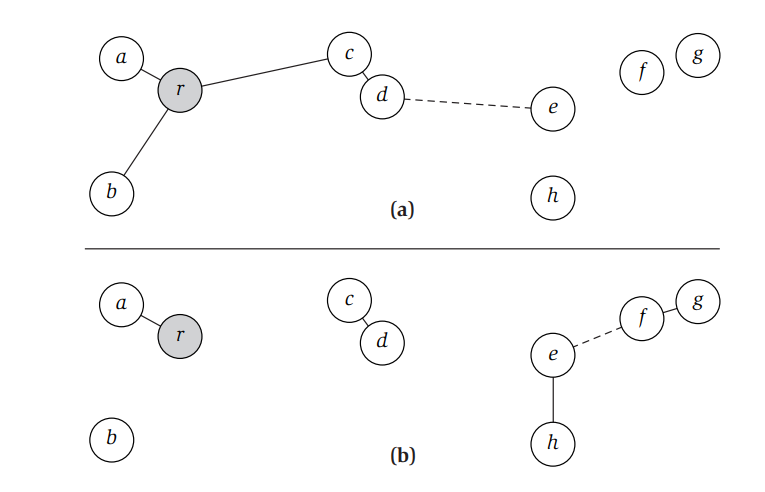
\includegraphics[scale=0.7]{Imagenes-Seccion4/fig_4_9.PNG}
\textbf{Figura 4.9} Ejecución de muestra de los algoritmos de árbol recubridor mínimo de (a) Prim y (b) Kruskal, con la misma entrada. Las primeras 4 aristas agregadas al árbol recubridor están indicadas por líneas continuas; la siguiente arista que se agregará es una línea punteada.
\end{figure}


Por ejemplo, la Figura 4.9 muestra las primeros cuatro aristas añadidas por los algoritmos de Prim y Kruskal respectivamente, en una instancia geométrica del problema del árbol recubridor mínimo en el cual el costo de cada arista es proporcional a la distancia geométrica en el plano.\\

El hecho de que cada uno de estos algoritmos garantiza una solución optima sugiere que hay una cierta "robustez" el el problema del árbol recubridor mínimo - hay muchas maneras de llegar a la respuesta. A continuación exploramos algunas de las razones por las cuales tantos algoritmos diferentes producen árboles de mínimo costo.\\

\subsubsection*{Analizando los Algoritmos}
Todos estos algoritmos funcionan insertando o borrando repetidamente las aristas de una
solución parcial. Entonces, para analizarlos, sería útil tener en cuenta algunos
datos básicos que dicen cuándo es "seguro" incluir una arista en el árbol recubridor mínimo, y cuando es seguro eliminar una arista considerando que no hay manera posible de que ella esté en el árbol recubridor mínimo. Para los propósitos de
el análisis, haremos la suposición simplificadora de que todos los costos de arista son
distintos entre sí (es decir, no hay dos iguales). Esta suposición hace más fácil expresar los argumentos que siguen, y vamos a mostrar más adelante en esta sección como estas suposiciones pueden ser eliminadas.\\

\textbf{¿ Cuando es seguro incluir una arista en el árbol recubridor mínimo?} El hecho crucial acerca de la inserción de aristas es la siguiente proposición, a la cual llamamos propiedad de corte.\\

\colorbox{mygray}{\parbox{15cm}{
\textbf{(4.17)}  Suponga que todos los costos de aristas son distintos. Sea $S$ cualquier subconjunto de nodos que no es ni vacío ni igual al V entero, y sea la arista $e=(v,w)$ la de mínimo costo con un nodo en $V$ y el otro en $V-S$. Entonces todo árbol recubridor mínimo contiene a la arista $e$.}}\\\\

\textbf{Demostración} Sea $T$ un árbol recubridor  que no contiene a $e$; necesitamos probar que $T$ no tiene el costo mínimo posible. Haremos esto usando un argumento de intercambio: Identificaremos una arista $e'$ en $T$ que sea más costosa que $e$, y por propiedad cambiar $e$ por $e'$ resulta en otro albor recubridor. Este árbol recubridor resultante será entonces más barato que $T$, como queríamos.\\

La clave es entonces encontrar una arista que pueda ser cambiada por $e$. Recordar que las puntas de $e$ son $v$ y $w$. $T$ es un árbol recubridor, entonces debe haber un amino $P$ en $T$ desde $v$ hasta $w$. Empezando de v, suponga que seguimos los nodos de $P$ en una secuencia; hay un primer nodo $w'$ en $P$ que está en $V-S$. Sea $v'$ \(\in\) $S$ el nodo justo antes que $w'$ en $P$, y sea $e'=(v',w')$ la arista uniéndolos. Entonces, e' es una arista de T con una punta en $S$ y la otra en $V-S$. La situación en esta parte de la prueba se puede ver en la figura 4.10.\\

Si cambiamos $e$ por $e'$, obtenemos un conjuntos de aristas $T'=T-$\{$e'$\}\(\cup\)$\{e\}$. Decimos que $T'$ es un árbol recubridor. Claramente $(V,T')$ es conexo, ya que $(V,T)$ es conexo, y cualquier camino en $(V,T)$ que use la arista $e'=(v',w')$ puede ahora ser redirigida en $(V,T')$ para seguir la porción de $P$ desde $v'$ hasta $v$, luego la arista $e$, y luego la porción de w a $w'$. Para ver que $(V,T')$ también es acíclico, notar que el único ciclo en (V,T'\(\cup\)\{e'\}) es el que está compuesto por $e$ y el camino $P$, y este ciclo no está presente en $(V,T')$ dado que $e'$ fue borrado.\\

Mencionamos arriba que la arista $e'$ tiene un extremo en $S$ y la otra en $V-S$. Pero $e$ es la arista menos costosa con esta propiedad, entonces $c_e$ < $c_{e'}$. (La desigualdad es estricta ya que no hay 2 aristas con el mismo costo.) Entonces el costo total de $T'$ es menor que el de $T$, como queríamos. \(\blacksquare\)\\
    
\begin{figure}[h]
\centering
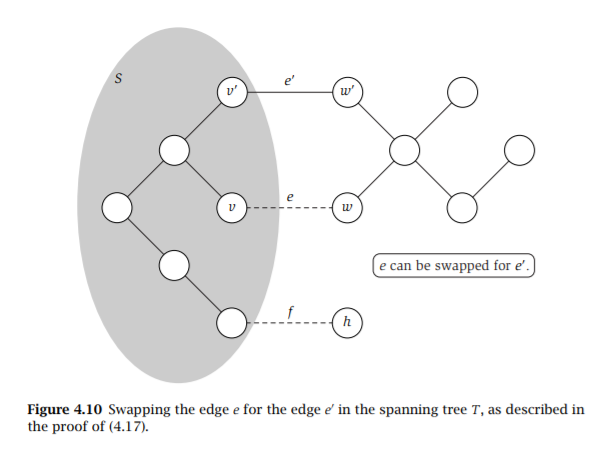
\includegraphics[scale=0.8]{Imagenes-Seccion4/fig4_10.PNG}
\textbf{Figura 4.10} Cambiar la arista e por la arista e' en el árbol recubridor T, según se describe en la prueba de (4.17).
\end{figure}
    
La prueba de (4.17) es un poco más sutil de lo que parece al principio. Para apreciar esta sutileza, considere el siguiente argumento, que es más corto pero incorrecto para probar (4.17). Sea $T$ un árbol recubridor que no contiene a $e$. Ya que $T$ es un árbol recubridor, debe tener una arista $f$ con una punta en $S$ y la otra en $V-S$. Como $e$ es la arista más barata con esta propiedad, tenemos que $c_e$ < $c_f$, y entonces $T$-\{$f$\}\(\cup\)\{$e$\} es un árbol recubridor que es más barato que $T$.\\

El problema con este argumento no yace en el hecho de que $f$ exista, o que $T$-\{$f$\}\(\cup\)\{$e$\} es más barato que $T$. La dificultad es que $T$-\{$f$\}\(\cup\)\{$e$\} puede no ser un árbol recubridor, como se puede apreciar en la figura 4.10. El punto es que no podemos probar (4.17) simplemente eligiendo cualquier arista en $T$ que cruce de $S$ a $V-S$; hay que tener cuidado al elegir la adecuada.\\
    
\textbf{La optimalidad de los algoritmos de Kruskal y Prim} Ahora podemos probar fácilmente la optimalidad de los algoritmos de Kruskal y Prim. El punto es que ambos algoritmos solo incluyen una arista cuando esta justificado por la propiedad de corte (4.17).\\

\colorbox{mygray}{\parbox{15cm}{
\textbf{(4.18)}  El algoritmo de Kruskal produce un árbol de cubrimiento mínimo de $G$.}}\\\\

\textbf{Demostración} Considere cualquier arista $e=(v,w)$ añadida por el algoritmo de Kruskal, y se $S$ el conjunto de todos los nodos a los cuales $v$ tiene un camino en el momento justo anterior de añadir $e$. Claramente $v$ \(\in\) $S$, pero $w$ \(\notin\) $S$, ya que al agregar $e$ no se crea un ciclo. Por otra parte, no se ha encontrado ninguna arista de $S$ a $V-S$, ya que cualquiera de esas aristas podría haber sido agregada sin crear un ciclo, y por lo tanto hubiera sido agregado por el algoritmo de Kruskal. Por lo tanto, $e$ es la arista más barata con un extremo en $S$ y el otro en $V-S$, y así por (4.17) pertenece a cada árbol recubridor mínimo.\\

Entonces si podemos mostrar que la salida $(V,T)$ del algoritmo de Kruskal es de hecho un árbol recubridor de $G$, entonces habremos terminado. Claramente $(V,T)$ no contiene ciclos, ya que el algoritmo está explicita mente diseñado para evitar crear ciclos. Es más, si $(V,T)$ fuera no conexo, entonces existiría un conjunto no vacío de nodos $S$ (no igual a todo $V$) tal que no haya arista de $S$ a $V-S$. Pero esto contradice el comportamiento del algoritmo: sabemos que ya que $G$ es conexo, hay al menos una arista entre $S$ y $V-S$, y el algoritmo agregará la primera de estas que encuentre. \(\blacksquare\)\\

\colorbox{mygray}{\parbox{15cm}{
\textbf{(4.19)}  El algoritmo de Prim produce un árbol de cubrimiento mínimo de G.}}\\\\

\textbf{Demostración} Para el algoritmo de Prim, es también muy fácil probar que solo añade aristas que pertenecen a un árbol de cubrimiento mínimo. De hecho, en cada iteración del algoritmo, hay un conjunto $S$ \(\subseteq\) $V$ en el cual un árbol de cubrimiento parcial ha sido construido, y un nodo $v$ y arista $e$ se agregar para minimizar la cantidad min\{$c_e$ : $e = (u, w)$, $u$ \(\in\) $S$ \}. Por definición, $e$ es la arista más barata con un extremo en $S$ y el otro en $V-S$, y entonces por la propiedad de Corte (4.17) está en todo árbol recubridor mínimo.\\

Es también sencillo mostrar que el algoritmo de Prim produce un árbol recubridor de $G$, por lo cual produce uno mínimo. \(\blacksquare\)\\
    
\textbf{¿ Cuándo podemos garantizar que una arista no está en el árbol recubridor mínimo?} El hecho crucial sobre la eliminación de aristas es la siguiente proposición, a la cual llamaremos la Propiedad de Ciclo.\\
    
\colorbox{mygray}{\parbox{15cm}{
\textbf{(4.20)}  Asuma que todos los costos de arista son distintos. Sea $C$ un ciclo cualquiera en $G$, y sea $e=(v,w)$ la arista más cara perteneciente a $C$. Entonces $e$ no pertenece a ningún árbol recubridor mínimo de $G$.}}\\\\

\textbf{Demostración} Sea $T$ un árbol recubridor que contiene a $e$; necesitamos mostrar que $T$ no tiene el menor costo posible. Por analogía con la prueba de la propiedad de corte (4.17), haremos esto con un argumento de intercambio, cambiando $e$ por una arista más barata de tal manera que sigamos teniendo un árbol recubridor.\\

Entonces la pregunta es nuevamente: ¿ Cómo encontramos una arista más barata que puede ser cambiada de esta manera por $e$? Comencemos por borrar la arista $e$ de $T$; esto divide los nodos en dos componentes: $S$, que contiene al nodos $v$; y $V-S$, que contiene al nodo $w$. Ahora, la arista que utilizaremos en lugar de $e$ debe tener un extremo en $S$ y el otro en $V-S$, para poder conectarse al resto.\\
    
Podemos encontrar tal arista siguiendo el ciclo $C$. Las aristas de $C$ que no sean $e$ forman, por definición, un camino $P$  con un extremo en $v$ y el otro en $w$. Si seguimos $P$ desde $v$ hasta $w$, empezamos en $S$ y terminamos en $V-S$, entonces hay algún arista $e$' en $P$ que cruza de $S$ a $V-S$. Ver en figura 4.11 la ilustración de esto.\\

Ahora considere el conjunto de aristas $T'$=$T$-\{$e$\}\(\cup\)\{$e'$\}. Argumentando como en la prueba de la propiedad de corte (4.17), el grafo $(V,T')$ es conexo y no tiene ciclos, entonces $T$' es una árbol recubridor de $G$. Además, ya que $e$ es la arista más cara en $C$, y $e'$ pertenece a $C$, debe cumplirse que $e'$ es más barata que $e$, y entonces $T'$ es más barato que $T$, como queríamos probar. \(\blacksquare\)\\
    
\begin{figure}[h]
\centering
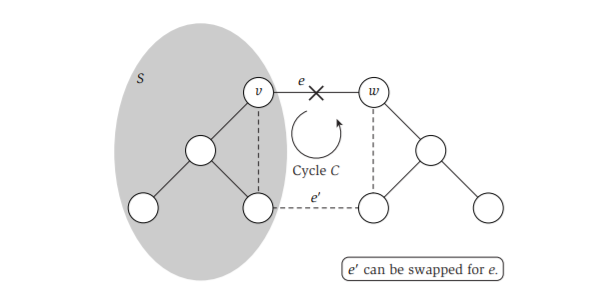
\includegraphics[scale=0.9]{Imagenes-Seccion4/fig4_11.PNG}
\textbf{Figura 4.11} Cambiar la arista $e'$ por la arista $e$ en el árbol recubridor $T$, como se describe en la prueba de (4.20).
\end{figure}

\textbf{\textit{Optimalidad del algoritmo de eliminación hacia atrás}} Ahora que tenemos la propiedad de ciclo (4.20), es fácil probar que el algoritmo de borrado hacia atrás produce un árbol recubridor mínimo. La idea básica es análoga a las pruebas de optimalidad de los dos algoritmos anteriores: borrar hacia atrás solo agrega una arista cuando está justificado por (4.20).\\

\colorbox{mygray}{\parbox{15cm}{
\textbf{(4.21)}  El algoritmo de borrado hacia atrás produce un árbol de cubrimiento mínimo de G.}}\\\\

\textbf{Prueba.} Considere cualquier arista $e=(v,w)$ eliminada por el algoritmo. En el momento de ser eliminada, $e$ está en un ciclo $C$; y como es la primer arista encontrada por el algoritmo en orden decreciente de costos, debe ser la más cara en $C$. Entonces por (4.20), $e$ no pertenece a ningún árbol recubridor mínimo.\\

Entonces si mostramos que la salida $(V,T)$ es un árbol recubridor de $G$, habremos terminado. Claramente $(V,T)$ es conexo, ya que algoritmo nunca elimina una arista cuando esta desconecta el grafo. Ahora suponga por absurdo que $(V,T)$ contiene un ciclo $C$. Considere la arista más cara $e$ de $C$, la cual sería la primera encontrada por el algoritmo. Esta arista debería haber sido eliminada, ya que esto no desconectaría el grafo, lo cual contradice el comportamiento del algoritmo.\(\blacksquare\)\\
    
Aunque no exploraremos esto más en detalle, la combinación de la propiedad de corte (4.17) y la propiedad de ciclo (4.20) implica que algo aun más general está pasando. \textit{Cualquier} algoritmo que construya un árbol recubridor mediante el agregado repetitivo de aristas cuando está justificado por la propiedad de corte y borre aristas cuando está justificado por la propiedad de ciclo -en cualquier orden- terminará construyendo un árbol recubridor mínimo. Este principio permite a uno diseñar algoritmos ávidos naturales para este problema más allá del árbol que consideramos aquí, y provee una explicación de por que tantos algoritmos ávidos producen una solución óptima a este problema.\\
    
Eliminar la suposición de que todos los costos perimetrales son distintos Hasta ahora, hemos supuesto que todos los costos de arista son distintos, y esta suposición ha hecho que el análisis sea más limpio en varios lugares. Ahora, supongamos que se nos da una instancia del Problema del árbol de expansión mínimo en el que ciertas arista tienen el mismo costo: ¿cómo podemos concluir que los algoritmos que hemos estado discutiendo aún ofrecen soluciones óptimas?\\

Resulta ser una manera fácil de hacer esto: simplemente tomamos la instancia y perturbamos todos los costos de arista por diferentes números extremadamente pequeños, para que todos se vuelvan distintos. Ahora, los dos costos que difirieron originalmente seguirán teniendo el mismo orden relativo, ya que las perturbaciones son muy pequeñas; y dado que todos nuestros algoritmos se basan solo en la comparación de los costos de las arista, las perturbaciones sirven simplemente como "desempate" para resolver comparaciones entre costos que solían ser iguales.\\

Además, afirmamos que cualquier árbol de expansión mínimo $T$ para la nueva instancia perturbada también debe haber sido un árbol de expansión mínimo para la instancia original. Para ver esto, observamos que si $T$ cuesta más que algún árbol $T*$ en la instancia original, entonces para perturbaciones lo suficientemente pequeñas, el cambio en el costo de $T$ no puede ser suficiente para hacerlo mejor que $T*$ bajo los nuevos costos. Por lo tanto, si ejecutamos cualquiera de nuestros algoritmos de árbol de expansión mínimo, utilizando los costos perturbados para comparar las aristas, produciremos un árbol de expansión mínimo $T$ que también es óptimo para la instancia original.\\  
% * <mathias2b@gmail.com> 2018-09-18T14:55:47.750Z:
% 
% Revisar si siguen faltando páginas
% 
% ^.
\subsection{Implementando el algoritmo de Kruskal: La estructura de datos Unión-Busqueda}

Uno de los problemas más básicos de grafos es encontrar el conjunto de componentes. En el Capítulo 3 discutimos algoritmos de tiempo lineal usando BFS y DFS para encontrar los componentes conexos de un grafo.\\

En esta sección, consideramos el escenario en el cual un grafo evoluciona a través de la adición de aristas. Es decir, el grafo tiene una cantidad fija de nodos, pero crece en correr del tiempo al tener aristas que aparecen entre ciertos pares de nodos. Nuestro objetivo es mantener el conjunto de componentes conexas de un grafo a través de este proceso evolutivo. Cuando una arista es agregada al grafo, nosotros no queremos tener que computar nuevamente los componentes conexos desde cero. Más bien, vamos a desarrollar una estructura que la llamaremos la estructura Unión-Buscar, la cual va a guardar una representación de los componentes de una manera que soporte búsqueda y actualización rápida.\\

Esta es exactamente la estructura de datos necesaria para implementar el algoritmo de Kruskal eficientemente. Como cada arista $e=(v,w)$ es considerada, necesitamos encontrar eficientemente las identidades de los componentes conexos que contengan a $v$ y $w$, y por lo tanto la arista $e$ debe estar incluida; pero si los componentes son los mismos, entonces existe un camino $v-w$ en las aristas que ya se incluyeron, y entonces $e$ debe ser omitida. En el evento que e es incluida, la estructura de datos también debe soportar la unión eficiente de los componentes de $v$ y $w$ en un solo componente. \\

\textbf{El problema}

La estructura de datos Unión-Buscar nos permite mantener conjuntos disjuntos (tales como los componentes de un grafo) en el siguiente manera. Dado un nodo $u$, la operación Buscar(u) va a retornar el nombre del conjunto que contiene a $u$. Esta operación puede ser usada para verificar si dos nodos u y v están en el mismo conjunto, simplemente verificando si Buscar($u$) = Buscar($v$). Además la estructura de datos va a implementar una operación Unión($A$, $B$) para tomar dos conjuntos $A$ y $B$ y unirlos en un único conjunto.\\

Estas operaciones pueden ser usadas para mantener componentes conexos en un grafo evolutivo $G=(V,E)$ mientras las aristas se van agregando. Los conjuntos serán componentes conexas del grafo. Para un nodo $u$, la operación Buscar(u) va a retornar el nombre del componente que contiene a $u$. Si le agregamos una arista $(u,v)$ al grafo, entonces primero verificamos si $u$ y $v$ pertenecen a la misma componente conexa (probando si Buscar($u$) = Buscar($v$)). Si ellos no pertenecen, entonces Unión(Buscar($u$), Buscar($v$)) puede ser usado para unir las dos componentes en una solo. Es importante notar que la estructura de datos Unión-Buscar solo puede ser usada para mantener componentes de un grafo mientras agregamos aristas; no está diseñada para manejar los efectos de borrar una arista, que puede resultar en un componente dividido en dos.\\
    
En resumen, la estructura de datos Unión-Buscar va a soportar tres operaciones.

\begin{itemize}
\item HacerUniónBuscar($S$) para un conjunto $S$ va a retornar una estructura de datos Unión-Buscar del conjunto $S$ donde todos los elementos están en conjuntos separados. Esto corresponde, por ejemplo, al componente conexo de un grafo sin aristas. Nuestro objetivo va a ser implementar HacerUniónBuscar en tiempo $O(n)$ donde $n=|S|$.
\item Para un elemento $u$ $\in$ $S$, la operación Buscar($u$) va a retornar el nombre 	del conjunto que contiene a $u$. Nuestro objetivo va a ser implementar Buscar($u$) en tiempo $O(log n)$. Algunas implementaciones que hemos discutido van a tomar solamente tiempo $O(1)$ para esta operación.
\item Para dos conjuntos $A$ y $B$, la operación Unión($A$, $B$) va a cambiar estructura de datos uniendo los conjuntos $A$ y $B$ en uno sólo. Nuestro objetivo va a ser implementar Unión en tiempo $O(log n)$.
\end{itemize}

Discutamos brevemente el nombre de un conjunto - por ejemplo cuando es retornado por la operación Buscar. Hay una gran variedad de maneras de definir los nombres de conjuntos; ellos deben simplemente ser consistentes en el sentido que Buscar($v$) y Buscar($w$) deberían retornar el mismo nombre si $v$ y $w$ pertenecen al mismo conjunto, y diferentes nombres si no. En nuestras implementaciones, vamos a llamar cada conjunto usando cada elemento que contiene.\\


\textbf{Una estructura de datos simple para Union-Find}

Tal vez la forma más simple de implementar una estructura de datos Union-Find sea mantener un Componente de matriz que contenga el nombre del conjunto que contiene actualmente cada elemento. Sea S un conjunto, y suponga que tiene $n$ elementos denotados $\{1, ...,n\}$. Configuraremos una matriz Componente de tamaño $n$, donde Componente[$s$] es el nombre del conjunto que contiene $s$. Para implementar MakeUnionFind ($S$), configuramos la matriz y la inicializamos a Componente[$s$] = $s$ para todo $s \in S$. Esta implementación hace que Find ($v$) sea fácil: es una búsqueda simple y solo toma $O(1)$ vez . Sin embargo, Unión ($A$, $B$) para dos conjuntos $A$ y $B$ puede tomar tanto tiempo como $O(n)$ tiempo, ya que tenemos que actualizar los valores de Componente [$s$] para todos los elementos en los conjuntos $A$ y $B$.\\

Para mejorar este límite, haremos algunas optimizaciones simples. En primer lugar, es útil mantener explícitamente la lista de elementos en cada conjunto, para que no tengamos que buscar todo el conjunto para encontrar los elementos que necesitan actualización. Además ahorramos algo de tiempo al elegir el nombre de la unión para que sea el nombre de uno de los conjuntos, por ejemplo, establecer $A$: de esta manera solo tenemos que actualizar los valores Componente [$s$] para $s \in B$, pero no para ningún $s \in A$. Por supuesto, si el conjunto $B$ es grande, esta idea en sí misma no ayuda mucho. Por lo tanto, agregamos una optimización adicional. Cuando el conjunto $B$ es grande, es posible que deseemos mantener su nombre y cambiar el Componente [$s$] para todo $s \in A$ en su lugar. De manera más general, podemos mantener un tamaño de matriz adicional de longitud $n$, donde el tamaño [$A$] es el tamaño del conjunto $A$, y cuando se realiza una operación de unión ($A$, $B$), usamos el nombre del conjunto más grande para la unión . De esta forma, menos elementos necesitan tener sus valores de Componente actualizados.\\

Incluso con estas optimizaciones, el peor caso para una operación de la Unión es todavía $O(n)$ tiempo; esto sucede si tomamos la unión de dos conjuntos grandes $A$ y $B$, cada uno con una fracción constante de todos los elementos. Sin embargo, tales casos malos para Union no pueden suceder muy a menudo, ya que el conjunto resultante A∪B es aún mayor. ¿Cómo podemos hacer que esta afirmación sea más precisa? En lugar de limitar el peor tiempo de ejecución de una sola operación de la Unión, podemos vincular el tiempo de ejecución total (o promedio) de una secuencia de k operaciones de la Unión\\


\colorbox{mygray}{\parbox{15cm}{
\textbf{(4.23)}Considere la implementación de matriz de la estructura de datos de búsqueda de unión para algún conjunto $S$ de tamaño $n$, donde las uniones mantienen el nombre del conjunto más grande. La operación Encontrar toma $O(1)$ tiempo, MakeUnionFind($S$) toma tiempo $O(n)$ , y cualquier secuencia de k operaciones de Unión toma como máximo tiempo $O(k log k)$.}}\\

\textbf{Prueba}. Las afirmaciones sobre las operaciones MakeUnionFind y Find son fáciles de verificar. Ahora considere una secuencia de k operaciones de la Unión. La única parte de una operación de la Unión que toma más de $O(1)$ vez es actualizar el Componente de la matriz. En lugar de limitar el tiempo dedicado a una operación de la Unión, limitaremos el tiempo total empleado en actualizar el Componente[$v$] para un elemento $v$ a lo largo de la secuencia de $k$ operaciones.\\

Recuerde que comenzamos la estructura de datos desde un estado cuando todos los $n$ elementos están en sus propios conjuntos separados. Una sola operación de la Unión puede considerar como máximo dos de estos conjuntos originales de un elemento, por lo que después de cualquier secuencia de $k$ operaciones de la Unión, todos, a lo sumo, 2$k$ elementos de $S$ han quedado completamente intactos. Ahora considere un elemento particular $v$. Como el conjunto de $v$ está involucrado en una secuencia de operaciones de la Unión, su tamaño crece. Puede ser que en algunas de estas Uniones, el valor del Componente [$v$] se actualice, y en otros no. Pero nuestra convención es que la unión usa el nombre del conjunto más grande, por lo que en cada actualización del Componente [$v$] el tamaño del conjunto que contiene $v$ al menos se duplica. El tamaño del conjunto de $v$ comienza en 1, y el tamaño máximo posible que puede alcanzar es $2k$ (ya que argumentamos anteriormente que todos, pero como máximo $2k$ elementos no son tocados por las operaciones de la Unión). Por lo tanto, el componente [$v$] se actualiza a lo sumo $log_2(2k)$ veces a lo largo del proceso. Además, como máximo $2k$ elementos están involucrados en cualquier operación de la Unión, por lo que obtenemos un límite de $O(k log k)$ por el tiempo dedicado a actualizar los valores de los Componentes en una secuencia de $k$ operaciones de la Unión. $\blacksquare$\\

Si bien esto se basa en el tiempo de ejecución promedio para una secuencia de $k$ operaciones es lo suficientemente bueno en muchas aplicaciones, incluida la implementación del algoritmo de Kruskal, trataremos de hacerlo mejor y reducir el peor tiempo requerido. Haremos esto a expensas de aumentar el tiempo requerido para que la operación Find llegue a $O(log n)$\\

\textbf{Una mejor estructura de datos para Union-Find}

La estructura de datos para esta implementación alternativa usa punteros. Cada nodo $v \in S$ estará contenido en un registro con un puntero asociado al nombre del conjunto que contiene $v$. Como antes, utilizaremos los elementos del conjunto $S$ como posibles nombres de conjunto, nombrando cada conjunto después de uno de sus elementos . Para la operación MakeUnionFind ($S$), inicializamos un registro para cada elemento $v \in S$ con un puntero que apunta a sí mismo (o se define como un puntero nulo), para indicar que $v$ está en su propio conjunto.\\

Considere una operación de Unión para dos conjuntos $A$ y $B$, y suponga que el nombre que usamos para el conjunto $A$ es un nodo $v \in A$, mientras que el conjunto $B$ se nombra después del nodo $u \in B$. La idea es que $u$ o $v$ sea el nombre del conjunto combinado; supongamos que seleccionamos $v$ como el nombre. Para indicar que tomamos la unión de los dos conjuntos y que el nombre del conjunto de unión es $v$, simplemente actualizamos su puntero para apuntar a $v$. No actualizamos los punteros en los otros nodos del conjunto $B$.\\

Como resultado, para elementos $w \in B$ que no sean $u$, el nombre del conjunto al que pertenecen debe calcularse siguiendo una secuencia de punteros, primero guiándolos hacia el "nombre antiguo" y luego a través del puntero desde $u$ al "Nuevo nombre" $v$. Consulte la Figura 4.12 para ver cómo es esa representación. Por ejemplo, los dos conjuntos de la figura 4.12 podrían ser el resultado de la siguiente secuencia de operaciones de la Unión: Unión $(w, u)$, Unión $(s, u)$, Unión $(t, v)$, Unión $(z, v)$, Unión $(i, x)$, Unión $(y, j)$, Unión $(x, j)$ y Unión $(u, v)$.\\

Esta estructura de datos basada en punteros implementa Unión en el tiempo $O(1)$: todo lo que tenemos que hacer es actualizar un puntero. Pero una operación Buscar ya no es un tiempo constante, ya que tenemos que seguir una secuencia de punteros a través de un historial de nombres antiguos que tenía el conjunto, para llegar al nombre actual. ¿Cuánto tiempo puede durar una operación Find ($u$)? El número de pasos necesarios es exactamente el número de veces que el conjunto que contiene el nodo $u$ tuvo que cambiar su nombre, es decir, el número de veces que la posición del conjunto de componentes [$u$] se habría actualizado en nuestra representación de matriz anterior. Esto puede ser tan grande como $O(n)$ si no tenemos cuidado al elegir los nombres de los conjuntos. Para reducir el tiempo requerido para una operación Buscar, utilizaremos la misma optimización que usamos antes: mantenga el nombre de las setas más grandes en el nombre de la unión. La secuencia de Uniones que produjo la estructura de datos en la Figura 4.12 siguió esta convención. Para implementar esta elección de manera eficiente, mantendremos un campo adicional con los nodos: el tamaño del conjunto correspondiente.\\


\begin{figure}[h]
\centering
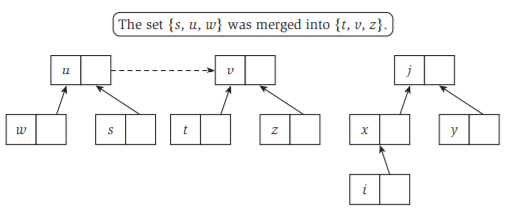
\includegraphics[scale=1.3]{Imagenes-Seccion4/fig4_12.PNG}
\textbf{El conjunto $\{s, u, w\}$ fue mezclado en $\{t, v, z\}$}
\caption{\textbf{Figura 4.12:} Una estructura de datos de Union-Find utilizando punteros. La estructura de datos tiene solo dos conjuntos en este momento, nombrados después de los nodos $v$ y $j$. La flecha discontinua de $u$ a $v$ es el resultado de la última operación de la Unión. Para responder una consulta Buscar, seguimos las flechas hasta que llegamos a un nodo que no tiene una flecha saliente. Por ejemplo, responder a la consulta Buscar ($i$) implicaría seguir las flechas $i$ a $x$, y luego $x$ a $j$.}
\end{figure}



\colorbox{mygray}{\parbox{15cm}{
\textbf{(4.24)}Considere la implementación anterior basada en apuntador de la estructura de datos de búsqueda de unión para algún conjunto $S$ de tamaño $n$, donde las uniones mantienen el nombre del conjunto más grande. Una operación Unión toma $O(1)$ vez, MakeUnionFind ($S$) toma $O (n)$ tiempo, y una operación Find toma $O(log n)$ tiempo.}}\\

\textbf{Prueba}. Las declaraciones sobre Union y MakeUnionFind son fáciles de verificar. El tiempo para evaluar Find ($v$) para un nodo $v$ es la cantidad de veces que el conjunto que contiene el nodo v cambia su nombre durante el proceso. Según la convención de que la unión conserva el nombre del conjunto más grande, se deduce que cada vez que cambia el nombre del conjunto que contiene el nodo $v$, el tamaño de este conjunto se duplica al menos. Como el conjunto que contiene $v$ comienza en el tamaño 1 y nunca es mayor que $n$, su tamaño puede duplicarse a lo sumo $log_2n$ veces, por lo que puede haber como máximo $log_2n$ cambios de nombre\\

\textbf{Futuras mejoras}

A continuación, analizaremos brevemente una optimización natural en la estructura de datos UnionFind basada en punteros que tiene el efecto de acelerar las operaciones de búsqueda. Estrictamente hablando, esta mejora no será necesaria para nuestros propósitos en este libro: para todas las aplicaciones de las estructuras de datos Union-Find que consideramos, el tiempo $O(log n)$ por operación es lo suficientemente bueno en el sentido de que la mejora en el el tiempo para las operaciones no se traduciría en mejoras en el tiempo total de ejecución de los algoritmos donde los usamos. (Las operaciones de UnionFind no serán el único cuello de botella computacional en el tiempo de ejecución de estos algoritmos).\\

Para motivar la versión mejorada de la estructura de datos, primero analicemos un caso malo para el tiempo de ejecución de la estructura de datos Union-Find basada en punteros. Primero construimos una estructura donde una de las operaciones Find tarda aproximadamente tiempo $log(n)$. Para hacer esto, podemos tomar repetidamente Uniones de conjuntos de igual tamaño. Supongamos que v es un nodo para el cual la operación Find ($v$) tarda aproximadamente tiempo $log n$. Ahora podemos emitir Find ($v$) repetidamente y toma log n para cada llamada. Tener que seguir la misma secuencia de punteros de log n cada vez para encontrar el nombre del conjunto que contiene v es bastante redundante: después de la primera solicitud de Buscar ($v$), ya "conocemos" el nombre $x$ del conjunto que contiene $v$, y también sabemos que todos los otros nodos que hemos tocado durante nuestro camino desde $v$ hasta el nombre actual también están contenidos en el conjunto $x$. Por lo tanto, en la implementación mejorada, comprimiremos la ruta que seguimos después de cada operación Buscar al restablecer todos los punteros a lo largo de la ruta para señalar el nombre actual del conjunto. No se pierde información al hacer esto y hace que las siguientes operaciones de búsqueda se ejecuten más rápidamente. Vea la Figura 4.13 para una estructura de datos Union-Find y el resultado de Find ($v$) usando la compresión de ruta.\\


\begin{figure}[h]
\centering
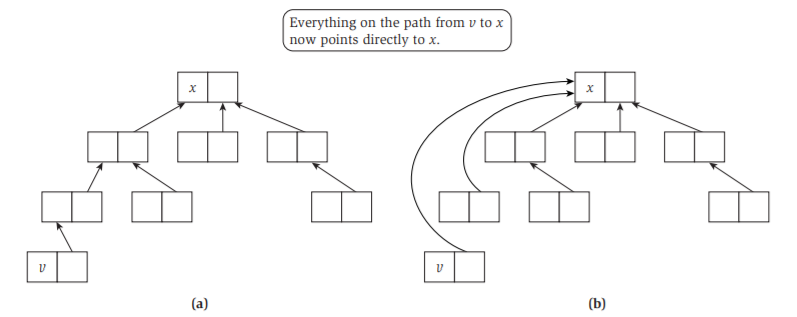
\includegraphics[scale=0.9]{Imagenes-Seccion4/fig4_13.PNG}
\end{figure}
\textbf{Figura 4.13}(a) Una instancia de una estructura de datos de búsqueda de la Unión; y (b) el resultado de la operación Find ($v$) en esta estructura, usando la compresión de ruta.\\


Ahora considere el tiempo de ejecución de las operaciones en la implementación resultante. Como antes, una operación de la Unión toma $O(1)$ tiempo y MakeUnionFind ($S$) toma $O(n)$ tiempo para configurar una estructura de datos para un conjunto de tamaño $n$. ¿Cómo cambió el tiempo requerido para una operación Find ($v$)? Algunas operaciones Buscar todavía pueden tomar hasta tiempo log $n$; y para algunas operaciones Buscar realmente aumentamos\\

En resumen, tenemos\\


\colorbox{mygray}{\parbox{15cm}{
\textbf{(4.25)}El algoritmo de Kruskal se puede implementar en un grafo con $n$ nodos y $m$ aristas para ejecutar en el tiempo $O(mlogn)$.}}\\

\subsection{Ejecricios resueltos}

\subsubsection{Ejercicio 1}

Supongamos que tres de sus amigos, inspirados por la película de terror The Blair Witch Project, han decidido caminar por el sendero de los Apalaches este verano. Quieren caminar tanto como sea posible por día pero, por razones obvias, no antes de que oscurezca. En un mapa, han identificado un gran conjunto de buenos puntos de parada para acampar, y están considerando el siguiente sistema para decidir cuándo detenerse por el día. Cada vez que llegan a un punto de detención potencial, determinan si pueden llegar al siguiente antes del anochecer. Si pueden hacerlo, entonces siguen caminando; de lo contrario, se detienen.\\


A pesar de muchos inconvenientes importantes, afirman que este sistema tiene una buena característica. "Dado que solo caminamos a la luz del día", afirman, "minimiza el número de paradas de campamento que tenemos que hacer".\\

¿Es esto cierto? El sistema propuesto es un algoritmo ávido, y deseamos determinar si se minimiza el número de paradas necesarias.\\

Para hacer esta pregunta precisa, hagamos el siguiente conjunto de suposiciones simplificadoras. Modelaremos el sendero de los Apalaches como un segmento de línea larga de longitud $L$, y supongamos que sus amigos pueden caminar $d$ millas por día (independientemente del terreno, las condiciones climáticas, etc.). Supondremos que los posibles puntos de detención se encuentran a distancias $x_1, x_2, ..., x_n$ desde el inicio del recorrido. También asumiremos (muy generosamente) que sus amigos siempre tienen la razón cuando estiman si pueden llegar al siguiente punto de detención antes del anochecer.\\

Diremos que un conjunto de puntos de detención es válido si la distancia entre cada par adyacente es como máximo $d$, la primera es a una distancia como máximo $d$ desde el inicio del recorrido, y la última está a una distancia máxima de $d$ fin del camino. Por lo tanto, un conjunto de puntos de detención es válido si se puede acampar solo en estos lugares y aún así cruzar todo el camino. Supondremos, naturalmente, que el conjunto completo de $n$ puntos de detención es válido; de lo contrario, no habría forma de hacerlo todo el camino.\\

Ahora podemos formular la pregunta de la siguiente manera. ¿Es el algoritmo ávido de sus amigos, - caminando el mayor tiempo posible cada día -, óptimo, en el sentido de que encuentra un conjunto válido cuyo tamaño es lo más pequeño posible?\\


\textbf{Solución}. A menudo, un algoritmo ávido parece correcto cuando lo encuentra por primera vez, por lo que antes de sucumbir demasiado a su atractivo intuitivo, es útil preguntar: ¿por qué no funciona? ¿De qué deberíamos estar preocupados?\\

Hay una preocupación natural con este algoritmo: ¿no ayudaría detenerse temprano algún día, para estar mejor sincronizado con las oportunidades de acampar en días futuros? Pero si lo piensas bien, comienzas a preguntarte si esto realmente podría suceder. ¿Podría haber realmente una solución alternativa que quede rezagada intencionalmente detrás de la solución codiciosa, y luego aumente de velocidad y pase la codiciosa solución? ¿Cómo podría pasar, dado que la solución codiciosa viaja lo más posible cada día?\\

Esta última consideración comienza a verse como el esquema de un argumento basado en el principio de "mantenerse adelante" de la Sección 4.1. Tal vez podamos demostrar que, siempre que la estrategia ambiciosa de acampar venza en un día determinado, ninguna otra solución puede alcanzarla y adelantarla al día siguiente.\\

Ahora convertimos esto en una prueba que muestra que el algoritmo es realmente óptimo, identificando un sentido natural en el que los puntos de detención eligen "mantenerse por delante" de cualquier otro conjunto legal de puntos de detención. Aunque estamos siguiendo el estilo de prueba de la Sección 4.1, vale la pena notar un interesante contraste con el Problema de Programación de Intervalos: allí necesitábamos probar que un algoritmo ávido maximizaba una cantidad de interés, mientras que aquí buscamos minimizar una cierta cantidad.\\

Sea $R = {x_{p1},..., x_{pk}}$ el conjunto de puntos de detención elegidos por el algoritmo ávido, y suponga, por contradicción, que existe un conjunto de puntos de detención válido más chicos; llamemos a este conjunto más pequeño $S = {x_{q1}, ..., x_{qm}}$, con $m<k$.\\

Para obtener una contradicción, primero mostramos que el punto de detención alcanzado por el algoritmo ávido en cada día j está más allá del punto de detención alcanzado en la solución alternativa. Es decir:\\

\textbf{(4.40)} Para cada $j=1,2,...,m$, tenemos $x_{pj} ≥ x_{qj}$.\\

\textbf{Prueba}. Probamos esto por inducción en $j$. El caso $j = 1$ se sigue directamente de la definición del algoritmo ávido: tus amigos viajan el mayor tiempo posible el primer día antes de detenerse. Ahora, supongamos que $j> 1$ y supongamos que la afirmación es verdadera para todo $i<j$. Entonces $x_{q_j} − x_{q_j-} ≤ d$ ya que S es un conjunto válido de puntos de parada, y $x_{q_j} − x_{p_j−1} ≤ x_{q_j} − x_{q_j−1}$ desde $x_{p_j-1} ≥ x_{q_j-1}$ por la hipótesis de inducción. Combinando estas dos desigualdades, tenemos\\

Esto significa que tus amigos tienen la opción de caminar desde $x_{p_j-1}$ a $x_{q_j}$ en un día; y por lo tanto, la ubicación $x_{p_j}$ en la que finalmente se detienen solo puede estar más adelante que $x_{q_j}$. (Tenga en cuenta la similitud con la prueba correspondiente para el problema de programación de intervalos: aquí también el algoritmo ávido se mantiene al frente porque, en cada paso, la elección hecha por la solución alternativa es una de sus opciones válidas).\\

El enunciado (4.40) implica en particular que $x_{q_m} ≤ x_{p_m}$. Ahora, si $m<k$, entonces debemos tener $x_{p_m}<L-d$, porque de lo contrario sus amigos nunca habrían necesitado detenerse en la ubicación $x_{p_m} + 1$. Combinando estas dos desigualdades, hemos concluido que $x_{q_m}<L-d$; pero esto contradice la suposición de que S es un conjunto válido de puntos de detención.\\

En consecuencia, no podemos tener $m<k$, por lo que hemos demostrado que el algoritmo ávido produce un conjunto válido de puntos de detención del tamaño mínimo posible.\\


\subsubsection{Ejercicio 2}

Tus amigos están comenzando una compañía de seguridad que necesita obtener licencias para diferentes piezas de software criptográfico. Debido a las regulaciones, solo pueden obtener estas licencias a razón de, como máximo, una por mes. Cada licencia se está vendiendo actualmente por un precio de \$100. Sin embargo, todos son cada vez más caros de acuerdo con las curvas de crecimiento exponencial: en particular, el costo de licencia aumenta en un factor de $r_j>1$ cada mes, donde $r_j$ es un parámetro dado. Esto significa que, si la licencia j se compra en t meses, costará 100 · $r^t_j$. Supondremos que todas las tasas de crecimiento de precios son distintas; es decir, $r_i != r_j$ para licencias $i != j$ (aunque comienzan con el mismo precio de \$100).\\

La pregunta es: dado que la compañía solo puede comprar como máximo una licencia al mes, ¿en qué orden debe comprar las licencias para que la cantidad total de dinero que gasta sea lo más pequeña posible? Proporcione un algoritmo que tome las n tasas de crecimiento de precios $r_1,r_2,...,rn$, y calcule un orden en el que comprar las licencias para minimizar la cantidad total de dinero gastado. El tiempo de ejecución de su algoritmo debe ser polinomial en n.\\

\textbf{Solución:} Dos conjeturas naturales para una buena secuencia serían ordenar el $r_i$ en orden decreciente, o ordenarlos en orden creciente. Frente a alternativas como esta, es perfectamente razonable resolver un pequeño ejemplo y ver si el ejemplo elimina al menos uno de ellos. Aquí podríamos probar $r_1=2$, $r_2=3$ y $r_3=4$. Comprar las licencias en orden creciente resulta en un costo total de $100(2+3^2+4^3) =7,500$, al comprarlos en orden decreciente resulta en un costo total de $100(4+3^2+2^3)=2,100$.\\

Esto nos dice que aumentar el orden no es el camino a seguir. (Por otro lado, no nos dice inmediatamente que el orden decreciente es la respuesta correcta, pero nuestro objetivo era simplemente eliminar una de las dos opciones).\\

 Probemos demostrando que ordenar el $r_i$ en orden decreciente siempre da la solución óptima. Cuando un algoritmo ávido funciona para problemás como este, en los cuales ponemos un conjunto de cosas en un orden óptimo, hemos visto en el texto que a menudo es efectivo intentar probar la corrección usando un argumento de intercambio.\\
 
Para hacer esto aquí, supongamos que hay una solución óptima O que difiere de nuestra solución S. (En otras palabras, S consiste en las licencias ordenadas en orden decreciente). Entonces, esta solución óptima O debe contener una inversión, es decir, debe haber dos meses vecinos t y t + 1 de manera que la tasa de aumento de precio de la licencia comprada en el mes t (denotemos por $r_t$) sea menor que la comprada en el mes t + 1 (de manera similar, usamos $r_t+1$ para denotar esto). Es decir, tenemos $r_t < r_t + 1$.\\

Reivindicamos que cambiando nuestras compras, podemos mejorar la solución óptima, lo que contradice la suposición de que O era óptimo. Por lo tanto, si tenemos éxito en mostrar esto, demostraremos con éxito que nuestro algoritmo es realmente el correcto.
Tenga en cuenta que si cambiamos estas dos compras, el resto de las compras tienen un precio idéntico. En O, el monto pagado durante los dos meses involucrados en el canje es $100(r^t_t + r^{t+1}_{t+1})$ Por otro lado, si intercambiáramos estas dos compras, pagaríamos  $100(r^t_{t+1} + r^{t+1}_{t})$ Como la constante 100 es común para ambas expresiones, queremos mostrar que el segundo término es menor que el primero. Entonces queremos mostrar que\\

$r^t_{t+1} + r^{t+1}_{t} < r^t_t + r^{t+1}_{t+1}$\\
$r^{t+1}_{t} - r^t_{t} < r^{t+1}_{t+1} - r^t_{t+1}$\\
$r^{t}_{t}(r_t - 1) < r^{t}_{t+1} (r_{t+1}-1)$\\

Pero esta última desigualdad es verdadera simplemente porque $r_i> 1$ para todo $i$ y desde $r_t<r_t+1$. Esto concluye la prueba de corrección. El tiempo de ejecución del algoritmo de referencia es $O(nlogn)$, ya que la clasificación lleva mucho tiempo y el resto (salida) es lineal. Entonces, el tiempo total de ejecución es $O(nlog n)$.\\

\textbf{Nota}: Es interesante observar que las cosas se vuelven mucho menos sencillas si variamos esta pregunta incluso un poco. Supongamos que, en lugar de comprar licencias cuyos precios aumentan, intente vender equipos cuyo costo se está depreciando. El ítem i se deprecia a un factor de $r_i<1$ por mes, a partir de \$100, así que si lo vendes en t meses, recibirás $100.r^t_i$. (En otras palabras, las tasas exponenciales ahora son menores que 1, en lugar de ser mayores a 1). Si solo puede vender un artículo por mes, ¿cuál es el orden óptimo para venderlos? Aquí, resulta que hay casos en que la solución óptima no pone las tasas en orden creciente o decreciente (como en la entrada 3/4, 1/2, 1/100).\\

\subsubsection{Ejercicio 3}

Supongamos que se le asigna un grafo $G$ conexo, con costos de arista que puede suponer que son todos distintos. $G$ tiene $n$ vértices y $m$ aristas. Se especifica una arista $e$ particular de $G$. Proporcione un algoritmo con tiempo de ejecución $O(m+n)$ para decidir si $e$ está contenido en un árbol de expansión mínimo de $G$.\\

\textbf{Solución}. Del texto, sabemos dos reglas por las cuales podemos concluir si una arista $e$ pertenece a un árbol de expansión mínimo: la Propiedad de corte (4.17) dice que $e$ está en cada árbol de expansión mínimo cuando es el cruce de arista más barata de algún conjunto $S$ al complemento $V - S$; y la Propiedad del ciclo (4.20) dice que $e$ no está en ningún árbol de expansión mínimo si es la arista más cara en algún ciclo $C$. Veamos si podemos hacer uso de estas dos reglas como parte de un algoritmo que resuelve este problema en tiempo lineal.\\

Las Propiedades de Corte y Ciclo están esencialmente hablando de cómo $e$ se relaciona con el conjunto de aristas que son más baratas que $e$. La Propiedad de Corte puede verse como preguntando: ¿Hay algún conjunto de $S⊆V$ para que para pasar de $S$ a $V-S$ sin usar $e$, tengamos que usar una arista que sea más cara que $e$? Y si pensamos en el ciclo $C$ en la declaración de la Propiedad del ciclo, recorrer el "camino largo" alrededor de $C$ (evitando $e$) se puede ver como una ruta alternativa entre los extremos de e que solo usa aristas más baratas.\\

Al juntar estas dos observaciones, sugerimos que intentemos probar la siguiente declaración.\\

\textbf{(4.41)} La arista $e=(v,w)$ no pertenece a un árbol de expansión mínimo de $G$ si y solo si $v$ y $w$ se pueden unir mediante un camino que consista completamente de aristas que son más baratas que $e$\\

\textbf{Prueba}. Primero suponga que $P$ es una camino $v-w$ que consiste completamente de aristas más baratas que $e$. Si agregamos $e$ a $P$, obtenemos un ciclo en el que $e$ es la arista más cara. Por lo tanto, por la Propiedad del ciclo, $e$ no pertenece a un árbol de expansión mínimo de $G$.\\

Por otro lado, supongamos que $v$ y $w$ no pueden unirse mediante un camino que consista en su totalidad en aristas más baratas que $e$. Ahora identificaremos un conjunto $S$ para el cual $e$ es la arista más barata con un extremo en $S$ y el otro en $V-S$; si podemos hacer esto, la Propiedad de Corte implicará que $e$ pertenece a cada árbol de expansión mínimo. Nuestro conjunto $S$ será el conjunto de todos los nodos a los que se puede llegar desde $v$ utilizando un camino que consta únicamente de aristas que son más baratas que $e$. Según nuestra suposición, tenemos $w \in V-S$. Además, por la definición de $S$, no puede haber una arista $f=(x,y)$ que sea más barata que $e$, y para el cual un extremo $x$ se encuentra en $S$ y el otro en $d$ y yace en $V-S$. De hecho, si existiera dicho $f$, entonces como el nodo $x$ es alcanzable desde $v$ usando solo aristas más baratas que $e$, el nodo y también sería accesible. Por lo tanto, $e$ es la arista más barata con un extremo en $S$ y el otro en $V-S$, como se desee, y así terminamos.$\blacksquare$\\

Dado este hecho, nuestro algoritmo ahora es simplemente el siguiente. Formamos un grafo $G$ al eliminar de $G$ todas las aristas de peso mayor que $C_e$ (así como también eliminamos $e$). Luego usamos uno de los algoritmos de conectividad del Capítulo 3 para determinar si hay un camino de $v$ a $w$ en $G$. La declaración (4.41) dice que $e$ pertenece a un árbol de expansión mínimo si y solo si no existe dicho camino.\\

El tiempo de ejecución de este algoritmo es $O(m+n)$ para construir $G$, y $O(m+n)$ para probar un camino de $v$ a $w$\\


\section{Divide y vencerás}

Dividir y conquistar se refiere a una clase de técnicas algorítmicas en la que uno divide la entrada en varias partes, resuelve el problema en cada parte recursivamente y luego combina las soluciones a estos subproblemas en una solución global. En muchos casos, puede ser un método simple y poderoso.\\

Analizar el tiempo de ejecución de un algoritmo de divide y vencer generalmente implica resolver una relación de recurrencia que limita el tiempo de ejecución recursivamente en términos del tiempo de ejecución en instancias más pequeñas. Comenzamos el capítulo con una discusión general de las relaciones de recurrencia, ilustrando cómo surgen en el análisis y describiendo los métodos para elaborar los límites superiores a partir de ellos.\\

A continuación, ilustramos el uso de dividir y conquistar con aplicaciones a varios dominios diferentes: calcular una función de distancia en diferentes clasificaciones de un conjunto de objetos; encontrar el par de puntos más cercano en el avión; multiplicando dos enteros; y suavizar una señal ruidosa. Dividir y conquistar también aparecerá en capítulos posteriores, ya que es un método que a menudo funciona bien cuando se combina con otras técnicas de diseño de algoritmos. Por ejemplo, en el Capítulo 6 lo veremos combinado con la programación dinámica para producir una solución eficiente desde el punto de vista del espacio para un problema de comparación de secuencia fundamental, y en el Capítulo 13 lo veremos combinado con la aleatorización para obtener un algoritmo simple y eficiente para calcular la mediana de un conjunto de números.\\

Una cosa a tener en cuenta sobre muchos escenarios en los que se aplica dividir y conquistar, incluidos estos, es que el algoritmo de fuerza bruta natural ya puede ser un tiempo polinomial, y la estrategia de dividir y vencer sirve para reducir el tiempo de ejecución a un polinomio inferior. Esto está en contraste con la mayoría de los problemas en los capítulos anteriores, por ejemplo, donde la fuerza bruta era exponencial y el objetivo en el diseño de un algoritmo más sofisticado era lograr cualquier tipo de tiempo de ejecución de polinomios. Por ejemplo, discutimos en el Capítulo 2 que el algoritmo natural de fuerza bruta para encontrar el par más cercano entre n puntos en el plano simplemente mediría todas las ($n^{2}$) distancias, para un tiempo de ejecución (polinomial) de ($n^{2}$). Usando divide y vencerás, mejoraremos el tiempo de ejecución hasta $O(n log n)$. En un nivel alto, entonces, el tema general de este capítulo es el mismo que hemos visto anteriormente: que la mejora en la búsqueda de fuerza bruta es un obstáculo conceptual fundamental para resolver un problema de manera eficiente, y el diseño de algoritmos sofisticados puede lograr esto. La diferencia es simplemente que la distinción entre búsqueda de fuerza bruta y una solución mejorada aquí no siempre será la distinción entre exponencial y polinomio.\\

\subsection{Una primera recurrencia: el algoritmo Mergesort}

Para motivar el enfoque general del análisis de los algoritmos de división y conquista, comenzamos con el algoritmo Mergesort. Discutimos brevemente el algoritmo Mergesort en el Capítulo 2, cuando analizamos los tiempos de ejecución comunes para los algoritmos. Mergesort ordena una lista dada de números dividiéndolos primero en dos mitades iguales, clasificando cada mitad por separado por recursión, y luego combinando los resultados de estas llamadas recursivas, en la forma de las dos mitades ordenadas, utilizando el algoritmo de tiempo lineal para la fusión listas ordenadas que vimos en el Capítulo 2.\\

Para analizar el tiempo de ejecución de Mergesort, resumiremos su comportamiento en la siguiente plantilla, que describe muchos algoritmos comunes de dividir y conquistar\\

(†) Divida la entrada en dos partes de igual tamaño; resuelve los dos subproblemas en estas piezas por separado por recursión; y luego combine los dos resultados en una solución global, gastando solo tiempo lineal para la división inicial y la recombinación final.\\


En Mergesort, como en cualquier algoritmo que se adapte a este estilo, también necesitamos un caso base para la recursión, por lo general tenerlo "de fondo" en las entradas de algún tamaño constante. En el caso de Mergesort, supondremos que una vez que la entrada se ha reducido al tamaño 2, detenemos la recursión y clasificamos los dos elementos simplemente comparándolos entre sí.\\

Considere cualquier algoritmo que se ajuste al patrón en (†), y deje que $T(n)$ denote su peor tiempo de ejecución en instancias de entrada de tamaño $n$. Suponiendo que $n$ es par, el algoritmo pasa el tiempo $O (n)$ para dividir la entrada en dos piezas de tamaño $n/2$ cada una; luego pasa el tiempo $T(n/2)$ para resolver cada uno (ya que $T(n/2)$ es el peor tiempo de ejecución para una entrada de tamaño $n/2$); y finalmente gasta $O(n)$ tiempo para combinar las soluciones de las dos llamadas recursivas. Por lo tanto, el tiempo de ejecución $T(n)$ satisface la siguiente relación de recurrencia\\

\textbf{(5.1)} Por alguna $c$ constante $T(n) ≤ 2T(n/2) + cn$ con $n>2$, $T(2) ≤ c$\\

La estructura de (5.1) es típica de lo que parecerán las recurrencias: hay una desigualdad o ecuación que limita a $T(n)$ en términos de una expresión que involucra $T(k)$ para valores más pequeños $k$; y hay un caso base que generalmente dice que $T(n)$ es igual a una constante cuando $n$ es una constante. Tenga en cuenta que también se puede escribir (5.1) más informalmente como $T(n)≤ 2T(n / 2) + O (n)$, suprimiendo la constante $c$. Sin embargo, generalmente es útil hacer $c$ explícita al analizar la recurrencia.\\

Para mantener la exposición más simple, generalmente asumiremos que los parámetros como $n$ son incluso cuando sea necesario. Este es un uso algo impreciso; sin esta suposición, las dos llamadas recursivas estarían en problemas de tamaño? $\left \lfloor n/2 \right \rfloor$ y $\left \lceil n/2 \right \rceil$, y la relación de recurrencia diría que

$T(n) ≤ T(\left \lfloor n/2 \right \rfloor) + T(\left \lceil n/2 \right \rceil) + cn$

PAra $n ≥ 2$ sin embargo, para todas las recurrencias que consideramos aquí (y para la mayoría que surgen en la práctica), los límites asintóticos no se ven afectados por la decisión de ignorar todos los pisos y techos, y hace que la manipulación simbólica sea mucho más limpia.\\

Ahora (5.1) no proporciona explícitamente un límite asintótico en la tasa de crecimiento de la función $T$; más bien, especifica $T(n)$ implícitamente en términos de sus valores en entradas más pequeñas. Para obtener un límite explícito, necesitamos resolver la relación de recurrencia de modo que $T$ aparezca solo en el lado izquierdo de la desigualdad, no en el lado derecho también.\\

La resolución de recurrencia es una tarea que se ha incorporado a varios sistemas de álgebra computarizada estándar, y la solución para muchas recurrencias estándar ahora se puede encontrar por medios automáticos. Sin embargo, todavía es útil comprender el proceso de resolver recurrencias y reconocer qué recurrencias conducen a buenos tiempos de ejecución, ya que el diseño de un algoritmo de divide y vencerás eficiente está estrechamente entrelazado con una comprensión de cómo una relación de recurrencia determina un tiempo de ejecución\\

\textbf{Enfoques para resolver las recurrencias}
Hay dos formas básicas para resolver una recurrencia, cada una de las cuales describiremos con más detalle a continuación.\\

\begin{enumerate}
\item La forma más natural e intuitiva de buscar una solución para una recurrencia es "desenrollar" la recursión, teniendo en cuenta el tiempo de ejecución en los primeros niveles e identificar un patrón que pueda continuar a medida que se expande la recursión. Luego se suman los tiempos de ejecución en todos los niveles de la recursión (es decir, hasta que "toca fondo" en los subproblemas de tamaño constante) y, por lo tanto, llega a un tiempo de ejecución total.

\item  Una segunda forma es comenzar con una estimación de la solución, sustituirla por la relación de recurrencia y verificar que funcione. Formalmente, uno justifica este plug-in usando un argumento por inducción en n. Existe una variante útil de este método en la que uno tiene una forma general para la solución, pero no tiene valores exactos para todos los parámetros. Al dejar estos parámetros no especificados en la sustitución, a menudo se pueden resolver según sea necesario
\end{enumerate}
    
Ahora discutimos cada uno de estos enfoques, usando la recurrencia en (5.1) como ejemplo\\
    
\textbf{Desenrollando la recurrencia de Mergesort} \\

Comencemos con el primer enfoque para resolver la recurrencia en (5.1). El argumento básico se muestra en la Figura 5.1.\\

\begin{itemize}

\item Análisis de los primeros niveles: en el primer nivel de recursión, tenemos un único problema de tamaño n, que lleva más tiempo $c_n$ más el tiempo empleado en todas las llamadas recursivas posteriores. En el siguiente nivel, tenemos dos problemas, cada uno de tamaño $n/2$. Cada uno de estos lleva un tiempo máximo de $c_n /2$, para un total de $c_n$ como máximo, de nuevo más el tiempo en llamadas recursivas posteriores. En el tercer nivel, tenemos cuatro problemas, cada uno de tamaño $n/4$, cada uno tomando como máximo $c_n/4$, para un total de como máximo $c_n$.    

\end{itemize}

\begin{figure}[h]
\centering
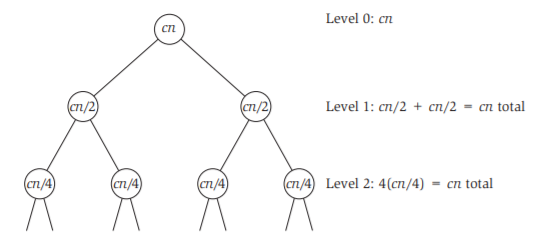
\includegraphics[width=0.7\textwidth]{Imagenes-Seccion5/fig5_1.PNG}
\caption{Desenrollando la recurrencia $T (n) ≤ 2T (n / 2) + O (n)$}
\end{figure}

\begin{itemize}

\item Identificando un patrón: ¿Qué está pasando en general? En el nivel $j$ de la recursión, el número de subproblemas se ha duplicado $j$ veces, por lo que ahora hay un total de $2j$. Cada uno de ellos se ha encogido correspondientemente en un factor de dos veces $j$, por lo que cada uno tiene un tamaño $n/2j$ y, por lo tanto, cada uno lleva como máximo $c_n/2j$. Por lo tanto, el nivel $j$ contribuye con un total de como máximo $2j$ ($c_n / 2j$) = $c_n$ al tiempo total de ejecución.

\item Sumando todos los niveles de recursión: hemos encontrado que la recurrencia en (5.1) tiene la propiedad de que el mismo límite superior de $c_n$ se aplica a la cantidad total de trabajo realizado en cada nivel. El número de veces que la entrada se debe reducir a la mitad para reducir su tamaño de $n$ a 2 es $log2 n$. Así que sumando el trabajo $c_n$ sobre los niveles $log n$ de recursión, obtenemos un tiempo de ejecución total de $O(nlogn)$.

\end{itemize}
    
Resumimos esto en el siguiente teorema.
    
 \colorbox{mygray}{\parbox{15cm}{
\textbf{(5.2)} Cualquier función $T$ (·) que satisfaga a (5.1) está limitada por $O(nlogn)$, cuando $n>1$.}}\\    


Sustituyendo una Solución en la Repetición de Mergesort

El argumento que establece (5.2) puede usarse para determinar que la función T (n) está limitada por O (n log n). Si, por otro lado, tenemos una estimación del tiempo de ejecución que queremos verificar, podemos hacerlo conectándolo a la repetición de la siguiente manera.\\

Supongamos que creemos que $T(n) ≤ cn log_2n$ para todo $n≥2$, y queremos verificar si esto es realmente cierto. Esto se cumple claramente para $n=2$, ya que en este caso $cn log_2n = 2c$, y (5.1) explícitamente nos dice que $T(2) ≤ c$. Ahora supongamos, por inducción, que $T(m) ≤ cm log_2 m$ para todos los valores de $m$ menores que $n$, y queremos establecer esto para $T(n)$. Hacemos esto escribiendo la recurrencia para $T(n)$ y conectando la desigualdad $T(n/2) ≤ c(n/2) log_2 (n/2)$. Luego simplificamos la expresión resultante al notar que $log_2(n/2) = (log_2n) - 1$. Aquí está el cálculo completo\\

$T(n) ≤ 2T(n/2) + cn$\\
$≤ 2c(n/2) log_2(n/2) + cn$\\
$= cn[(log_2 n) − 1]+ cn$\\
$= (cn log_2 n) − cn + cn$\\
$= cn log_2 n.$\\

Esto establece el límite que queremos para $T(n)$, suponiendo que se mantiene para valores menores $m<n$, y así completa el argumento de inducción.\\


\textbf{Un enfoque que usa la sustitución parcial}

Hay un tipo de sustitución algo más débil que uno puede hacer, en el cual uno adivina la forma general de la solución sin fijar los valores exactos de todas las constantes y otros parámetros desde el principio.\\

Específicamente, supongamos que creemos que $T(n) = O(n log n)$, pero no estamos seguros de la constante dentro de la notación $O (·)$. Podemos usar el método de sustitución incluso sin estar seguros de esta constante, de la siguiente manera. Primero escribimos $T(n)≤knlog_b n$ para alguna constante $k$ y base $b$ que determinaremos más adelante. (En realidad, la base y la constante que necesitaremos están relacionadas entre sí, como vimos en el Capítulo 2 que uno puede cambiar la base del logaritmo simplemente cambiando la constante multiplicativa al frente).\\

Ahora nos gustaría saber si hay alguna opción de $k$ y $b$ que funcione en un argumento inductivo. Entonces probamos un nivel de inducción de la siguiente manera.\\

$T(n) ≤ 2T(n/2) + cn ≤ 2k(n/2) log_b(n/2) + cn$\\

Ahora es muy tentador elegir la base $b=2$ para el logaritmo, ya que vemos que esto nos permitirá aplicar la simplificación $log_2(n/2) = (log_2 n) − 1$. Continuando con esta elección, tenemos\\

$T(n) ≤ 2k(n/2) log_2(n/2) + cn$\\
$= 2k(n/2)[(log_2 n) − 1]+ cn$\\
$= kn[(log_2 n) − 1]+ cn$\\
$= (kn log_2 n) − kn + cn$\\

Finalmente, nos preguntamos: ¿Existe una opción de $k$ que haga que esta última expresión esté delimitada por $kn log_2 n$? La respuesta es claramente sí; solo tenemos que elegir cualquier $k$ que sea al menos tan grande como $c$, y obtenemos\\

$T(n) ≤ (kn log_2 n) − kn + cn ≤ kn log_2 n$\\

que completa la inducción.\\

Por lo tanto, el método de sustitución puede ser realmente útil para calcular las constantes exactas cuando se tiene una idea aproximada de la forma general de la solución.\\



\subsection{Otras relaciones de recurrencia}

Hemos elaborado la solución a una relación de recurrencia, (5.1), que aparecerá en el diseño de varios algoritmos de divide y conquistaras más adelante en este capítulo. Como una forma más de explorar este tema, ahora consideramos una clase de relaciones de recurrencia que generaliza (5.1) y mostramos cómo resolver las recurrencias de esta clase. Otros miembros de esta clase surgirán en el diseño de algoritmos tanto en este capítulo como en capítulos posteriores.\\

Esta clase más general de algoritmos se obtiene al considerar algoritmos de divide y vencerás que crean llamadas recursivas en $q$ subproblemas de tamaño $n / 2$ cada uno y luego combinan los resultados en tiempo $O (n)$. Esto corresponde a la recurrencia de Mergesort (5.1) cuando se utilizan $q = 2$ llamadas recursivas, pero a otros algoritmos les resulta útil generar $q> 2$ llamadas recursivas, o solo una llamada recursiva ($q = 1$). De hecho, veremos el caso $q> 2$ más adelante en este capítulo cuando diseñemos algoritmos para la multiplicación de enteros; y veremos una variante en el caso $q = 1$ mucho más adelante en el libro, cuando diseñemos un algoritmo aleatorizado para encontrar la mediana en el Capítulo 13.\\

Si $T (n)$ denota el tiempo de ejecución de un algoritmo diseñado en este estilo, entonces $T (n)$ obedece a la siguiente relación de recurrencia, que directamente generaliza (5.1) reemplazando $2$ con $q$:\\

\textbf{(5.3)} Por alguna constante $c$,\\
										$T(n) ≤ qT(n/2) + cn$\\
$cuando n> 2, y$\\
										$T(2) ≤ c.$\\

Ahora describimos cómo resolver (5.3) con los métodos que hemos visto anteriormente: desenrollar, sustituir y sustituir parcialmente. Tratamos los casos $q> 2$ y $q = 1$ por separado, ya que son cualitativamente diferentes entre sí, y diferentes del caso $q = 2$ también.\\

\textbf{El caso de $q> 2$ subproblemas}
Comenzamos desenrollando (5.3) en el caso $q> 2$, siguiendo el estilo que utilizamos anteriormente para (5.1). Veremos que la línea final termina siendo bastante diferente.\\
\begin{itemize}
\item Analizando los primeros niveles: Mostramos un ejemplo de esto para el caso $q = 3$ en la Figura 5.2. En el primer nivel de recursión, tenemos un único problema de tamaño $n$, que lleva más tiempo $c_n$ más el tiempo empleado en todas las llamadas recursivas posteriores. En el siguiente nivel, tenemos $q$ problemas, cada uno de tamaño $n / 2$. Cada uno de estos toma tiempo a lo sumo $c_n / 2$, para un total de a lo sumo $(q / 2) c_n$, nuevamente más el tiempo en llamadas recursivas subsiguientes. El siguiente nivel produce $q^2$ problemas de tamaño $n / 4$ cada uno, durante un tiempo total de $(q^2 / 4) c_n$. Desde $q> 2$, vemos que el trabajo total por nivel aumenta a medida que avanzamos en la recursión.\\

\item Identificando un patrón: En un nivel arbitrario $j$, tenemos $q^j$ instancias distintas, cada una de tamaño $n / 2^j$. Por lo tanto, el trabajo total realizado en el nivel $j$ es $q^j (cn / 2^j) = (q / 2)^j cn$.\\
\end{itemize}

\begin{figure}[h]
\centering
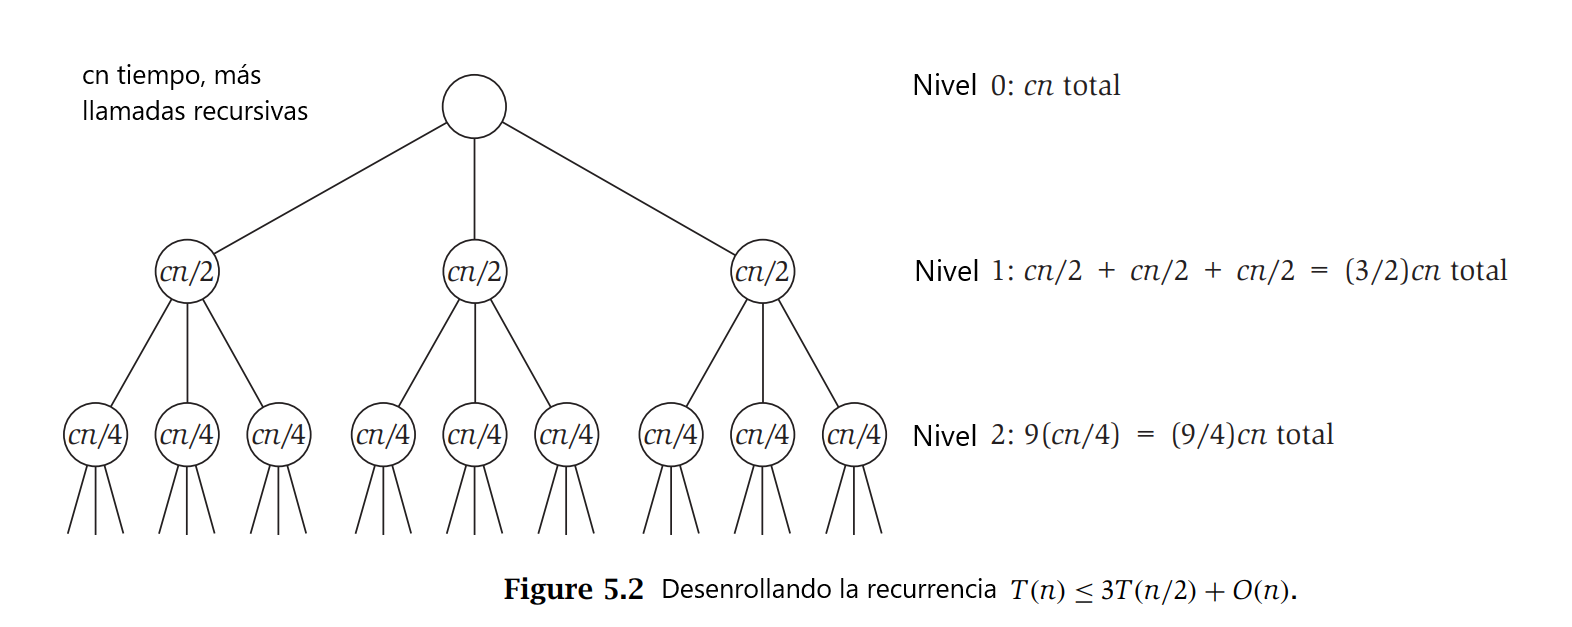
\includegraphics[scale=0.4]{Imagenes-Seccion5/Fig5_2.PNG}
\end{figure}
\begin{itemize}
\item Sumando todos los niveles de recursión: como antes, hay $log_2 n$ niveles de recursión, y la cantidad total de trabajo realizado es la suma de todos estos:
\end{itemize}

$T(n)\leq \sum_{j=0}^{log_2n-1}{(q/2)^j}cn=cn\sum_{j=0}^{log_2n-1}{(q/2)^j}$.

Esta es una suma geométrica, que consiste en potencias de $r = q / 2$. Podemos usar la fórmula para una suma geométrica cuando $r> 1$, que nos da la fórmula $T(n)\leq cn \left ( \frac{r^{log_2n}-1}{r-1} \right )\leq cn\left ( \frac{r^{log_2n}}{r-1} \right )$. Como apuntamos a un límite superior asintótico, es útil ver qué es simplemente una constante; podemos sacar el factor de $r - 1$ del denominador, y escribir la última expresión como $T(n)\leq \left ( \frac{c}{r-1} \right )nr^{log_2n}$.

Finalmente, necesitamos descubrir qué es $r^{log_2 n}$. Aquí usamos una identidad muy útil, que dice que, para cualquier $a> 1$ y $b> 1$, tenemos $a^{log b}=b^{log  a}$. Así	$r^{log_2n}=n^{log_2r}=n^{log_2(q/2)}=n^{(log_2q)-1}$.
          	
Así tenemo      				$T(n)\leq \left ( \frac{c}{r-1} \right )n*n^{(log_2q)-1}\leq \left ( \frac{c}{r-1} \right )n^{log_2q}=O(n^{log_2q})$.

Lo resumimos de la siguiente manera.\\
            
\textbf{(5.4)}Cualquier función $T$ (·) satisfactoria (5.3) con $q> 2$ está limitada por $O (n^{log_2 q})$.\\

Así que encontramos que el tiempo de ejecución es más que lineal, ya que $log_2 q> 1$, pero aún polinomial en $n$. Al conectar valores específicos de $q$, el tiempo de ejecución es $O (n^{log_2 3}) = O (n^{1.59})$ cuando $q = 3$; y el tiempo de ejecución es $O (n^{log_2 4}) = O (n^2)$ cuando $q = 4$. Este aumento en el tiempo de ejecución como $q$ aumenta tiene sentido, por supuesto, ya que las llamadas recursivas generan más trabajo para valores más grandes de $q$.\\

\textbf{Aplicación de la sustitución parcial} La aparición de $log_2 q$ en el exponente surge naturalmente de nuestra solución a (5.3), pero no es necesariamente una expresión que uno hubiera adivinado desde el principio. Ahora consideramos cómo un enfoque basado en la sustitución parcial en la recurrencia produce una forma diferente de descubrir este exponente.\\

Supongamos que la solución a (5.3), cuando $q> 2$, tiene la forma $T (n) ≤ k n^d$ para algunas constantes $k> 0$ y $d> 1$. Esta es una suposición bastante general, ya que ni siquiera hemos intentado especificar el exponente $d$ del polinomio. Ahora intentemos iniciar el argumento inductivo y ver qué restricciones necesitamos en $k$ y $d$. Tenemos $T(n) ≤ q T(n/2) + c_n$, y aplicando la hipótesis inductiva a $T (n / 2)$, esto se expande a $T(n)\leq qk\left ( \frac{n}{2} \right )^d+c_n=\frac{q}{2^d}k n^d+c_n$. 

Esto es notablemente cercano a algo que funciona: si elegimos $d$ para que $q / 2^d = 1$, entonces tenemos $T (n) ≤ k n^d + c_n$, que es casi correcto, excepto por el término extra $c_n$. Así que vamos a tratar con estos dos problemas: primero, cómo elegir $d$ para obtener $q / 2^d = 1$; y segundo, cómo deshacerse del término $c_n$.\\
Elegir $d$ es fácil: queremos $2d = q$, y entonces $d = log_2 q$. Por lo tanto, vemos que el exponente $log_2 q$ aparece de forma muy natural una vez que decidimos descubrir qué valor de $d$ funciona cuando se lo sustituye en la recurrencia.\\

Pero todavía tenemos que deshacernos del término $cn$. Para hacer esto, cambiamos la forma de nuestra suposición para $T(n)$ para restarla explícitamente. Supongamos que probamos la forma $T (n) ≤ kn^d -ln$, donde ahora hemos decidido que $d = log_2 q$ pero no hemos arreglado las constantes $k$ o $l$. Aplicando la nueva fórmula a $T (n / 2)$, esto se expande a
$t(n)\leq qk\left ( \frac{n}{2} \right )-ql\left ( \frac{n}{2} \right )+cn$\\
$=\frac{q}{2^d}kn^d-\frac{ql}{2}n+cn$\\
$=kn^d-\frac{ql}{2}n+cn$\\
$=kn^d-(\frac{ql}{2}-c)n$\\

Esto ahora funciona completamente, si simplemente elegimos l de modo que $(\frac{ql}{2}-c)=l$: en otras palabras,$l=2c(q-2)$. Esto completa el paso inductivo para $n$. También necesitamos manejar el caso base $n = 2$, y esto lo hacemos usando el hecho de que el valor de $k$ aún no se ha elegido: elegimos $k$ lo suficientemente grande para que la fórmula sea un límite superior válido para el caso $n = 2$ .\\

\textbf{El caso de un subproblema}

Ahora consideramos el caso de $q = 1$ en (5.3), ya que esto ilustra un resultado de otro tipo. Si bien no veremos una aplicación directa de la recurrencia para $q = 1$ en este capítulo, aparece una variación en el Capítulo 13, como mencionamos anteriormente.\\
Comenzamos desenrollando la recurrencia para tratar de construir una solución.\\

\begin{itemize}

\item Analizando los primeros niveles: Mostramos los primeros niveles de la recursión en la Figura 5.3. En el primer nivel de recursión, tenemos un único problema de tamaño $n$, que lleva más tiempo $cn$ más el tiempo empleado en todas las llamadas recursivas posteriores. El siguiente nivel tiene un problema de tamaño $n / 2$, que contribuye $cn / 2$, y el nivel posterior tiene un problema de tamaño $n / 4$, que contribuye con $cn / 4$. Entonces, vemos que, a diferencia del caso anterior, el trabajo total por nivel cuando q = 1 en realidad está disminuyendo a medida que avanzamos en la recursión.
\item Identificar un patrón: en un nivel arbitrario $j$, todavía tenemos solo una instancia; tiene tamaño $n / 2j$ y contribuye $cn / 2j$ al tiempo de ejecución.
\item Sumando todos los niveles de recursión: hay $log_2 n$ niveles de recursión, y la cantidad total de trabajo realizado es la suma de todos estos: $T(n)\leq \sum _{j=0}^{log_2n-1}\frac{cn}{2^j}=cn\sum _{j=0}^{log_2n-1}\left ( \frac{1}{2^j} \right )$.\\Esta suma geométrica es muy fácil de resolver; incluso si lo continuamos hasta el infinito, convergería a 2. Por lo tanto, tenemos $T(n) ≤ 2cn = O(n)$.
\end{itemize}

\begin{figure}[h]
\centering
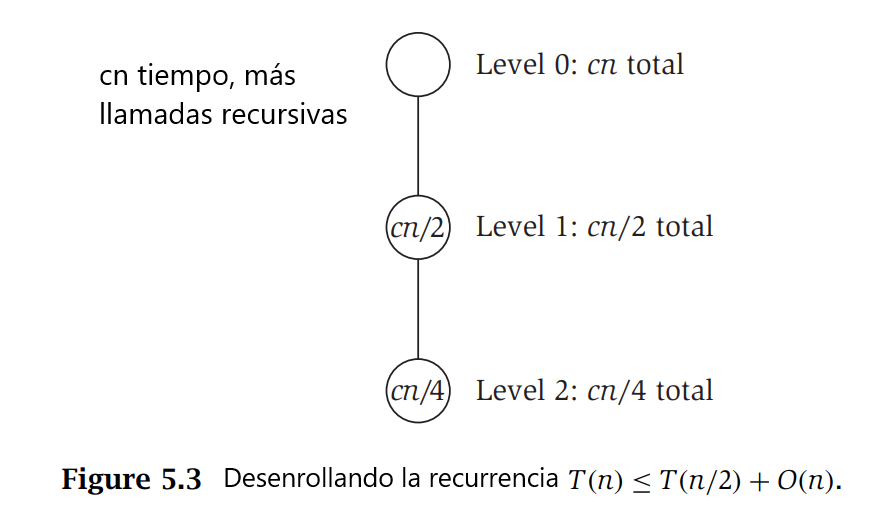
\includegraphics[scale=0.4]{Imagenes-Seccion5/Fig5_3.PNG}
\end{figure}
Lo resumimos de la siguiente manera.\\\\
\textbf{(5.5)} Cualquier función $T (·)$ que satisfaga (5.3) con $q = 1$ está limitada por $O (n)$.\\
Esto es contra intuitivo cuando lo ves por primera vez. El algoritmo está realizando $log n$ niveles de recursión, pero el tiempo de ejecución general sigue siendo lineal en $n$. El punto es que una serie geométrica con un exponente en descomposición es algo poderoso: la mitad del trabajo realizado por el algoritmo se realiza en el nivel superior de la recursión.\\

También es útil ver cómo la sustitución parcial en la recurrencia funciona muy bien en este caso. Supongamos como antes, que la forma de la solución es $T (n) ≤ kn^d$. Ahora tratamos de establecer esto por inducción usando (5.3), suponiendo que la solución se mantenga para el menor valor $n / 2$:\\\\
$T(n)\leq T(n/2)+cn\leq k\left ( \frac{n}{2} \right )^d+cn=\frac{k}{2^d}n^d+cn$.\\\\
Si ahora simplemente elegimos $d = 1$  y $k = 2c$, tenemos $T(n)\leq \frac{k}{2}n+cn=(\frac{k}{2}+c)n=kn$, que completa la inducción.\\

\textbf{El efecto del parámetro q}. Vale la pena reflexionar brevemente sobre el papel del parámetro $q$ en la clase de recurrencias $T (n) ≤ qT (n / 2) + O (n)$ definido por (5.3). Cuando $q = 1$, el tiempo de ejecución resultante es lineal; cuando $q = 2$, es $O (n log n)$; y cuando $q> 2$, es un polinomio vinculado con un exponente mayor que 1 que crece con $q$. La razón de este rango de tiempos de ejecución diferentes radica en que la mayor parte del trabajo se gasta en la recursión: cuando $q = 1$, el tiempo total de ejecución está dominado por el nivel superior, mientras que cuando $q> 2$ está dominado por el trabajo realizado subproblemas de tamaño constante en la parte inferior de la recursión. Visto de esta manera, podemos apreciar que la recurrencia para $q = 2$ representa realmente un "cuchillo": la cantidad de trabajo realizado en cada nivel es exactamente la misma, que es lo que produce el tiempo de ejecución $O (n log n)$.\\

\textbf{Una recurrencia relacionada:} $T (n) ≤ 2T (n / 2) + O (n2)$\\
Concluimos nuestra discusión con una relación de recurrencia final; es ilustrativa tanto como otra aplicación de una suma geométrica en descomposición y como un contraste interesante con la recurrencia (5.1) que caracteriza a Mergesort. Además, veremos una variante cercana en el Capítulo 6, cuando analicemos un algoritmo de divide y conquistaras para resolver el problema de alineación de secuencia usando una pequeña cantidad de memoria de trabajo.\\

La recurrencia se basa en la siguiente estructura de dividir y vencer. Divida la entrada en dos piezas de igual tamaño; resuelve los dos subproblemas en estas piezas por separado por recursión; y luego combine los dos resultados en una solución global, pasando tiempo cuadrático para la división inicial y la recombinación final.\\

Para nuestros propósitos aquí, notamos que este estilo de algoritmo tiene un tiempo de ejecución $T (n)$ que satisface la siguiente recurrencia.\\
\textbf{(5.6)}Por alguna constante $c$, $T(n) ≤ 2T(n/2) + cn^2$ cuando $n> 2$, y $T(2) ≤ c$.\\

La primera reacción de uno es adivinar que la solución será $T (n) = O (n^2 log n)$, ya que se ve casi idéntica a (5.1) excepto que la cantidad de trabajo por nivel es mayor por un factor igual al tamaño de entrada . De hecho, este límite superior es correcto (necesitaría un argumento más cuidadoso que el de la oración anterior), pero resultará que también podemos mostrar un límite superior más fuerte. Haremos esto desenrollando la recurrencia, siguiendo la plantilla estándar.\\

\begin{itemize}
\item  Análisis de los primeros niveles: en el primer nivel de recursión, tenemos un único problema de tamaño $n$, que lleva más tiempo $c_n^2$ más el tiempo empleado en todas las llamadas recursivas posteriores. En el siguiente nivel, tenemos dos problemas, cada uno de tamaño $n / 2$. Cada uno de estos toma tiempo a lo sumo $c (n / 2) ^2 = c_n^2 / 4$, para un total de $cn^2 / 2$ como máximo, de nuevo más el tiempo en las llamadas recursivas subsiguientes. En el tercer nivel, tenemos cuatro problemas, cada uno de tamaño $n / 4$, cada uno tomando como máximo $c (n / 4)^2 = cn^2 / 16$, para un total de como máximo $c_n^2 / 4$. Ya vemos que algo es diferente de nuestra solución a la recurrencia análoga (5.1); mientras que la cantidad total de trabajo por nivel permaneció igual en ese caso, aquí está disminuyendo.
\item Identificación de un patrón: En un nivel arbitrario $j$ de la recursión, hay $2^j$ subproblemas, cada uno de tamaño $n / 2^j$, y por lo tanto el trabajo total en este nivel está limitado por $2^j c (n/ 2^j)^2 = c_n^2 / 2^j$.
\item Sumando todos los niveles de recursión: habiendo llegado tan lejos en el cálculo, hemos llegado a casi exactamente la misma suma que tuvimos para el caso $q = 1$ en la recurrencia anterior. Tenemos $T(n)\leq \sum _{j=0}^{log_2n-1}\frac{cn^2}{2^j}=cn^2\sum _{j=0}^{log_2n-1}(1/2^j)\leq 2cn^2=O(n^2)$, donde la segunda desigualdad se sigue del hecho de que tenemos una suma geométrica convergente.

\end{itemize}
En retrospectiva, nuestra conjetura inicial de $T (n) = O (n^2 log n)$, basada en la analogía de (5.1), fue una sobreestimación debido a la rapidez con la que $n^2$ disminuye a medida que la reemplazamos por $(n/2)^2, (n/4)^2, (n/8)^2$, y así sucesivamente en el desenrollamiento de la recurrencia. Esto significa que obtenemos una suma geométrica, en lugar de una que crece en una cantidad fija en todos los $n$ niveles (como en la solución a (5.1)).


\subsection{Conteo de inversiones}
Pasamos un tiempo discutiendo enfoques para resolver una serie de recurrencias comunes. El resto del capítulo ilustrará la aplicación de divide y vencerás a los problemas de una cantidad de dominios diferentes; usaremos lo que hemos visto en las secciones anteriores para vincular los tiempos de ejecución de estos algoritmos. Comenzamos mostrando cómo se puede utilizar una variante de la técnica Mergesort para resolver un problema que no está directamente relacionado con la clasificación de números.\\

\textbf{El problema}\\
Consideraremos un problema que surge en el análisis de las clasificaciones, que se están volviendo importantes para varias aplicaciones actuales. Por ejemplo, varios sitios en la Web hacen uso de una técnica conocida como filtrado colaborativo, en la que intentan hacer coincidir sus preferencias (para libros, películas, restaurantes) con las de otras personas en Internet. Una vez que el sitio web ha identificado a personas con gustos "similares" a los suyos -basada en una comparación de cómo usted y ellos califican varias cosas-, puede recomendar cosas nuevas que a estas personas les han gustado. Otra aplicación surge en las herramientas de metabúsqueda en la Web, que ejecutan la misma consulta en muchos motores de búsqueda diferentes y luego intentan sintetizar los resultados buscando similitudes y diferencias entre las diversas clasificaciones que devuelven los motores de búsqueda.\\

Un problema central en aplicaciones como esta es el problema de comparar dos clasificaciones. Clasifica un conjunto de $n$ películas, y luego un sistema de filtrado colaborativo consulta su base de datos para buscar otras personas que tengan clasificaciones "similares". Pero, ¿cuál es una buena forma de medir, numéricamente, qué tan similares son las clasificaciones de dos personas? Claramente, una clasificación idéntica es muy similar, y una clasificación completamente invertida es muy diferente; queremos algo que se interponga a través de la región media.\\

Consideremos comparar su clasificación y la clasificación de un extraño del mismo conjunto de $n$ películas. Un método natural sería etiquetar las películas de $1$ a $n$ según su clasificación, luego ordenar estas etiquetas de acuerdo con la clasificación del extraño, y ver cuántos pares están "fuera de servicio". Más concretamente, consideraremos el siguiente problema. Se nos da una secuencia de $n$ números $a_1, ..., a_n$; asumiremos que todos los números son distintos. Queremos definir una medida que nos indique qué tan lejos está esta lista de estar en orden ascendente; el valor de la medida debe ser $0$ si $a_1 <a_2 <... <a_n$, y debe aumentar a medida que los números se vuelven más codificados.\\

\begin{wrapfigure}{t}{0.2\textwidth}
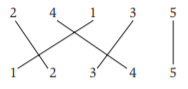
\includegraphics[width=0.25\textwidth]{Imagenes-Seccion5/fig5_4.PNG}
\caption{ Fig 5.4: Contando el número de inversiones en la secuencia 2, 4, 1, 3, 5. Cada par cruzado de segmentos de línea corresponde a un par que está en el orden opuesto en la lista de entrada y la lista ascendente, en otras palabras, una inversión.}
 \label{fig:Imagenes-Seccion5/fig5_4.PNG}
\end{wrapfigure}

Una forma natural de cuantificar esta noción es contar el número de inversiones. Decimos que dos índices $i<j$ forman una inversión si $a_i> a_j$, es decir, si los dos elementos $a_i$ y $a_j$ están "fuera de orden". Intentaremos determinar el número de inversiones en la secuencia $a_1, ... , u_n$.\\

Solo para precisar esta definición, considere un ejemplo en el que la secuencia es $2$, $4$, $1$, $3$, $5$. Hay tres inversiones en esta secuencia: $(2, 1), (4, 1) y (4, 3)$ ) También existe una forma geométrica atractiva de visualizar las inversiones, ilustrada en la figura 5.4: dibujamos la secuencia de los números ingresados ​​en el orden en que se proporcionan, y debajo de eso en orden ascendente. Luego dibujamos un segmento de línea entre cada número en la lista superior y su copia en la lista inferior. Cada par de segmentos de línea cruzados corresponde a un par que está en el orden opuesto en las dos listas; en otras palabras, una inversión.\\

Observe que el número de inversiones es una medida que interpola suavemente entre el acuerdo completo (cuando la secuencia está en orden ascendente, luego no hay inversiones) y el desacuerdo completo (si la secuencia está en orden descendente, entonces cada par forma una inversión, y entonces hay $n/2$ de ellos).\\

¿Cuál es el algoritmo más simple para contar las inversiones? Claramente, podríamos ver cada par de números $(a_i, a_j)$ y determinar si constituyen una inversión; esto tomaría el tiempo $O(n^2)$.\\

Ahora mostramos cómo contar el número de inversiones mucho más rápidamente, en el tiempo $O(nlogn)$. Tenga en cuenta que dado que puede haber un número cuadrático de inversiones, dicho algoritmo debe poder calcular el número total sin tener que mirar cada inversión individualmente. La idea básica es seguir la estrategia (†) definida en la Sección 5.1. Establecemos $m =\lceil n / 2 \rceil$  y divida la lista en las dos piezas $a_1, ..., a_m$ y $a_{m+1}, ..., a_n$. Primero contamos el número de inversiones en cada una de estas dos mitades por separado. Luego contamos el número de inversiones $(a_i, a_j)$, donde los dos números pertenecen a diferentes mitades; el truco es que debemos hacer esta parte en $O(n)$ tiempo, si queremos aplicar (5.2). Tenga en cuenta que estas inversiones de la primera mitad / segunda mitad tienen una forma particularmente agradable: son precisamente los pares $(a_i, a_j)$, donde ai está en la primera mitad, $a_j$ está en la segunda mitad y $a_i> a_j$.\\

Para ayudar a contar el número de inversiones entre las dos mitades, haremos que el algoritmo ordene recursivamente los números en las dos mitades también. Hacer que el paso recursivo haga un poco más de trabajo (ordenando así como contando las inversiones) hará que la porción de "combinación" del algoritmo sea más fácil\\

Entonces la rutina crucial en este proceso es Merge-and-Count. Supongamos que hemos ordenado recursivamente la primera y segunda mitad de la lista y contamos las inversiones en cada una. Ahora tenemos dos listas clasificadas A y B, que contienen la primera y la segunda mitades, respectivamente. Queremos producir una sola lista clasificada C de su unión, mientras también contamos el número de pares (a, b) con un $a \in A$, $b \in B$, y $a>b$. En nuestra discusión previa, esto es precisamente lo que necesitaremos para el paso de "combinación" que calcula el número de inversiones de la primera mitad / segunda mitad\\

Esto está estrechamente relacionado con el problema más simple que discutimos en el Capítulo 2, que formó el paso de "combinación" correspondiente para Mergesort: allí teníamos dos listas ordenadas A y B, y queríamos fusionarlas en una sola lista ordenada en $O(n)$ hora. La diferencia aquí es que queremos hacer algo extra: no solo deberíamos producir una sola lista ordenada de $A$ y $B$, sino que también deberíamos contar el número de "pares invertidos" $(a, b)$ donde $a \in A$, $b \in B$ y $a> b$.\\

Resulta que podremos hacer esto en el mismo estilo que utilizamos para la fusión. Nuestra rutina Merge-and-Count recorrerá las listas clasificadas $A$ y $B$, eliminando los elementos del frente y agregándolos a la lista ordenada $C$. En un paso dado, tenemos un puntero actual en cada lista, que muestra nuestra posición actual. Supongamos que estos indicadores están actualmente en los elementos $a_i$ y $b_j$. En un paso, comparamos los elementos $a_i$ y $b_j$ señalados en cada lista, eliminamos el más pequeño de su lista y lo agregamos al final de la lista $C$.\\

\begin{figure}[h]
\centering
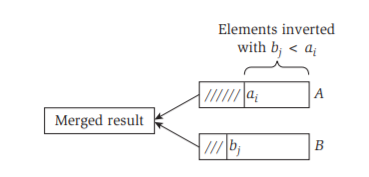
\includegraphics[scale=1.4]{Imagenes-Seccion5/fig5_5.PNG}
\caption{Figura 5.5 Fusionando dos listas ordenadas al mismo tiempo que se cuenta el número de inversiones entre ellas}
\end{figure}

Esto se encarga de la fusión. ¿Cómo también contamos el número de inversiones? Debido a que $A$ y $B$ están clasificados, en realidad es muy fácil hacer un seguimiento del número de inversiones que encontramos. Cada vez que se agrega el elemento $a_i$ a $C$, no se encuentran nuevas inversiones, ya que $a_i$ es más pequeño que todo lo que queda en la lista $B$, y viene antes que todas. Por otro lado, si $b_j$ se agrega a la lista $C$, entonces es más pequeño que todos los elementos restantes en $A$, y viene después de todos ellos, por lo que aumentamos nuestra cuenta del número de inversiones por la cantidad de elementos restantes en $A$. Esta es la idea crucial: en tiempo constante, hemos contabilizado un número potencialmente grande de inversiones. Vea la Figura 5.5 para una ilustración de este proceso\\

Para resumir, tenemos el siguiente algoritmo\\

\begin{lstlisting}
Fusionar y contar (A, B)
	Mantenga un puntero actual en cada lista, inicializado para indicar los elementos     		  frontales
    Mantener una variable Count para el numero de inversiones, 
        inicializado en 0
    Mientras ambas listas son no vacias:
        Establecer ai y bj sean los elementos indicados por el puntero actual
        Adjunte el mas chico de estos dos a la lista de salida
        Si bj es el elemento mas chico, entonces
            Incrementar Count por el numero de elementos restantes en A
        Fin si
        Avance el puntero actual en la lista desde la que se selecciono un elemento mas chico.
    Fin Mientras
    Una vez que una lista esta vacia, agregue el resto de la otra lista a la salida
    Retornar Count y la lista fusionada
\end{lstlisting}

El tiempo de ejecución de Merge-and-Count puede estar limitado por el análogo del argumento que usamos para el algoritmo de fusión original en el corazón de Mergesort: cada iteración del ciclo While toma tiempo constante, y en cada iteración agregamos algún elemento a la salida que nunca se volverá a ver. Por lo tanto, el número de iteraciones puede ser como máximo la suma de las longitudes iniciales de $A$ y $B$, por lo que el tiempo total de ejecución es $O (n)$.\\

Usamos esta rutina Merge-and-Count en un procedimiento recursivo que ordena y cuenta simultáneamente el número de inversiones en una lista L\\

\begin{lstlisting}
Ordenar_y_contar (L)
    Si la lista tiene un elemento, entonces
        no hay inversiones
    Sino
        Divida la lista en dos mitades:
        A contiene el primer $\lceil n/2 \rceil$  elementos
        B contiene los elementos $\lfloor n/2 \rfloor$ restantes
        (rA, A) = Ordenar_y_contar(A)
        (rB, B) = Ordenar_y_contar(B)
        (r, L) = Merge_y_contar(A, B)
    Fin si
    Devuelve r = rA + rB + r, y la lista ordenada L
\end{lstlisting}

Dado que nuestro procedimiento Merge-and-Count toma O (n) tiempo, el tiempo de ejecución T (n) del procedimiento completo Sort-and-Count satisface la recurrencia (5.1). Por (5.2), tenemos\\


\colorbox{mygray}{\parbox{15cm}{
\textbf{(5.7)} El algoritmo Sort-and-Count ordena correctamente la lista de entrada y cuenta el número de inversiones; se ejecuta en el tiempo $O (n log n)$ para una lista con n elementos.}}\\

\newpage

\section{Programación Dinámica}

Hemos visto que un algoritmo codicioso en particular produce una solución óptima para el problema de programación de intervalos, donde el objetivo es aceptar un conjunto tan grande de intervalos de superposición como sea posible. El problema de programación de intervalos ponderados es una versión estrictamente más general, en la que cada intervalo tiene un cierto valor (o peso), y queremos aceptar un conjunto de valores máximos.\\

\subsection{Diseñando un algoritmo recursivo}

Dado que el Problema de programación de intervalos original es simplemente el caso especial en el que todos los valores son iguales a 1, ya sabemos que la mayoría de los algoritmos codiciosos no resolverán este problema de manera óptima. Pero incluso el algoritmo que funcionó antes (elegir repetidamente el intervalo que termina antes) ya no es óptimo en esta configuración más general, como lo muestra el ejemplo simple en la Figura 6.1.\\

De hecho, no se conoce ningún algoritmo codicioso natural para este problema, que es lo que motiva nuestro cambio a la programación dinámica. Como se mencionó anteriormente, comenzaremos nuestra introducción a la programación dinámica con un tipo de algoritmo recursivo para este problema, y luego en la siguiente sección pasaremos a un método más iterativo que se acerca al estilo que utilizamos en el resto de este capítulo.\\

\begin{figure}[h]
\centering
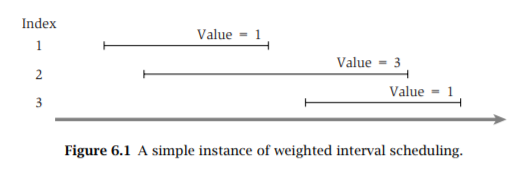
\includegraphics[scale=1]{Imagenes-Seccion6/fig6_1.PNG}
\caption{Figura 6.1 Una instancia simple de la programación de intervalos ponderados.}
\end{figure}

Usamos la notación de nuestra discusión de Programación de intervalos en la Sección 1.2. Tenemos n solicitudes etiquetadas 1,. . . , n, con cada solicitud i especificando una hora de inicio si y una hora de finalización fi. Cada intervalo i ahora también tiene un valor, o peso vi. Dos intervalos son compatibles si no se superponen. El objetivo de nuestro problema actual es seleccionar un subconjunto S ⊆ {1,. . . , n} de intervalos mutuamente compatibles, para maximizar la suma de los valores de los intervalos seleccionados,? $i \in S vi$.\\

Supongamos que las solicitudes se ordenan en orden de no finalización: f1 ≤ f2 ≤ ... ≤ fn. Diremos una solicitud i viene antes que una j si i <j. Este será el orden natural de izquierda a derecha en el que consideraremos los intervalos. Para ayudar a hablar sobre este orden, definimos p (j), para un intervalo j, para que sea el índice más grande i <j, de tal manera que los intervalos i y j estén separados. En otras palabras, i es el intervalo más a la izquierda que termina antes de que comience j. Definimos p (j) = 0 si ninguna solicitud i <j está separada de j. Un ejemplo de la definición de p (j) se muestra en la Figura 6.2.\\

Ahora, dada una instancia del problema de programación de intervalos ponderados, consideremos una solución óptima O, ignorando por ahora que no tenemos idea de lo que es. Aquí hay algo completamente obvio que podemos decir acerca de O: el intervalo n (el último) pertenece a O, o no lo hace. Supongamos que exploramos ambos lados de esta dicotomía un poco más lejos. Si $n  \in  O$, entonces claramente no hay intervalo indexado estrictamente entre p (n) yn puede pertenecer a O, porque según la definición de p (n), sabemos que los intervalos p (n) + 1, p (n) + 2 ,. . . , n - 1 todos los intervalos de superposición n. Además, si $n  \in  O$, entonces O debe incluir una solución óptima al problema que consiste en las solicitudes {1,. . . , p (n)}: si no fuera así, podríamos reemplazar la selección de solicitudes de O de {1,. . . , p (n)} con una mejor, sin peligro de
solicitud superpuesta n.\\

\begin{figure}[h]
\centering
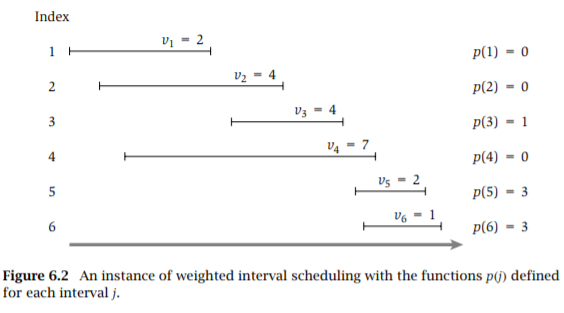
\includegraphics[scale=1]{Imagenes-Seccion6/fig6_2.PNG}
\caption{Figura 6.2 Una instancia de la programación de intervalos ponderados con las funciones p (j) definidas para cada intervalo j.}
\end{figure}

Por otro lado, si $n \not  \in  O$, entonces O es simplemente igual a la solución óptima al problema que consiste en las solicitudes {1,. . . , n - 1}. Esto es por un razonamiento completamente análogo: suponemos que O no incluye la solicitud n; así que si no elige el conjunto óptimo de solicitudes de {1,. . . , n - 1}, podríamos reemplazarlo por uno mejor.\\

Todo esto sugiere que encontrar la solución óptima en intervalos {1, 2,. . . , n} implica observar las soluciones óptimas de problemas más pequeños de la forma {1, 2,. . . , j}. Por lo tanto, para cualquier valor de j entre 1 y n, permita que Oj denote la solución óptima al problema que consiste en las solicitudes {1,. . . , j}, y deje que OPT (j) denote el valor de esta solución. (Definimos OPT (0) = 0, según la convención de que este es el óptimo en un conjunto vacío de intervalos). La solución óptima que estamos buscando es precisamente On, con el valor OPT (n). Para la solución óptima Oj en {1, 2,. . . , j}, nuestro razonamiento anterior (generalizando desde el caso en el que j = n) dice que o $j  \in  Oj$, en cuyo caso OPT (j) = vj + OPT (p (j)), o j? Oj, en en qué caso OPT (j) = OPT (j - 1). Dado que estas son precisamente las dos opciones posibles ($j  \in  Oj o j?  \in  Oj$), podemos decir además que\\


\colorbox{mygray}{\parbox{15cm}{
\textbf{(6.1)} OPT(j) = max(vj + OPT(p(j)), OPT(j − 1))}}\\

¿Y cómo decidimos si n pertenece a la solución óptima Oj? Esto también es fácil: pertenece a la solución óptima si y solo si la primera de las opciones anteriores es al menos tan buena como la segunda; en otras palabras,\\

\colorbox{mygray}{\parbox{15cm}{
\textbf{(6.2)} La solicitud j pertenece a una solución óptima en el conjunto {1, 2,. . . , j} si y solo si
vj + OPT(p(j)) ≥ OPT(j − 1).
}}\\

Estos hechos forman el primer componente crucial en el que se basa una solución de programación dinámica: una ecuación de recurrencia que expresa la solución óptima (o su valor) en términos de las soluciones óptimas para subproblemas más pequeños. A pesar del simple razonamiento que llevó a este punto, (6.1) ya es un desarrollo significativo. Nos da directamente un algoritmo recursivo para calcular OPT (n), asumiendo que ya hemos ordenado las solicitudes por tiempo de finalización y computamos los valores de p (j) para cada j.\\

\begin{figure}[h]
\centering
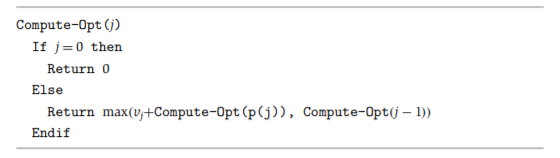
\includegraphics[scale=1.2]{Imagenes-Seccion6/cod6_1.PNG}
\end{figure}

La corrección del algoritmo sigue directamente por inducción en j:

\colorbox{mygray}{\parbox{15cm}{
\textbf{(6.3)} Compute-Opt (j) calcula correctamente OPT (j) para cada j = 1, 2,. . . , n.}}\\

Prueba. Por definición, OPT (0) = 0. Ahora, tome algo de j> 0, y suponga, a modo de inducción, que Compute-Opt (i) calcula correctamente OPT (i) para todos i <j. Por la hipótesis de la inducción, sabemos que Compute-Opt (p (j)) = OPT (p (j)) y Compute-Opt (j - 1) = OPT (j - 1); y por lo tanto de (6.1) se deduce que\\

OPT(j) = max(vj + Compute-Opt(p(j)), Compute-Opt(j − 1))
= Compute-Opt(j).

Desafortunadamente, si realmente implementamos el algoritmo Compute-Opt como se acaba de escribir, tomaría un tiempo exponencial para ejecutarse en el peor de los casos. Por ejemplo, consulte la Figura 6.3 para ver el árbol de llamadas emitidas para la instancia de la Figura 6.2: el árbol se ensancha muy rápidamente debido a la ramificación recursiva. Para tomar un ejemplo más extremo, en una instancia muy bien en capas como la de la Figura 6.4, donde p (j) = j - 2 para cada j = 2, 3, 4,. . . , n, vemos que Compute-Opt (j) genera llamadas recursivas separadas en problemas de tamaños j - 1 y j - 2. En otras palabras, el número total de llamadas hechas a Compute-Opt en esta instancia aumentará\\

\begin{figure}[h]
\centering
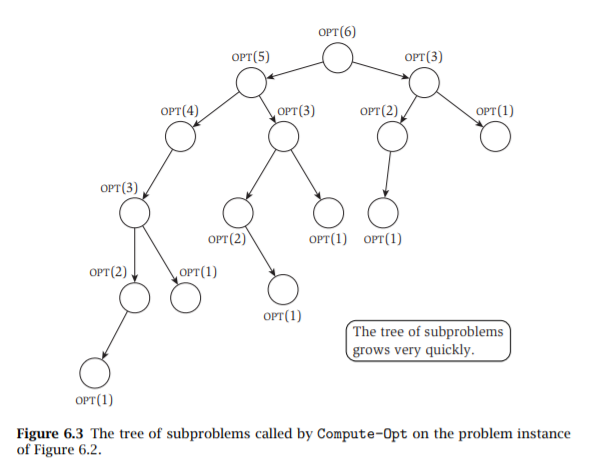
\includegraphics[scale=1]{Imagenes-Seccion6/fig6_3.PNG}
\caption{Figura 6.3 El árbol de subproblemas llamado por Compute-Opt en la instancia de problema de la Figura 6.2.}
\end{figure}


\begin{figure}[h]
\centering
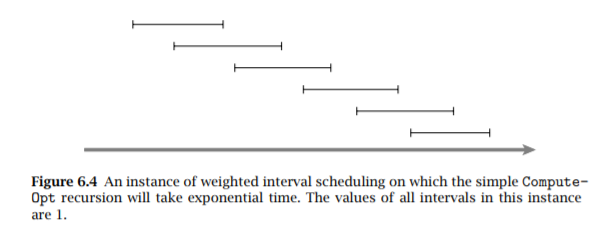
\includegraphics[scale=1.2]{Imagenes-Seccion6/fig6_4.PNG}
\caption{Figura 6.4 Una instancia de la programación de intervalos ponderados en la que la recursión ComputeOpt simple tomará tiempo exponencial. Los valores de todos los intervalos en este caso son 1.}
\end{figure}

Al igual que los números de Fibonacci, que aumentan exponencialmente. Por lo tanto, no hemos logrado una solución de tiempo polinomial.\\


\subsection{Memorizando la recursion}

De hecho, sin embargo, no estamos tan lejos de tener un algoritmo de tiempo polinomial. Una observación fundamental, que forma el segundo componente crucial de una solución de programación dinámica, es que nuestro algoritmo recursivo ComputeOpt en realidad solo resuelve n + 1 subproblemas diferentes: Compute-Opt (0), Compute-Opt (1), ..., Compute-Opt (n). El hecho de que se ejecute en tiempo exponencial como está escrito se debe simplemente a la espectacular redundancia en el número de veces que emite cada una de estas llamadas.\\

¿Cómo podríamos eliminar toda esta redundancia? Podríamos almacenar el valor de Compute-Opt en un lugar accesible globalmente la primera vez que lo computamos y luego simplemente usar este valor precomputado en lugar de todas las llamadas recursivas futuras. Esta técnica de guardar valores que ya se han calculado se denomina memorización.\\

Implementamos la estrategia anterior en el procedimiento más "inteligente" MCompute-Opt. Este procedimiento hará uso de una matriz M [0. . . norte]; M [j] comenzará con el valor "vacío", pero mantendrá el valor de Compute-Opt (j) tan pronto como se determine por primera vez. Para determinar OPT (n), invocamos M-ComputeOpt (n).\\


\begin{figure}[h]
\centering
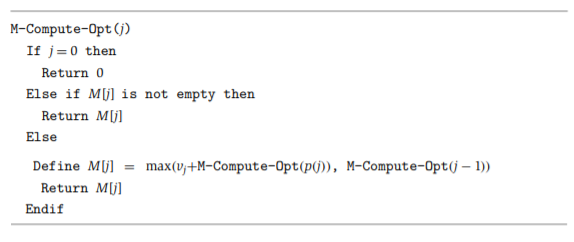
\includegraphics[scale=1]{Imagenes-Seccion6/cod6_2.PNG}
\end{figure}

\subsubsection*{Analizando la versión memorizada}

Claramente, esto se ve muy similar a nuestra implementación previa del algoritmo; Sin embargo, la memoria ha reducido el tiempo de ejecución.


\colorbox{mygray}{\parbox{15cm}{
\textbf{(6.4)} El tiempo de ejecución de M-Compute-Opt (n) es O (n) (suponiendo que los intervalos de entrada están ordenados por sus tiempos de finalización).}}\\

Prueba. El tiempo empleado en una sola llamada a M-Compute-Opt es O (1), excluyendo el tiempo empleado en las llamadas recursivas que genera. Por lo tanto, el tiempo de ejecución está limitado por una cantidad constante de veces el número de llamadas emitidas a M-Compute-Opt. Dado que la implementación en sí misma no proporciona un límite superior explícito en este número de llamadas, intentamos encontrar un límite buscando una buena medida del "progreso".\\

La medida de progreso más útil aquí es el número de entradas en M que no están "vacías". Inicialmente, este número es 0; pero cada vez que el procedimiento invoca la repetición, emite dos llamadas recursivas a M-Compute-Opt, llena una nueva entrada y, por lo tanto, aumenta el número de entradas completadas en 1. Ya que M tiene solo n + 1 entradas, sigue que puede haber, como máximo, llamadas O (n) a M-ComputeOpt y, por lo tanto, el tiempo de ejecución de M-Compute-Opt (n) es O (n), según se desee.\\

\subsubsection*{Calcular una solución además de su valor}

Hasta ahora, simplemente hemos calculado el valor de una solución óptima; Presumiblemente también queremos un conjunto óptimo de intervalos. Sería fácil extender M-Compute-Opt para seguir la pista de una solución óptima además de su valor: podríamos mantener una matriz S adicional para que S [i] contenga un conjunto óptimo de intervalos entre {1, 2 ,. . . , yo}. Sin embargo, la mejora ingenua del código para mantener las soluciones en la matriz S aumentaría el tiempo de ejecución por un factor adicional de O (n): mientras que una posición en la matriz M se puede actualizar en tiempo O (1), anotando un conjunto en la matriz S lleva tiempo O (n). Podemos evitar este estallido O (n) no manteniendo S explícitamente, sino recuperando la solución óptima de los valores guardados en la matriz M después de que se haya calculado el valor óptimo.\\

Sabemos por (6.2) que j pertenece a una solución óptima para el conjunto de intervalos {1,. . . , j} si y solo si vj + OPT (p (j)) ≥ OPT (j - 1). Usando esta observación, obtenemos el siguiente procedimiento simple, que "rastrea" a través de la matriz M para encontrar el conjunto de intervalos en una solución óptima.\\

COD6 3.PNG

Como Find-Solution se llama a sí mismo recursivamente solo en valores estrictamente más pequeños, hace un total de O (n) llamadas recursivas; y como pasa un tiempo constante por llamada, tenemos\\

\colorbox{mygray}{\parbox{15cm}{
\textbf{(6.5)} Dada la matriz M de los valores óptimos de los subproblemas, FindSolution devuelve una solución óptima en tiempo O (n).}}\\

\subsection{Principios de la Programación Dinámica: Memoización o Iteración sobre Subproblemas}

Ahora usamos el algoritmo para el problema de programación de intervalos ponderados desarrollado en la sección anterior para resumir los principios básicos de la programación dinámica, y también para ofrecer una perspectiva diferente que será fundamental para el resto del capítulo: iterar sobre los subproblemas, en lugar de computar Soluciones recursivas.\\

En la sección anterior, desarrollamos una solución de tiempo polinómico para el problema de programación de intervalos ponderados diseñando primero un algoritmo recursivo de tiempo exponencial y luego convirtiéndolo (por memoización) en un algoritmo recursivo eficiente que consultó una matriz global M de soluciones óptimas para subproblemas. Sin embargo, para comprender realmente lo que está sucediendo aquí, es útil formular una versión esencialmente equivalente del algoritmo. Es esta nueva formulación la que captura de manera más explícita la esencia de la técnica de programación dinámica, y servirá como una plantilla general para los algoritmos que desarrollamos en secciones posteriores.\\

\subsubsection*{Diseñando el algoritmo}

La clave para el algoritmo eficiente es realmente la matriz M. Codifica la noción de que estamos usando el valor de soluciones óptimas para los subproblemas en intervalos {1, 2,. . . , j} para cada j, y usa (6.1) para definir el valor de M [j] en función de los valores que vienen antes en la matriz. Una vez que tenemos la matriz M, el problema se resuelve: M [n] contiene el valor de la solución óptima en la instancia completa, y Find-Solution se puede usar para rastrear a través de M de manera eficiente y devolver la solución óptima.\\

El punto a tener en cuenta, entonces, es que podemos calcular directamente las entradas en M mediante un algoritmo iterativo, en lugar de usar la recursión memorizada. Simplemente comenzamos con M [0] = 0 y seguimos incrementando j; Cada vez que necesitamos determinar un valor M [j], la respuesta es proporcionada por (6.1). El algoritmo se ve como sigue.\\

COD6 4.PNG

\subsubsection*{Analizando el algoritmo}

Por analogía exacta con la prueba de (6.3), podemos probar por inducción en j que este algoritmo escribe OPT (j) en la entrada de matriz M [j]; (6.1) proporciona el paso de inducción. Además, como antes, podemos pasar la matriz M llena a Find-Solution para obtener una solución óptima además del valor. Finalmente, el tiempo de ejecución de Iterative-Compute-Opt es claramente O (n), ya que se ejecuta explícitamente para n iteraciones y pasa un tiempo constante en cada una.\\

En la Figura 6.5 se muestra un ejemplo de la ejecución de Iterative-Compute-Opt. En cada iteración, el algoritmo completa una entrada adicional de la matriz M, comparando el valor de vj + M [p (j)] con el valor de M [j - 1].\\

\subsubsection*{Un esquema básico de programación dinámica}

Esto, entonces, proporciona un segundo algoritmo eficiente para resolver el problema de programación de intervalos ponderados. Los dos enfoques claramente tienen una gran coincidencia conceptual, ya que ambos crecen a partir de la percepción contenida en la recurrencia (6.1). Para el resto del capítulo, desarrollaremos algoritmos de programación dinámica utilizando el segundo tipo de enfoque, la construcción iterativa de subproblemas, porque los algoritmos suelen ser más sencillos de expresar de esta manera. Pero en cada caso que consideramos, hay una manera equivalente de formular el algoritmo como una recursión memorizada.\\

Lo más importante es que la mayor parte de nuestra discusión sobre el problema particular de la selección de intervalos se puede proyectar más generalmente como una plantilla aproximada para diseñar algoritmos de programación dinámica. Para comenzar a desarrollar un algoritmo basado en la programación dinámica, se necesita una colección de subproblemas derivados del problema original que satisfaga algunas propiedades básicas\\

\begin{figure}[h]
\centering
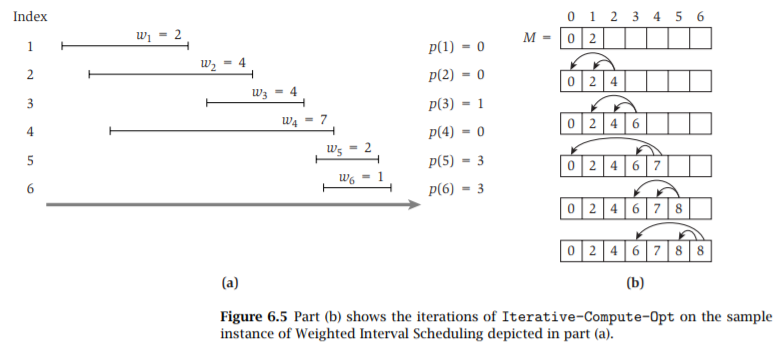
\includegraphics[scale=0.8]{Imagenes-Seccion6/fig6_5.PNG}
\caption{Figura 6.5 La parte (b) muestra las iteraciones de Iterative-Compute-Opt en la instancia de muestra de la Programación de intervalos ponderados representada en la parte (a).}
\end{figure}

\begin{itemize}

    \item Solo hay un número polinomial de subproblemas.

    \item La solución al problema original se puede calcular fácilmente de las soluciones a los subproblemas. (Por ejemplo, el problema original puede ser uno de los subproblemas).
    
    \item Hay un orden natural en los subproblemas desde "más pequeño" a "más grande", junto con una recurrencia fácil de calcular (como en (6.1) y (6.2)) que permite determinar la solución a un subproblema desde Las soluciones a algunos subproblemas más pequeños.

\end{itemize}

Naturalmente, estas son pautas informales. En particular, la noción de "más pequeño" en la parte (iii) dependerá del tipo de recurrencia que se tenga.\\

Veremos que a veces es más fácil iniciar el proceso de diseño de tal algoritmo mediante la formulación de un conjunto de subproblemas que parecen naturales y luego descubrir una recurrencia que los vincule entre sí; pero a menudo (como sucedió en el caso de la planificación de intervalos ponderados), puede ser útil definir primero una recurrencia razonando acerca de la estructura de una solución óptima, y ​​luego determinar qué subproblemas serán necesarios para desenrollar la recurrencia. Esta relación de gallina y huevo entre los subproblemas y las recurrencias es un problema sutil que subyace a la programación dinámica. Nunca está claro que una colección de subproblemas será útil hasta que uno encuentre una recurrencia que los vincule; pero puede ser difícil pensar en las recurrencias en ausencia de los subproblemas "más pequeños" sobre los que se basan. En las secciones posteriores, desarrollaremos una mayor práctica en la gestión de este compromiso de diseño.\\

\subsection{Mínimos cuadrados segmentados: opciones de múltiples vías}

Ahora analizamos un tipo diferente de problema, que ilustra un estilo de programación dinámica ligeramente más complicado. En la sección anterior, desarrollamos una recurrencia basada en una elección fundamentalmente binaria: o el intervalo n pertenecía a una solución óptima o no. En el problema que consideramos aquí, la recurrencia implicará lo que podría llamarse "opciones de múltiples vías": en cada paso, tenemos un número polinomial de posibilidades a considerar para la estructura de la solución óptima. Como veremos, el enfoque de programación dinámica se adapta a esta situación más general de manera muy natural.\\

Como un tema aparte, el problema desarrollado en esta sección también es una buena ilustración de cómo una definición algorítmica limpia puede formalizar una noción que inicialmente parece demasiado difusa y no intuitiva para trabajar matemáticamente.\\


\subsubsection*{El problema}

A menudo, al observar datos científicos o estadísticos, representados en un conjunto de ejes bidimensional, se intenta pasar una "línea de mejor ajuste" a través de los datos, como se muestra en la Figura 6.6.\\

Este es un problema fundamental en estadística y análisis numérico, formulado de la siguiente manera. Supongamos que nuestros datos consisten en un conjunto P de n puntos en el plano, denotado (x1, y1), (x2, y2), ..., (xn, yn); y supongamos x1 <x2 <... <xn. Dada una línea L definida por la ecuación y = ax + b, decimos que el error de L con respecto a P es la suma de sus “distancias” cuadradas a los puntos en P:\\

\begin{figure}[h]
\centering
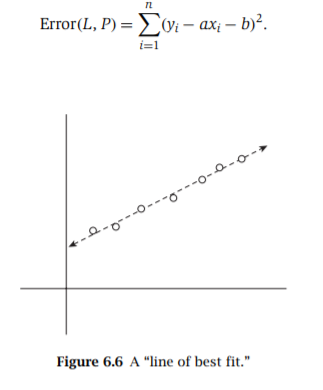
\includegraphics[scale=1]{Imagenes-Seccion6/fig6_6.PNG}
\caption{Figura 6.6 Una "línea de mejor ajuste".}
\end{figure}

\begin{figure}[h]
\centering
\includegraphics[scale=1]{Imagenes-Seccion6/fig6_7.PNG}
\caption{Figura 6.7 Un conjunto de puntos que se encuentran aproximadamente en dos líneas.}
\end{figure}

Un objetivo natural es entonces encontrar la línea con el mínimo error; esto resulta tener una buena solución de forma cerrada que se puede derivar fácilmente usando el cálculo. Al omitir la derivación aquí, simplemente indicamos el resultado: la línea de error mínimo es y = ax + b, donde


\begin{figure}[h]
\centering
\includegraphics[scale=1]{Imagenes-Seccion6/cod6_1.PNG}
\end{figure}

Ahora, aquí hay un tipo de problema que estas fórmulas no fueron diseñadas para cubrir. A menudo tenemos datos que se parecen en algo a la imagen de la Figura 6.7. En este caso, nos gustaría hacer una afirmación como: "Los puntos se encuentran aproximadamente en una secuencia de dos líneas". ¿Cómo podríamos formalizar este concepto?\\

Esencialmente, cualquier línea simple a través de los puntos en la figura tendría un error terrible; pero si usamos dos líneas, podríamos lograr un error bastante pequeño. Por lo tanto, podemos intentar formular un nuevo problema de la siguiente manera: en lugar de buscar una línea de mejor ajuste, se nos permite pasar un conjunto arbitrario de líneas a través de los puntos, y buscamos un conjunto de líneas que minimice el error. Pero esto falla como una buena formulación de problemas, porque tiene una solución trivial: si se nos permite ajustar los puntos con un conjunto de líneas arbitrariamente grande, podríamos ajustar los puntos perfectamente haciendo que una línea diferente pase a través de cada par de líneas consecutivas. puntos en P.\\

En el otro extremo, podríamos intentar "codificar" el número dos en el problema; Podríamos buscar el mejor ajuste usando a lo sumo dos líneas. Pero esto también pierde una característica crucial de nuestra intuición: no comenzamos con una idea preconcebida de que los puntos se encuentran aproximadamente en dos líneas; Llegamos a la conclusión de que al mirar la foto. Por ejemplo, la mayoría de las personas diría que los puntos en la Figura 6.8 se encuentran aproximadamente en tres líneas.\\

\begin{figure}[h]
\centering
\includegraphics[scale=1]{Imagenes-Seccion6/fig6_8.PNG}
\caption{Figura 6.8 Un conjunto de puntos que se encuentran aproximadamente en tres líneas.}
\end{figure}

Por lo tanto, de manera intuitiva, necesitamos una formulación de problemas que nos obligue a ajustar los puntos bien, utilizando el menor número de líneas posible. Ahora formulamos un problema, el problema de mínimos cuadrados segmentados, que captura estos problemas de manera bastante limpia. El problema es una instancia fundamental de un problema en la minería de datos y las estadísticas conocidas como detección de cambios: dada una secuencia de puntos de datos, queremos identificar algunos puntos en la secuencia en los que se produce un cambio discreto (en este caso, un cambio de una aproximación lineal a otra).\\

Formulando el problema Como en la discusión anterior, se nos da un conjunto de puntos P = {(x1, y1), (x2, y2), ..., (xn, yn)}, con x1 <x2 <... <xn. Usaremos pi para denotar el punto (xi, yi). Primero debemos dividir P en un número de segmentos. Cada segmento es un subconjunto de P que representa un conjunto contiguo de coordenadas x; es decir, es un subconjunto de la forma {pi, pi + 1, ..., pj − 1, pj} para algunos índices i ≤ j. Luego, para cada segmento S en nuestra partición de P, calculamos la línea minimizando el error con respecto a los puntos en S, de acuerdo con las fórmulas anteriores.\\

La penalización de una partición se define como una suma de los siguientes términos.\\

\begin{itemize}
    \item El número de segmentos en los que particionamos P, multiplicado por un multiplicador dado C> 0.
    \item Para cada segmento, el valor de error de la línea óptima a través de ese segmento.
\end{itemize}

Nuestro objetivo en el problema de mínimos cuadrados segmentados es encontrar una partición de la penalización mínima. Esta minimización captura los compromisos que discutimos anteriormente. Se nos permite considerar las particiones en cualquier número de segmentos; a medida que aumentamos el número de segmentos, reducimos los términos de penalización en la parte (ii) de la definición, pero aumentamos el término en la parte (i). (El multiplicador C se proporciona con la entrada, y al sintonizar C, podemos penalizar el uso de líneas adicionales en mayor o menor medida).\\

Existen exponencialmente muchas particiones posibles de P, e inicialmente no está claro que debamos poder encontrar la óptima de manera eficiente. Ahora mostramos cómo usar la programación dinámica para encontrar una partición con una penalización mínima en el polinomio de tiempo en n.\\

\subsubsection*{Diseñando el algoritmo}

Para empezar, debemos recordar los ingredientes que necesitamos para un algoritmo de programación dinámico, como se describe al final de la Sección 6.2. Queremos un número polinomial de subproblemas, cuyas soluciones deberían brindar una solución al problema original; y deberíamos poder crear soluciones para estos subproblemas usando una recurrencia. Al igual que con el problema de programación de intervalos ponderados, es útil pensar en algunas propiedades simples de la solución óptima. Tenga en cuenta, sin embargo, que en realidad no existe una analogía directa con la planificación de intervalos ponderados: allí buscábamos un subconjunto de n objetos, mientras que aquí buscamos particionar n objetos.\\

Para los mínimos cuadrados segmentados, la siguiente observación es muy útil: el último punto pn pertenece a un solo segmento en la partición óptima, y ​​ese segmento comienza en algún punto anterior pi. Este es el tipo de observación que puede sugerir el conjunto correcto de subproblemas: si conociéramos la identidad del último segmento pi, ..., pn (ver Figura 6.9), podríamos eliminar esos puntos de la consideración y resolver el problema recursivamente en los puntos restantes p1, ..., pi − 1.\\


\begin{figure}
\includegraphics[scale=1.0]{Imagenes-Seccion6/fig6_9.PNG}
\caption{\label{Figura 6.9} Una posible solución: un solo segmento de línea se ajusta a los puntos pi, pi + 1, ..., pn, y luego se encuentra una solución óptima para los puntos restantes p1, p2, ..., pi − 1.}
\end{figure}

Supongamos que dejamos que OPT (i) denote la solución óptima para los puntos p1, ..., pi, y dejamos que ei, j denote el error mínimo de cualquier línea con respecto a pi, pi + 1, ..., pj. (Escribiremos OPT (0) = 0 como un caso de límite). Luego, nuestra observación anterior dice lo siguiente.\\

\colorbox{mygray}{\parbox{15cm}{
\textbf{(6.6)} Si el último segmento de la partición óptima es pi, ..., pn, entonces el valor de la solución óptima es OPT (n) = ei, n + C + OPT (i - 1).}}\\

Usando la misma observación para el subproblema que consiste en los puntos p1, ..., pj, vemos que para obtener OPT (j) debemos encontrar la mejor manera de producir un segmento final pi, ..., pj: pagar el error más un C adicional para este segmento, junto con una solución óptima OPT (i - 1) para los puntos restantes. En otras palabras, hemos justificado la siguiente recurrencia.\\

\colorbox{mygray}{\parbox{15cm}{
\textbf{(6.7)} Para el subproblema en los puntos p1, ..., pj, OPT (j) = min 1≤i≤j (ei, j + C + OPT (i - 1)), y el segmento pi, .. ., pj se usa en una solución óptima para el subproblema si y solo si el mínimo se obtiene usando el índice i.}}\\

La parte difícil en el diseño del algoritmo ahora está detrás de nosotros. A partir de aquí, simplemente construimos las soluciones OPT (i) para aumentar i.

\begin{figure}[h]
\centering
\includegraphics[scale=1]{Imagenes-Seccion6/cod6_5.PNG}
\end{figure}

Por analogía con los argumentos para la programación de intervalos ponderados, la exactitud de este algoritmo se puede probar directamente por inducción, con (6.7) proporcionando el paso de inducción.\\

Y como en nuestro algoritmo para la programación de intervalos ponderados, podemos rastrear a través de la matriz M para calcular una partición óptima.\\

\begin{figure}[h]
\centering
\includegraphics[scale=1]{Imagenes-Seccion6/cod6_6.PNG}
\end{figure}

\subsubsection*{Analizando el algoritmo}

Finalmente, consideramos el tiempo de ejecución de los mínimos cuadrados segmentados. Primero debemos calcular los valores de todos los errores de mínimos cuadrados ei, j. Para realizar una contabilidad simple del tiempo de ejecución para esto, notamos que hay O (n2) pares (i, j) para los cuales se necesita este cálculo; y para cada par (i, j), podemos usar la fórmula dada al principio de esta sección para calcular ei, j en tiempo O (n). Por lo tanto, el tiempo total de ejecución para calcular todos los valores de ei, j es O (n3).\\

Siguiendo esto, el algoritmo tiene n iteraciones, para valores j = 1,. . . , n. Para cada valor de j, tenemos que determinar el mínimo en la recurrencia (6.7) para completar la entrada de la matriz M [j]; esto toma tiempo O (n) para cada j, para un total de O (n2). Por lo tanto, el tiempo de ejecución es O (n2) una vez que se han determinado todos los valores ei, j.\\

\subsection{El problema de la mochila: Agregar una variable}

Estamos viendo cada vez más que los problemas en la programación proporcionan una fuente rica de problemas algorítmicos motivados en la práctica. Hasta ahora hemos considerado problemas en los que las solicitudes se especifican por un intervalo de tiempo dado en un recurso, así como problemas en los que las solicitudes tienen una duración y una fecha límite, pero no requieren un intervalo en particular durante el cual deben realizarse.\footnote{1 En este análisis, el tiempo de ejecución está dominado por la O (n3) necesaria para calcular todos los valores ei, j. Pero, de hecho, es posible calcular todos estos valores en tiempo O (n2), lo que reduce el tiempo de ejecución del algoritmo completo a O (n2). La idea, cuyos detalles dejaremos como ejercicio para el lector, es primero calcular ei, j para todos los pares (i, j) donde j - i = 1, luego para todos los pares donde j - i = 2, luego j - i = 3, y así sucesivamente. De esta manera, cuando llegamos a un valor ei, j particular, podemos usar los ingredientes del cálculo
para ei, j − 1 para determinar ei, j en tiempo constante.}\\

En esta sección, consideramos una versión del segundo tipo de problema, con duraciones y plazos, que es difícil de resolver directamente utilizando las técnicas que hemos visto hasta ahora. Usaremos la programación dinámica para resolver el problema, pero con un giro: el conjunto "obvio" de subproblemas resultará no ser suficiente, por lo que terminamos creando una colección más rica de subproblemas. Como veremos, esto se hace agregando una nueva variable a la recurrencia subyacente al programa dinámico.\\

\subsubsection*{El problema}

En el problema de programación que consideramos aquí, tenemos una sola máquina que puede procesar trabajos, y tenemos un conjunto de solicitudes {1, 2,. . . , n}. Solo podemos usar este recurso durante el período comprendido entre el tiempo 0 y el tiempo W, para un número W. Cada solicitud corresponde a un trabajo que requiere tiempo para procesar. Si nuestro objetivo es procesar trabajos para mantener la máquina lo más ocupada posible hasta el "corte" W, ¿qué trabajos debemos elegir?\\

Más formalmente, nos dan n artículos {1,. . . , n}, y cada uno tiene un peso no negativo dado wi (para i = 1, ..., n). También se nos da un límite W. Nos gustaría seleccionar un subconjunto S de los elementos para que? i wS wi ≤ W y, sujeto a esta restricción,? i wS wi es lo más grande posible. Llamaremos a esto el problema de suma de subconjuntos.\\

Este problema es un caso especial natural de un problema más general llamado el Problema de la mochila, donde cada solicitud i tiene un valor vi y un peso wi. El objetivo de este problema más general es seleccionar un subconjunto del valor total máximo, sujeto a la restricción de que su peso total no exceda a W. Los problemas de mochila a menudo aparecen como subproblemas en otros problemas más complejos. El nombre de mochila se refiere al problema de llenar una mochila de capacidad W lo más llena posible (o empaquetar con el mayor valor posible), utilizando un subconjunto de los elementos {1,. . . , n}. Usaremos peso o tiempo al referirnos a las cantidades wi y W.\\

Como esto se asemeja a otros problemas de programación que hemos visto antes, es natural preguntar si un algoritmo codicioso puede encontrar la solución óptima. Parece que la respuesta es no, al menos no se conoce una regla codiciosa eficiente que siempre construya una solución óptima. Un enfoque codicioso natural sería intentar clasificar los artículos disminuyendo el peso, o al menos hacer esto para todos los elementos de peso a lo sumo de W, y luego comenzar a seleccionar los artículos en este orden siempre que el peso total permanezca por debajo de W. Pero si W es un múltiplo de 2, y tenemos tres elementos con ponderaciones {W / 2 + 1, W / 2, W / 2}, vemos que este algoritmo codicioso no producirá la solución óptima. Alternativamente, podríamos clasificar aumentando el peso y luego hacer lo mismo; pero esto falla en entradas como {1, W / 2, W / 2}.\\

El objetivo de esta sección es mostrar cómo usar la programación dinámica para resolver este problema. Recuerde los principios principales de la programación dinámica: tenemos que crear un pequeño número de subproblemas para que cada subproblema pueda resolverse fácilmente a partir de subproblemas "más pequeños", y la solución al problema original se puede obtener fácilmente una vez que sepamos las soluciones para Todos los subproblemas. El problema difícil aquí radica en descubrir un buen conjunto de subproblemas.\\

\subsubsection*{Diseñando el algoritmo}

\textbf{Un comienzo falso} Una estrategia general, que funcionó para nosotros en el caso de la Programación de intervalos ponderados, es considerar los subproblemas que involucran solo las primeras solicitudes i. Comenzamos probando esta estrategia aquí. Usamos la notación OPT (i), análogamente a la notación usada antes, para denotar la mejor solución posible utilizando un subconjunto de las solicitudes {1,. . . , yo}. La clave de nuestro método para el problema de programación de intervalos ponderados fue concentrarse en una solución óptima O a nuestro problema y considerar dos casos, dependiendo de si la última solicitud n es aceptada o rechazada por esta solución óptima. Al igual que en ese caso, tenemos la primera parte, que sigue inmediatamente a la definición de OPT (i).\\

. Si $n \not  \in  O$, entonces OPT (n) = OPT (n - 1).\\

A continuación, debemos considerar el caso en el que $n  \in  O$. Lo que nos gustaría aquí es una simple recursión, que nos indica el mejor valor posible que podemos obtener para las soluciones que contienen la última solicitud n. Para la Programación de intervalos ponderados, esto fue fácil, ya que simplemente podríamos eliminar cada solicitud que estuviera en conflicto con la solicitud n. En el problema actual, esto no es tan simple. Aceptar la solicitud n no implica de manera inmediata que tenemos que rechazar cualquier otra solicitud. En cambio, significa que para el subconjunto de solicitudes S ⊆ {1,. . . , n - 1} que aceptaremos, nos queda menos peso disponible: se utiliza un peso de wn en la solicitud aceptada n, y solo nos queda un peso W - wn para el conjunto S de solicitudes restantes que aceptamos. Vea la Figura 6.10.\\

\textbf{Una solución mejor} Esto sugiere que necesitamos más subproblemas: para averiguar el valor de OPT (n) no solo necesitamos el valor de OPT (n - 1), sino que también necesitamos saber la mejor solución que podemos obtener utilizando un subconjunto de los primeros n - 1 artículos y peso total permitido W - wn. Por lo tanto, vamos a utilizar muchos más subproblemas: uno para cada conjunto inicial {1,. . . , i} de los artículos, y cada valor posible para el peso disponible restante w. Supongamos que W es un número entero, y todas las solicitudes i = 1,. . . , n tienen pesos enteros wi. Tendremos un subproblema para cada i = 0, 1,. . . , ny cada entero 0 ≤ w ≤ W. Usaremos OPT (i, w) para indicar el valor de la solución óptima utilizando un subconjunto de los elementos {1,. . . , i} con el peso máximo permitido w, es decir, donde el máximo está sobre los subconjuntos S ⊆ {1,. . . , i} que satisfacen? $j \in S$ $wj ≤ w$. Usando este nuevo conjunto de subproblemas, podremos expresar el valor OPT (i, w) como una expresión simple en términos de valores de problemas más pequeños. Además, OPT (n, W) es la cantidad que estamos buscando al final. Como antes, deje que O denote una solución óptima para el problema original.\\


\begin{figure}[h]
\centering
\includegraphics[scale=1]{Imagenes-Seccion6/fig6_10.PNG}
\caption{Figura 6.10 Después de incluir el artículo n en la solución, se utiliza un peso de wn y queda W - wn de peso disponible.}
\end{figure}

$OPT(i,w) = \max_s \sum_{j \in S} w_j$\\

donde el máximo está sobre los subconjuntos S ⊆ {1,. . . , i} que satisfacen? $j \in S$ wj ≤ w. Usando este nuevo conjunto de subproblemas, podremos expresar el valor OPT (i, w) como una expresión simple en términos de valores de problemas más pequeños. Además, OPT (n, W) es la cantidad que estamos buscando al final. Como antes, deje que O denote una solución óptima para el problema original.\\

\begin{itemize}
    \item Si $n \not  \in  O$, entonces OPT (n, W) = OPT (n - 1, W), ya que simplemente podemos ignorar el elemento n
    \item Si $n  \in  O$, entonces OPT (n, W) = wn + OPT (n - 1, W - wn), ya que ahora buscamos utilizar la capacidad restante de W - wn de manera óptima en los elementos 1, 2,. . . , n - 1.
\end{itemize}

Cuando el enésimo artículo es demasiado grande, es decir, W <wn, entonces debemos tener OPT (n, W) = OPT (n - 1, W). De lo contrario, obtendremos la solución óptima permitiendo todas las n solicitudes al aprovechar estas dos opciones. Usando la misma línea de argumento para el subproblema para los elementos {1,. . . , i}, y el peso máximo permitido w, nos da la siguiente recurrencia.\\

\colorbox{mygray}{\parbox{15cm}{
\textbf{(6.8)} Si w < wi then OPT(i, w) = OPT(i − 1, w). Otro caso
OPT(i, w) = max(OPT(i − 1, w), wi + OPT(i − 1, w − wi)).}}\\\\

Como antes, queremos diseñar un algoritmo que construya una tabla de todos los valores OPT (i, w) mientras calculamos cada uno de ellos como máximo una vez.

\begin{figure}[h]
\centering
\includegraphics[scale=1]{Imagenes-Seccion6/cod6_7.PNG}
\end{figure}

\begin{figure}[h]
\centering
\includegraphics[scale=1]{Imagenes-Seccion6/fig6_11.PNG}
\caption{Figura 6.11 La tabla bidimensional de valores OPT. La columna de la izquierda y la fila inferior siempre son 0. La entrada para OPT (i, w) se calcula a partir de las otras dos entradas OPT (i - 1, w) y OPT (i - 1, w - wi), según lo indicado por flechas}
\end{figure}

Usando (6.8), se puede probar inmediatamente por inducción que el valor devuelto M [n, W] es el valor de solución óptimo para las solicitudes 1,. . . , n y peso disponible W\\

\subsubsection*{Analizando el algoritmo}

Recuerde la imagen tabular que consideramos en la Figura 6.5, asociada con la programación de intervalos ponderados, donde también mostramos la forma en que se rellenó iterativamente la matriz M para ese algoritmo. Para el algoritmo que acabamos de diseñar, podemos usar una representación similar , pero necesitamos una tabla bidimensional, que refleje la matriz bidimensional de subproblemas que se está construyendo. Figura 6.11 muestra la construcción de subproblemas en este caso: el valor M [i, w] se calcula a partir de los otros dos valores de M [i - 1, w] y M [i - 1, w - WI].\\

Como ejemplo de la ejecución de este algoritmo, considere una instancia con un límite de peso W = 6, y n = 3 elementos de tamaños w1 = w2 = 2 y w3 = 3. Encontramos que el valor óptimo OPT (3, 6) = 5 ( que obtenemos utilizando el tercer elemento y uno de los dos primeros elementos). La Figura 6.12 ilustra la forma en que el algoritmo rellena la tabla bidimensional de valores OPT fila por fila.\\

A continuación nos preocuparemos por el tiempo de ejecución de este algoritmo. Como antes en el caso de la programación de intervalos ponderados, estamos creando una tabla de soluciones M, y calculamos cada uno de los valores M [i, w] en tiempo O (1) utilizando los valores anteriores. Por lo tanto, el tiempo de ejecución es proporcional al número de entradas en la tabla.\\

\begin{figure}[h]
\centering
\includegraphics[scale=1]{Imagenes-Seccion6/fig6_12.PNG}
\caption{Figura 6.12 Las iteraciones del algoritmo en una instancia de muestra del problema de suma de subconjuntos}
\end{figure}

\colorbox{mygray}{\parbox{15cm}{
\textbf{(6.9)} El algoritmo de suma de subconjuntos (n, W) calcula correctamente el valor óptimo del problema y se ejecuta en tiempo O (nW)}}\\

Tenga en cuenta que este método no es tan eficiente como nuestro programa dinámico para el problema de programación de intervalos ponderados. De hecho, su tiempo de ejecución no es una función polinomial de n; más bien, es una función polinomial de n y W, el mayor entero involucrado en la definición del problema. A estos algoritmos los llamamos pseudo-polinomios. Los algoritmos pseudo-polinomiales pueden ser razonablemente eficientes cuando los números {wi} involucrados en la entrada son razonablemente pequeños; sin embargo, se vuelven menos prácticos ya que estos números crecen.\\

Para recuperar un conjunto S óptimo de elementos, podemos rastrear a través de la matriz M mediante un procedimiento similar a los que desarrollamos en las secciones anteriores\\

\colorbox{mygray}{\parbox{15cm}{
\textbf{(6.10)} Dada una tabla M de los valores óptimos de los subproblemas, el conjunto S óptimo se puede encontrar en tiempo O (n).}}\\

\subsubsection*{Extensión: El problema de la mochila}

El problema de la mochila es un poco más complejo que el problema de la programación que discutimos anteriormente. Considere una situación en la que cada artículo i tiene un peso no negativo wi como antes, y también un valor distinto vi. ¿Nuestro objetivo ahora es encontrar un subconjunto S de máximo valor? $i \in S$ vi, sujeto a la restricción de que el peso total del conjunto no debe exceder de W:? es wi ≤ W.\\

No es difícil extender nuestro algoritmo de programación dinámica a este problema más general. Usamos el conjunto análogo de subproblemas, OPT (i, w), para denotar el valor de la solución óptima utilizando un subconjunto de los elementos {1,. . . , i} y peso máximo disponible w. Consideramos una solución óptima O, e identificamos dos casos dependiendo de si $n  \in  O$.\\

\begin{itemize}
    \item If $n \not \in O$, then $OPT(n, W) = OPT(n − 1, W)$ (revisar).
    \item Si $n  \in  O$, entonces $OPT(n, W) = vn + OPT(n − 1, W − wn)$.
\end{itemize}

El uso de esta línea de argumentación para los subproblemas implica el siguiente análogo de (6.8).\\

(6.11) Si w <wi entonces OPT (i, w) = OPT (i - 1, w). De lo contrario,\\
OPT (i, w) = max (OPT (i - 1, w), vi + OPT (i - 1, w - wi)).\\

Usando esta recurrencia, podemos escribir un algoritmo de programación dinámica completamente análogo, y esto implica el siguiente hecho.\\


\colorbox{mygray}{\parbox{15cm}{
\textbf{(6.12)} El problema de la mochila se puede resolver en tiempo O (nW).}}\\

\subsection{6.5 Estructura secundaria del RNA: Programación dinámica sobre intervalos}

En el Problema de la mochila, pudimos formular un algoritmo de programación dinámico agregando una nueva variable. Una forma diferente pero muy común por la cual uno termina agregando una variable a un programa dinámico es a través del siguiente escenario. Comenzamos pensando en el conjunto de subproblemas en {1, 2,. . . , j}, para todas las elecciones de j, y nos encontramos incapaces de llegar a una recurrencia natural. Luego observamos el conjunto más grande de subproblemas en {i, i + 1,. . . , j} para todas las opciones de i y j (donde i ≤ j), y encuentre una relación de recurrencia natural en estos subproblemas. De esta manera, hemos añadido la segunda variable i; el efecto es considerar un subproblema para cada intervalo contiguo en {1, 2,. . . , n}.\\

Hay algunos problemas canónicos que se ajustan a este perfil; Aquellos de ustedes que han estudiado los algoritmos de análisis para las gramáticas libres de contexto probablemente hayan visto al menos un algoritmo de programación dinámica en este estilo. Aquí nos centramos en el problema de la predicción de la estructura secundaria del ARN, un problema fundamental en biología computacional.\\

\begin{figure}[h]
\centering
\includegraphics[scale=1]{Imagenes-Seccion6/fig6_13.PNG}
\caption{Figura 6.13 Una estructura secundaria de RNA. Las líneas gruesas conectan elementos adyacentes de la secuencia; las líneas finas indican pares de elementos que están emparejados}
\end{figure}

\subsubsection*{El problema}

A medida que uno aprende en las clases de biología introductoria, Watson y Crick propusieron que el ADN de doble cadena está "comprimido" juntos mediante un par de bases complementarias. Cada hebra de ADN se puede ver como una hilera de bases, donde cada base se extrae del conjunto {A, C, G, T}\footnote{Adenina, citosina, guanina y timina, las cuatro unidades básicas del ADN.}.  Las bases A y T se emparejan entre sí, y las bases C y G se emparejan entre sí; son estos emparejamientos A-T y C-G los que mantienen unidos los dos hilos.\\

Ahora, las moléculas de ARN monocatenario son componentes clave en muchos de los procesos que se desarrollan dentro de una célula y siguen más o menos los mismos principios estructurales. Sin embargo, a diferencia del ADN de doble cadena, no hay una "segunda cadena" para que el ARN se adhiera; por lo tanto, tiende a retroceder y formar pares de bases consigo mismo, dando como resultado formas interesantes como la que se muestra en la Figura 6.13. El conjunto de pares (y la forma resultante) formado por la molécula de ARN a través de este proceso se denomina estructura secundaria, y comprender la estructura secundaria es esencial para comprender el comportamiento de la molécula.\\

Para nuestros propósitos, una molécula de ARN de una sola hebra puede verse como una secuencia de n símbolos (bases) extraídos del alfabeto {A, C, G, U}\footnote{Tenga en cuenta que el símbolo del alfabeto de ADN ha sido reemplazado por una U, pero este no es importante para nosotros aquí}. Sea B = b1b2 ... bn una molécula de ARN monocatenaria, donde cada $bi  \in  {A, C, G, U}$. A una primera aproximación, uno puede modelar su estructura secundaria de la siguiente manera. Como de costumbre, requerimos que A se empareje con U, y C se empareje con G; también requerimos que cada base pueda emparejarse como máximo con otra base; en otras palabras, el conjunto de pares de bases forma una coincidencia. También resulta que las estructuras secundarias son (de nuevo, en una primera aproximación) "sin nudos", que formalizaremos como una especie de condición de no cruzamiento a continuación.\\

Así, en concreto, decimos que una estructura secundaria en B es un conjunto de pares S = {(i, j)}, donde $i, j  \in  {1, 2,. . . , n}$, que satisface las siguientes condiciones.\\

\begin{itemize}
    \item (No hay giros bruscos). Los extremos de cada par en S están separados por al menos cuatro bases intermedias; es decir, si $(i, j)  \in  S$, entonces i <j - 4.
    \item Los elementos de cualquier par en S consisten en {A, U} o {C, G} (en cualquier orden).
    \item S es una coincidencia: no aparece ninguna base en más de un par.
    \item (La condición de no cruce). Si (i, j) y (k,?) son dos pares en S, entonces no podemos tener i <k <j <?. (Vea la Figura 6.14 para una ilustración).
\end{itemize}

Tenga en cuenta que la estructura secundaria de ARN en la Figura 6.13 satisface las propiedades (i) a (iv). Desde un punto de vista estructural, la condición (i) surge simplemente porque la molécula de ARN no puede doblarse demasiado; y las condiciones (ii) y (iii) son las reglas fundamentales de Watson-Crick para el emparejamiento de bases. La condición (iv) es sorprendente, ya que no es obvio por qué debería ser natural. Pero si bien existen excepciones esporádicas en las moléculas reales (a través de los llamados pseudonudos), resulta ser una buena aproximación a las restricciones espaciales en las estructuras secundarias reales de ARN.\\

Ahora, de todas las estructuras secundarias que son posibles para una única molécula de ARN, ¿cuáles son las que probablemente surjan en condiciones fisiológicas? La hipótesis habitual es que una molécula de ARN monocatenaria formará la estructura secundaria con la energía libre total óptima. El modelo correcto para la energía libre de una estructura secundaria es un tema de mucho debate; pero una primera aproximación aquí es asumir que la energía libre de una estructura secundaria es proporcional simplemente al número de pares de bases que contiene.\\

Por lo tanto, una vez dicho todo esto, podemos establecer el problema básico de la predicción de la estructura secundaria del ARN de manera muy simple: queremos un algoritmo eficiente que tome una molécula de ARN de cadena sencilla B = b1b2 ... bn y determine una estructura secundaria S con el máximo posible número de pares de bases

\begin{figure}[h]
\centering
\includegraphics[scale=1]{Imagenes-Seccion6/fig6_14.PNG}
\caption{Figura 6.14 Dos vistas de una estructura secundaria de ARN. En la segunda vista, (b), la cadena se ha "estirado" a lo largo, y los bordes que conectan los pares coincidentes aparecen como "burbujas" sincrónicas sobre la cadena.}
\end{figure}

\subsubsection*{Diseñando y analizando el algoritmo}

\textbf{Un primer intento de programación dinámica} El primer intento natural de aplicar la programación dinámica probablemente se basaría en los siguientes subproblemas: Decimos que OPT (j) es el número máximo de pares de bases en una estructura secundaria en b1b2 ... bj. Por la condición de no-brusquedad anterior, sabemos que OPT (j) = 0 para j ≤ 5; y sabemos que OPT (n) es la solución que estamos buscando.\\

El problema viene cuando intentamos escribir una recurrencia que exprese OPT (j) en términos de las soluciones para subproblemas más pequeños. Podemos llegar parcialmente allí: en la estructura secundaria óptima en b1b2 ... bj, es el caso que tampoco.\\

\begin{itemize}
    \item j no está involucrado en un par; o.
    \item j empareja con t para algunos t <j - 4.
\end{itemize}

En el primer caso, solo necesitamos consultar nuestra solución para OPT (j - 1). El segundo caso se representa en la Figura 6.15 (a); debido a la condición de no cruce, ahora sabemos que ningún par puede tener un extremo entre 1 y t - 1 y el otro extremo entre t + 1 y j - 1. Por lo tanto, hemos aislado dos nuevos subproblemas: uno en las bases b1b2 ... bt − 1, y el otro en las bases bt + 1 ... bj − 1. El primero lo resuelve OPT (t - 1), pero el segundo no está en nuestra lista de subproblemas, porque no comienza con b1.\\


\begin{figure}[h]
\centering
\includegraphics[scale=1]{Imagenes-Seccion6/fig6_15.PNG}
\caption{Figura 6.15 Vistas esquemáticas de la recurrencia de la programación dinámica utilizando (a) una variable y (b) dos variables.
Incluir el par (t, j) da como resultado dos subproblemas independientes.}
\end{figure}

Esta es la información que nos hace darnos cuenta de que necesitamos agregar una variable. Necesitamos poder trabajar con subproblemas que no comiencen con b1; en otras palabras, debemos considerar los subproblemas en bibi + 1 ... bj para todas las opciones de i ≤ j.\\

\textbf{Programación dinámica sobre intervalos} Una vez que tomamos esta decisión, nuestro razonamiento anterior nos lleva directamente a una repetición exitosa. Sea OPT (i, j) el número máximo de pares de bases en una estructura secundaria en bibi + 1 ... bj. La condición de no giros bruscos nos permite inicializar OPT (i, j) = 0 siempre que i ≥ j - 4. (Para mayor comodidad, también nos permitiremos referirnos a OPT (i, j) incluso cuando i> j; En este caso, su valor es 0.)\\

Ahora, en la estructura secundaria óptima en bibi + 1 ... bj, tenemos las mismas alternativas que antes:\\

\begin{itemize}
    \item j no está involucrado en un par; o
    \item j pares con t para algunos t <j - 4.
\end{itemize}

En el primer caso, tenemos OPT (i, j) = OPT (i, j - 1). En el segundo caso, representado en la Figura 6.15 (b), recurrimos a los dos subproblemas OPT (i, t - 1) y OPT (t + 1, j - 1); como se argumentó anteriormente, la condición de no cruzamiento ha aislado estos dos subproblemas entre sí.\\

Por ello hemos justificado la siguiente recurrencia.\\

\colorbox{mygray}{\parbox{15cm}{
\textbf{(6.13)} OPT(i, j) = max(OPT(i, j − 1), max(1+ OPT(i, t − 1) + OPT(t + 1, j − 1))), donde el máximo se toma sobre t, de modo que bt y bj son un par de bases permisibles (bajo las condiciones (i) y (ii) de la definición de una estructura secundaria).}}\\

Ahora solo tenemos que asegurarnos de que entendemos el orden correcto para construir las soluciones a los subproblemas. La forma de (6.13) revela que siempre invocamos la solución a los subproblemas en intervalos más cortos: aquellos para los que k = j - i es más pequeño. Por lo tanto, las cosas funcionarán sin problemas si construimos las soluciones en orden creciente de intervalo de tiempo.\\

\begin{figure}[h]
\centering
\includegraphics[scale=1]{Imagenes-Seccion6/fig6_16.PNG}
\caption{Figura 6.16 Las iteraciones del algoritmo en una instancia de muestra del problema de predicción de la estructura secundaria del ARN.}
\includegraphics[scale=1]{Imagenes-Seccion6/cod6_8.PNG}
\end{figure}

Como ejemplo de la ejecución de este algoritmo, consideramos la entrada ACCGGUAGU, una subsecuencia de la secuencia en la Figura 6.14. Al igual que con el problema de la mochila, necesitamos dos dimensiones para representar la matriz M: una para el punto final izquierdo del intervalo que se considera, y otra para el punto final derecho. En la figura, solo mostramos las entradas correspondientes a los pares [i, j] con i <j - 4, ya que estos son los únicos que pueden ser distintos de cero.\\

Es fácil limitar el tiempo de ejecución: hay O (n2) subproblemas a resolver, y evaluar la recurrencia en (6.13) lleva tiempo O (n) para cada uno. Así, el tiempo de ejecución es O (n3).\\

Como siempre, podemos recuperar la estructura secundaria en sí (no solo su valor) registrando cómo se alcanzan los mínimos en (6.13) y rastreando a través del cálculo.\\

\subsection{Alineación de secuencias}

Para el resto de este capítulo, consideramos otros dos algoritmos de programación dinámica que tienen cada uno una amplia gama de aplicaciones. En las siguientes dos secciones discutimos la alineación de secuencias, un problema fundamental que surge al comparar cadenas. Luego de esto, nos ocuparemos del problema de calcular las rutas más cortas en los gráficos cuando los bordes tienen costos que pueden ser negativos.\\

\subsubsection*{El problema}

Los diccionarios en la Web parecen ser cada vez más útiles: a menudo parece más fácil sacar un diccionario en línea marcado que obtener un diccionario físico de la estantería. Y muchos diccionarios en línea ofrecen funciones que no puede obtener de una impresa: si está buscando una definición y escriba una palabra que no contenga, digamos, ocurrencia, volverá y preguntará: significa ocurrencia? "¿Cómo hace esto? ¿Realmente sabía lo que tenía en mente?\\

Transmitamos la segunda pregunta a un libro diferente y pensemos un poco en la primera. Para decidir lo que probablemente quiso decir, sería natural buscar en el diccionario la palabra más "similar" a la que escribió. Para hacer esto, debemos responder la pregunta: ¿Cómo debemos definir la similitud entre dos palabras o cadenas? ?\\

Intuitivamente, nos gustaría decir que ocurrencia y ocurrencia son similares porque podemos hacer que las dos palabras sean idénticas si agregamos una c a la primera palabra y cambiamos la a por una e. Como ninguno de estos cambios parece ser tan grande, concluimos que las palabras son muy similares. Para decirlo de otra manera, casi podemos alinear las dos palabras letra por letra:\\


\begin{figure}[h]
\centering
\includegraphics[scale=1]{Imagenes-Seccion6/cod6_9.PNG}
\end{figure}

El guión (-) indica un espacio en el que tuvimos que agregar una letra a la segunda palabra para alinearla con la primera. Además, nuestro alineamiento no es perfecto, ya que una e está alineada con una a.\\

Queremos un modelo en el que la similitud esté determinada aproximadamente por el número de brechas y desajustes en los que incurrimos cuando alineamos las dos palabras. Por supuesto, hay muchas formas posibles de alinear las dos palabras; por ejemplo, podríamos haber escrito\\

\begin{figure}[h]
\centering
\includegraphics[scale=1]{Imagenes-Seccion6/cod6_10.PNG}
\end{figure}

lo que implica tres brechas y no hay desajustes. ¿Qué es mejor: una brecha y una falta de coincidencia, o tres brechas y ninguna falta de coincidencia?\\

Esta discusión se ha hecho más fácil porque sabemos aproximadamente cómo debería ser la correspondencia. Cuando las dos cadenas no se parecen a las palabras en inglés, por ejemplo, abbbaabbbbaab y ababaaabbbbbab, puede tomar un poco de trabajo decidir si se pueden alinear bien o no:\\


\begin{figure}[h]
\centering
\includegraphics[scale=1]{Imagenes-Seccion6/cod6_11.PNG}
\end{figure}

Las interfaces de diccionario y los correctores ortográficos no son la aplicación más computacionalmente intensiva para este tipo de problema. De hecho, determinar similitudes entre cadenas es uno de los problemas computacionales centrales que enfrentan los biólogos moleculares en la actualidad.\\

Las cuerdas surgen de forma muy natural en la biología: el genoma de un organismo, su conjunto completo de material genético, se divide en moléculas de ADN lineales gigantes conocidas como cromosomas, cada una de las cuales sirve conceptualmente como un dispositivo de almacenamiento químico unidimensional. De hecho, no oculta mucho la realidad pensarla como una enorme cinta lineal, que contiene una cadena sobre el alfabeto {A, C, G, T}. La cadena de símbolos codifica las instrucciones para construir moléculas de proteínas; Usando un mecanismo químico para leer partes del cromosoma, una célula puede construir proteínas que a su vez controlan su metabolismo.\\

¿Por qué es importante la similitud en esta imagen? Para una primera aproximación, la secuencia de símbolos en el genoma de un organismo se puede ver como determinante de las propiedades del organismo. Entonces, supongamos que tenemos dos cepas de bacterias, X e Y, que están estrechamente relacionadas evolutivamente. Supongamos además que hemos determinado que una cierta subcadena en el ADN de X codifica un cierto tipo de toxina. Luego, si descubrimos una subcadena muy "similar" en el ADN de Y, podríamos suponer, antes de realizar cualquier experimento, que esta parte del ADN en Y codifica para un tipo similar de toxina. Este uso de la computación para guiar decisiones sobre experimentos biológicos es uno de los
Señas de identidad del campo de la biología computacional.\\

Todo esto nos deja con la misma pregunta que hicimos inicialmente, mientras escribíamos palabras mal escritas en nuestro diccionario en línea: ¿Cómo debemos definir la noción de similitud entre dos cadenas?\\

A principios de la década de 1970, los dos biólogos moleculares Needleman y Wunsch propusieron una definición de similitud, que, básicamente, sin cambios, se ha convertido en la definición estándar actualmente en uso. Su posición como estándar se vio reforzada por su simplicidad y su atractivo intuitivo, así como a través de su descubrimiento independiente por varios otros investigadores casi al mismo tiempo. Además, esta definición de similitud vino con un algoritmo de programación dinámico eficiente para computarlo. De esta manera, el paradigma de la programación dinámica fue descubierto independientemente por los biólogos unos veinte años después de que los matemáticos y los científicos informáticos lo articularon por primera vez.\\

La definición está motivada por las consideraciones que discutimos anteriormente, y en particular por la noción de "alinear" dos cadenas. Supongamos que nos dan dos cadenas X e Y, donde X consiste en la secuencia de símbolos x1x2 ... xm e Y consiste en la secuencia de símbolos y1y2 ... yn. Considera los conjuntos {1, 2,. . . , m} y {1, 2,. . . , n} como representación de las diferentes posiciones en las cadenas X e Y, y considera una coincidencia de estos conjuntos; recuerde que una coincidencia es un conjunto de pares ordenados con la propiedad en la que cada elemento aparece como máximo un par. Decimos que una M coincidente de estos dos conjuntos es una alineación si no hay pares "cruzados": si $(i, j), (i, j)  \in  M$ e $i <i$, entonces $j <j$. Intuitivamente, una alineación permite alinear las dos cuerdas, al decirnos qué pares de posiciones se alinearán entre sí. Así, por ejemplo, \\

\begin{figure}[h]
\centering
\includegraphics[scale=1]{Imagenes-Seccion6/cod6_12.PNG}
\end{figure}

corresponde a la alineación {(2, 1), (3, 2), (4, 3)}.\\

Nuestra definición de similitud se basará en encontrar la alineación óptima entre X e Y, de acuerdo con los siguientes criterios. Supongamos que M es una alineación dada entre X e Y. Primero, hay un parámetro $\delta > 0$ que define una penalización por hueco. Para cada posición de X o Y que no coincida con M, es un hueco, incurrimos en un costo de $\delta$.\\

Nuestra definición de similitud se basará en encontrar la alineación óptima entre X e Y, de acuerdo con los siguientes criterios. Supongamos que M es una alineación dada entre X e Y.\\

\begin{itemize}
    \item Primero, hay un parámetro $\delta> 0$ que define una penalización por hueco. Para cada posición de X o Y que no coincida con M, es un hueco, incurrimos en un costo de $\delta$.

\item En segundo lugar, para cada par de letras p, q en nuestro alfabeto, hay un costo de falta de coincidencia de $ \alpha pq$ para alinear p con q. Por lo tanto, para cada $(i, j)  \in  M$, pagamos el costo de desajuste apropiado $\alpha x _iyj$ para alinear xi con yj. En general, se supone que $\alpha pp = 0$ para cada letra p (no hay un costo de falta de coincidencia para alinear una letra con otra copia de sí misma), aunque esto no será necesario en nada de lo que sigue.

\item El costo de M es la suma de sus costos de brecha y desajuste, y buscamos una alineación del costo mínimo.
\end{itemize}

El proceso de minimizar este costo a menudo se denomina alineación de secuencias en la literatura de biología. Las cantidades $\delta$ y ${\alpha pq}$ son parámetros externos que deben conectarse al software para la alineación de secuencias; De hecho, se requiere mucho trabajo para elegir la configuración de estos parámetros. Desde nuestro punto de vista, al diseñar un algoritmo para la alineación de secuencias, los tomaremos como se indican. Para volver a nuestro primer ejemplo, observe cómo estos parámetros determinan qué alineación de ocurrencia y ocurrencia deberíamos preferir: la primera es estrictamente mejor si y solo si $\delta + \alpha a e < \varepsilon \delta$\\


\subsubsection*{Diseñando el algoritmo}

Ahora tenemos una definición numérica concreta para la similitud entre las cadenas X e Y: es el costo mínimo de una alineación entre X e Y. Cuanto más bajo es este costo, más similares declaramos que son las cadenas. Ahora pasamos al problema de calcular este costo mínimo y una alineación óptima que lo produce, para un par dado de cadenas X e Y.\\

Uno de los enfoques que podríamos probar para este problema es la programación dinámica, y nos motiva la siguiente dicotomía básica.\\
\begin{itemize}
    \item  En la alineación óptima M, ya sea $(m, n)  \in  M o (m, n)?  \in  M$. (Es decir, o los últimos símbolos de las dos cadenas se corresponden entre sí, o no lo están).
\end{itemize}

Por sí mismo, este hecho sería demasiado débil para proporcionarnos una solución de programación dinámica. Supongamos, sin embargo, que lo combinamos con el siguiente hecho básico.\\

\textbf{(6.14)} Sea M una alineación de X e Y. Si $(m, n)?  \in  M$, entonces la posición mth de X o la nth posición de Y no coinciden en M.\\

Prueba. Supongamos, a modo de contradicción, que $(m, n)?  \in  M$, y hay números i <m y j <n, de modo que $(m, j)  \in  M$ y $(i, n) M$. Pero esto contradice nuestra definición de alineación: tenemos $(i, n), (m, j)  \in  M$ con i <m, pero n> i, por lo que los pares (i, n) y (m, j) se cruzan.\\

Hay una forma equivalente de escribir (6.14) que expone tres posibilidades alternativas y conduce directamente a la formulación de una recurrencia.\\

\colorbox{mygray}{\parbox{15cm}{
\textbf{(6.15)} En una alineación óptima M, al menos uno de los siguientes es verdadero:
\begin{itemize}
    \item $(m, n)  \in  M$; o
    \item la posición mth de X no coincide; o
    \item la posición n de Y no coincide.
\end{itemize}}}

Ahora, deje que OPT (i, j) denote el costo mínimo de una alineación entre x1x2 ... xi y y1y2 ... yj. Si se cumple el caso (i) de (6.15), pagamos $\alpha x myn$ y luego alineamos x1x2 ... xm − 1 lo mejor posible con y1y2 ... yn − 1; obtenemos $OPT (m, n) =  \alpha xmyn + OPT (m - 1, n - 1)$. Si el caso (ii) se mantiene, pagamos un costo de brecha de $\delta$ ya que la posición mth de X no coincide, y luego alineamos x1x2 ... xm − 1 lo mejor posible con y1y2 ... yn. De esta manera, obtenemos $OPT (m, n) =  \delta  + OPT (m - 1, n)$.\\

De manera similar, si el caso (iii) es válido, obtenemos $OPT (m, n) =  \delta  + OPT (m, n - 1)$. Usando el mismo argumento para el subproblema de encontrar la alineación de costo mínimo entre x1x2 ... xi y y1y2 ... yj, obtenemos el siguiente hecho.\\

\colorbox{mygray}{\parbox{15cm}{
\textbf{(6.16)} Los costos mínimos de alineación satisfacen la siguiente recurrencia para i ≥ 1 y j ≥ 1:
$OPT (i, j) = min [ \alpha xiyj + OPT (i - 1, j - 1),  \delta  + OPT (i - 1, j),  \delta  + OPT (i, j - 1)]$. Además, (i, j) está en una alineación óptima M para este subproblema si y solo si el mínimo se alcanza con el primero de estos valores.}}\\

Nos hemos movido hacia una posición en la que el algoritmo de programación dinámica se ha vuelto claro: acumulamos los valores de OPT (i, j) usando la recurrencia en (6.16). Solo hay subproblemas $O(mn)$, y $OPT (m, n)$ es el valor que estamos buscando.\\

Ahora especificamos el algoritmo para calcular el valor de la alineación óptima. Para propósitos de inicialización, notamos que $OPT (i, 0) = OPT (0, i) = i \delta $ para todo i, ya que la única manera de alinear una palabra i-letter con una palabra 0-letter es usar i gaps\\

\begin{figure}[h]
\centering
\includegraphics[scale=1]{Imagenes-Seccion6/cod6_13.PNG}
\end{figure}

Al igual que en los algoritmos de programación dinámica anteriores, podemos rastrear a través de la matriz A, utilizando la segunda parte del hecho (6.16), para construir la propia alineación.\\

\subsubsection*{Analizando el algoritmo}

La corrección del algoritmo se deriva directamente de (6.16). El tiempo de ejecución es O (mn), ya que la matriz A tiene entradas O (mn) y, en el peor de los casos, dedicamos tiempo constante a cada una.\\

\begin{figure}[h]
\centering
\includegraphics[scale=1]{Imagenes-Seccion6/fig6_17.PNG}
\caption{Figura 6.17Una imagen basada en gráficos de la alineación de secuencias}
\end{figure}

Hay una forma pictórica atractiva en la que las personas piensan acerca de este algoritmo de alineación de secuencias. Supongamos que construimos un gráfico de cuadrícula m × n GXY, con las filas marcadas con símbolos en la cadena X, las columnas etiquetadas con símbolos en Y, y los bordes dirigidos como en la Figura 6.17.\\

Numeramos las filas de 0 a my las columnas de 0 a n; Denotamos el nodo en la fila i th y la columna j th por la etiqueta (i, j). Ponemos los costos en los bordes de GXY: el costo de cada borde horizontal y vertical es, y el costo del borde diagonal de (i - 1, j - 1) a (i, j) es $ \alpha xiyj$.\\

El propósito de esta imagen ahora surge: la recurrencia en (6.16) para OPT (i, j) es precisamente la recurrencia que se obtiene para la ruta de costo mínimo en GXY desde (0, 0) hasta (i, j). Así podemos mostrar\\


\colorbox{mygray}{\parbox{15cm}{
\textbf{(6.17)} Sea f (i, j) el costo mínimo de una ruta desde (0, 0) a (i, j) en GXY. Entonces para todo i, j, tenemos f (i, j) = OPT (i, j).}}\\

Prueba. Podemos demostrarlo fácilmente por inducción en i + j. Cuando i + j = 0, tenemos i = j = 0, y de hecho f (i, j) = OPT (i, j) = 0. Ahora considere los valores arbitrarios de i y j, y suponga que la afirmación es verdadera para todos pares (i, j) con i + j <i + j. El último borde en la ruta más corta hacia (i, j) es desde (i - 1, j - 1), (i - 1, j) o (i, j - 1). Asi tenemos\\

  $f (i, j) = min [ \alpha xiyj + f (i - 1, j - 1),  \delta  + f (i - 1, j),  \delta  + f (i, j - 1)] = min [ \alpha xiyj + OPT (i - 1, j - 1),  \delta  + OPT (i - 1, j),  \delta  + OPT (i, j - 1)] = OPT (i, j)$, donde pasamos de la primera línea a la segunda utilizando la hipótesis de inducción, y pasamos de la segunda a la tercera utilizando (6.16). $\blacksquare$\\

Por lo tanto, el valor de la alineación óptima es la longitud de la ruta más corta en GXY desde (0, 0) hasta (m, n). (Llamaremos a cualquier ruta en GXY desde (0, 0) a (m, n) una ruta de esquina a esquina). Además, los bordes diagonales utilizados en una ruta más corta corresponden exactamente a los pares utilizados en un mínimo Alineación de costos. Estas conexiones al problema de ruta más corta en el gráfico GXY no producen directamente una mejora en el tiempo de ejecución para el problema de alineación de secuencias; sin embargo, sí ayudan a la intuición del problema y han sido útiles para sugerir algoritmos para variaciones más complejas en la alineación de secuencias.\\

\begin{figure}[h]
\centering
\includegraphics[scale=1]{Imagenes-Seccion6/fig6_18.PNG}
\caption{Figura 6.18 Los valores OPT para el problema de alinear las palabras significan para nombrar}
\end{figure}

Para un ejemplo, la Figura 6.18 muestra el valor de la ruta más corta desde (0, 0) a cada nodo (i, j) para el problema de alinear el significado y el nombre de las palabras. Para el propósito de este ejemplo, asumimos que $ \delta =2$; igualar una vocal con una vocal diferente, o una consonante con una consonante diferente, cuesta 1; mientras que unir una vocal y una consonante cuesta 3. Para cada celda de la tabla (que representa el nodo correspondiente), la flecha indica el último paso del camino más corto que conduce a ese nodo; en otras palabras, la forma en que el mínimo Se logra en (6.16). Por lo tanto, siguiendo las flechas hacia atrás desde el nodo (4, 4), podemos rastrear para construir la alineación\\

\subsection{Alineación de secuencias en el espacio lineal a través de dividir y conquistar}

En la sección anterior, mostramos cómo calcular la alineación óptima entre dos cadenas X e Y de longitudes m y n, respectivamente. La construcción de la matriz bidimensional de soluciones óptimas para subproblemas, OPT (·, ·), resultó ser equivalente a la construcción de un gráfico GXY con nodos mn dispuestos en una cuadrícula y buscando el camino más barato entre esquinas opuestas En cualquiera de estas formas de formular el algoritmo de programación dinámica, el tiempo de ejecución es O (mn), porque lleva un tiempo constante determinar el valor en cada una de las celdas mn de la matriz OPT; y el requisito de espacio también es O (mn), ya que estaba dominado por el costo de almacenar la matriz (o el gráfico GXY).\\

\subsubsection*{El problema}

La pregunta que hacemos en esta sección es: ¿deberíamos estar contentos con O (mn) como espacio limitado? Si nuestra aplicación es comparar palabras en inglés, o incluso oraciones en inglés, es bastante razonable. Sin embargo, en las aplicaciones biológicas de la alineación de secuencias, a menudo se comparan cuerdas muy largas entre sí; y en estos casos, el requisito de espacio (mn) puede ser potencialmente un problema más grave que el requisito de tiempo (mn). Supongamos, por ejemplo, que estamos comparando dos cadenas de 100,000 símbolos cada una. Dependiendo del procesador subyacente, la posibilidad de realizar aproximadamente 10 mil millones de operaciones primitivas podría ser menos causa de preocupación que la posibilidad de trabajar con una sola matriz de 10 gigabytes.\\

Afortunadamente, este no es el final de la historia. En esta sección describimos una mejora muy inteligente del algoritmo de alineación de secuencias que lo hace funcionar en tiempo O (mn) utilizando solo el espacio O (m + n). En otras palabras, podemos reducir el requerimiento de espacio a lineal al tiempo que aumentamos el tiempo de ejecución a lo sumo como un factor constante adicional. Para facilitar la presentación, describiremos varios pasos en términos de rutas en el gráfico GXY, con la equivalencia natural de regreso al problema de alineación de secuencias. Por lo tanto, cuando buscamos los pares en una alineación óptima, podemos pedir equivalentemente los bordes en una ruta más corta de esquina a esquina en GXY.\\

El algoritmo en sí será una buena aplicación de ideas de dividir y conquistar. El quid de la técnica es la observación de que, si dividimos el problema en varias llamadas recursivas, el espacio necesario para el cálculo se puede reutilizar de una llamada a otra. Sin embargo, la forma en que se usa esta idea es bastante sutil.\\

\subsubsection*{Diseñando el algoritmo}

Primero mostramos que si solo nos importa el valor de la alineación óptima, y ​​no la alineación en sí, es fácil salirse con el espacio lineal. La observación crucial es que para completar una entrada de la matriz A, la recurrencia en (6.16) solo necesita información de la columna actual de A y la columna anterior de A. Por lo tanto, vamos a "contraer" la matriz A a una m × 2 matriz B: a medida que el algoritmo recorre los valores de j, las entradas de la forma B [i, 0] mantendrán el valor A de la columna "anterior" [i, j - 1], mientras que las entradas de la forma B [i, 1 ] mantendrá el valor de la columna "actual" A [i, j].\\

\begin{figure}[h]
\centering
\includegraphics[scale=1]{Imagenes-Seccion6/cod6_14.PNG}
\end{figure}

Es fácil verificar que cuando este algoritmo se completa, la entrada de la matriz B [i, 1] contiene el valor de OPT (i, n) para i = 0, 1,. . . , m. Por otra parte, utiliza el tiempo O (mn) y el espacio O (m). El problema es: ¿dónde está la alineación? No hemos dejado suficiente información para poder ejecutar un procedimiento como Find-Alignment. Ya que B al final del algoritmo solo contiene las dos últimas columnas de la matriz de programación dinámica A, si intentáramos rastrear para obtener la ruta, nos quedaríamos sin información solo después de estas dos columnas. Podríamos imaginarnos sortear esta dificultad al tratar de "predecir" cuál será la alineación en el proceso de ejecución de nuestro procedimiento de espacio eficiente. En particular, como calculamos los valores en la columna j th de la
(ahora implícito) matriz A, podríamos intentar hipotetizar que una determinada entrada tiene un valor muy pequeño, y por lo tanto, la alineación que pasa a través de esta entrada es un candidato prometedor para ser el óptimo. Pero esta alineación prometedora podría convertirse en grandes problemas más adelante, y una alineación diferente que actualmente parece mucho menos atractiva podría resultar la óptima.\\

Existe, de hecho, una solución a este problema: podremos recuperar la alineación utilizando el espacio O (m + n), pero requiere una idea realmente nueva. La idea se basa en emplear la técnica de dividir y vencer que hemos visto anteriormente en el libro. Comenzamos con una forma alternativa simple de implementar la solución de programación dinámica básica.\\

Una formulación hacia atrás del programa dinámico Recordemos que usamos f (i, j) para denotar la longitud del camino más corto desde (0, 0) a (i, j) en el gráfico GXY. (Como mostramos en el algoritmo de alineación de secuencia inicial, f (i, j) tiene el mismo valor que OPT (i, j).) Ahora definamos g (i, j) como la longitud del camino más corto desde (i , j) a (m, n) en GXY. La función g proporciona un enfoque de programación dinámica igualmente natural para la alineación de secuencias, excepto que la construimos al revés: comenzamos con g (m, n) = 0, y la respuesta que queremos es g (0, 0). Por analogía estricta con (6.16), tenemos la siguiente recurrencia para g.\\


\colorbox{mygray}{\parbox{15cm}{
\textbf{(6.18)} Para i < m y j < n tenemos
$g(i, j) = min[ \alpha xi+1yj+1 + g(i + 1, j + 1),  \delta  + g(i, j + 1),  \delta  + g(i + 1, j)]$
}}

Esta es solo la recurrencia que se obtiene al tomar el gráfico GXY, "rotarlo" de modo que el nodo (m, n) esté en la esquina inferior izquierda y usar el enfoque anterior. Usando esta imagen, también podemos calcular el algoritmo de programación dinámico completo para construir los valores de g, comenzando desde atrás (m, n). De manera similar, existe una versión eficiente en espacio de este algoritmo de programación dinámica hacia atrás, análoga a la alineación eficiente en espacio, que calcula el valor de la alineación óptima utilizando solo el espacio O (m + n). Nos referiremos a esta versión anterior, como es lógico, como Alineación eficiente de espacio hacia atrás.\\

Combinando las formulaciones hacia adelante y hacia atrás Así que ahora tenemos algoritmos simétricos que construyen los valores de las funciones f y g. La idea será utilizar estos dos algoritmos en concierto para encontrar la alineación óptima. Primero, aquí hay dos hechos básicos que resumen algunas relaciones entre las funciones f y g.\\

(6.19) La longitud de la ruta más corta de esquina a esquina en GXY que pasa por (i, j) es f (i, j) + g (i, j).\\

Prueba. Dejemos que? Ij denote la longitud del camino más corto de esquina a esquina en GXY que pasa por (i, j). Claramente, cualquier ruta de este tipo debe pasar de (0, 0) a (i, j) y luego de (i, j) a (m, n). Por lo tanto, su longitud es al menos f (i, j) + g (i, j), y así tenemos que ij ≥ f (i, j) + g (i, j). Por otro lado, considere la ruta de esquina a esquina que consiste en una ruta de longitud mínima de (0, 0) a (i, j), seguida de una ruta de longitud mínima de (i, j) a (m , n). Esta ruta tiene la longitud f (i, j) + g (i, j), y por lo tanto tenemos? Ij ≤ f (i, j) + g (i, j). Se deduce que? Ij = f (i, j) + g (i, j).\\



\colorbox{mygray}{\parbox{15cm}{
\textbf{(6.20)} Sea k cualquier número en {0,. . . , n}, y sea q un índice que minimice la cantidad f (q, k) + g (q, k). Luego, hay una ruta de esquina a esquina de longitud mínima que pasa a través del nodo (q, k).}}\\

Prueba. Dejemos? ∗ denota la longitud del camino más corto de esquina a esquina en GXY. Ahora arregla un valor de $k  \in  {0,. . . , n}$. La ruta más corta de esquina a esquina debe usar algún nodo en la columna kth de GXY, supongamos que es un nodo (p, k), y por ende (6.19)\\

  ? ∗ = f (p, k) + g (p, k) ≥ min q f (q, k) + g (q, k).\\

Ahora considere el índice q que alcanza el mínimo en el lado derecho de esta expresión; tenemos\\

? ∗ ≥ f (q, k) + g (q, k).\\

De nuevo (6.19), la ruta más corta de esquina a esquina que usa el nodo (q, k) tiene la longitud f (q, k) + g (q, k), y dado que? ∗ es la longitud mínima de cualquier esquina- Para el camino, tenemos? ∗ ≤ f (q, k) + g (q, k).\\

Se deduce que? ∗ = f (q, k) + g (q, k). Por lo tanto, la ruta más corta de esquina a esquina que usa el nodo (q, k) tiene una longitud? ∗, y esto prueba (6.20).\\

Usando (6.20) y nuestros algoritmos de espacio eficiente para calcular el valor de la alineación óptima, procederemos de la siguiente manera. Dividimos GXY a lo largo de su columna central y calculamos el valor de f (i, n / 2) yg (i, n / 2) para cada valor de i, utilizando nuestros dos algoritmos de espacio eficiente. Luego podemos determinar el valor mínimo de f (i, n / 2) + g (i, n / 2), y concluir a través de (6.20) que hay una ruta más corta de esquina a esquina que pasa por el nodo (i, n / 2). Dado esto, podemos buscar recursivamente la ruta más corta en la parte de GXY entre (0, 0) y (i, n / 2) y en la parte entre (i, n / 2) y (m, n). El punto crucial es que aplicamos estas llamadas recursivas secuencialmente y reutilizamos el espacio de trabajo de una llamada a otra. Por lo tanto, como solo trabajamos en una llamada recursiva a la vez, el uso total del espacio es O (m + n). La pregunta clave que tenemos que resolver es si el tiempo de ejecución de este algoritmo sigue siendo O (mn).\\

Al ejecutar el algoritmo, mantenemos una lista P accesible globalmente que contendrá nodos en la ruta más corta de esquina a esquina a medida que se descubren. Inicialmente, P está vacío. P solo necesita tener m + n entradas, ya que ninguna ruta de esquina a esquina puede usar más de esta cantidad de bordes. También utilizamos la siguiente notación: X [i: j], para 1≤ i ≤ j ≤ m, denota la subcadena de X que consiste en xixi + 1 ... xj; y definimos Y [i: j] de manera análoga. Asumiremos por simplicidad que n es una potencia de 2; esta suposición hace que la discusión sea mucho más clara, aunque se puede evitar fácilmente.\\

Como ejemplo del primer nivel de recursión, considere la Figura 6.19. Si el índice de minimización q resulta ser 1, se muestran los dos subproblemas representados.\\


\subsubsection*{Analizando el algoritmo}

Los argumentos anteriores ya establecen que el algoritmo devuelve la respuesta correcta y que utiliza espacio O (m + n). Por lo tanto, sólo necesitamos verificar el siguiente hecho.\\


\begin{figure}[h]
\centering
\includegraphics[scale=1]{Imagenes-Seccion6/fig6_19.PNG}
\caption{Figura 6.19 El primer nivel de recurrencia para la alineación dividida y conquistadora eficiente en el espacio. Las dos regiones encuadradas indican la entrada a las dos celdas recursivas.}
\end{figure}


\colorbox{mygray}{\parbox{15cm}{
\textbf{(6.19)} (6.21) El tiempo de ejecución de la alineación de división y conquista en cadenas de longitud myn es O (mn).}}\\

Prueba. Sea T (m, n) el tiempo máximo de ejecución del algoritmo en cadenas de longitud my n. El algoritmo realiza trabajo O (mn) para construir los arreglos B y B; luego se ejecuta recursivamente en cadenas de tamaño q y n / 2, y en cadenas de tamaño m - q y n / 2. Por lo tanto, para una constante c, y alguna elección de índice q, tenemos\\

\begin{figure}[h]
\centering
\includegraphics[scale=1]{Imagenes-Seccion6/form6_2.PNG}
\end{figure}

Esta recurrencia es más compleja que las que hemos visto en nuestras aplicaciones anteriores de dividir y conquistar en el Capítulo 5. En primer lugar, el tiempo de ejecución es una función de dos variables (m y n) en lugar de solo una; Además, la división en subproblemas no es necesariamente una "división uniforme", sino que depende del valor q que se encuentra en el trabajo anterior realizado por el algoritmo.\\

Entonces, ¿cómo deberíamos resolver tal recurrencia? Una forma es intentar adivinar el formulario considerando un caso especial de recurrencia y luego usar una sustitución parcial para completar los detalles de esta suposición. Específicamente, supongamos que estábamos en un caso en el que m = n, y en el que el punto de división q estaba exactamente en el medio. En este caso especial (admitidamente restrictivo), podríamos escribir la función T (·) en términos de la variable única n, establecer q = n / 2 (ya que estamos asumiendo una bisección perfecta), y\\

$T(n) ≤ 2T(n/2) + cn^2$\\

Esta es una expresión útil, ya que es algo que resolvimos en nuestra discusión anterior sobre las recurrencias al comienzo del Capítulo 5. Específicamente, esta recurrencia implica T (n) = O (n2).\\

Entonces cuando m = n y obtenemos una división uniforme, el tiempo de ejecución crece como el cuadrado de n. Motivados por esto, volvemos a la recurrencia totalmente general del problema en cuestión y suponemos que T (m, n) crece como el producto de m y n. Específicamente, adivinaremos que T (m, n) ≤ kmn para alguna constante k, y veremos si podemos demostrar esto por inducción. Para comenzar con los casos base m ≤ 2 y n ≤ 2, vemos que se mantienen mientras k ≥ c / 2. Ahora, asumiendo que $ T (m ', n') ≤ km'n '$ se mantiene para pares (m, n) con un producto más pequeño, tenemos\\


\begin{figure}[h]
\centering
\includegraphics[scale=1]{Imagenes-Seccion6/form6_3.PNG}
\end{figure}

Así, el paso inductivo funcionará si elegimos k = 2c, y esto completa la prueba $\blacksquare$\\

\subsection{Caminos más cortos en un gráfico}

Para las tres últimas secciones, nos centramos en el problema de encontrar rutas más cortas en una gráfica, junto con algunos problemas estrechamente relacionados.\\

\subsubsection*{El problema}

Sea G = (V, E) una gráfica dirigida. Suponga que cada borde $(i, j)  \in  E$ tiene un peso asociado cij. Los pesos se pueden usar para modelar una serie de cosas diferentes; Veremos aquí la interpretación en la que el peso cij representa un costo por ir directamente del nodo i al nodo j en el gráfico.\\

Anteriormente, hablamos sobre el algoritmo de Dijkstra para encontrar rutas más cortas en gráficos con costos de borde positivos. Aquí consideramos el problema más complejo en el que buscamos los caminos más cortos cuando los costos pueden ser negativos. Entre las motivaciones para estudiar este problema, aquí hay dos que destacan particularmente. Primero, los costos negativos resultan ser cruciales para modelar una serie de fenómenos con los caminos más cortos. Por ejemplo, los nodos pueden representar agentes en una configuración financiera, y cij representa el costo de una transacción en la que compramos al agente i y luego le vendemos de inmediato al agente j. En este caso, una ruta representaría una sucesión de transacciones y los bordes con costos negativos representarían transacciones que resulten en ganancias. En segundo lugar, el algoritmo que desarrollamos para lidiar con los bordes del costo negativo resulta, en ciertos aspectos cruciales, a ser más flexible y descentralizado que el algoritmo de Dijkstra. Como consecuencia, tiene aplicaciones importantes para el diseño de algoritmos de enrutamiento distribuido que determinan la ruta más eficiente en una red de comunicación.\\

En esta sección y en las dos siguientes, consideraremos los siguientes dos problemas relacionados.\\


\begin{itemize}
    \item . Dado un gráfico G con pesos, como se describió anteriormente, decida si G tiene un ciclo negativo, es decir, un ciclo C dirigido tal que
    
        $\sum_{i,j \in C} c_{i,j} < 0$
    \item Si la gráfica no tiene ciclos negativos, encuentre una ruta P desde un nodo de origen hasta un nodo de destino t con un costo total mínimo:
    
     $\sum_{i,j \in P} c_{i,j}$
    
\end{itemize}

Debe ser lo más pequeño posible para cualquier ruta s-t. Esto generalmente se denomina problema de ruta de costo mínimo y problema de ruta más corta.\\

En términos de nuestra motivación financiera anterior, un ciclo negativo corresponde a una secuencia rentable de transacciones que nos remonta a nuestro punto de partida: compramos desde i1, vendemos a i2, compramos desde i2, vendemos a i3, etc., finalmente llegamos De vuelta en i1 con un beneficio neto. Por lo tanto, los ciclos negativos en una red de este tipo pueden verse como buenas oportunidades de arbitraje.\\

Tiene sentido considerar el problema de la ruta s-t de costo mínimo bajo el supuesto de que no hay ciclos negativos. Como se ilustra en la Figura 6.20, si hay un ciclo C negativo, una ruta Ps desde s hasta el ciclo y otra ruta Pt desde el ciclo hasta t, entonces podemos construir una ruta st de costo arbitrariamente negativo: primero usamos Ps para llegar al ciclo negativo C, luego iremos alrededor de C tantas veces como queramos, y luego usaremos Pt para ir de C al destino t.\\

\subsubsection*{Diseñando y analizando el algoritmo}


Unos pocos inicios falsos Comencemos recordando el algoritmo de Dijkstra para el problema de la ruta más corta cuando no hay costos negativos. \\

\begin{figure}[h]
\centering
\includegraphics[scale=1]{Imagenes-Seccion6/fig6_20.PNG}
\caption{Figura 6.20 En este gráfico, uno puede encontrar rutas s-t de costo arbitrariamente negativo (yendo alrededor del ciclo C muchas veces).}
\end{figure}

Ese método calcula una ruta más corta desde el origen a todos los demás nodos v en el gráfico, esencialmente usando un algoritmo codicioso. La idea básica es mantener un conjunto S con la propiedad de que se conoce la ruta más corta desde s a cada nodo en S. Comenzamos con S = {s}, ya que sabemos que el camino más corto de s a s ha costado 0 cuando no hay bordes negativos, y agregamos elementos con avidez a este conjunto S.\\

\begin{figure}[h]
\centering
\includegraphics[scale=1]{Imagenes-Seccion6/fig6_21.PNG}
\caption{Figura 6.21 (a) Con costos de borde negativos, el algoritmo de Dijkstra puede dar una respuesta incorrecta para el problema del camino más corto. (b) Agregar 3 al costo de cada borde hará que todos los bordes no sean negativos, pero cambiará la identidad de la ruta s-t más corta.}
\end{figure}

Como nuestro primer paso codicioso, consideramos el mínimo borde de costo dejando nodo s, es decir, $mini \in V csi$. Sea v un nodo en el que se obtenga este mínimo. Una observación clave que subyace al algoritmo de Dijkstra es que la ruta más corta de s a v es la ruta de un solo borde {s, v}. Por lo tanto, podemos agregar inmediatamente el nodo v al conjunto S. La ruta {s, v} es claramente la más corta para v si no hay costos de borde negativos: cualquier otra ruta desde s hasta v tendría que comenzar en un borde fuera de Es al menos tan costoso como el borde (s, v).\\

La observación anterior ya no es cierta si podemos tener costos de borde negativos. Como lo sugiere el ejemplo de la Figura 6.21 (a), una ruta que comienza en un borde costoso, pero luego compensa con costos subsiguientes de costo negativo, puede ser más económica que una ruta que comienza en un borde barato. Esto sugiere que el enfoque codicioso al estilo Dijkstra no funcionará aquí.\\

Otra idea natural es modificar primero los costos cij agregando una gran M constante a cada uno; es decir, permitimos que cij = cij + M para cada borde $(i, j)  \in  E$. Si la constante M es lo suficientemente grande, entonces todos los costos modificados no son negativos, y podemos usar el algoritmo de Dijkstra para encontrar el tema de ruta de costo mínimo a los costos c. Sin embargo, este enfoque no encuentra las rutas correctas de costo mínimo con respecto a los costos originales c. El problema aquí es que cambiar los costos de c a c cambia la ruta del costo mínimo. Por ejemplo (como en la Figura 6.21 (b)), si un camino P que consta de tres bordes es solo un poco más barato que otro camino P que tiene dos bordes, luego del cambio en los costos, P será más barato, ya que solo agregamos 2M al costo de P mientras se agrega 3M al costo de P.\\

Un Enfoque de Programación Dinámica Trataremos de usar la programación dinámica para resolver el problema de encontrar un camino más corto de att cuando hay costos de borde negativos pero no hay ciclos negativos. Podríamos intentar una idea que nos haya funcionado hasta ahora: el subproblema podría ser encontrar una ruta más corta utilizando solo los primeros nodos i. Esta idea no funciona de inmediato, pero se puede hacer que funcione con cierto esfuerzo. Aquí, sin embargo, discutiremos una solución más simple y eficiente, el algoritmo de Bellman-Ford. El desarrollo de la programación dinámica como una técnica algorítmica general se atribuye a menudo al trabajo de Bellman en la década de 1950; y el algoritmo de ruta más corta de Bellman-Ford fue una de las primeras aplicaciones.\\

La solución de programación dinámica que desarrollamos se basará en la siguiente observación crucial.\\

\begin{figure}[h]
\centering
\includegraphics[scale=1]{Imagenes-Seccion6/fig6_22.PNG}
\caption{Figura 6.22 La ruta de costo mínimo P de v a t utilizando como máximo i bordes}
\end{figure}

\colorbox{mygray}{\parbox{15cm}{
\textbf{(6.22)} Si G no tiene ciclos negativos, entonces hay un camino más corto de s a t que es simple (es decir, no repite nodos) y, por lo tanto, tiene como máximo n - 1 bordes.}}\\

Prueba. Como cada ciclo tiene un costo no negativo, la ruta más corta P de s a t con el menor número de bordes no repite ningún vértice v. Si P repitiera un vértice v, podríamos eliminar la porción de P entre visitas consecutivas a v, dando como resultado un camino de no mayor costo y menos bordes.\\

Usemos OPT (i, v) para denotar el costo mínimo de una ruta v-t usando a lo sumo i bordes. Para (6.22), nuestro problema original es calcular OPT (n - 1, s). (En lugar de eso, podríamos diseñar un algoritmo cuyos subproblemas se correspondan con el costo mínimo de una ruta sv usando como máximo i confines. Esto formaría un paralelo más natural con el algoritmo de Dijkstra, pero no sería tan natural en el contexto de los protocolos de enrutamiento que discutir más tarde.)\\

Ahora necesitamos una forma sencilla de expresar OPT (i, v) utilizando subproblemas más pequeños. Veremos que el enfoque más natural implica la consideración de muchas opciones diferentes; Este es otro ejemplo del principio de "opciones de múltiples vías" que vimos en el algoritmo para el problema de mínimos cuadrados segmentados.\\

Corrigamos una ruta óptima P que representa OPT (i, v) como se muestra en la Figura 6.22\\

\begin{itemize}
    \item Si la ruta P utiliza a lo sumo los bordes i - 1, entonces OPT (i, v) = OPT (i - 1, v)
    \item Si la ruta P usa bordes i, y el primer borde es (v, w), entonces OPT (i, v) = cvw + OPT (i - 1, w).
\end{itemize}

Esto lleva a la siguiente fórmula recursiva\\

\colorbox{mygray}{\parbox{15cm}{
\textbf{(6.22)} Si $i > 0$ entonces $OPT(i, v) = min(OPT(i − 1, v), min_{w \in V} (OPT(i − 1, w) + c_{vw}))$.}}\\

Usando esta recurrencia, obtenemos el siguiente algoritmo de programación dinámica para calcular el valor OPT (n - 1, s).\\

\begin{figure}[h]
\centering
\includegraphics[scale=1.2]{Imagenes-Seccion6/cod6_17.PNG}
\end{figure}

La corrección del método sigue directamente por inducción de (6.23). Podemos limitar el tiempo de ejecución de la siguiente manera. La tabla M tiene n2 entradas; y cada entrada puede tomar O (n) tiempo para calcular, ya que hay como máximo n nodos $w  \in  V$ que debemos considerar.\\

\colorbox{mygray}{\parbox{15cm}{
\textbf{(6.2)} El método de la ruta más corta calcula correctamente el costo mínimo de una ruta s-t en cualquier gráfico que no tenga ciclos negativos y se ejecuta en tiempo O (n3).}}\\

Dada la tabla M que contiene los valores óptimos de los subproblemas, la ruta más corta que usa la mayoría de los bordes puede obtenerse en tiempo O (in), rastreando los subproblemas más pequeños.\\

Como ejemplo, considere el gráfico en la Figura 6.23 (a), donde el objetivo es encontrar una ruta más corta de cada nodo a t. La tabla de la Figura 6.23 (b) muestra la matriz M, con entradas correspondientes a los valores M [i, v] del algoritmo. Por lo tanto, una sola fila en la tabla corresponde a la ruta más corta desde un nodo particular hasta t, ya que permitimos que la ruta use un número creciente de bordes. Por ejemplo, la ruta más corta desde el nodo d hasta t se actualiza cuatro veces, a medida que cambia de d-t, a d-a-t, a d-a-b-e-t, y finalmente a d-a-b-e-c-t.\\

\begin{figure}[h]
\centering
\includegraphics[scale=1]{Imagenes-Seccion6/fig6_22.PNG}
\caption{Figura 6.22 Para el gráfico dirigido en (a), el algoritmo de ruta más corta construye la tabla de programación dinámica en (b)}
\end{figure}

\subsubsection*{Extensiones: Algunas mejoras básicas al algoritmo}

Un análisis mejorado del tiempo de ejecución En realidad podemos proporcionar un mejor análisis del tiempo de ejecución para el caso en el que el gráfico G no tenga demasiados bordes. Un gráfico dirigido con n nodos puede tener cerca de n2 bordes, ya que potencialmente podría haber un borde entre cada par de nodos, pero muchos gráficos son mucho más dispersos que esto. Cuando trabajamos con un gráfico para el que el número de aristas m es significativamente menor que n2, ya vimos en varios casos anteriores en el libro que puede ser útil escribir el tiempo de ejecución en términos de my n; De esta manera, podemos cuantificar nuestra aceleración en gráficos con relativamente menos bordes.\\

Si somos un poco más cuidadosos en el análisis del método anterior, podemos mejorar el tiempo de ejecución vinculado a O (mn) sin cambiar significativamente el algoritmo en sí.\\

\colorbox{mygray}{\parbox{15cm}{
\textbf{(6.25)} El método de ruta más corta se puede implementar en tiempo O (mn).}}\\

Prueba. Considere el cálculo de la entrada de la matriz M [i, v] de acuerdo con la recurrencia (6.23); tenemos\\

\begin{figure}[h]
\centering
\includegraphics[scale=1]{Imagenes-Seccion6/form6_4.PNG}
\end{figure}

Asumimos que podría tomar hasta O (n) tiempo calcular este mínimo, ya que hay n nodos posibles w. Pero, por supuesto, solo necesitamos calcular este mínimo sobre todos los nodos w para los que v tiene una ventaja para w; Usemos nv para indicar este número. Luego toma tiempo O (nv) para calcular la entrada de la matriz M [i, v]. Tenemos que calcular una entrada para cada nodo vy cada índice 0 ≤ i ≤ n - 1, por lo que esto da un límite de tiempo de ejecución de\\

$O(n \sum_{v \in V} n_V)$.\\

En el Capítulo 3, realizamos exactamente este tipo de análisis para otros algoritmos gráficos, y usamos (3.9) de ese capítulo para delimitar la expresión? $v \in V$ nv para gráficos no dirigidos. Aquí estamos tratando con gráficos dirigidos, y nv denota el número de bordes que dejan v. En cierto sentido, es incluso más fácil calcular el valor de? $v \in V$ nv para el caso dirigido: cada borde deja exactamente uno de los nodos en V, por lo que cada borde se cuenta exactamente una vez por esta expresión. Así tenemos? $v \in V nv = m$. Conectando esto en nuestra expresión\\

$O(n \sum_{v \in V} n_V)$.\\

para el tiempo de ejecución, obtenemos un límite de tiempo de ejecución de O (mn).\\

Mejora de los requisitos de memoria También podemos mejorar significativamente los requisitos de memoria con solo un pequeño cambio en la implementación. Un problema común con muchos algoritmos de programación dinámica es el gran uso del espacio, que surge de la matriz M que necesita ser almacenada. En el algoritmo de BellmanFord como está escrito, esta matriz tiene un tamaño n2; sin embargo, ahora mostramos cómo reducir esto a O (n). En lugar de registrar M [i, v] para cada valor i, usaremos y actualizaremos un solo valor M [v] para cada nodo v, la longitud de la ruta más corta desde v hasta t que hemos encontrado hasta ahora. Todavía ejecutamos el algoritmo para iteraciones i = 1, 2,. . . , n - 1, pero el rol de i ahora será simplemente como un contador; en cada iteración, y para cada nodo v, realizamos la actualización\\

\begin{figure}[h]
\centering
\includegraphics[scale=0.9]{Imagenes-Seccion6/form6_5.PNG}
\end{figure}

Ahora observamos el siguiente hecho.\\

\textbf{(6.26)} A lo largo del algoritmo M [v] es la longitud de alguna ruta de v a t, y después de rondas de actualizaciones, el valor M [v] no es mayor que la longitud de la ruta más corta de v a t, como máximo los bordes\\

Dado (6.26), podemos usar (6.22) como antes para mostrar que hemos terminado después de n - 1 iteraciones. Dado que solo estamos almacenando una matriz M que indexa sobre los nodos, esto solo requiere O (n) memoria de trabajo.\\

Búsqueda de las rutas más cortas Un problema que debe preocupar es si esta versión eficiente del espacio del algoritmo guarda suficiente información para recuperar las rutas más cortas. En el caso del Problema de alineación de secuencia en la sección anterior, tuvimos que recurrir a un método complicado de dividir y conquistar para recuperar la solución de una implementación similar de espacio eficiente. Aquí, sin embargo, podremos recuperar los caminos más cortos mucho más fácilmente.\\

Para ayudar a recuperar las rutas más cortas, mejoraremos el código haciendo que cada nodo v mantenga el primer nodo (después de sí mismo) en su ruta hacia el destino t; Vamos a denotar este primer nodo por primera [v]. Para mantener primero [v], actualizamos su valor cada vez que se actualiza la distancia M [v]. En otras palabras, siempre que el valor de M [v] se restablece al mínimo mínimo $w \in V$ (cvw + M [w]), establecemos primero [v] en el nodo w que alcanza este mínimo.\\

Ahora vamos a P denotar el "gráfico de puntero" dirigido cuyos nodos son V, y cuyos bordes son {(v, primero [v])}. La observación principal es la siguiente.\\

\textbf{(6.27)} Si el gráfico de puntero P contiene un ciclo C, este ciclo debe tener un costo negativo\\

Prueba. Observe que si primero [v] = w en cualquier momento, entonces debemos tener M [v] ≥cvw + M [w]. De hecho, los lados izquierdo y derecho son iguales después de la actualización que establece primero [v] igual a w; y como M [w] puede disminuir, esta ecuación puede convertirse en una desigualdad.\\

Sea v1, v2, ..., vk los nodos a lo largo del ciclo C en el gráfico del puntero, y supongamos que (vk, v1) es el último borde que se ha agregado. Ahora, considere los valores justo antes de esta última actualización. En este momento tenemos M [vi] ≥ cvivi + 1 + M [vi + 1] para todos i = 1,. . . , k - 1, y también tenemos M [vk]> cvkv1 + M [v1] ya que estamos a punto de actualizar M [vk] y cambiar primero [vk] a v1. Sumando todas estas desigualdades, los valores de M [vi] se cancelan, y obtenemos 0>? K − 1 i = 1 cvivi + 1 + cvkv1: un ciclo negativo, como se afirma $\blacksquare$\\

Ahora note que si G no tiene ciclos negativos, (6.27) implica que el gráfico de puntero P nunca tendrá un ciclo. Para un nodo v, considere la ruta que obtenemos siguiendo los bordes en P, desde v hasta la primera [v] = v1, hasta la primera [v1] = v2, y así sucesivamente. Como el gráfico del puntero no tiene ciclos, y el sumidero t es el único nodo que no tiene borde saliente, esta ruta debe llevar a t. Afirmamos que cuando el algoritmo termina, esta es de hecho una ruta más corta en G desde v hasta t.\\

\textbf{(6.28)} Suponga que G no tiene ciclos negativos, y considere el gráfico de puntero P al final del algoritmo. Para cada nodo v, la ruta en P de v a t es la ruta v-t más corta en G.\\

Prueba. Considere un nodo v y deje w = primero [v]. Dado que el algoritmo terminó, debemos tener M [v] = cvw + M [w]. El valor M [t] = 0 y, por lo tanto, la longitud del camino trazado por el gráfico del puntero es exactamente M [v], que sabemos que es la distancia del camino más corto.$\blacksquare$\\

Tenga en cuenta que en la versión más eficiente en espacio de Bellman-Ford, la ruta cuya longitud es M [v] después de las iteraciones puede tener sustancialmente más bordes que i. Por ejemplo, si el gráfico es una ruta única de s a t, y realizamos actualizaciones en el orden inverso al que aparecen los bordes en la ruta, obtenemos los valores finales de la ruta más corta en una sola iteración. Esto no siempre sucede, por lo que no podemos reclamar una mejora en el peor de los casos en el tiempo de ejecución, pero sería bueno poder usar este hecho de manera oportunista para acelerar el algoritmo en los casos en que sucede. Para hacer esto, necesitamos una señal de detención en el algoritmo, algo que nos diga que es seguro terminar antes de que se alcance la iteración n - 1.\\

Dicha señal de detención es una consecuencia simple de la siguiente observación: si alguna vez ejecutamos una iteración completa i en la que no cambia el valor M [v], entonces no volverá a cambiar el valor M [v], ya que las futuras iteraciones comenzarán exactamente El mismo conjunto de entradas de matriz. Por lo tanto, es seguro detener el algoritmo. Tenga en cuenta que no es suficiente que un valor M [v] particular permanezca igual; para terminar de forma segura, necesitamos que todos estos valores permanezcan iguales para una sola iteración.\\

\subsection{Ejercicios resueltos}

\subsubsection*{Ejercicio 1}

Supongamos que está gestionando la construcción de vallas publicitarias en la Carretera Conmemorativa Stephen Daedalus, una carretera muy transitada que corre de oeste a este por M millas. Los sitios posibles para las carteleras están dados por los números x1, x2, ..., xn, cada uno en el intervalo [0, M] (especificando su posición a lo largo de la carretera, medida en millas desde su extremo occidental). Si coloca una cartelera en la ubicación xi, recibirá un ingreso de ri> 0.\\

Las regulaciones impuestas por el Departamento de Carreteras del condado requieren que no haya dos de las vallas publicitarias dentro de menos de o igual a 5 millas una de la otra. Le gustaría colocar carteles en un subconjunto de los sitios para maximizar sus ingresos totales, sujeto a esta restricción.\\

Ejemplo. Supongamos que M = 20, n = 4,\\

${x_1, x_2, x_3, x_4}={6, 7, 12, 14}$\\

y ${r_1, r_2, r_3, r_4}={5, 6, 5, 1}$.

Entonces, la solución óptima sería colocar carteles en x1 y x3, para un ingreso total de 10.\\

Proporcione un algoritmo que tome una instancia de este problema como entrada y devuelva el ingreso total máximo que se puede obtener de cualquier subconjunto de sitios válido. El tiempo de ejecución del algoritmo debe ser polinomial en n.\\

\textbf{Solución} Naturalmente, podemos aplicar programación dinámica a este problema si razonamos de la siguiente manera. Considere una solución óptima para una instancia de entrada dada; En esta solución, colocamos un cartel en el sitio xn o no. Si no lo hacemos, la solución óptima en los sitios x1, ..., xn es realmente la misma solución que en los sitios x1, ..., xn − 1; si lo hacemos, deberíamos eliminar xn y todos los demás sitios que se encuentren a 5 millas de la misma, y ​​encontrar una solución óptima en lo que queda. El mismo razonamiento se aplica cuando estamos viendo el problema definido solo por los primeros sitios j, x1, ..., xj: o bien incluimos xj en la solución óptima o no, con las mismas consecuencias.\\

Definamos alguna notación para ayudar a expresar esto. Para un sitio xj, permitimos que e (j) denote el sitio más oriental xi que está a más de 5 millas de xj. Dado que los sitios están numerados de oeste a este, esto significa que los sitios x1, x2, ..., xe (j) siguen siendo opciones válidas una vez que hemos elegido colocar un cartel en xj, pero los sitios xe (j) +1 , ..., xj − 1 no lo son.\\

Ahora, nuestro razonamiento anterior justifica la siguiente recurrencia. Si permitimos que OPT (j) denote los ingresos del subconjunto óptimo de sitios entre x1, ..., xj, entonces tenemos\\

$OPT(j) = \max{(r_j + OPT(e(j)), OPT(j − 1)).}$\\

Ahora tenemos la mayoría de los ingredientes que necesitamos para un algoritmo de programación dinámico. Primero, tenemos un conjunto de n subproblemas, que consiste en los primeros j sitios para j = 0, 1, 2,. . . , n. Segundo, tenemos una recurrencia que nos permite acumular soluciones para los subproblemas, dados por OPT (j) = max (rj + OPT (e (j)), OPT (j - 1)).\\

Para convertir esto en un algoritmo, solo tenemos que definir una matriz M que almacenará los valores OPT y lanzará un bucle alrededor de la recurrencia que acumula los valores M [j] en orden de aumentar j\\

\begin{figure}[h]
\centering
\includegraphics[scale=1]{Imagenes-Seccion6/cod6_18.PNG}
\end{figure}

Al igual que con todos los algoritmos de programación dinámica que hemos visto en este capítulo, se puede encontrar un conjunto óptimo de carteles rastreando a través de los valores en la matriz M.\\

Dados los valores e (j) para todo j, el tiempo de ejecución del algoritmo es O (n), ya que cada iteración del bucle toma tiempo constante. También podemos calcular todos los valores e (j) en tiempo O (n) de la siguiente manera. Para cada ubicación del sitio xi, definimos x i = xi - 5.\\

Luego fusionamos la lista ordenada x1, ..., xn con la lista ordenada x1, ..., xn en tiempo lineal, como vimos cómo hacerlo en el Capítulo 2. Ahora escaneamos esta lista combinada; cuando llegamos a la entrada xj, sabemos que cualquier cosa desde este punto en adelante hasta xj no se puede elegir junto con xj (ya que está dentro de 5 millas), por lo que simplemente definimos e (j) como el valor más grande de i para el cual Hemos visto xi en nuestro escaneo.\\

Aquí hay una observación final sobre este problema. Claramente, la solución se parece mucho a la del problema de programación de intervalos ponderados, y hay una razón fundamental para ello. De hecho, nuestro problema de colocación de la cartelera puede codificarse directamente como una instancia de la Programación de intervalos ponderados, de la siguiente manera. Supongamos que para cada sitio xi, definimos un intervalo con puntos finales [xi - 5, xi] y peso ri. Luego, dado cualquier conjunto de intervalos no superpuestos, el conjunto correspondiente de sitios tiene la propiedad de que no hay dos dentro de las 5 millas uno del otro. A la inversa, dado cualquier conjunto de sitios (no dos dentro de 5 millas), los intervalos asociados con ellos no serán superpuestos. Por lo tanto, las recopilaciones de intervalos no superpuestos se corresponden precisamente con el conjunto de colocaciones válidas de la cartelera, y al eliminar el conjunto de intervalos que acabamos de definir (con sus ponderaciones) en un algoritmo para la Programación de intervalos ponderados se obtendrá la solución deseada\\

\subsubsection*{Ejercicio 2}

A través de algunos amigos de amigos, terminas en una visita de consultoría a la firma biotecnológica Clones ‘R’ Us (CRU). Al principio, no está seguro de cómo su fondo algorítmico será de alguna ayuda para ellos, pero pronto se encontrará con la necesidad de ayudar a dos ingenieros de software de aspecto idéntico a enfrentar un problema desconcertante.\\

El problema en el que están trabajando actualmente se basa en la concatenación de secuencias de material genético. Si X e Y son cada una de las cadenas sobre un alfabeto S fijo, entonces XY denota la cadena obtenida concatenándolas; escribiendo X seguida de Y. CRU identificó una secuencia objetivo A de material genético, que consta de m símbolos, y desean producir una secuencia que es tan similar a A como sea posible. Para este propósito, tienen una biblioteca L que consta de k secuencias (más cortas), cada una de longitud como máximo n. Pueden producir de forma económica cualquier secuencia consistente en copias de las cadenas en L concatenadas (con repeticiones permitidas).\\

Por lo tanto, decimos que una concatenación sobre L es cualquier secuencia de la forma B1B2 ... B ?, donde cada Bi pertenece al conjunto L. (De nuevo, se permiten repeticiones, por lo tanto, Bi y Bj podrían ser la misma cadena en L, para diferentes valores de i y j.) El problema es encontrar una concatenación sobre ${Bi}$ para la cual el costo de alineación de la secuencia sea lo más pequeño posible. (Para el propósito de calcular el costo de alineación de secuencia, puede asumir que se le asigna un costo de brecha $ \delta $ y un costo de falta de coincidencia $ \alpha pq$ para cada par p, $q \in S$).\\

Dé un algoritmo de tiempo polinomial para este problema.\\

\textbf{Solución} Este problema recuerda vagamente a los mínimos cuadrados segmentados: tenemos una larga secuencia de "datos" (la cadena A) que queremos "ajustar" con segmentos más cortos (las cadenas en L).\\

Si quisiéramos seguir esta analogía, podríamos buscar una solución de la siguiente manera. Deje B = B1B2 ... B? denota una concatenación sobre L que se alinea lo mejor posible con la cadena A dada. (Es decir, B es una solución óptima para la instancia de entrada). Considere una alineación óptima M de A con B, sea t la primera posición en A que se empareja con algún símbolo en B ?, y deja A? denota la subcadena de A desde la posición t hasta el final. (Consulte la Figura 6.27 para ver una ilustración de esto con? = 3). Ahora, el punto es que en esta alineación óptima M, ¿la subcadena A? está alineado óptimamente con B ?; de hecho, si hubiera una manera de alinear mejor A? con B ?, podríamos sustituirlo por la porción de M que alinea A? ¿con B? y obtener una mejor alineación general de A con B.\\

Esto nos dice que podemos ver la solución óptima de la siguiente manera. Hay alguna pieza final de A? está alineado con una de las cadenas en L, y para esta pieza, todo lo que estamos haciendo es encontrar la cadena en L que se alinee con ella lo mejor posible. Después de haber encontrado esta alineación óptima para A ?, podemos romperla y continuar buscando la solución óptima para el resto de A.\\

Pensar en el problema de esta manera no nos dice exactamente cómo proceder, no sabemos cuánto tiempo A? se supone que es, o con qué cadena en L debería estar alineada. Pero este es el tipo de cosas que podemos buscar en un algoritmo de programación dinámico. Básicamente, estamos en el mismo lugar en el que estábamos con el Problema de mínimos cuadrados segmentados: allí sabíamos que teníamos que romper una subsecuencia final de los puntos de entrada, ajustarlos lo mejor posible con una línea y luego iterar en los puntos de entrada restantes.\\

Así que vamos a configurar cosas para hacer la búsqueda de A? posible. Primero, digamos que A [x: y] denota la subcadena de A que consiste en sus símbolos desde la posición x a la posición y, inclusive. Supongamos que c (x, y) denota el costo de la alineación óptima de A [x: y] con cualquier cadena en L. (Es decir, buscamos en cada cadena en L y encontramos la que se alinea mejor con A [x: y].) Deje que OPT (j) denote el costo de alineación de la solución óptima en la cadena A [1: j].\\

El argumento anterior dice que una solución óptima en A [1: j] consiste en identificar un "límite de segmento" t <j final, encontrar la alineación óptima de A [t: j] con una sola cadena en L e iterar en A [1: t - 1]. El costo de esta alineación de A [t: j] es solo c (t, j), y el costo de alinearse con lo que queda es solo OPT (t - 1). Esto sugiere que nuestros subproblemas encajan muy bien, y justifica la siguiente recurrencia.\\

\textbf{(6.37)} $OPT(j) = \min_{t<j} c(t, j) + OPT(t − 1) Para j ≥ 1, y OPT(0) = 0.$\\

El algoritmo completo consiste en calcular primero las cantidades c (t, j), para t <j, y luego construir los valores OPT (j) en orden de aumentar j. Mantenemos estos valores en una matriz M\\


\begin{figure}[h]
\centering
\includegraphics[scale=1]{Imagenes-Seccion6/cod6_19.PNG}
\end{figure}

Como de costumbre, podemos obtener una concatentación que lo logre rastreando la matriz de valores OPT.\\

Consideremos el tiempo de ejecución de este algoritmo. Primero, hay valores de O (m2) c (t, j) que necesitan ser computados. Para cada una, probamos cada cadena de k cadenas $B  \in  L$, y calculamos la alineación óptima de B con A [t: j] en el tiempo O (n (j - t)) = O (mn). Por lo tanto, el tiempo total para calcular todos los valores de c (t, j) es O (km3n).\\

Esto domina el tiempo para calcular todos los valores de OPT: el cómputo de OPT (j) usa la recurrencia en (6.37), y esto toma O (m) tiempo para calcular el mínimo. Sumando esto sobre todas las opciones de j = 1, 2,. . . , m, obtenemos O (m2) de tiempo para esta parte del algoritmo.\\


\newpage

\section{Red de flujos}

\subsection{7.1 El problema de flujo máximo y el algoritmo Ford-Fulkerson}

\subsubsection*{El problema}

A menudo se usan gráficos para modelar redes de transporte, redes cuyos bordes llevan algún tipo de tráfico y cuyos nodos actúan como "conmutadores" que pasan el tráfico entre diferentes bordes. Considere, por ejemplo, un sistema de carreteras en el que los bordes son carreteras y los nodos son intercambios; o una red de computadoras en la que los bordes son enlaces que pueden transportar paquetes y los nodos son conmutadores; o una red de fluidos en la que los bordes son tuberías que transportan líquido, y los nodos son uniones donde las tuberías están conectadas entre sí. Los modelos de red de este tipo tienen varios ingredientes: capacidades en los bordes, que indican cuánto pueden transportar; nodos de origen en el gráfico, que generan tráfico; sumerge (o destino) los nodos en el gráfico, que pueden "absorber" el tráfico a medida que llega; y finalmente, el tráfico en sí, que se transmite a través de los bordes.\\

Redes de flujo Consideraremos gráficos de esta forma y nos referiremos al tráfico como flujo, una entidad abstracta que se genera en los nodos de origen, se transmite a través de los bordes y se absorbe en los nodos de sumidero. Formalmente, diremos que una red de flujo es un gráfico dirigido G = (V, E) con las siguientes características.\\

\begin{itemize}
    \item Asociada con cada borde e es una capacidad, que es un número no negativo que denotamos ce.
    \item Hay un único nodo fuente $s  \in  V$.
    \item Hay un solo nodo sumidero $t  \in  V$.
\end{itemize}

Los nodos distintos de syt se llamarán nodos internos.







\end{document}